\documentclass[a4paper,10pt]{article}
\usepackage{graphicx}
\usepackage{caption}
\usepackage{enumitem}
\usepackage{multicol}
\usepackage{multirow}
\usepackage{booktabs}
\usepackage{mathtools}
\usepackage{amsmath,amsthm,amssymb,cancel,bm}
\usepackage{floatrow}
\setcounter{tocdepth}{2}
\usepackage{geometry}
\geometry{total={210mm,297mm},
left=25mm,right=25mm,%
bindingoffset=0mm, top=20mm,bottom=20mm}
\newcommand{\linia}{\rule{\linewidth}{0.5pt}}
\AtBeginDocument{%
   \setlength\abovedisplayskip{-3pt}
   \setlength\belowdisplayskip{5pt}}

\usepackage{hyperref}
\hypersetup{colorlinks=true,linkcolor=blue,citecolor=green,filecolor=cyan,urlcolor=magenta}

% my own titles
\makeatletter
\renewcommand{\maketitle}{
\begin{center}
\vspace{2ex}
{\huge \textsc{\@title}}
\vspace{1ex}
\\
\linia\\
\@author
\vspace{4ex}
\end{center}
}
\makeatother

% custom footers and headers
\usepackage{fancyhdr,lastpage}
\pagestyle{fancy}
\lhead{}
\chead{}
\rhead{}
\renewcommand{\headrulewidth}{0pt}
\lfoot{General Qualifying Exam Solutions}
\cfoot{}
\rfoot{Page \thepage\ /\ \pageref*{LastPage}}

% --------------------------------------------------------------
%
%                           TITLE PAGE
%
% --------------------------------------------------------------

\begin{document}
\hfill{\textit{Last modified \today}}
\title{General Qualifying Exam Solutions: Stellar Astrophysics}
\author{Jessica Campbell, Dunlap Institute for Astronomy \& Astrophysics (UofT)}
\date{\today}
\maketitle

\tableofcontents



% --------------------------------------------------------------
%
%
%                              STARS 
%
%
% --------------------------------------------------------------

\newpage
\section{Stellar Astrophysics}

% --------------------------------------------------------------
%               1. 
% --------------------------------------------------------------

\subsection{Question 1}

Sketch out a Hertsprung-Russell diagram. Indicate where on the main sequence different spectral classes lie. Draw and describe the post main-sequence tracks of both low- and high-mass stars.

\subsubsection{Short answer}

\begin{figure}[h]
    \floatbox[{\capbeside\thisfloatsetup{capbesideposition={right,top},capbesidewidth=4cm}}]{figure}[\FBwidth]
    {\caption{\footnotesize{The HR diagram. (left abscissa) Luminosity relative to that of the Sun; (right abscissa) absolute magnitude. Main sequence stars are represented by the symbol $\star$, and other stars by $\circ$. The Roman numbers I to VII refer to classification according to luminosity. The contorted solid black line indicates the evolution of a Sun-like star. Track 1: birth line, including the T-Tauri interim state; track 2: expansion to a red giant by H fusion in the star’s shell; track 3: recontraction after He fusion in the core has ceased; track 4: AGB, the second red giant state by He fusion in the shell; track 5: mass loss (PN); track 6: final stage (development toward a white dwarf). Figure taken from Rehder (2010).}}
    \label{fig:hrd}}
    {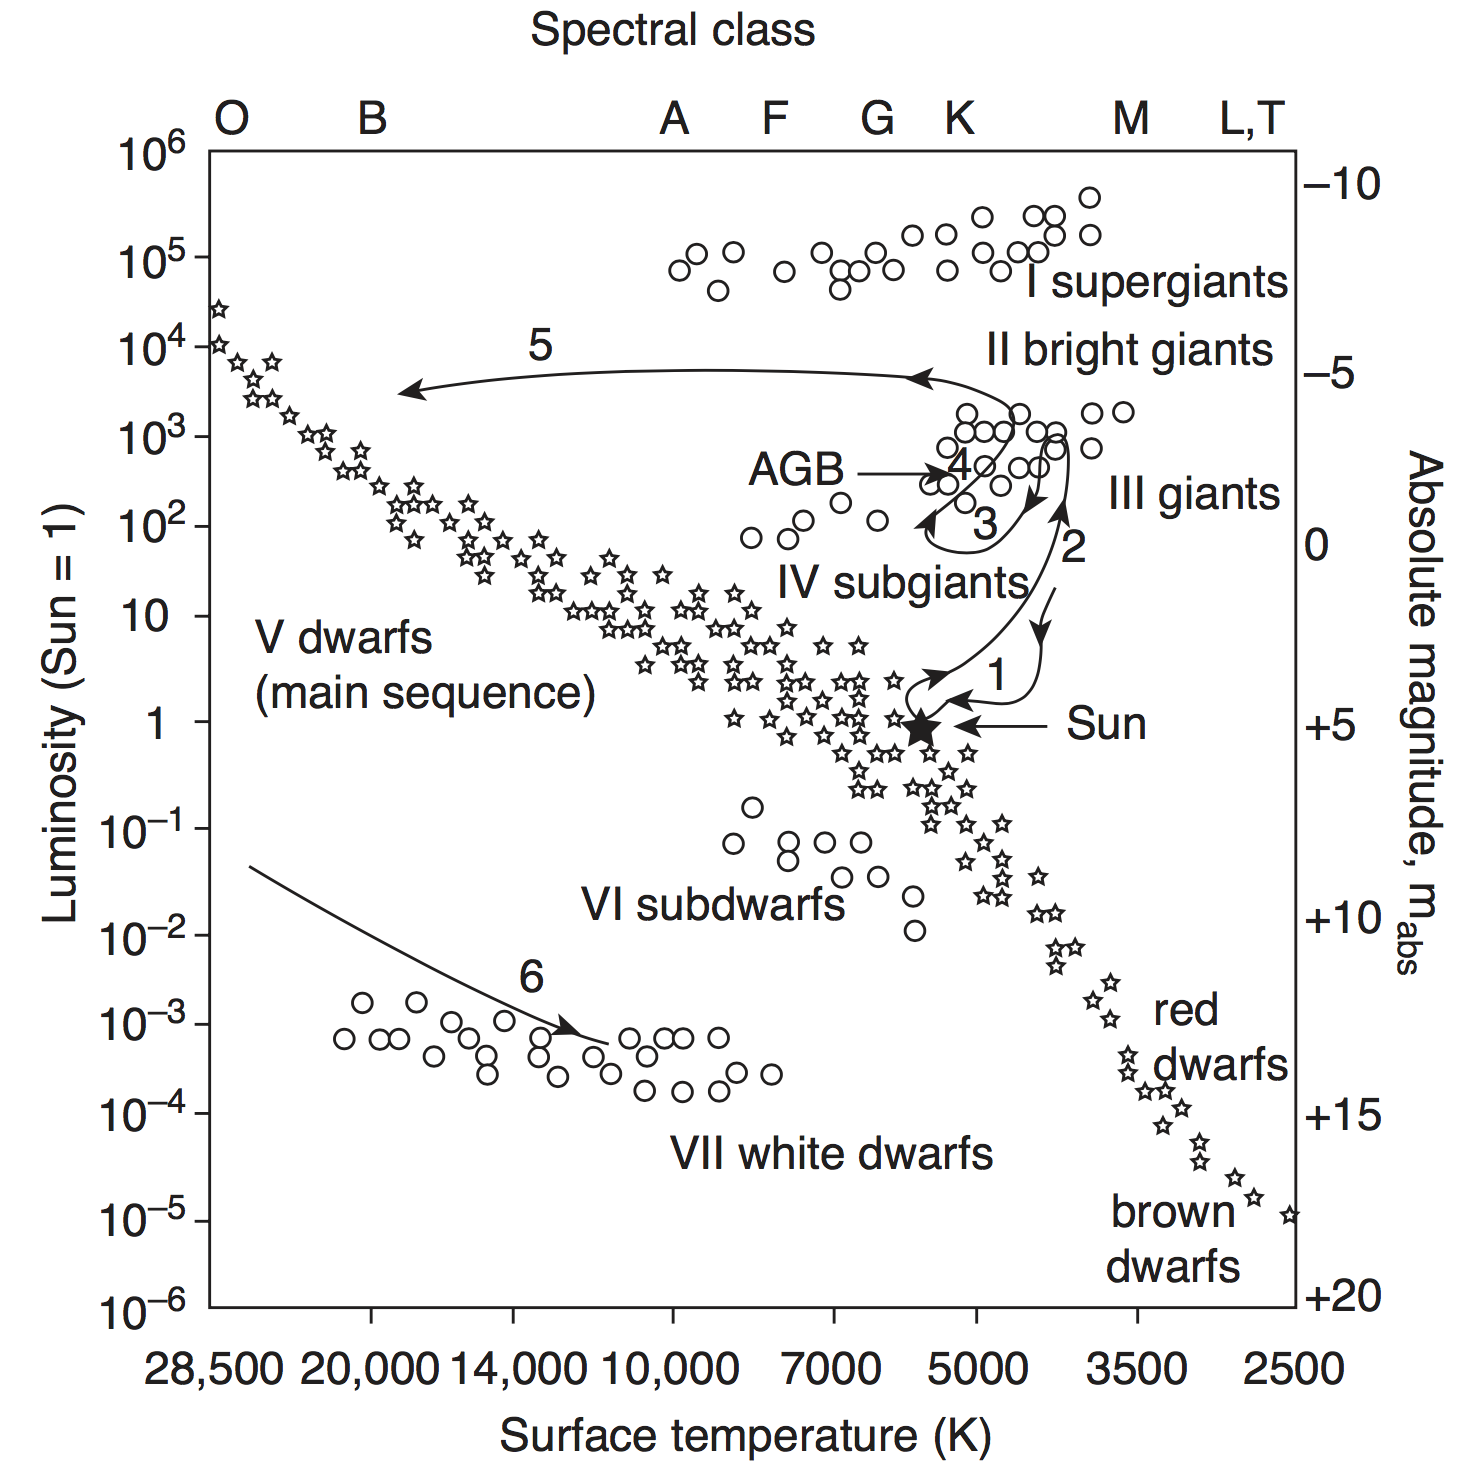
\includegraphics[width=10cm]{figures/HRD.png}}
\end{figure}

\subsubsection{Additional context}

{\noindent}\textbf{Evolution of a $\mathbf{9\,{\rm M_\odot}}$ star:} Figure \ref{fig:hrd9} shows the calculated evolutionary path on the HRD of a $9\,{\rm M_\odot}$ star of solar composition. Letters mark critical points in the course of evolution. Specifically, the various points mark the following events:

\begin{itemize}
    \item A: Beginning of steady hydrogen burning, ZAMS.
    \item C-C0: Exhaustion of hydrogen in the core, and ignition of hydrogen burning in a shell surrounding the hydrogen-exhausted core.
    \item E: Arrival on the Hayashi line, that is, the envelope is (almost) fully convective.
    \item F: Ignition of helium burning in the center.
    \item J: Exhaustion of helium in the core.
    \item JK: Ignition of helium burning in a shell surrounding the helium-exhausted core.
    \item L: Back to the Hayashi line (fully convective envelope).
    \item LM: Early asymptotic giant branch phase (E-AGB).
\end{itemize}

\begin{figure}[h]
    \floatbox[{\capbeside\thisfloatsetup{capbesideposition={right,top},capbesidewidth=4cm}}]{figure}[\FBwidth]
    {\caption{\footnotesize{The evolutionary track in the HRD diagram of a $9\,{\rm M_\odot}$ star with solar composition from the ZAMS all the way to the AGB phase (hydrogen and helium burning in two separate shells). What happens at the labeled points. Source: Renzini et al. (1992, Astrophys. J., 400, 280). Figure taken from Greggio \& Renzini (2011).}}
    \label{fig:hrd9}}
    {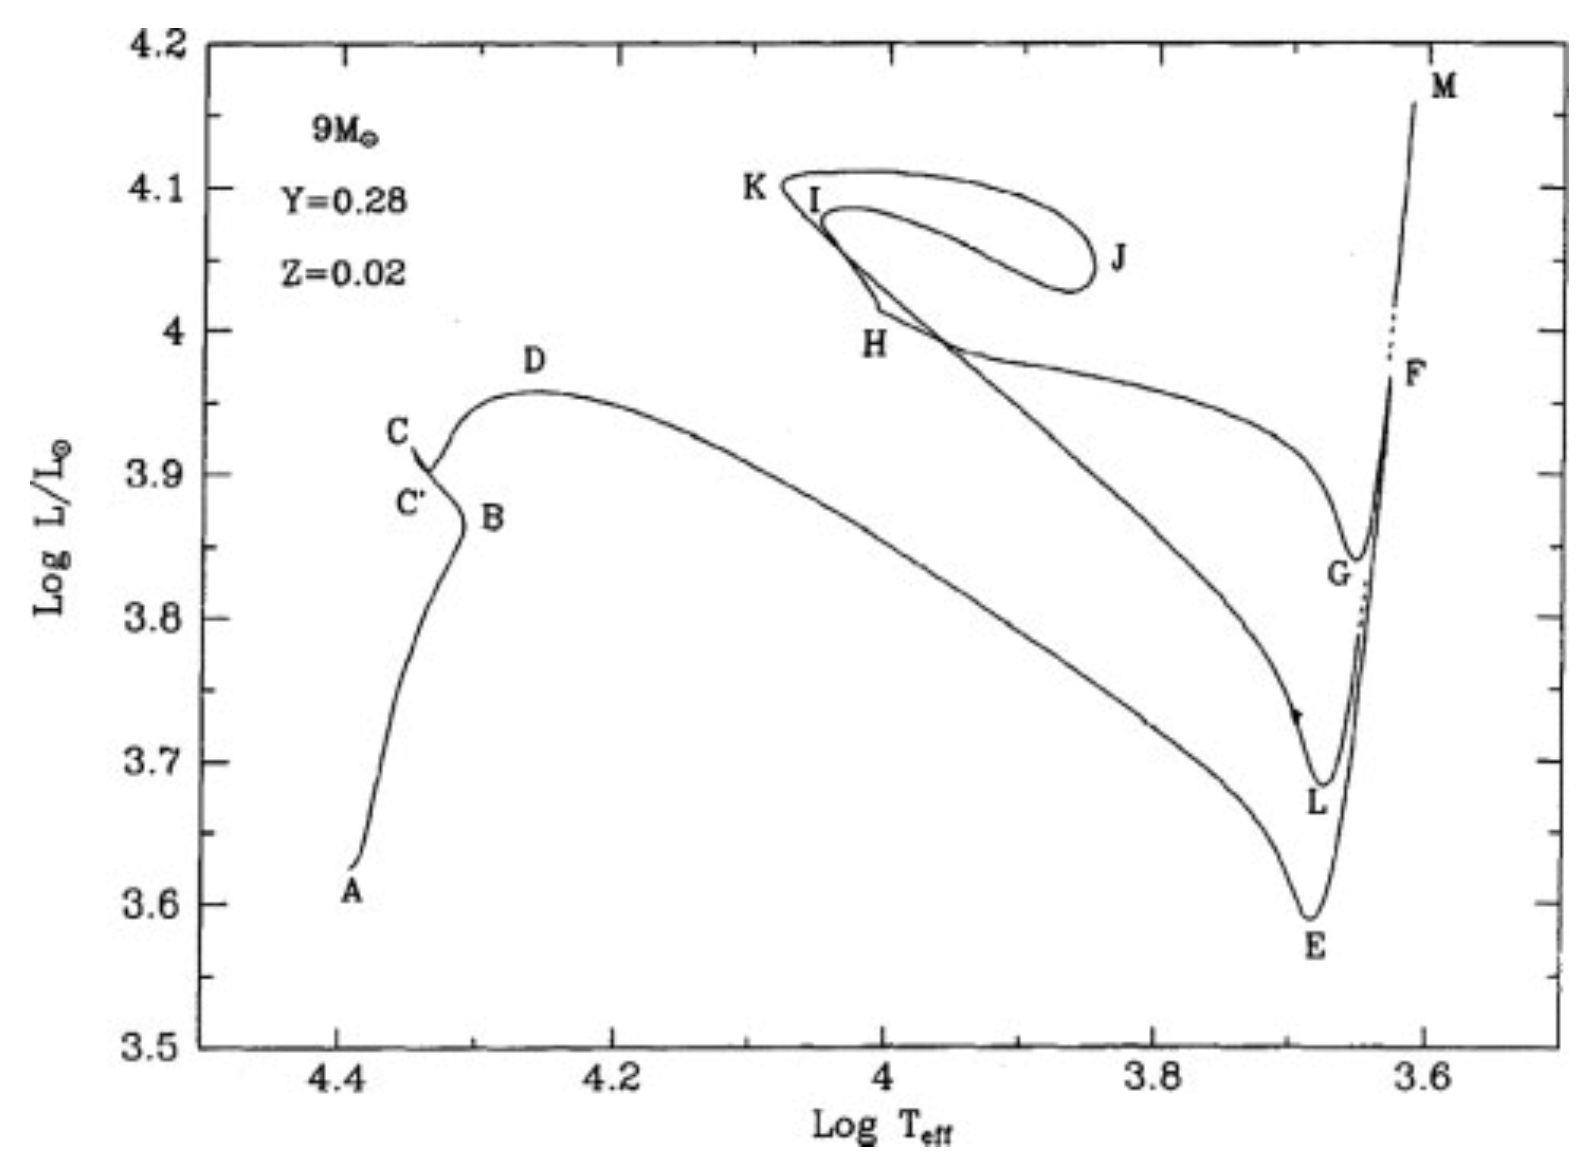
\includegraphics[width=10cm]{figures/HRD_9M.png}}
\end{figure}

{\noindent}Before disclosing what happens at points BDGHI and K (not mentioned in the previous list) it is necessary to introduce a few concepts in the language of stellar model makers. The \textbf{core} is the innermost part of the star, where nuclear reactions have greatly altered the original composition. By \textbf{envelope} one means the outer part of the star, over (most of) which nuclear burning is negligible and whose composition may still be close to the original one.

{\noindent}Next is the concept of \textbf{thermal equilibrium}. \textit{A star is said to be in thermal equilibrium (TE) when the total rate of nuclear energy generation ($L_N$) is almost perfectly equal to its surface luminosity ($L_S$).} TE means that the envelope is able to transfer outside and radiate into space quite precisely the same amount of energy which per unit time is produced by nuclear reactions in the core. If $L_S\simeq L_N$ the star is in TE and its evolution proceeds on a nuclear timescale. Conversely, if $L_S\neq L_N$ the star is out of TE, and its evolution proceeds on a thermal timescale, which usually is much shorter than the nuclear timescale. TE is often broken when the core runs out of fuel or when a new fuel is ignited. A dramatic example of breaking TE is the helium ignition in a degenerate core, called a \textbf{helium flash}. At flash peak $L_N\simeq 10^{10}\,{\rm L_\odot}$ while $L_S\simeq2000\,{\rm L_\odot}$ (and decreases!). The energy that does not escape the star is used to expand the helium core, hence relieving its degeneracy.

\begin{figure}[h]
    \floatbox[{\capbeside\thisfloatsetup{capbesideposition={right,top},capbesidewidth=4cm}}]{figure}[\FBwidth]
    {\caption{\footnotesize{The luminosity radiated from the star's surface as a function of the luminosity released by the stellar core and entering the envelope from its base, for the same track shown in Figure \ref{fig:hrd9}. Labels of relevant points along the sequence are the same as in Figure \ref{fig:hrd9}. Source: Renzini et al. (1992, Astrophys. J., 400, 280). Figure taken from Greggio \& Renzini (2011).}}
    \label{fig:lslb9}}
    {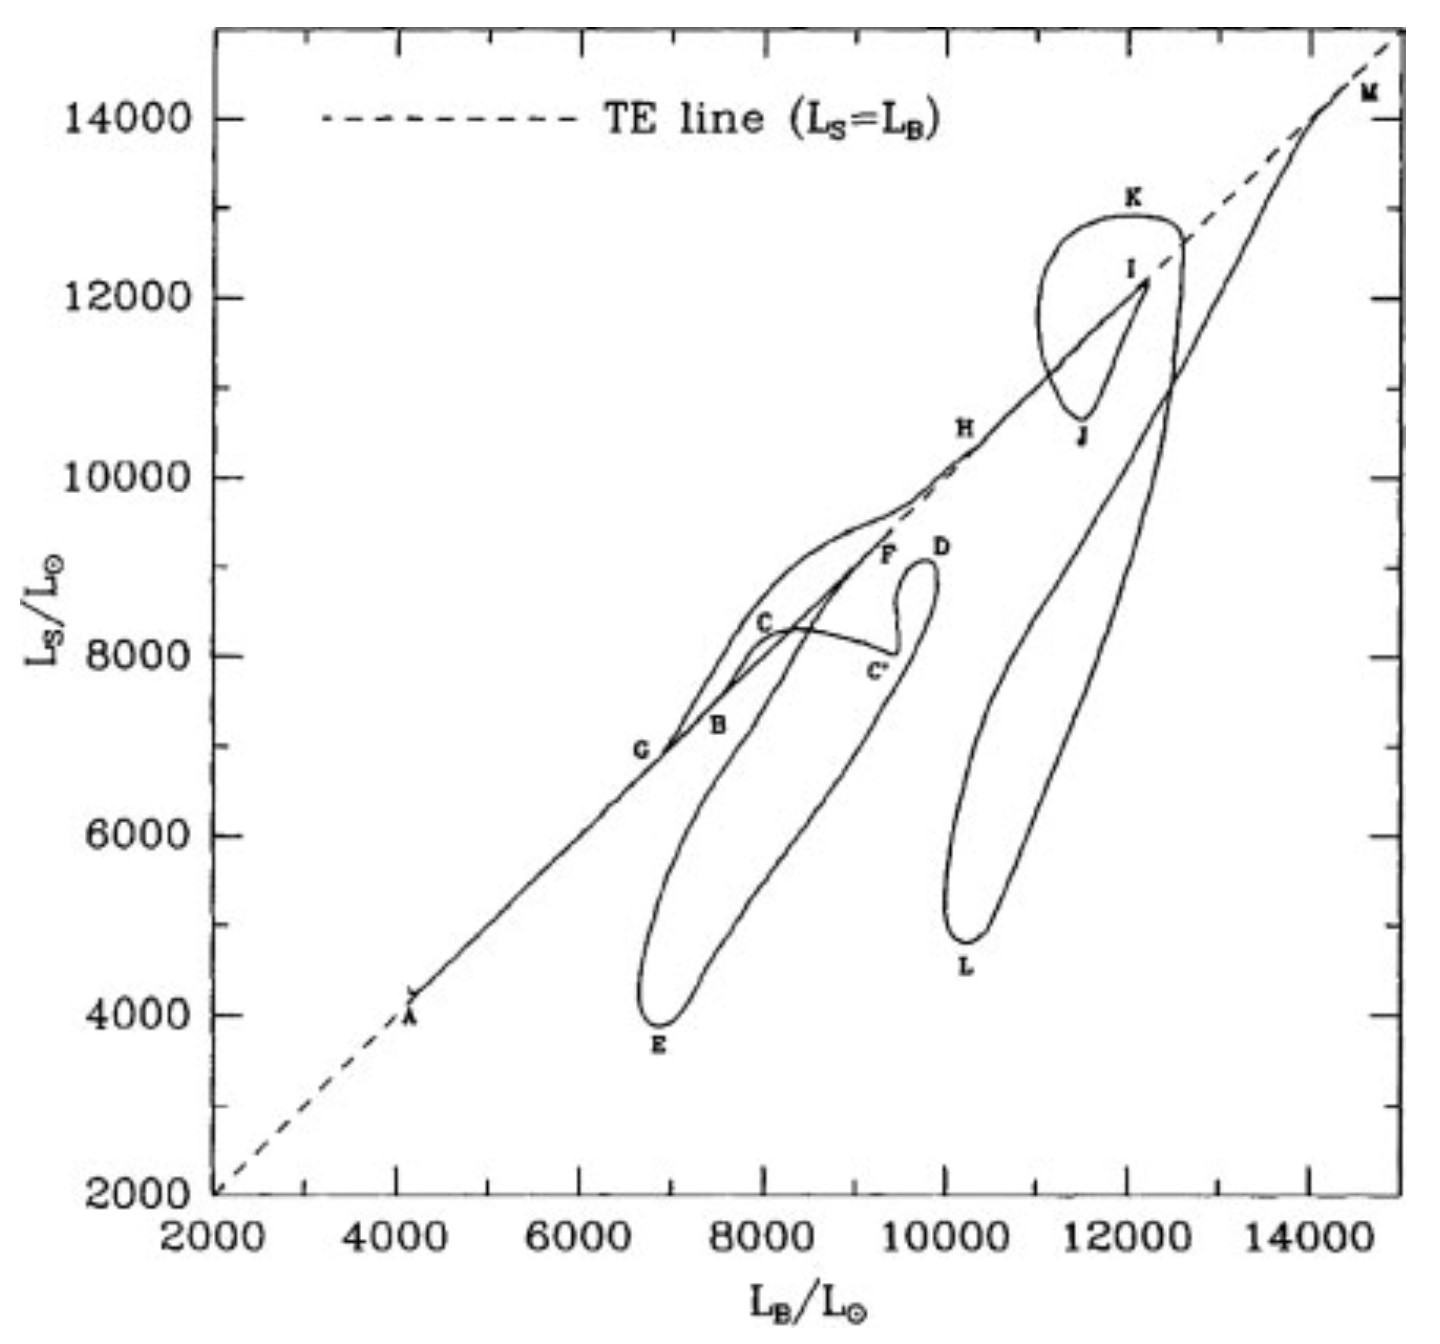
\includegraphics[width=8cm]{figures/LSLB_9M.png}}
\end{figure}

{\noindent}Evolutionary phases in TE and those out of TE can be easily identified by plotting $L_S$ versus $L_N$, or, equivalently, versus the luminosity impinging at the base of the envelope ($L_B$), as shown in Figure \ref{fig:lslb9} relative to the evolution of the same $9\,{\rm M_\odot}$ star model whose HRD is shown in Figure \ref{fig:hrd9}. Letter labels in this figure mark the same events as in Figure \ref{fig:hrd9}, so that one can identify those phases that are in TE and those which are out of it.

{\noindent}Thus, phase AB (which is most of the main sequence phase) proceeds in strict TE, but as hydrogen approaches exhaustion in the core, nuclear burning starts to fall short of keeping in pace with the rate at which energy is being radiated away, the star starts departing from TE and begins to contract (point B). At point B, as the core is running out of fuel the envelope starts losing more energy than it receives, and contracts until at point C hydrogen is effectively exhausted over the central regions, and nuclear energy generation quickly shifts to a shell surrounding a hydrogen-exhausted helium core. The quick readjustment from core to shell burning leaves the star at point C', somewhat out of TE, but then the structure tends to approach again TE, until at point D this tendency is reverted and a major excursion away from TE begins. In stars a little less massive than the one considered here, TE is actually well restored shortly after point C', and yet (as here at point D) TE is broken and stars undergo an extensive loop in the $L_S-L_B$ diagram, as shown in Figure \ref{fig:lslb9}. The journey across the HRD from point D to point E takes place on a thermal timescale, and the star expands to red giant dimensions. Clearly, a thermal instability erupts at point D. This is indeed a quite severe thermal instability, suffice to say from Figure \ref{fig:lslb9} that at the peak of the instability the core releases $\sim7000\,{\rm L_\odot}$ but the envelope radiates away only $\sim4000\,{\rm L_\odot}$, and $\sim3000\,{\rm L_\odot}$ are absorbed for its expansion.

{\noindent}The physical origin of this thermal instability is actually quite easy to understand. During phase C'D the luminosity provided by the hydrogen burning shell steadily increases as the shell moves out in the mass coordinate thanks to its own burning, and sits on a progressively more massive helium core. In response to the increasing luminosity impinging on its base ($L_B$) the envelope slowly expands. By expanding the envelope cools, and by cooling heavy metal ions begin to recombine. Besides being scattered by free electrons, photons now begin to be absorbed by such heavy ions via bound-bound and bound-free transitions: \textit{radiative opacity increases}. This opacity increase is the key factor that determines the onset of the thermal instability. At any point within the star the luminosity transmitted outwards by the radiation field is:

\begin{align*}
    L_r = 4\pi r^2 \frac{4acT^3}{3\kappa\rho} \frac{{\rm d}T}{{\rm d}r} = 4\pi r^2F_r ~ [{\rm erg\,s^{-1}}],
\end{align*}

{\noindent}where $r$ is the distance from the center, $T$ the temperature, $\rho$ the density, $\kappa$ the opacity, and $F_r$ the radiative energy flux. During phase C'D the envelope slowly expands, hence $r^2$ increases while the flux $F_r$ decreases, but their product still increases and the star is approaching TE. However, as this trend continues the increase in opacity accelerates and eventually the flux drops faster than $r^2$ increases, and their product $L_r$ starts to decrease. The decrease happens first near the stellar surface, and then (very quickly) through the whole envelope. At this point the envelope is transferring outwards and radiating away less energy than it receives from the stellar core, that is, $\Delta L=L_B-L_S>0$. But as the envelope expands more ions recombine, opacity increases further, the flux drops even more, the thermal imbalance $L_B-L_S$ increases and expansion accelerates: the stellar envelope is in a thermal runaway, as it becomes more and more unable to radiate away the energy it receives from the stellar interior.

{\noindent}At point E the surface luminosity starts to rise again, $L_B-L_S$ begins to drop, and TE is rapidly restored. What relieves the instability and saves the star from literally falling apart is convection. As the expanding envelope cools, and opacity increases, eventually the radiative gradient $\nabla_{\rm rad}$\footnote{Temperature gradients are defined as $\nabla T(\rho,T,X_i) = (\partial\log T/\partial\log P)$.} exceeds the adiabatic gradient $\nabla_{\rm ad}$, first near the photosphere, where hydrogen is only partly ionized, and then rapidly through the whole envelope. Thus, convection replaces radiative transfer in carrying out energy through the envelope, and the thermal instability is quenched since it was intimately related to the radiative mode of energy transfer. Most of the energy flux in the envelope being now carried by convective motions, the envelope ceases to absorb energy, and the surface luminosity LS starts to increase again: the star now ascends the Hayashi line, until at point F the helium burning reactions ignite in the core.

{\noindent}Following helium ignition, the helium core initiates a very slow expansion, which will last through a major fraction of the helium burning phase. This is because the helium burning core works like a breeder reactor during this stage, that is, it produces more new fuel than it burns. As \textbf{triple-$\mathbf{α}$} reactions produce fresh $^{12}$C, the $^{12}$C($\alpha,\gamma$)$^{16}$O reactions release an increasing amount of energy, and the inner core is forced to expand slightly. Such a modest expansion of the core is sufficient to cause a decrease of temperature and density in the surrounding hydrogen burning shell and the stellar luminosity correspondingly starts to decrease. The star now evolves along the \textbf{Hayashi line} from F to G, burning helium in the core and hydrogen in the shell, until thermal stability is broken again at point G. As the envelope contracts it heats up gradually, and in particular near its base, heavy ions start losing electrons. Hence opacity decreases along with the radiative gradient. As $\nabla_{\rm rad}$ drops below $\nabla_{\rm ad}$ a radiative region appears at the base of the envelope and grows outwards in mass. As this growth progresses the envelope becomes more and more transparent to radiation, until it starts radiating away more energy than it receives from the core: $L_B-L_S$ turns increasingly negative, the envelope starts deflating, but the more it contracts the more ``transparent'' it becomes, and the more energy it loses into space. The thermal instability bringing the star in its envelope deflation from point G to point H is precisely the reverse analog of the thermal instability that causes the runaway expansion from point D to point E. As envelope inflation can be ascribed to a runway recombination of heavy elements in the envelope, envelope deflation is due to a runway ionization of such heavy elements. A comparison of the three figures (Figures \ref{fig:hrd9}-\ref{fig:rvst}) helps in visualizing the onset of the thermal instability and of its results.

\begin{figure}[h]
    \floatbox[{\capbeside\thisfloatsetup{capbesideposition={right,top},capbesidewidth=4cm}}]{figure}[\FBwidth]
    {\caption{\footnotesize{The stellar radius as a function of time for the same track shown in Figure \ref{fig:hrd9}. Labels of relevant points along the sequence are the same as in Figure \ref{fig:hrd9}. Source: Renzini et al. (1992, Astrophys. J., 400, 280). Figure taken from Greggio \& Renzini (2011).}}
    \label{fig:rvst}}
    {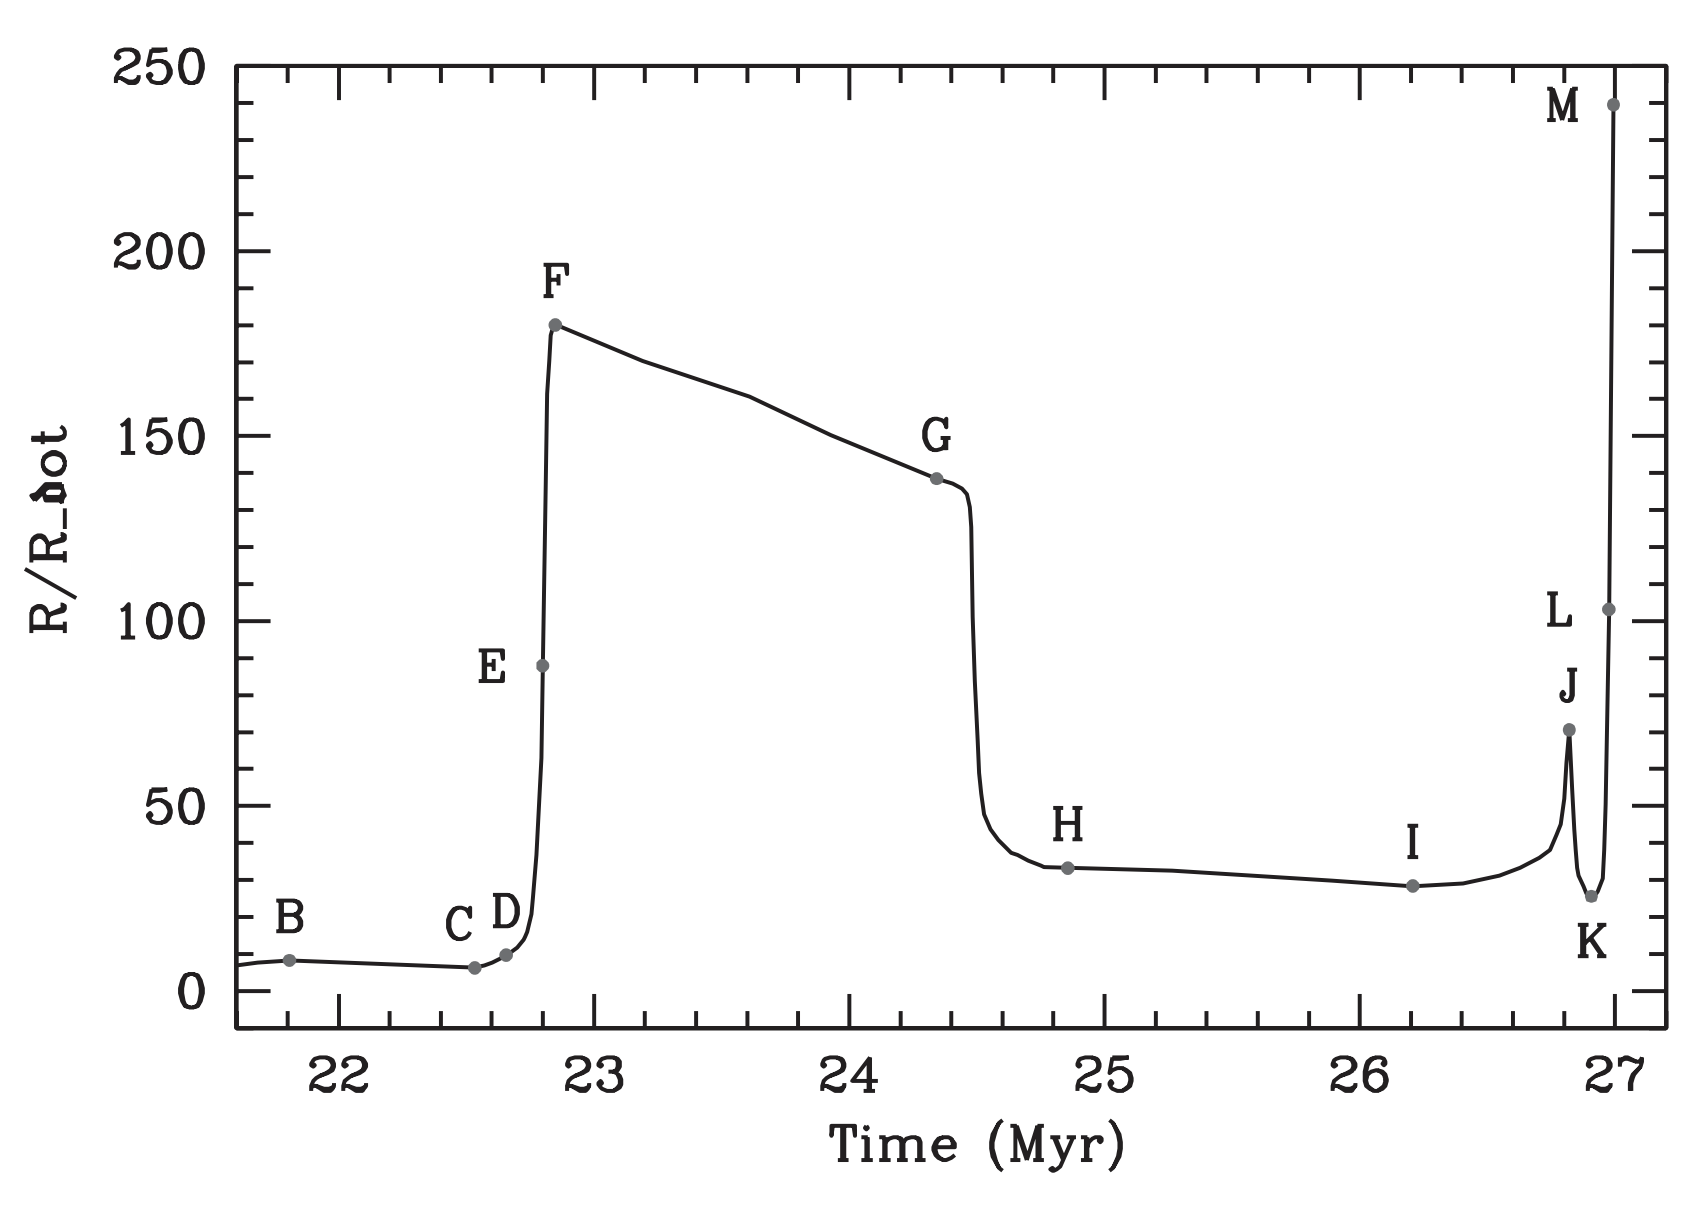
\includegraphics[width=8cm]{figures/RvsT.png}}
\end{figure}

{\noindent}Thus, in this star, the core helium burning phase in thermal equilibrium is spent in two distinct locations in the HRD: part on the Hayashi line as a red giant (F-G) and part as a blue giant (H-I) separated by a runaway contraction out of TE (G-H). This first blue loop (also called the \textbf{Cepheid blue loop}) continues after point I when TE is broken again. Here the envelope is slowly expanding in response to the slowly increasing luminosity from the core and shell burning, when the envelope turns unstable again due to the same physical process already described for the DE phase. 

{\noindent}However, the journey towards the Hayashi line is suddenly interrupted and inverted at point J, which marks the start of the so-called \textbf{second blue loop}. What happens at point J and after is a rather complex series of interconnected events: helium is exhausted in the core, the core contracts and helium burning rapidly shifts from the helium-exhausted CO core to a shell surrounding it; helium shell ignition is quite violent and causes expansion of the helium buffer above this shell: when the expansion front breaks through the hydrogen burning shell temperature and density in the shell drop; burning in the hydrogen shell (which was still providing most of the stellar luminosity) is effectively shut off completely causing a sudden drop of the luminosity impinging on the base of the envelope: $L_B$ drops below $L_S$ and the envelope stops expanding and contracts. In the meantime the strength of the helium burning shell steadily increases until it leads $L_B$ to exceed $L_S$ again, contraction stops and the star resumes at point K its runaway expansion that was temporarily stopped at J. The rest, from K to L to M is quite similar to the DEF phase, with convection replacing radiative transfer in the envelope and TE being rapidly restored, shortly before point M. Figure \ref{fig:rvst} clearly illustrates the dramatic effects of the envelope thermal instabilities on the overall structure of the star. Those phases which are in TE are nearly flat in this plot, that is, the stellar radius changes quite slowly with time. With one exception, those phases which are out of TE are instead nearly vertical, that is, the radius varies very rapidly during such runaway inflations or deflations. The exception is phase BC, which is only modestly out of TE, and contraction is relatively slow.

{\noindent}What happens past point M is still an open issue. A $9\,{\rm M_\odot}$ star lies between two domains: massive stars that eventually undergo core collapse and supernova explosion, and intermediate-mass stars, which shedding all their hydrogen-rich envelope die as a white dwarf. One believes that in a $9\,{\rm M_\odot}$ star carbon is ignited in the central core under only mildly degenerate conditions, and the star keeps ascending along the Hayashi line as a super asymptotic giant branch star experiencing a few thermal pulses in its deeper regions, where hydrogen and helium are still burning in two separate shells. Thus, if the envelope is completely lost in a wind the star leaves an ONeMg white dwarf. If instead mass loss is less severe then the core keeps growing in mass thanks to the active burning shells until electron captures in the core trigger a core collapse and we have a supernova explosion. Clearly the fate critically depends on the strength of the mass loss process.

{\noindent}\textbf{Evolution of a Solar-composition star:} Figure 1.4 shows stellar evolutionary tracks of solar composition, covering a wide range of initial masses, from a $0.8\,{\rm M_\odot}$ star, whose MS evolutionary lifetime is longer than one Hubble time, up to a $20\,{\rm M_\odot}$ model. The evolutionary tracks of stars with mass greater than $20\,{\rm M_\odot}$ are heavily affected by mass loss.

\begin{figure}[h]
    \floatbox[{\capbeside\thisfloatsetup{capbesideposition={right,top},capbesidewidth=4cm}}]{figure}[\FBwidth]
    {\caption{\footnotesize{Evolutionary tracks of solar composition star. The shaded area shows the location of low-mass ($0.55\leq M/M_\odot\leq2$) core helium burning models. Drawn using the YZVAR database (Bertelli, G. et al. 2008, Astron. Astrophys., 484, 815; 2009, Astron. Astrophys., 508, 355). Figure taken from Greggio \& Renzini (2011).}}
    \label{fig:hrdsolar}}
    {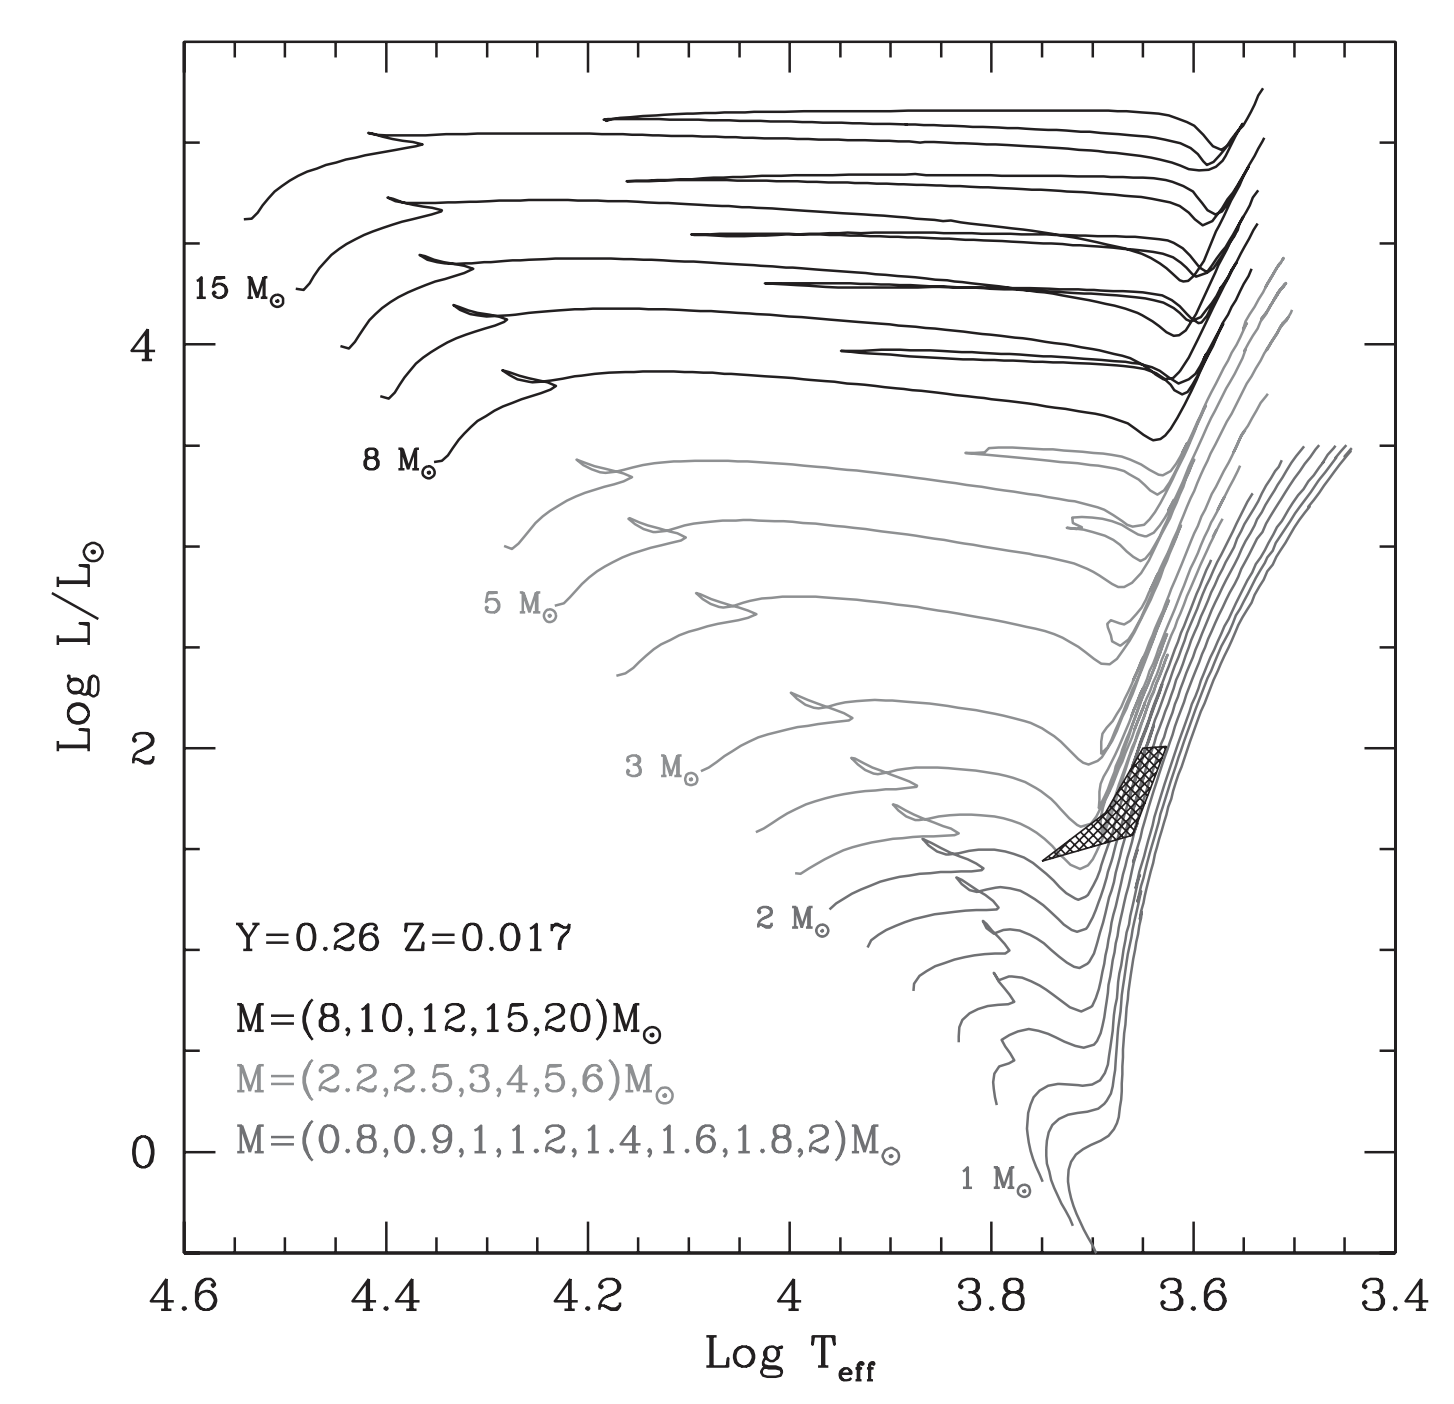
\includegraphics[width=8cm]{figures/HRD_Solar.png}}
\end{figure}

{\noindent}Different gray shades in Figure \ref{fig:hrdsolar} pertain to the different mass ranges as customarily distinguished in stellar evolution: low-mass stars, up to $\lesssim2.2\,{\rm M_\odot}$, intermediate-mass stars, up to $\lesssim8\,{\rm M_\odot}$, and high-mass stars. These ranges correspond to different physical behavior during the evolution of the stars, and the mass limits depend on chemical composition. Low-mass stars develop an \textbf{electron degenerate helium core} after their MS evolution; intermediate mass stars ignite helium under non-degenerate conditions, but develop a \textbf{CO degenerate core} after central helium burning; massive stars experience all successive nuclear burnings up to the production of an \textbf{iron core}.

{\noindent}During their MS evolution, stars with mass below $\sim1\,{\rm M_\odot}$ burn hydrogen through the \textbf{p-p chain}, whose reaction rate is not extremely sensitive to temperature, so that these stars possess a radiative core. As evolution proceeds hydrogen is progressively depleted in the inner core, more in the center than in the periphery, leading to a smooth hydrogen profile from a central minimum up to the initial abundance in the outer layers. On the HRD, the stellar track climbs to higher luminosities and temperatures until the central hydrogen is severely depleted; at this point the effective temperature starts decreasing, producing the turnoff (TO), that is, the maximum temperature point on the MS, which is easily recognizable on the CMD of globular clusters. Shortly after the TO, hydrogen is completely exhausted in the center and the hydrogen shell burning phase starts as a natural progression from the previous core hydrogen burning phase. During shell hydrogen burning, the track forms the subgiant branch (SGB), evolving at (almost) constant luminosity and decreasing temperature until the external convection penetrates deeply inside, and the star becomes almost fully convective at the base of the red giant branch (RGB).

{\noindent}The MS stars (with $M\gtrsim1\,{\rm M_\odot}$) have a convective core, since at least part of the hydrogen burning occurs through the CNO cycle, whose energy generation rate is extremely sensitive to temperature. Because of central mixing, the hydrogen profile is characterized by an inner plateau; as evolution proceeds, the extension of the convective core progressively decreases, leaving behind a gradient of hydrogen abundance. In stars with a convective core, the fuel depletion affects a sizable central region, which starts rapid contraction when approaching fuel exhaustion. This happens at the local minimum effective temperature point during the MS evolution of stars with $M>1\,{\rm M_\odot}$ (Figure \ref{fig:hrdsolar}), which signals the beginning of the overall contraction phase. The evolutionary behavior across this phase and the following runaway expansion has been already described in detail in the previous section.

{\noindent}As already mentioned, the helium core of low-mass stars is (electron) degenerate: this implies that central helium ignition is delayed because core contraction does not lead to an efficient increase of the central temperature. The (almost) fully convective star climbs along the RGB, while the hydrogen burning shell progresses outward, thereby increasing the mass of the helium core. When the core reaches a critical limit, a helium flash occurs off-center, since neutrino losses induce a temperature inversion in the innermost layers. This event in not catastrophic for the star because local expansion removes the degeneracy; instead, a sequence of flashes occurring at progressively inner locations totally remove the core degeneracy. During this phase, which lasts $1\,{\rm Myr}$, the star moves downward along the Hayashi line to settle on the core helium burning locus, either the red clump, or the horizontal branch (HB). The maximum luminosity reached on the RGB (RGB Tip, or TRGB) is a very important feature in the color-magnitude diagram (CMD) of stellar populations because it is virtually independent of mass, and then of evolutionary lifetime. This is because on the one hand the critical mass for helium ignition under degenerate conditions is almost constant ($0.5\,{\rm M_\odot}$), and on the other, along the RGB there exists a core mass-luminosity relation. The evolutionary lifetimes of low-mass stars range from $1\,{\rm Gyr}$ up to the Hubble time, as seen in Figure \ref{fig:hrdsolar}, and all of them experience the helium flash at almost the same luminosity; therefore, the CMD of a stellar population with stars older than $1\,{\rm Gyr}$ will show a prominent TRGB feature whose luminosity is known, thus allowing us to determine the distance of the stellar population. The TRGB luminosity depends slightly on metallicity, being higher for higher metal content. However, by a fortunate combination, the absolute magnitude in the I-band of the TRGB does not depend much on metallicity, for metal-poor populations. This is because the effective temperature at the TRGB also depends on metallicity: the higher $Z$, the cooler the TRGB stars, and the higher the bolometric correction (in absolute value). The trend with metallicity of the bolometric correction to the I-band largely compensates that of the tip luminosity, so that the I-band absolute magnitude of the TRGB ($M_{\rm I,TRGB}$) is almost independent of age and weakly dependent on metallicity of the parent stellar population. This makes $M_{\rm I,TRGB}$ a very effective distance indicator in galaxies.

{\noindent}The luminosity of core helium burning low-mass stars, being fixed by the mass of their hydrogen-exhausted core, is also largely independent of their total mass, thereby providing another distance indicator. However, evolution during the core helium burning phase spreads the red clump stars over $0.6$ magnitudes, as can be seen from the vertical size of the hatched region in Figure \ref{fig:hrdsolar}. In addition, the core mass at helium ignition is not a monotonic function of the total mass, and as the latter increases beyond the limit of the low-mass stars regime ($M_{\rm Hef}$), it decreases, reaches a minimum of about $0.326\,{\rm M_\odot}$, and then increases. As a result, stars with mass just above $M_{\rm Hef}$ start their core helium burning evolution at fainter luminosities, have the longest helium burning lifetimes, and cover a wider range of luminosities, compared to stars with $M<M_{\rm Hef}$. Therefore, the core helium burners of a composite stellar population with a sizable component at ages just below $1\,{\rm Gyr}$ are spread over a wide magnitude range, which limits the use of this feature for distance determinations.

{\noindent}The effective temperature of low mass core helium burning stars depends on the mass of their envelope, a dependence which is very pronounced when the envelope is thinner than for example $0.2\,{\rm M_\odot}$ for $Z\lesssim0.1\,{\rm Z_\odot}$. Below this threshold, the lower the envelope mass, the hotter the core helium burning stars. In a coeval and homogeneous stellar population the core helium burning stars all have virtually the same core mass and then luminosity; a spread of their envelope masses produces a feature on the HRD at about constant (bolometric) magnitude extending over a temperature range. The observational counterpart of this locus is the horizontal branch: a prominent feature in the HRD of globular clusters whose age is old enough to host core helium burning stars with low-mass envelopes. The existence of wide HBs in globular clusters was explained as due to a dispersion of mass lost during the RGB phase, but recently it became apparent that other effects are also at play. Evolutionary tracks during the core helium burning phase exhibit a wide variety of morphologies, depending on their mass, envelope mass, metallicity and helium abundance. At central helium exhaustion, a rapid core contraction leads to shell helium ignition; the model star expands and moves again towards the Hayashi line to start the asymptotic giant branch (AGB) evolutionary stage. However, if the envelope mass is small enough, the shell helium burning phase is entirely spent at high effective temperatures, as an AGB manqu\'e star. The hot HB stars and their AGB manqu\'e progeny are likely responsible for the UV emission from elliptical galaxies which host old stellar populations.

{\noindent}The evolution of intermediate and high-mass stars during the hydrogen and helium burning stages is very similar to what has already been described for the $9\,{\rm M_\odot}$ star. But, following helium exhaustion, intermediate-mass stars behave similarly to low-mass stars. We only notice here that for stars with mass in the vicinity of $M_{\rm Hef}$ the core helium burning phase is spent in a red clump, which becomes a wider and wider blue loop as the model mass grows. Thus, the core helium burning phase of intermediate-mass stars is spent part in the blue and part in the red. The very occurrence of the loop, its extension and the fraction of lifetime spent on each side of the loop, are sensitive to a number of parameters describing the input physics of the models, like metallicity, opacity, convection and others. Therefore, the blue-to-red ratio in stellar populations with stars in this mass range is difficult to interpret. The luminosity of intermediate mass core helium burners is instead a more robust prediction of the models, and can be effectively used as an age indicator of stellar populations.

\begin{table}[t]
    \centering
    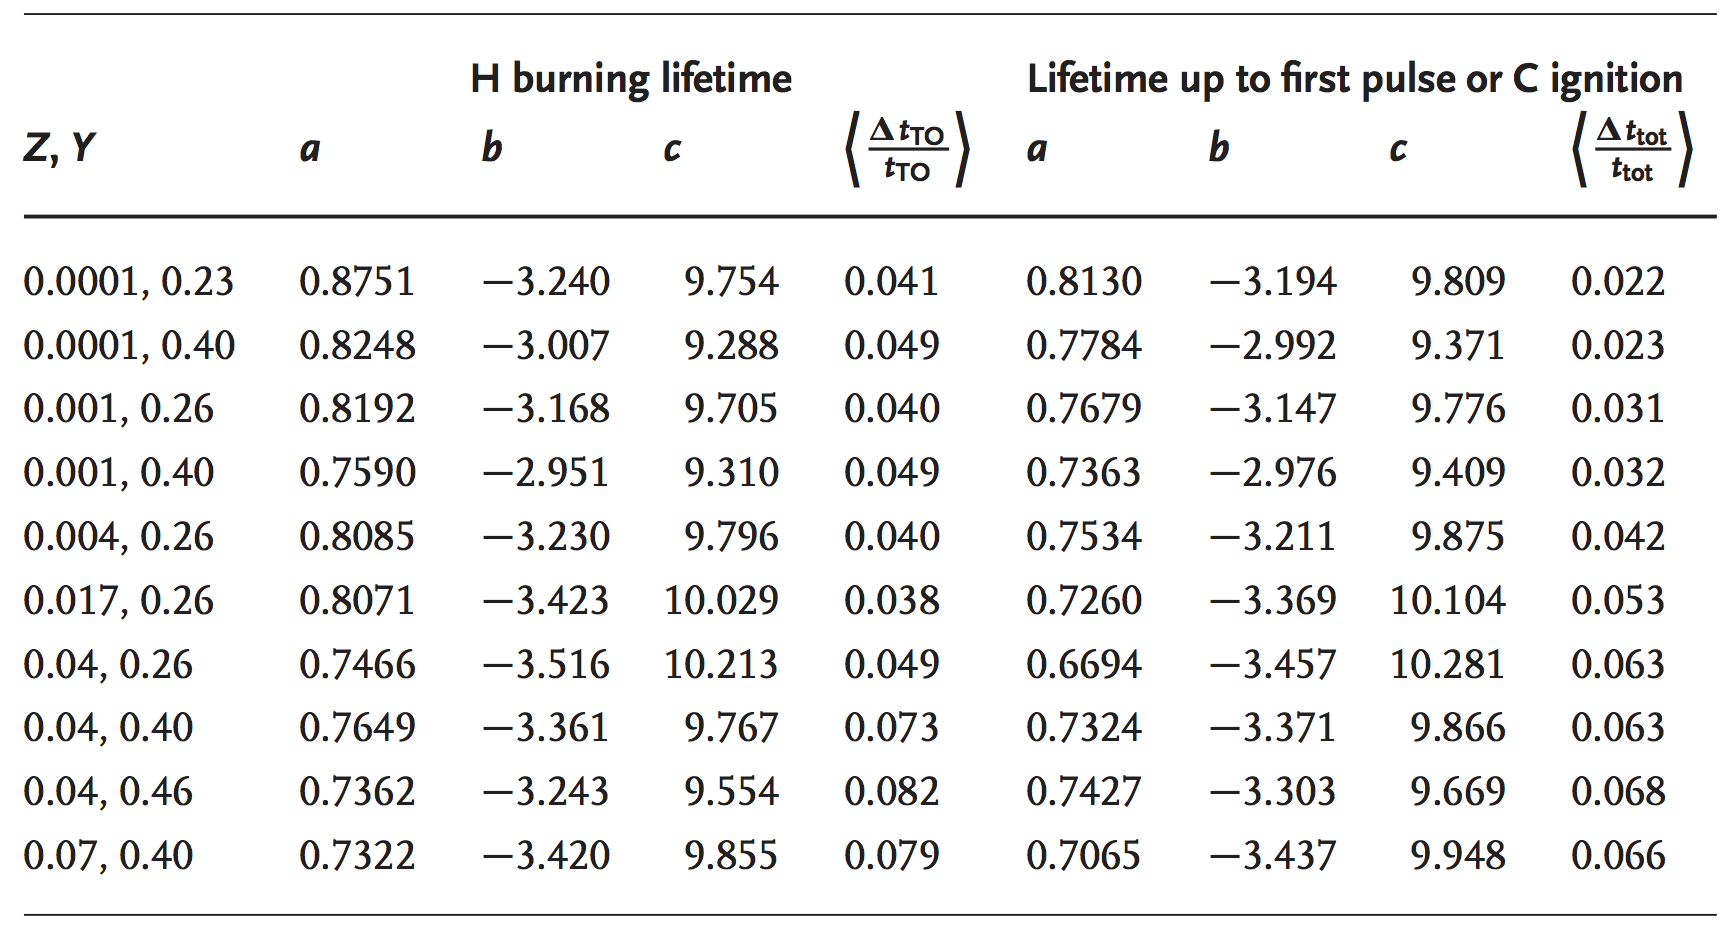
\includegraphics[width=12cm]{figures/HRD_Z_coeff.png}
    \caption{\footnotesize{Coefficients of $\log t$ for various chemical compositions, resulting from the least square fit of the hydrogen burning and the total lifetimes as a function of $M_0$. The fit covers the range $0.6\leq M_0/{\rm M_\odot} \leq20$; columns 5 and 9 report the average relative accuracy on the evolutionary lifetimes at the TO and at the first thermal pulse or central carbon ignition. The YZVAR database (Bertelli, G. et al. 2008, Astron. Astrophys., 484, 815; 2009, Astron. Astrophys., 508, 355) has been used to derive the coefficients. Table taken from Greggio \& Renzini (2011).}}
    \label{table:hrdz_coeff}
\end{table}

{\noindent}\textbf{Dependence on chemical composition:} The evolutionary tracks of given mass are very sensitive to the (initial) helium content ($Y$) and metallicity ($Z$), which control the energy generation rates and the opacity. We briefly illustrate some dependencies relevant to the interpretation of the HR diagram and of the spectral energy distribution of stellar populations.

{\noindent}At a given initial mass, evolutionary lifetimes become shorter as $Y$ increases, because stars with higher molecular weight are more compact, hotter, brighter, hence faster in consuming the hydrogen fuel, of which less is available. Instead, lifetimes become longer as $Z$ increases, because the hydrogen burning models get fainter due to the higher opacity, while the hydrogen fuel reservoir remains virtually unchanged. Table 1.2 lists the values of the coefficients of the following relation:

\begin{align*}
    \log t = a\log^2M_0 + b\log M_0 + c ~ [{\rm yr}],
\end{align*}

{\noindent}adopted to describe the evolutionary lifetimes (in years) as a function of initial mass (in ${\rm M_\odot}$). The parabolic fit over the whole considered mass range is a rather drastic approximation; nevertheless these analytic relations can be useful to estimate evolutionary lifetimes and their dependence on composition.

{\noindent}As mentioned previously, the values of mass defining the low, intermediate and high-mass range depend somewhat on chemical composition. For example $M_{\rm Hef}$ decreases with $Y$ increasing and with $Z$ decreasing. Therefore, an extended RGB on the HRD of a stellar population traces the presence of evolved stars with mass lower than $2.1\,{\rm M_\odot}$ for solar composition, or with mass lower than $1.5\,{\rm M_\odot}$ if $Z=0.001$, $Y=0.4$. However, evolutionary lifetimes at given mass also depend on composition, and, by and large, an extended and well populated RGB is developed in stellar populations older than $1\,{\rm Gyr}$ almost irrespective of chemical composition.

{\noindent}At fixed initial mass, zero age main sequence models are hotter and brighter for a higher helium content, and/or a lower metallicity. Indeed, the locus of the corresponding stars on the HRD (ZAMS) is used to infer the composition of the target stellar population, and is virtually the only way to estimate the helium content of these stars, if $Z$ is known from spectroscopy. The puzzling composition of multiple stellar populations in some galactic globular clusters has been derived from ZAMS fitting.

\begin{figure}[h]
    \floatbox[{\capbeside\thisfloatsetup{capbesideposition={right,top},capbesidewidth=4cm}}]{figure}[\FBwidth]
    {\caption{\footnotesize{a-c) Evolutionary tracks of intermediate-mass stars ($M/{\rm M_\odot}=3,4,5,6,7,8,10$) for different compositions, as labeled. In (a), the open circles mark start and the end of the core helium burning phase. Drawn using the BaSTI database (Pietrinferni, A. et al. 2004, Astrophys. J., 612, 168). the Figure taken from Greggio \& Renzini (2011).}}
    \label{fig:hrdz_int}}
    {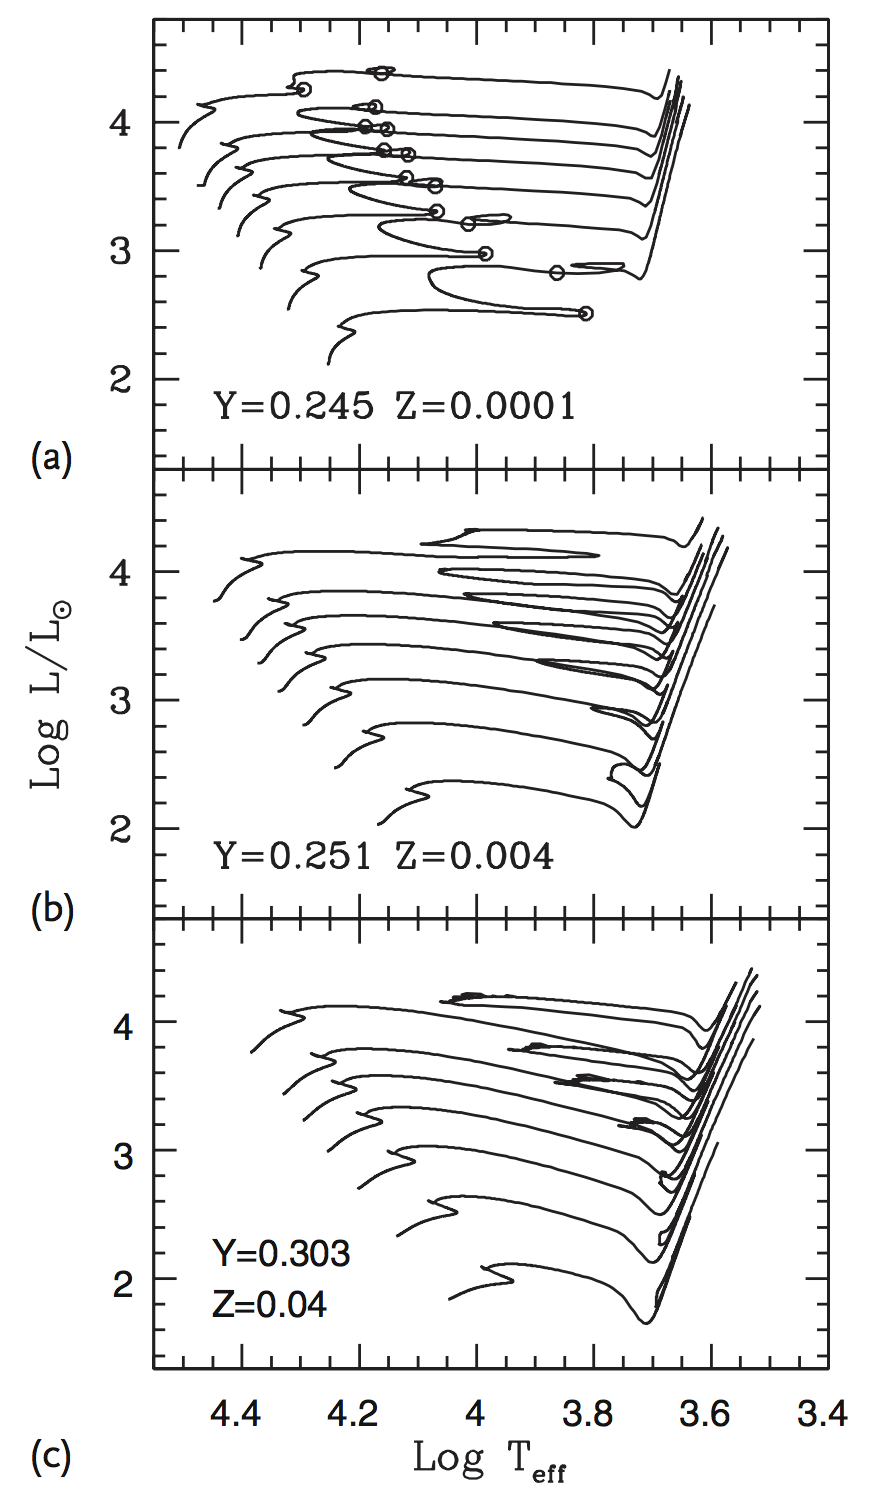
\includegraphics[width=6cm]{figures/HRD_Z_int.png}}
\end{figure}

{\noindent}Figure \ref{fig:hrdz_int} shows some evolutionary tracks of intermediate-mass stars for three different initial compositions. The described trend of the ZAMS with metal content is readily visible, together with some other properties already mentioned: at very low metallicity (Figure \ref{fig:hrdz_int}a) the entire core helium burning phase occurs in the blue part of the HRD, and the thermal runaway in the envelope which brings the model star to the Hayashi track is delayed to the very latest stages. As metallicity increases, the luminosity decrease associated with the thermal runaway gets more and more pronounced: this reflects the progressively higher opacity, and then radiative energy trapping in the envelope. At the same time, at higher metallicity it is more difficult to produce extended blue loops: the $3$ and $4\,{\rm M_\odot}$ tracks at $Z\sim2\,{\rm Z_\odot}$ do not present a blue loop at all, and the loop of the $5\,{\rm M_\odot}$ track is just alluded to. The models in Figure \ref{fig:hrdz_int} are computed adopting classical recipes for the input physics, and even slight modifications of the assumptions lead to dramatic variations of the tracks shape. For example, intermediate-mass models with $Z=0.04$, $Y=0.40$ which adopt a modest overshooting from the convective core lack the loops completely, and the core helium burning phase is totally spent close to the Hayashi line.

{\noindent}Figure \ref{fig:hrdz_low} illustrates the effect of chemical composition on core helium burners of low-mass. The gray tracks in Figure \ref{fig:hrdz_low}a show that at solar composition this evolutionary phase is completely spent in the red, even for masses as low as $0.55\,{\rm M_\odot}$. Conversely, at low metallicity (black lines), low-mass core helium burners are blue, opening the possibility of producing extended HBs in old stellar populations. The tracks in Figure 1.6b show the effect of enhancing the helium abundance: at high metallicity the core helium burning phase is completely spent close to the Hayashi line for a solar helium abundance, but if the helium abundance is high, a blueward excursion occurs during the core helium burning phase which is very wide for low-mass stars. Therefore the production of blue HB stars in old stellar populations can be achieved either assuming heavy mass loss on the RGB, or a high helium content, or both. Actually, the existence of multiple stellar populations with different helium content in NGC 2808 has been first suggested on the basis of its HB stars distribution, and confirmed later from the multiple MSs. Mass loss and helium abundance have indeed an important impact on the HRD of stellar populations, as well as on their spectral energy distribution, since stars in the core helium burning phase provide an important contribution to the total light.

\begin{figure}[t]
    \centering
    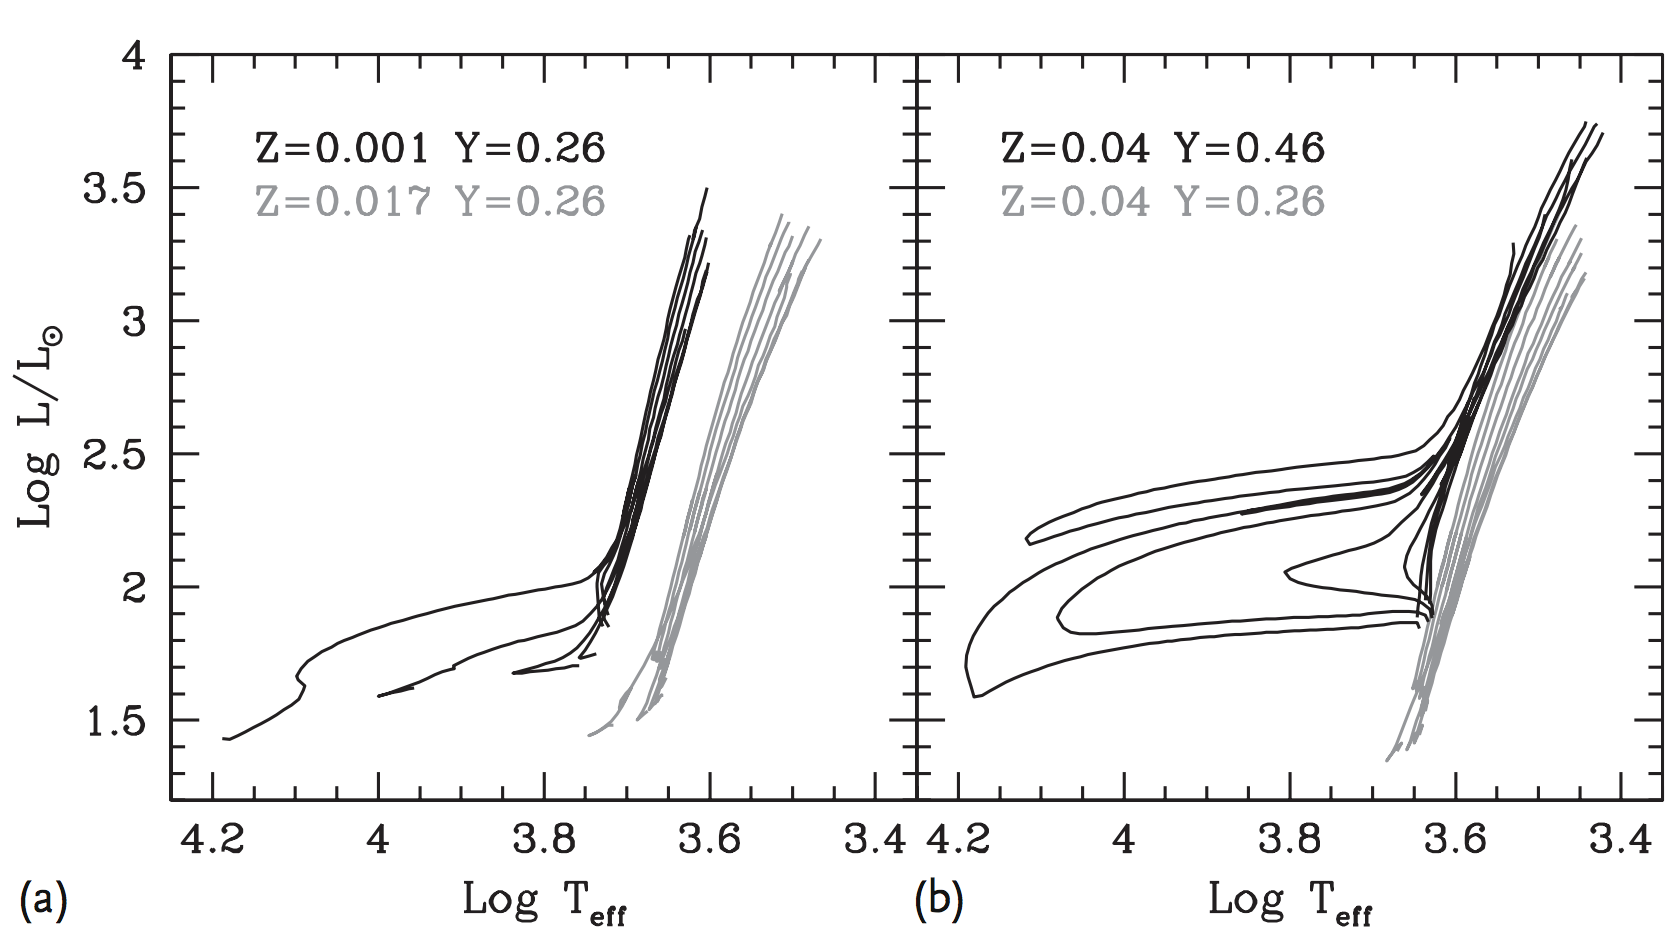
\includegraphics[width=12cm]{figures/HRD_Z_low.png}
    \caption{\footnotesize{(a,b) Evolutionary tracks of low-mass stars during the core helium burning and early AGB phases. The chemical composition is labeled. Initial model masses are $M/{\rm M_\odot}=0.55,0.6,0.65,0.7,1,1.2,1.4,1.6$ except for the ($Z=0.04,Y=0.46$) set, for which the $1.6\,{\rm M_\odot}$ track ignites helium under non-degenerate conditions. Drawn using the YZVAR database (Bertelli, G. et al. 2008, Astron. Astrophys., 484, 815; 2009, Astron. Astrophys., 508, 355). Figure taken from Greggio \& Renzini (2011).}}
    \label{fig:hrdz_low}
\end{figure}

\begin{itemize}
    \item How does metallicity affect this diagram?
    \item Elaborate on the life sequence of low-mass stars.
    \item Elaborate on the life sequence of high-mass stars.
    \item Which direction does radius increase?
    \item What's the functional form for how radius increases as a function of temperature and luminosity?
    \item Why can you use the tip of the red giant branch for distance determination?
    \item How can you use the H-R diagram to determine ages? Which of the two techniques is more accurate?
\end{itemize}

% --------------------------------------------------------------
%               2. 
% --------------------------------------------------------------

\newpage
\subsection{Question 2}

Sketch a plot of radius versus mass for various ``cold'' objects made of normal matter, including planets, brown dwarfs and white dwarfs. Explain the mass-size relationship for rocky and
gaseous objects. Why is there an upper mass limit?

\subsubsection{Short answer}

Using conservation of mass, we can write:

\begin{align*}
    {\rm d}M &= 4\pi r^2\rho{\rm d}r \\
           M &= \frac{4}{3}\pi R^3\rho \\
        \rho &\sim \frac{M}{R^3}.
\end{align*}

{\noindent}Then, using hydrostatic equilibrium, we get:

\begin{align*}
    {\rm d}P &= -\frac{GM}{r^2}\rho{\rm d}r \\
           P &\sim \frac{M}{R}\rho \\
           P &\sim \frac{M^2}{R^4}.
\end{align*}

{\noindent}We know that $P\sim\rho^\alpha$, which we can solve using the equation of state for each object:

{\noindent}\textbf{Planets (rocky)}:
\begin{align*}
    \rho &\sim \frac{M}{R^3} \sim {\rm const} \\
    R &\sim M^{1/3}.
\end{align*}

{\noindent}\textbf{Planets (gas giants)}:
\begin{align*}
    P &\sim \rho^2 \\
    \frac{M^2}{R^4} &\sim \frac{M^2}{R^3} \\
    {\rm indep}&{\rm endent}.
\end{align*}

{\noindent}\textbf{Brown dwarfs/low-mass white dwarfs}:
\begin{align*}
    P &\sim \rho^{5/3} \\
    \frac{M^2}{R^4} &\sim \frac{M^{5/3}}{R^5} \\
    R &\sim M^{-1/3}.
\end{align*}

\begin{figure}[h]
    \centering
    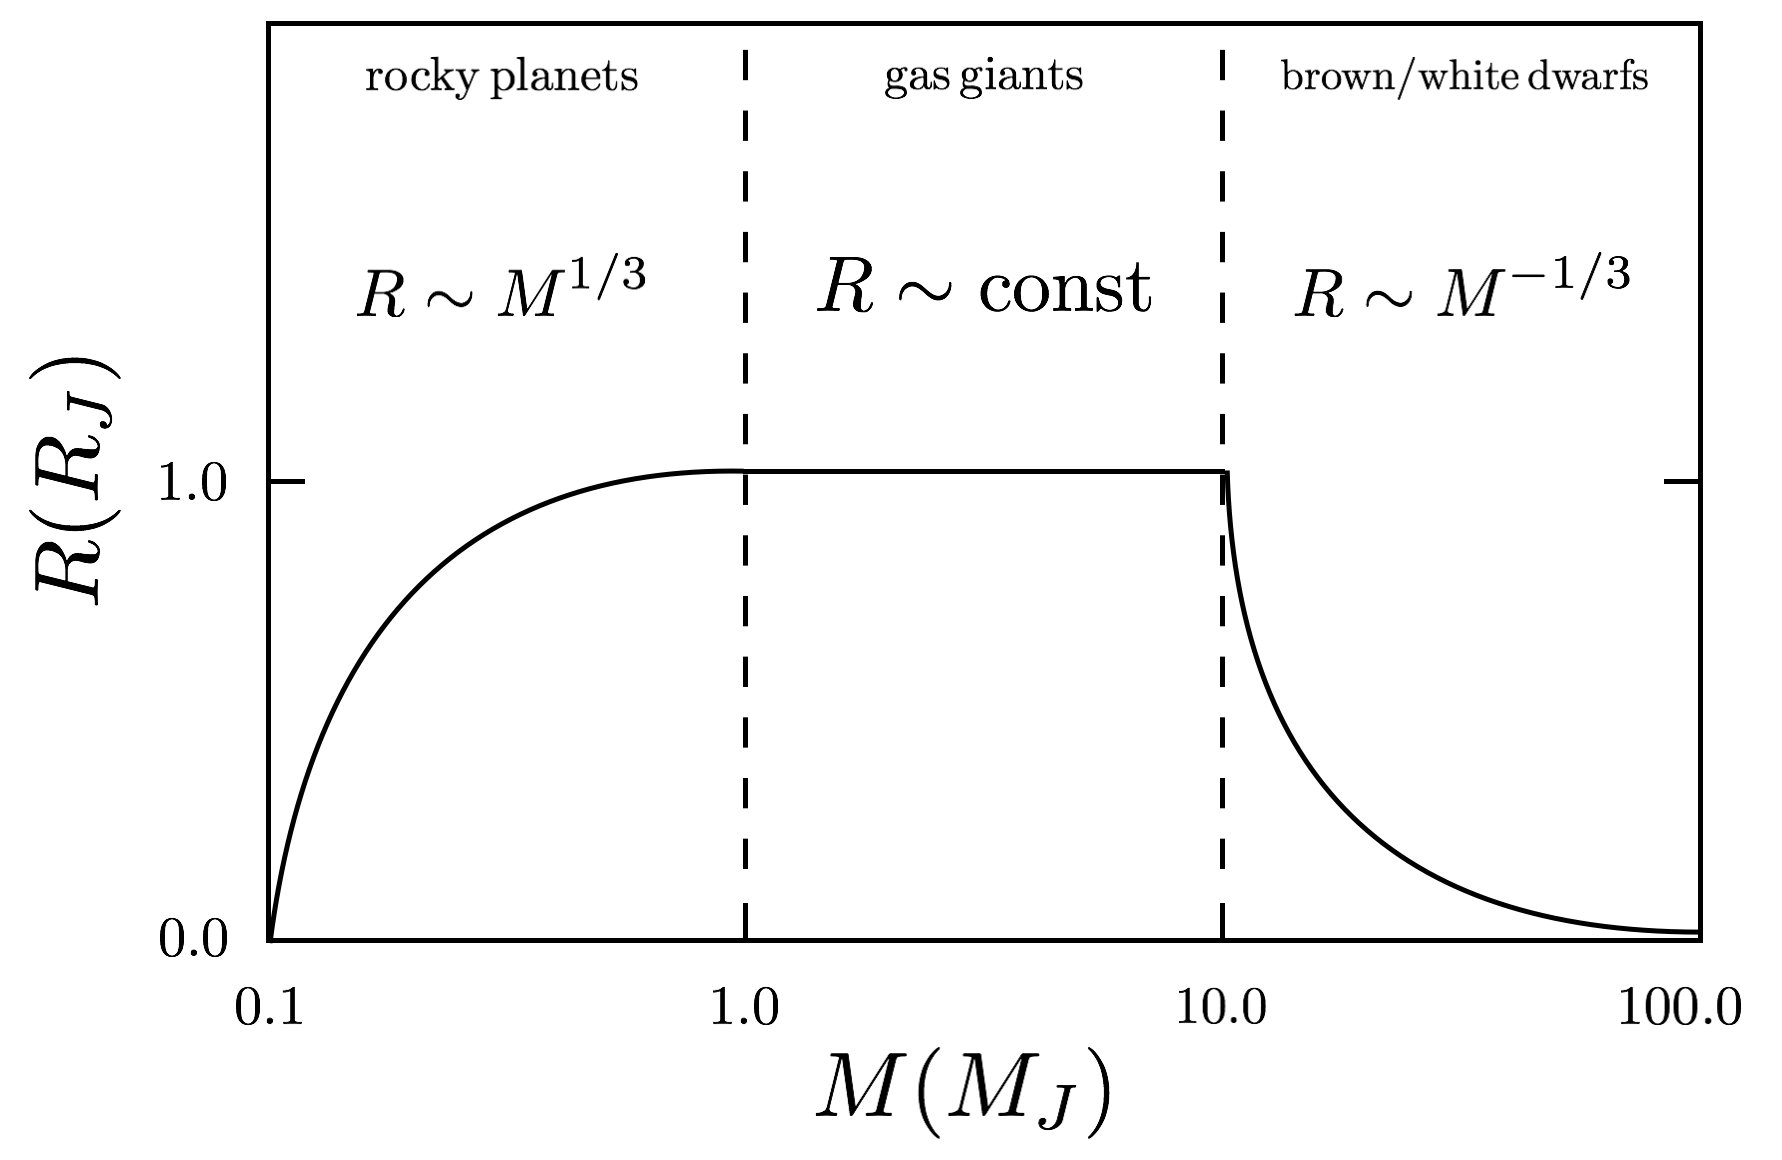
\includegraphics[width=12cm]{figures/RadiusMass.png}
    \caption{\footnotesize{Radius-mass relationship for various cold objects.}}
    \label{fig:radiusmass}
\end{figure}

\newpage
\subsubsection{Follow-up Questions}

\begin{itemize}
    \item How do you calculate the Chandrasekhar mass limit?
    \item Why is Saturn smaller than Jupiter? Or, why do we see a range of radii in extrasolar planets (e.g., hot Jupiters)?
\end{itemize}

% --------------------------------------------------------------
%               3. 
% --------------------------------------------------------------

\newpage
\subsection{Question 3}

Describe the physical conditions that lead to the formation of absorption lines in stars' spectra. What leads to emission lines?

\subsubsection{Short answer}

We can use Kirchoff's laws of radiation to understand the formation of spectral lines in stellar photospheres. These laws are:

\begin{enumerate}
    \item Hot dense gas (e.g., stars) emits blackbody radiation following the description of the Planck function.
    \item Diffuse gas emits emission lines via electronic transitions from a higher state to a lower state, with the energy of the emitted photon corresponding to the energy difference between electronic states.
    \item Cool, diffuse gas in front of a hot dense gas will produce absorption lines on top of the continuum emission. These will occur where the diffuse gas has emission lines, but instead result in the formation of absorption lines instead of emission lines.
\end{enumerate}

{\noindent}So in the example of stellar photospheres, the hot, dense stellar interior produces blackbody emission while the hot, diffuse photosphere produces emission lines. Since there is a temperature gradient in the stellar photosphere, the outer layers of the photosphere will lie at a cooler temperature which allows for the formation of absorption lines.

\subsubsection{Additional context}

If an absorber $X$ is in a level $\ell$ and there is radiation present with photons having an energy equal to $E_u-E_\ell$, where $E_\ell$ and $E_u$ are the energies of levels $\ell$ (for ``lower'') and $u$ (for ``upper''), the absorber can absorb a photon and undergo an upward transition:

\begin{align*}
    \mathbf{absorption:} ~~~ X_\ell+h\nu\rightarrow X_u, ~~~ h\nu=E_u-E_\ell.
\end{align*}

{\noindent}Suppose that we have number density $n_\ell$ of absorbers $X$ in level $\ell$. The rate per volume at which the absorbers absorb photons will obviously be proportional to both the density of photons of the appropriate energy and the number density $n_\ell$, so we can write the rate of change of $n_\ell$ due to photo-absorption by level $\ell$ as

\begin{align*}
    \left(\frac{{\rm d}n_u}{{\rm d}t}\right)_{\ell\rightarrow u} = -\left(\frac{{\rm d}n_\ell}{{\rm d}t}\right)_{\ell\rightarrow u} = n_\ell B_{\ell u}u_\nu, ~~~ \nu=\frac{E_u-E_\ell}{h},
\end{align*}

{\noindent}where $u_\nu$ is the \textbf{radiation energy density per unit frequency}, and the proportionality constant $B_{\ell u}$ is the \textbf{Einstein B coefficient} for the transition $\ell\rightarrow u$.

{\noindent}An absorber $X$ in an excited level $u$ can decay to a lower level $\ell$ with emission of a photon. There are two ways this can happen:

\begin{align*}
    \mathbf{spontaneous~emission:} X_u&\rightarrow X_\ell+h\nu, ~~~ \nu=(E_u-E_\ell)/h, \\
    \mathbf{stimulated~emission:} X_u+h\nu&\rightarrow X_\ell+2h\nu, ~~~ \nu=(E_u-E_\ell)/h.
\end{align*}

{\noindent}\textbf{Spontaneous emission} is a random process, independent of the presence of a radiation field, with a probability per unit time $A_{u\ell}$ -- the \textbf{Einstein A coefficient}.

{\noindent}\textbf{Stimulated emission} occurs if photons of the identical frequency, polarization, and direction of propagation are already present, and the rate of stimulated emission is proportional to the density of these photons. Thus the total rate of depopulation of level $u$ due to emission of photons can be written

\begin{align*}
    \left(\frac{{\rm d}n_\ell}{{\rm d}t}\right)_{u\rightarrow\ell} = -\left(\frac{{\rm d}n_u}{{\rm d}t}\right)_{u\rightarrow\ell} = n_u(A_{u\ell}+B_{u\ell}u_\nu), ~~~ \nu=\frac{E_u-E_\ell}{h},
\end{align*}

{\noindent}where the coefficient $B_{u\ell}$ is the \textbf{Einstein B coefficient} for the downward transition $u\rightarrow\ell$. Thus we now have three coefficients characterizing radiative transitions between levels $u$ and $\ell$: $A_{u\ell}$, $B_{u\ell}$ and $B_{\ell u}$. We will now see that they are not independent of one another.

{\noindent}In TE, the radiation field becomes the ``blackbody'' radiation field, with intensity given by the \textbf{blackbody spectrum}

\begin{align*}
    B_\nu(T) = \frac{2h\nu^2}{c^2} \frac{1}{\exp(h\nu/k_BT) - 1} ~ [{\rm erg\,s^{-1}\,cm^{-2}\,Hz^{-1}\,sr^{-1}}],
\end{align*}

{\noindent}with specific energy density

\begin{align*}
    (u_\nu)_{\rm LTE} = \frac{4\pi}{c}B_\nu(T) = \frac{8\pi h\nu^3}{c^3}\frac{1}{e^{h\nu/k_BT}-1} ~ [{\rm erg\,s^{-2}\,cm^{-1}\,Hz^{-1}\,sr^{-1}}].
\end{align*}

{\noindent}If we place absorbers $X$ into a blackbody radiation field, then the net rate of change of level $u$ is

\begin{align*}
    \frac{{\rm d}n_u}{{\rm d}t} &= \left(\frac{{\rm d}n_u}{{\rm d}t}\right)_{\ell\rightarrow u} + \left(\frac{{\rm d}n_u}{{\rm d}t}\right)_{u\rightarrow\ell} \\
    &= n_\ell B_{\ell u}\frac{8\pi h\nu^3}{c^3} \frac{1}{\exp(h\nu/k_BT) - 1} - n_u \left(A_{u\ell}+B_{u\ell}\frac{8\pi h\nu^3}{c^3} \frac{1}{\exp(h\nu/k_BT) - 1}\right).
\end{align*}

{\noindent}If the absorbers are allowed to come to equilibrium with the radiation field, levels $\ell$ and $u$ must be populated according to $n_u/n_\ell = (g_u/g_\ell)e^{(E_\ell−E_u)/k_BT}$, with ${\rm d}n_u/{\rm d}t = 0$. From the equation above, it is easy to show that $B_{u\ell}$ and $B_{\ell u}$ must be related to $A_{u\ell}$ by

\begin{align*}
    B_{u\ell} &= \frac{c^3}{8\pi h\nu^3}A_{u\ell} ~ [{\rm s^{-1}}], \\
    B_{\ell u} &= \frac{g_u}{g_\ell}B_{u\ell} = \frac{g_u}{g_\ell}\frac{c^3}{8\pi h\nu^3} A_{u\ell} ~ [{\rm s^{-1}}].
\end{align*}

{\noindent}Thus the strength of stimulated emission ($B_{u\ell}$) and absorption ($B_{\ell u}$) are both determined by $A_{u\ell}$ and the ratio $g_u/g_\ell$.

{\noindent}Rather than discussing absorption and stimulated emission in terms of the radiation energy density $u_\nu$, it is helpful to characterize the intensity of the radiation field by a dimensionless quantity, the photon occupation number $n_\gamma$:

\begin{align*}
    n_\gamma &\equiv \frac{c^2}{2h\nu^3} I_\nu ~ [{\rm dimensionless}], \\
    \bar{n}_\gamma &\equiv \frac{c^2}{2h\nu^3} \bar{I}_\nu = \frac{c^3}{8\pi h\nu^3} u_\nu ~ [{\rm dimensionless}],
\end{align*}

{\noindent}where the bar denotes averaging over directions. With this definition of $n_\gamma$, we can rewrite equations for $({\rm d}n_u/{\rm d}t)_{\ell\rightarrow u}$ and $({\rm d}n_\ell/{\rm d}t)_{u\rightarrow\ell}$ as simply

\begin{align*}
    \left(\frac{{\rm d}n_\ell}{{\rm d}t}\right)_{u\rightarrow\ell} &= n_uA_{u\ell}(1+\bar{n}_\gamma),\\
    \left(\frac{{\rm d}n_u}{{\rm d}t}\right)_{\ell\rightarrow u} &= n_\ell \frac{g_u}{g_\ell}A_{u\ell}\bar{n}_\gamma.
\end{align*}

{\noindent}If the radiation field depends on frequency in the vicinity of the transition frequency $\nu_{u\ell}$, then $n_\gamma$ needs to be averaged over the emission and absorption profiles in the above two equations.

{\noindent}From the first of the above two equations, we immediately see that the photon occupation number $n_\gamma$ determines the relative importance of stimulated and spontaneous emission: stimulated emission is unimportant when $\bar{n}_\gamma\ll1$, but should otherwise be included in analyses of level excitation.

{\noindent}\textbf{Absorption cross section:} Having determined the rate at which photons are absorbed by an absorber exposed to electromagnetic radiation, it is useful to recast this in terms of an absorption cross section. The photon density per unit frequency is just $u_\nu/h\nu$. Let $\sigma_{\ell u}(\nu)$ be the cross section for absorption of photons of frequency $\nu$ with resulting $\ell\rightarrow u$ transition. The absorption rate is then

\begin{align*}
    \left(\frac{{\rm d}n_u}{{\rm d}t}\right)_{\ell\rightarrow u}= n_\ell \int \sigma_{\ell u}(\nu)c \frac{u_\nu}{h\nu}{\rm d}\nu \approx n_\ell u_\nu \frac{c}{h\nu} \int \sigma_{\ell u}(\nu){\rm d}\nu ~ [{\rm s^{-1}}],
\end{align*}

{\noindent}where we have assumed that $u_\nu$ (and $h\nu$) do not vary appreciably over the line profile of $\sigma_{u\ell}$. Thus

\begin{align*}
    B_{\ell u} = \frac{c}{h\nu} \int \sigma_{\ell u}(\nu){\rm d}\nu ~ [{\rm s^{-1}}],
\end{align*}

{\noindent}and, using our equation that relates $B_{\ell u}$ to $A_{u\ell}$, we obtain the integral over the absorption cross section:

\begin{align*}
    \int \sigma_{\ell u}(\nu){\rm d}\nu = \frac{g_u}{g_\ell} \frac{c^2}{8\pi\nu_{\ell u}^2}A_{u\ell} ~ [{\rm Hz\,cm^2}].
\end{align*}

{\noindent}Thus we may relate the monochromatic absorption cross section $\sigma_{\ell u}(\nu)$ to a normalized line profile $\phi_\nu$:

\begin{align*}
    \sigma_{\ell u}(\nu) = \frac{g_u}{g_\ell} \frac{c^2}{8\pi\nu_{\ell u}^2}A_{u\ell} \phi_\nu ~ [{\rm cm^2}], ~~~ \int\phi_\nu{\rm d}\nu =1.
\end{align*}

{\noindent}\textbf{Intrinsic line profile:} The intrinsic line profile is characterized by a normalized profile function $\phi_\nu^{\rm intr}$:

\begin{align*}
    \sigma_\nu^{\rm intr} = \frac{\pi e^2}{m_ec^2}f_{\ell u} \phi_\nu^{\rm intr} ~ [{\rm cm^2}], ~~~ \int\phi_\nu^{\rm intr}{\rm d}\nu =1.
\end{align*}

{\noindent}The intrinsic line profile of an absorption line is normally described by the \textbf{Lorentz line profile} function:

\begin{align*}
    \phi_\nu^{\rm intr} = \frac{4\gamma_{u\ell}}{16\pi^2(\nu-\nu_{u\ell})^2+\gamma_{u\ell}^2} ~ [{\rm erg\,s^{-1}\,cm^{-2}\,sr^{-1}}],
\end{align*}

{\noindent}where $\nu_{u\ell} \equiv (E_u-E_\ell)/h$. The Lorentz profile provides an accurate (but not exact)\footnote{The line profile is more accurately given by the \textbf{Kramers-Heisenberg formula}; Lee (2003) discusses application of this formula to the Lyman $\alpha$ line.} approximation to the actual line profile. The Lorentz line profile has a \textbf{full width at half maximum} (FWHM) of

\begin{align*}
    (\Delta\nu)_{\rm FWHM}^{\rm intr} = \frac{\gamma_{u\ell}}{2\pi} ~ [{\rm Hz}].
\end{align*}

{\noindent}The intrinsic width of the absorption line reflects the uncertainty in the energies of levels $u$ and $\ell$ due to the finite lifetimes of these levels\footnote{The \textbf{Heisenberg uncertainty principle} $\Delta E\Delta t\geq\hbar$ implies that an energy level $u$ has a width $\Delta E_u\approx\hbar/\tau_u$, where $\tau_u$ is the level lifetime.} against transitions to all other levels, including both radiative and collisional transitions. If the primary process for depopulating levels $u$ and $\ell$ is spontaneous decay (as is often the case in the ISM), then

\begin{align*}
    \gamma_{u\ell} \equiv \gamma_{\ell u} = \sum_{E_j<E_u}A_{uj} + \sum_{E_j<E_\ell}A_{\ell j}.
\end{align*}

{\noindent}In the case of a \textbf{resonance line}, where $\ell$ is the ground state, the second sum vanishes.

{\noindent}\textbf{Doppler broadening; The voigt line profile:} Atoms and ions are generally in motion, and the velocity distribution is often approximated by a Gaussian, this being of course the correct form if the velocities are entirely due to thermal motions:

\begin{align*}
    p_v = \frac{1}{\sqrt{2\pi}}\frac{1}{\sigma_v} e^{-(v-v_0)^2/2\sigma_v^2} = \frac{1}{\sqrt{\pi}}\frac{1}{b} e^{-(v-v_0)^2/b^2},
\end{align*}

{\noindent}where $p_v{\rm d}v$ is the probability of the velocity along the line of sight being in the interval $[v,v+{\rm d}v]$, $\sigma_v$ is the one-dimensional velocity dispersion, and $b$ is the the \textbf{broadening parameter}, $b\equiv\sqrt{2}\sigma_v$.

{\noindent}The width of the velocity distribution is also sometimes specified in terms of the FWHM; for a Gaussian distribution of velocities, this is just

\begin{align*}
    (\Delta v)_{\rm FWHM} = \sqrt{8\ln2}\sigma_v = 2\sqrt{\ln2}b ~ [{\rm m\,s^{-1}}].
\end{align*}

{\noindent}If the velocity dispersion is entirely due to thermal motion with kinetic temperature $T=10^4T_4\,{\rm K}$, then

\begin{align*}
    \sigma_v &= \left(\frac{k_BT}{M}\right)^{1/2} = 9.12\left(\frac{T_4}{M/{\rm amu}}\right)^{1/2} ~ [{\rm km\,s^{-1}}] \\
    b &= \left(\frac{2k_BT}{M}\right)^{1/2} = 12.90\left(\frac{T_4}{M/{\rm amu}}\right)^{1/2} ~ [{\rm km\,s^{-1}}] \\
    (\Delta v)_{\rm FWHM}^{\rm therm} &= \left[\frac{(8\ln2)k_BT}{M}\right]^{1/2} = 21.47\left(\frac{T_4}{M/{\rm amu}}\right)^{1/2} ~ [{\rm km\,s^{-1}}].
\end{align*}

{\noindent}The intrinsic absorption line profile $\phi_\nu^{\rm intr}$ must be convolved with the velocity distribution of the absorbers to obtain the line profile

\begin{align*}
    \phi_\nu = \int p_v(v) \frac{4\gamma_{u\ell}}{16\pi^2[\nu-(1-v/c)\nu_{u\ell}]^2 + \gamma_{u\ell}^2}{\rm d}v ~ [{\rm erg\,s^{-1}\,cm^{-2}\,sr^{-1}}],
\end{align*}

{\noindent}where $p_v{\rm d}v$ is the probability of the absorber having radial velocity in the interval $[v,v+{\rm d}v]$. If the absorbers have a \textbf{Maxwellian} (i.e., Gaussian) one-dimensional velocity distribution $p_v$, then the absorption line will have a so-called \textbf{Voigt line profile}:

\begin{align*}
    \phi_\nu^{\rm Voigt} \equiv \frac{1}{\sqrt{2\pi}} \int \frac{e^{-v^2/2\sigma_v^2}}{\sigma_v} p_v(v) \frac{4\gamma_{u\ell}}{16\pi^2[\nu-(1-v/c)\nu_{u\ell}]^2 + \gamma_{u\ell}^2}{\rm d}v ~ [{\rm erg\,s^{-1}\,cm^{-2}\,sr^{-1}}].
\end{align*}

{\noindent}Unfortunately, the Voigt line profile cannot be obtained analytically except for limiting cases.5 However, if, as is generally the case, the one-dimensional velocity dispersion $\sigma_v\gg (\Delta v)_{\rm FWHM}^{\rm intr}$, the central core of the line profile is well-approximated by treating the intrinsic line profile as a $\delta$-function, so that the central core of the line has a Maxwellian profile:

\begin{align*}
    \phi_\nu \approx \frac{1}{\pi} \frac{1}{\nu_{u\ell}}\frac{c}{b} e^{-v^2/b^2} ~ [{\rm erg\,s^{-1}\,cm^{-2}\,sr^{-1}}], ~~~ b\equiv\sqrt{2}\sigma_v.
\end{align*}

{\noindent}\textbf{Selection rules for radiative transitions:} Some energy levels are connected by strong radiative transitions; in other cases, radiative transitions between the levels may be extremely slow. The strong transitions always satisfy what are referred to as the \textbf{selection rules for electric dipole transitions}. Here, we summarize the selection rules for the strong electric dipole transitions, and we also give the selection rules for \textbf{inter-system} and \textbf{forbidden transitions} that do not satisfy the electric dipole selection rules but nevertheless are strong enough to be astrophysically important. We will use the ion NII as an example; the first nine energy levels of NII are shown in Figure \ref{fig:NIIlevels}.

\begin{figure}[t]
    \centering
    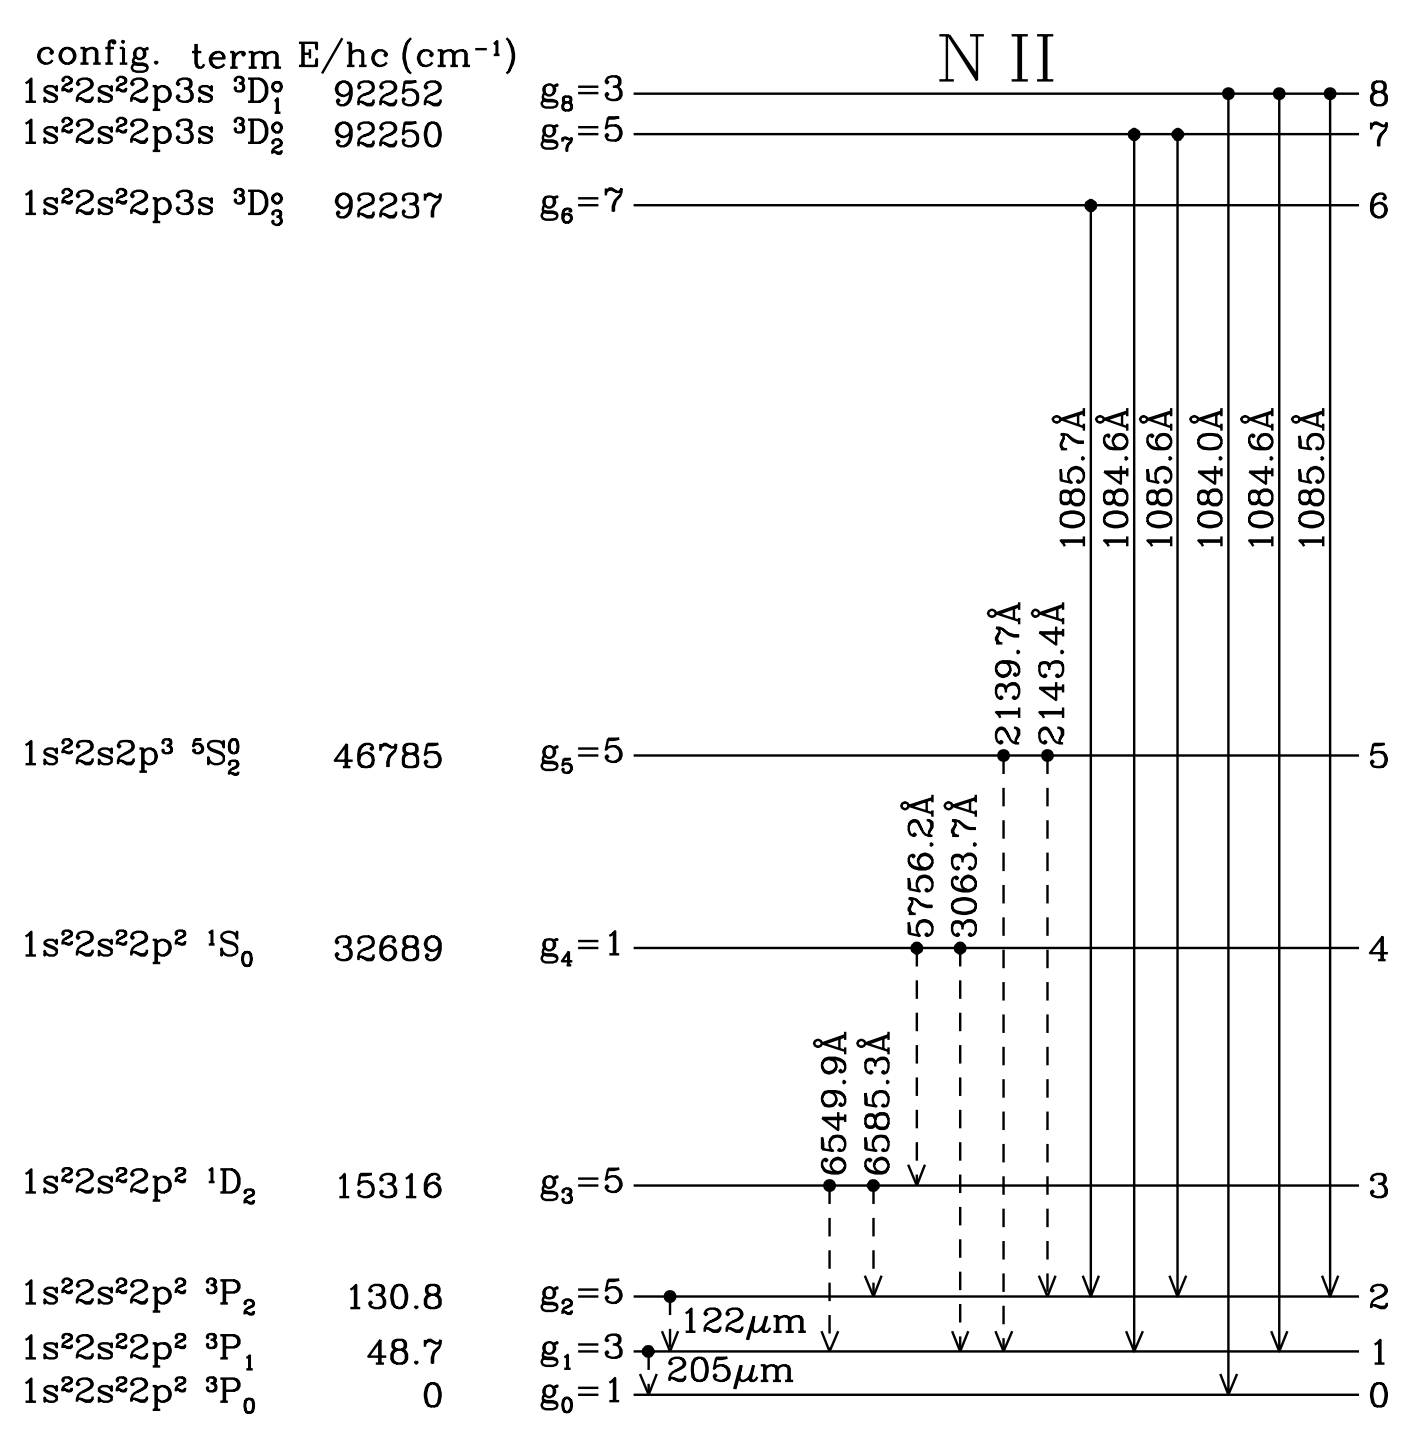
\includegraphics[width=12cm]{figures/NII_levels.png}
    \caption{\footnotesize{First nine energy levels of NII. Forbidden transitions are indicated by broken lines, and allowed transitions by solid lines; forbidden decays are not shown from levels that have permitted decay channels. Fine-structure splitting is not to scale. Hyperfine splitting is not shown. Figure taken from Draine (2015).}}
    \label{fig:NIIlevels}
\end{figure}

{\noindent}\textbf{Allowed: Electric dipole transitions:} The strongest transitions are electric dipole transitions. These are transitions satisfying the following selection rules:

\begin{enumerate}
    \item Parity must change.
    \item $\Delta L = 0, \pm1$.
    \item $\Delta J = 0, \pm1$, but $\Delta J = 0\rightarrow0$ is forbidden.
    \item Only one single-electron wave function $n\ell$ changes, with $\Delta\ell=\pm1$.
    \item $\Delta S=0$: Spin does not change.
\end{enumerate}

{\noindent}An allowed transition is denoted \textit{without} square brackets, for example,

\begin{align*}
    {\rm NII}\,1084.0{\rm \AA}\,^3P_0-^3D_1^o.
\end{align*}

{\noindent}This is a transition between the $\ell=1s^22s^22p^2\,3P_0$ and $u=1s^22s^22p3s\,^3D_1^o$ levels of NII, with a wavelength $\lambda_{u\ell}=1084.0$\,\AA. The transition has $A_{u\ell}=2.18\times10^8\,{s^{-1}}$. This decay is very fast -- the lifetime of the $^3D_1^o$ level against this decay is only $1/A_{u\ell}=4.6\,{\rm ns}$!

{\noindent}\textbf{Spin-Forbidden or inter-system transitions:} These are transitions that fulfill the electric dipole selection rules $1$ to $4$ but have $\Delta S\neq0$. These transitions are considerably weaker than allowed transitions. Such transitions are sometimes referred to as \textbf{semi-forbidden}, or \textbf{inter-combination}, or \textbf{inter-system transitions}; the latter is the terminology that we will use. An inter-system transition is denoted with a single right bracket -- for example,

\begin{align*}
    {\rm NII]}\,2143.4{\rm \AA}\,^3P_2-^5S_2^o.
\end{align*}

{\noindent}This is a transition between the $\ell=1s^22s^22p^2\,3P_2$ and $u=1s^22s2p^3\,^5S_2^o$ levels of NII, with a wavelength $\lambda_{u\ell}=2143.4$\,\AA\,and $A_{u\ell}=1.27\times10^2\,{\rm s^{-1}}$.

{\noindent}\textbf{Forbidden transitions:} Forbidden transitions are those that fail to fulfill at least one of the selection rules $1$ to $4$. The transition probabilities vary widely, depending on the values of the electric quadrupole or magnetic dipole matrix elements between the upper and lower states. A forbidden transition is denoted with two square brackets -- for example,

\begin{align*}
    {\rm [NII]}\,6549.9{\rm \AA}\,^3P_1-^1D_2^o.
\end{align*}

{\noindent}This is a transition between the $\ell=1s^22s^22p^2\,3P_1$ and $u=1s^22s^22p^2\,^1D_2^o$ levels of NII, with a wavelength $\lambda_{u\ell}=6549.9$\,\AA\,and $A_{u\ell}=9.20\times10^{-4}\,{\rm s^{-1}}$. This fails rule $1$ (parity is unchanged) and it fails rule $4$ (single electron wave functions are unchanged). This is an example of a \textbf{magnetic dipole transition}.

{\noindent}Another example of a forbidden transition is the \textbf{electric quadrupole transition}

\begin{align*}
    {\rm [NII]}\,5756.2{\rm \AA}\,^1D_2-^1S_0^o.
\end{align*}

{\noindent}This is a transition between the $\ell=1s^22s^22p^2\,1D_2$ and $u=1s^22s^22p^2\,^1S_0^o$ levels of NII, with a wavelength $\lambda_{u\ell}=5756.2$\,\AA\,and $A_{u\ell}=1.17\,{\rm s^{-1}}$. This fails rules $1$ (parity is unchanged) and $4$ (single electron wave functions are unchanged) and it fails rules $2$ and $3$ ($\Delta L=-2$ and $\Delta J=-2$), yet its transition probability is three orders of magnitude larger than the magnetic dipole transition [NII]\,$6549.9$\AA!

{\noindent}We see then that there is a hierarchy in the transition probabilities: very roughly speaking, inter-system lines are $\sim10^6$ times weaker than permitted transitions, and forbidden lines are $\sim10^2-10^6$ times weaker than inter-system transitions.

{\noindent}Despite being very ``weak,'' forbidden transitions are important in astrophysics for the simple reason that every atom and ion has excited states that can only decay via forbidden transitions. At high densities, such excited states would be depopulated by collisions, but at the very low densities of interstellar space, collisions are sufficiently infrequent that there is time for forbidden radiative transitions to take place.

\subsubsection{Follow-up Questions}

\begin{itemize}
    \item Why aren't emission and absorption lines delta functions?
    \item How does this relate to population levels and excitation temperatures?
    \item Are there emission lines in the Sun? Why is there emission from the Calcium doublet?
    \item Write down the heat transfer equation. What do solutions look like?
\end{itemize}

% --------------------------------------------------------------
%               4. 
% --------------------------------------------------------------

\newpage
\subsection{Question 4}

Describe these important sources of stellar opacity: electron scattering, free-free, bound-free, and the H$^-$ ion.

\subsubsection{Short answer}

\begin{itemize}
    \item \textbf{Electron scattering}: Also know as Thomson scattering. When an EM wave passes by an electron, the radiation field makes the electron oscillate and emit dipole radiation in all directions. This process has a small interaction cross section, so it dominates at high electron densities when the temperature is high (e.g., stellar interiors).
    \item \textbf{Free-free}: A free electron in the vicinity of an ion (which is necessary to conserve energy and momentum) will absorb a photon which results in an increased energy and momentum of the electron. This process is a source of continuum absorption.
    \item \textbf{Bound-free}: Also known as photoionization. This occurs when an atom absorbs a photon that exceeds its ionization energy and becomes ionized, resulting in a free electron that takes away any excess energy. This process is a source of continuum absorption.
    \item \textbf{H$^-$ ion}: A second electron can become loosely bound to atomic hydrogen resulting in a negatively charged ion.
\end{itemize}

\subsubsection{Additional context}

{\noindent}\textbf{Electron scattering:} If an EM wave passes an electron, the electric field makes the electron oscillate. The oscillating electron represents a classical dipole that radiates in other directions, (i.e., the electron scatters part of the energy of the incoming wave). The weakening of the original radiation due to scattering is equivalent to that by absorption, and we can describe it by way of a cross section at frequency $\nu$ per unit mass ($\kappa_\nu$). This can be calculated classically giving the result

\begin{align*}
    \kappa_\nu = \frac{8\pi}{3} \frac{e_e^2}{\mu_em_u} = 0.20(1+X) ~ [{\rm cm^2\,g^{-1}}],
\end{align*}

{\noindent}where $r_e$ is the classical electron radius, $X$ the mass fraction of hydrogen, and the constant is in ${\rm cm^2\,g^{-1}}$. The term $\mu_em_u$ arises because $\kappa_\nu$ is taken per unit mass; and $\mu_e$ is replaced by (4.30). Since $\kappa_\nu$ does not depend on the frequency, we immediately obtain the \textbf{Rosseland mean for electron scattering}:

\begin{align*}
    \kappa_{\rm sc} = 0.20(1+X) ~ [{\rm cm^2\,g^{-1}}].
\end{align*}

{\noindent}The Thomson scattering just described neglects the exchange of momentum between electron and radiation. If this becomes important, then $\kappa_\nu$ will be reduced compared to the value given above, though this effect plays a role only at temperatures sufficiently high for the scattered photons to be very energetic. In fact, during the scattering process the electron must obtain such a large momentum that its velocity is comparable to $c$, say $v\gtrsim0.1c$ for the equation above to become a bad approximation. The momentum of the photon is $h\nu/c$, which after scattering is partly transferred to the electron, $m_ev\sim h\nu/c$. Therefore relativistic corrections (\textbf{Compton scattering}) become important if the average energy of the photons is $h\nu\gtrsim0.1\,m_ec^2$. For $h\nu$ we take the frequency at which the Planck function has a maximum; then according to Wien's law this is at $h\nu=4.965\,k_BT$, and the full Compton scattering cross section has to be taken into account if $T>0.1\,m_ec^2/(4.965\,{\rm K})$, or roughly $T>10^8\,{\rm K}$. In fact even at $T=10^8\,{\rm K}$ Compton scattering reduces the opacity by only 20\% of that given by the equation above.

{\noindent}\textbf{Free-free:} If during its thermal motion a free electron passes an ion, the two charged particles form a system which can absorb and emit radiation. This mechanism is only effective as long as the electron and ion are sufficiently close. Now, the mean thermal velocity of the electrons is $v\sim\sqrt{T}$, and the time during which they form a system able to absorb or emit is proportional to $1/v\sim1/\sqrt{T}$; therefore, if in a mass element the numbers of electrons and ions are fixed, the number of systems temporarily able to absorb is proportional to $1/\sqrt{T}$.

{\noindent}The absorption properties of such a system have been derived classically; the absorption coefficient per system is proportional to $Z^2\nu^{-3}$, where $Z$ is the charge number of the ion. We therefore expect the absorption coefficient $\kappa_\nu$ of a given mixture of (fully ionized) matter to be

\begin{align*}
    \kappa_\nu \sim Z^2\rho T^{-1/2}\nu^{-3} ~ [{\rm cm^2\,g^{-1}}].
\end{align*}

{\noindent}Here the factor $\rho$ appears because for a given mass element the probability that two particles are accidentally close together is proportional to the density.

{\noindent}For the determination of the Rosseland mean $\kappa$ of this absorption coefficient we make use of a simple theorem: a factor $\nu^\alpha$ contained in $\kappa_\nu$ gives a factor $T^\alpha$ in $\kappa$. With this and the above equation for $\kappa_\nu$ we find

\begin{align*}
    \kappa_{\rm ff} \sim \rho T^{-7/2} ~ [{\rm cm^2\,g^{-1}}].
\end{align*}

{\noindent}All opacities of this form are called \textbf{Kramers opacities} and give only a classical approximation. One normally multiplies the Kramers formula by a correction factor $g$, the so-called \textbf{Gaunt factor}, in order to take care of the quantum-mechanical correction. In the equation for $\kappa_{ff}$, we have still omitted the factor $Z^2$ which appears in $\kappa_\nu$. In general, one has a mixture of different ions, and therefore one has to add the contributions of the different chemical species. The (weighted) sum over the values of $Z^2$ is taken into the constant of proportionality in $\kappa_{ff}$, which then depends on the chemical composition. For a fully ionized mixture a good approximation is given by

\begin{align*}
    \kappa_{ff} = 3.8\times10^{22} (1+X)[(X+Y)+B]\rho T^{-7/2} ~ [{\rm cm^2\,g^{-1}}],
\end{align*}

{\noindent}with the numerical constant in cgs. The mass fractions of H and He are $X$ and $Y$, respectively. Here the factor $(1+X)$ arises, since $\nu_{ff}$ must be proportional to the electron density which is proportional to $(1+X)\rho$. The term $(X+Y)$ in the brackets can be understood in the following way: there are $X/m_u$ hydrogen ions and $Y/(4m_u)$ helium ions. The former have the charge number $1$, the latter the charge number $2$. But since  $\kappa_\nu\sim Z^2$, when adding the contributions of H and He to the total absorption coefficient, we obtain the factor $X/m_u+4Y/(4m_u) = (X_Y)m_u$. Correspondingly the term $B$ gives the contribution of the heavier elements:

\begin{align*}
    B = \sum_i \frac{X_iZ_i^2}{A_i} ~ [{\rm dimensionless}],
\end{align*}

{\noindent}where the summation extends over all elements higher than helium and $A_i$ is the atomic mass number.

{\noindent}\textbf{Bound-free:} We first consider a (neutral) hydrogen atom in its ground state, with an ionization energy of $\chi_0$ (i.e., a photon of energy $h\nu>X_0$ can ionize the atom). Energy conservation then demands that 

\begin{align*}
    h\nu = \chi_0 + \frac{1}{2}m_ev_e^2 ~ [{\rm eV}],
\end{align*}

{\noindent}where $v_e$ is the velocity of the electron released (relative to the ion, which is assumed to be at rest before and after ionization). 

{\noindent}If we define an absorption coefficient $a_\nu$ per ion ($a_\nu=\kappa_\nu\rho/n_{\rm ion}$), we expect $a_\nu=0$ for $\nu<\chi_0/h$ and $a_\nu>0$ for $\nu\geq\chi_0/h$. Classical considerations similar to those which lead to the Kramers dependence of $\kappa_\nu$ for free–free transitions give a $a_\nu\sim\nu^{-3}$ for $\nu\geq\chi_0/h$. Quantum-mechanical corrections can again be taken into account by a Gaunt factor. But if we have neutral hydrogen atoms in different stages of excitation, the situation is different: an atom in the first excited stage has an absorption coefficient $a_\nu=0$ for $h\nu<\chi_1$, where $\chi_1$ is the energy necessary to ionize a hydrogen atom from the first excited state, while $a_\nu\sim\nu^{-3}$ for $h\nu\geq\chi_1$. The absorption coefficient $\kappa_\nu$ for a mixture of hydrogen atoms in different states of excitation is a superposition of the $a_\nu$ for different stages of excitation. The resulting $\kappa_\nu$ is a saw-tooth function. In order to obtain $\kappa_\nu$ for a certain value of the temperature $T$, one has to determine the relative numbers of atoms in the different stages of excitation by the Boltzmann formula; then their absorption coefficients $a_\nu$, weighted with their relative abundances, are to be summed.

{\noindent}If there are ions of different chemical species with different degrees of ionization, one has to sum the functions $a_\nu$ for all species in all stages of excitation and all degrees of ionization before carrying out the Rosseland integration. An important source of opacity are bound-free transitions of neutral hydrogen atoms, in which case the opacity must be proportional to the number of neutral hydrogen atoms and $\kappa$ can be written in the form

\begin{align*}
    \kappa_{bf} = X(1-x)\tilde{\kappa}(T) ~ [{\rm cm^2\,g^{-1}}].
\end{align*}

{\noindent}Here $\tilde{\kappa}(T)$ is obtained by Rosseland integration over (weighted) sums of functions $a_\nu$ for the different stages of excitation, while $x$ is the degree of ionization.

{\noindent}\textbf{H$^-$ ion:} Hydrogen atom has a bound state for a second electron in the field of the proton, though it has a very low ionization potential, $E_{{\rm H}^-}=0.75\,{\rm eV}$. The number density of negative hydrogen ions will be proportional to the electron density, which, in all but the most metal-poor stars, will be set by ionization of the metals (which have much lower ionization potentials that hydrogen and helium). Thus, the H$^-$ opacity will scale as $\kappa_{{\rm H}^-} \propto \rho XZ$ at low temperatures; H$^-$ is of course easily ionized at higher temperatures, and at very low temperatures even metals will not be ionized, so there will be no electrons to form H$^-$ by combining with H.

% --------------------------------------------------------------
%               5. 
% --------------------------------------------------------------

\newpage
\subsection{Question 5}

Describe the processes that can cause pulsations in a star's luminosity, and provide at least one example of a class of stellar pulsation.

\subsubsection{Short answer}

Stellar pulsations can occur when a star's surface is expanding and contracting which causes its surface area, and thus luminosity, to vary: $L=4\pi R^2\sigma T^4$. Radial oscillations of a pulsating star, for example, are the result of sound waves resonating in the star's interior. For such radial oscillations, displacement of stellar material occurs primarily on the surface. A star has an infinite number of modes of radial pulsation.  The simplest is called the fundamental mode. In this mode, all parts of the star expand together and contract together in unison. The next simplest mode is the first overtone. In this mode, there is a nodal sphere in the star where the material remains at rest. When the part of the star outside this sphere is expanding, the part inside is contracting, and vice versa. In the second overtone mode, there are two nodal spheres, where the material remains at rest.  The large-amplitude pulsating stars (Cepheids, RR Lyrae variables, and Mira variables) pulsate primarily in radial modes.

\subsubsection{Additional context}

{\noindent}For a star to begin and continue to pulsate, there must be some mechanism which converts radiant energy into energy of motion in a timely way, overcoming friction and building up the motion. Such a mechanism can exist in a star: it is the thermodynamic effect of an ionization zone in a star. In a star of moderate surface temperature, the layers below the surface have temperatures up to a few tens of thousands of degrees. The helium tends to be singly-ionized; it has lost one of its two electrons but not the second. If the star contracts, it heats slightly which causes the helium to lose its second electron. This requires energy which comes from the radiation flowing outward through the gas; it is absorbed by the opacity of the gas. The energy then becomes stored in the form of ionization energy. When the star subsequently expands and cools, the electrons recombine with the helium atoms, and release the stored-up ionization energy. This is the `push' which maintains the pulsation in all of the pulsating stars in the Cepheid instability strip.

{\noindent}\textbf{CHAPTER 14 OF CARROLL AND OSTLIE}.

{\noindent}Variable stars are stars which change in brightness. The change may be as small as a few parts in a million, or it may be a factor of a thousand or more. It may occur in a second or less, or it may take years, decades, or centuries. These are extremes, but astronomers have developed an array of techniques for discovering, measuring, and analyzing the full range of possible variable stars. Why? Because the variations provide important and often unique information about the nature and evolution of the stars. This information can be used to deduce even more fundamental knowledge about our universe in general.

{\noindent}The variations may be due to the rotation of a spotted star, or to an eclipse of a star by a companion star, or even by an unseen planet. The variations may be due to the vibrations of a star; if they are complex enough (as they are in our Sun), they may provide an internal `picture' of the star. The variations may be due to eruptions on a star (flares), an accretion disc (dwarf novae), major explosions on a star (novae), or to the total disruption of a star in a supernova. SNe are the most violent events in our Universe, yet we owe our existence to them, because they help to recycle the atoms, created in stars, into space where some of them became part of our Sun, our planet, and our biosphere. Also, the elements heavier than iron were mostly created in SNe explosions. SNe may be dramatic and extreme, but they represent only one of the many roles that variable stars play in modern astrophysics, and in our understanding of the Universe and the processes which govern it.

{\noindent}\textbf{Classification of variable stars}: The earliest classification scheme dates back nearly two centuries: Pigott divided variables according to the nature of their light curve into novae, long- period variables, and short-period variables. A century later, Pickering devised a more detailed scheme: (la) normal novae, primarily nearby ones in our own galaxy; (lb) novae in nebulae: now known to be primarily SNe in distant galaxies; (IIa) long-period variables, cool, large-amplitude pulsating variables; (IIb) U Geminorum stars, dwarf novae; (IIc) R Coronae Borealis stars, stars which suddenly and unpredictably decline in brightness; (III) irregular variables, a motley collection; (IVa) short-period variables, such as Cepheids and later including the cluster-type or RR Lyrae stars; (IVb) Beta Lyrae type eclipsing variables; and (V) Algol type eclipsing variables.

{\noindent}Pickering's classification scheme contains some hints as to the nature and cause of the variability. Classification and explanation go hand in hand (in principle), and in the late nineteenth and early twentieth centuries, progress was made in understanding the physical nature and the physical processes in variable stars, and in stars in general.

{\noindent}\textbf{Pulsating variable stars}: Pulsation is the astronomer's word for \textit{vibration or oscillation}. Every physical object has natural patterns or modes of vibration, each with a corresponding period -- the time required for one vibration.

{\noindent}\textbf{Pulsation modes}: Stars are, to a first approximation, spherical. The simplest form of pulsation is radial pulsation -- a simple, spherically symmetric in-and-out expansion and contraction. A star has an infinite number of modes of radial pulsation. The simplest is called the \textbf{fundamental mode}. In this mode, all parts of the star expand together and contract together, in unison. The next simplest mode is the \textbf{first overtone}. In this mode, there is a nodal sphere in the star, where the material remains at rest. When the part of the star outside this sphere is expanding, the part inside is contracting, and vice versa. In the \textbf{second overtone mode}, there are two nodal spheres, where the material remains at rest. The large-amplitude pulsating stars -- \textbf{Cepheids}, \textbf{RR Lyrae variables}, and \textbf{Mira variables} -- pulsate primarily in radial modes. Radial pulsation produces substantial changes in luminosity (and therefore brightness), temperature (and therefore colour), and radial velocity; these are observed, and provide direct evidence for the radial pulsation. Through techniques such as the \textbf{Baade-Wesselink method}, they can be used to determine the average radius of the star.

{\noindent}It is less easy to tell which radial mode a star is pulsating in. Most, but not all, large-amplitude variables pulsate in the fundamental mode. If the radius and mass of the star can be estimated, the observed period can be compared with the theoretical or expected period for each mode. If the star pulsates in two or more radial modes, then the period ratio can be used to deduce the modes.

{\noindent}In \textbf{non-radial pulsations}, the star changes shape, not volume (Figure \ref{fig:nonradialpulsations}). There is a triply-infinite set of modes, corresponding to the three different co-ordinate axes on the star. These are chosen to be: the distance from the centre, the angular distance (`latitude') above or below the star's equator, and the angular distance (`longitude') around the star's equator. Non-radial modes can be divided into (i) \textbf{p (pressure) modes}, in which the motion is primarily radial and the restoring force is pressure (as it is in radial modes), and (ii) \textbf{g (gravity) modes}, in which the motion is primarily horizontal, and the restoring force is buoyancy or gravity (as it is in water waves). A wide assortment of stars pulsate non-radially. Non-radial pulsation tends to produce smaller amplitudes than radial modes in the brightness and colour variation, but, if they can be observed, their relative amplitudes and phases (along with the periods themselves) can be used to identify the precise non-radial mode. Non-radial pulsation also produces characteristic absorption line profile variations. With modern high S/R spectrographs, these can and have been observed and studied over time. Also, there are often very close non-radial periods, whose differences are a clue to the mode identification. In non-rotating stars, these close periods are actually identical or degenerate, but in a rotating star, they become different; the difference is proportional to the amount of rotation. The situation is complicated by the fact that many of these non-radially pulsating stars rotate rapidly, and the theory of rapidly rotating pulsating stars is not well understood.

\begin{figure}[t]
    \centering
    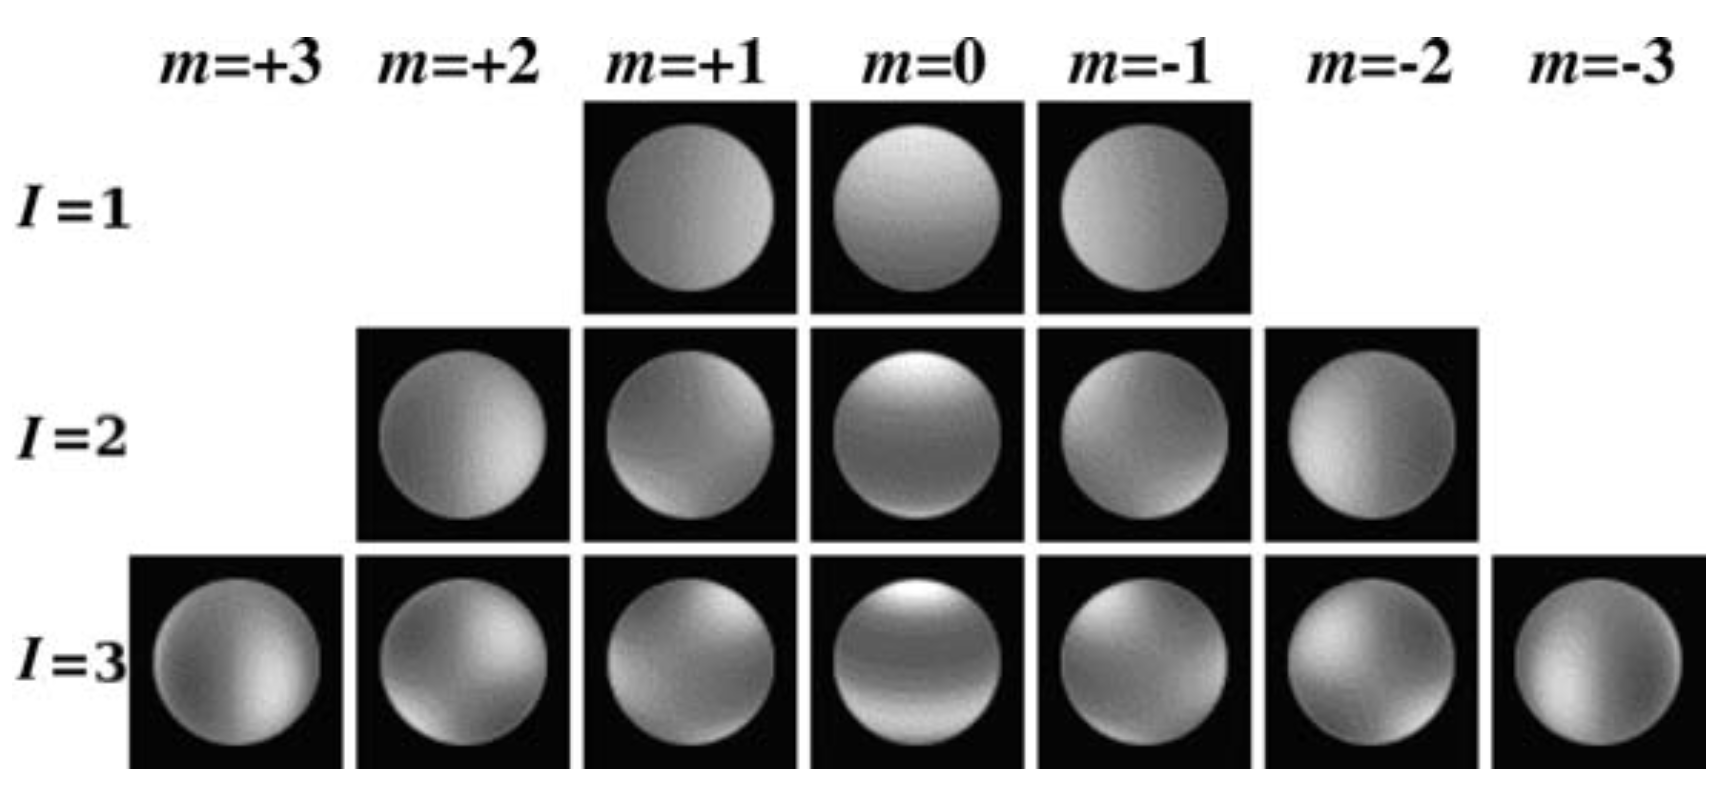
\includegraphics[width=14cm]{figures/NonradialPulsations.png}
    \caption{\footnotesize{Illustration of non-radial pulsation modes. When the light-coloured regions are moving downward, the dark-coloured regions are moving upward. In radial pulsation, all parts of the star move in and out in unison. (Source: Whole Earth Telescope). Figure taken from Percy (2007).}}
    \label{fig:nonradialpulsations}
\end{figure}

{\noindent}\textbf{Modelling stellar pulsation}: The theory of stellar pulsation begins with a model of the star which gives the physical properties of the star as a function of distance from the centre. The first models of stars were primitive (and so were the deductions from stellar pulsation theory). Now, with improved understanding of the physics of stars, and powerful computers to implement this knowledge, the models are much more detailed and accurate.

{\noindent}The simplest level of modelling is the \textbf{linear adiabatic theory} (LAT) of radial pulsation of a spherically symmetric, non-rotating, non-magnetic star. This was formulated by Arthur Eddington, early in the twentieth century. It assumes that the pulsations are infinitesimally small, and that there is no transfer of energy between parts of the star. It provides reasonable estimates of the periods of the radial modes and their dependence on the physical properties of the star. For instance, it shows that the period of any mode is approximately inversely proportional to the square root of the mean density of the star. Alternatively, the period times the square root of the density is approximately constant; we call it the \textbf{Q-value}, or \textbf{pulsation constant}. It is this relationship which leads to the period-luminosity relation; since both period and luminosity are related to the radius of the star, and since the temperatures of pulsating stars are about the same, period and luminosity will be related to each other. The LAT also shows that the relative amplitude of pulsation tends to be largest in the outer layers, where the density is lowest. Corresponding calculations can be done for non-radial pulsation. The LAT assumes that the pulsation takes the form of a standing wave in the star (i.e., a wave which is perfectly reflected from the centre and the surface).

{\noindent}The next level of complexity is the \textbf{linear non-adiabatic theory} (LNAT). This also assumes that the pulsations are infinitesimally small, but it allows for the possibility that any layer of the star may gain or lose energy. In particular, the amplitude of the infinitesimal pulsations can increase or decrease, and we can tell what modes may be unstable, and grow. We cannot tell what the eventual amplitudes may be (i.e., which mode(s) may grow to become observable). The LNAT gives periods which are slightly more realistic than the LAT, though they are about the same in most cases.

{\noindent}The next level of complexity is the \textbf{non-linear, non-adiabatic theory}, which amounts to a full, time-dependent, hydrodynamical model of the star. This includes the equation which relates the motion of a layer in the star to the forces acting on it. The calculation begins with the static, `equilibrium' model of the star. Infinitesimal random motions are imposed on the model (such as from the round-off errors in the calculations), to see if they grow or decay. After several hundred cycles, the model (usually) reaches some constant, stable amplitude in one or more modes. The non-linear theory accurately predicts the amplitudes of Cepheids and RR Lyrae stars, which pulsate in one or two radial modes. It has not been able to explain stars like Delta Scuti stars, which can and do pulsate in many radial and non-radial modes. An ongoing problem in stellar pulsation is: what determines what mode(s) a star will pulsate in, and with what amplitude?

{\noindent}These models are non-rotating and non-magnetic. Non-linear analysis of rotating magnetic models is at the frontier of present research. But we know that all stars rotate (some of them very rapidly) and that many of them have significant magnetic fields. In reality, there is no such thing as a truly spherically symmetric star; for most of them, however, that is a reasonable approximation.

{\noindent}\textbf{Non-linear effects}: The pulsation waves in a star are not reflected perfectly from the surface, but move outward in an atmosphere of decreasing density. In many variables, such as Mira stars, this creates \textbf{shock waves} as the atmospheric layers pile up against each other. In Mira stars, this creates layers of higher density where gases condense into dust. The dust absorbs the star's radiation and is pushed outward, carrying gas along with it. The result is mass loss which has a profound effect on the star and the space around it. In the largest, most luminous supergiants, the outward radiation pressure almost balances or perhaps even exceeds gravity; the star borders on instability; and non-linear effects may be significant.

{\noindent}\textbf{The instability strip(s)}: Normally, stars are stable. The inward pull of gravity is balanced by the outward pressure of the hot gas in the star. If the star begins to contract, its internal pressure and temperature increase and reverse the contraction. If the star begins to expand, its internal pressure and temperature decrease and gravity restores the initial balance. Furthermore, if a star expands or contracts, the energy of motion is dissipated by friction. Eventually the star returns to rest.

{\noindent}For a star to begin and continue to pulsate, there must be some mechanism which converts radiant energy into energy of motion in a timely way, overcoming friction and building up the motion. Such a mechanism can exist in a star: it is the thermodynamic effect of an ionization zone in a star.

{\noindent}In a star of moderate surface temperature, the layers below the surface have temperatures up to a few tens of thousands of degrees. The helium tends to be singly-ionized; it has lost one of its two electrons but not the second. If the star contracts, it heats slightly which causes the helium to lose its second electron. This requires energy which comes from the radiation flowing outward through the gas; it is absorbed by the opacity of the gas. The energy then becomes stored in the form of ionization energy. When the star subsequently expands and cools, the electrons recombine with the helium atoms, and release the stored-up ionization energy. This is the `push' which maintains the pulsation in all of the pulsating stars in the Cepheid instability strip (Figure \ref{fig:variablezones}). If there is sufficient mass in the ionization zone to store up significant radiant energy during the pulsation cycle, then the star will pulsate. This mechanism is referred to as \textbf{self-exciting}, in contrast to the pulsations of the Sun and other Sun-like stars, which are excited by the turbulence in their convection zones.

\begin{figure}[h]
    \floatbox[{\capbeside\thisfloatsetup{capbesideposition={right,top},capbesidewidth=4cm}}]{figure}[\FBwidth]
    {\caption{\footnotesize{Diagram showing the zones in an unstable star which convert radiant energy into kinetic energy, and vice versa, in a model of a pulsating RR Lyrae star, expressed as the fractional energy production (positive) or dissipation (negative) per period. The centre of the star is at the left, the atmosphere at the right. The two energizing zones (the hydrogen zone and the ionized helium (He II) zone) are shown, along with the principal dissipation zone, deeper in the star. (From Christy, 1966.) Figure taken from Percy (2007).}}
    \label{fig:variablezones}}
    {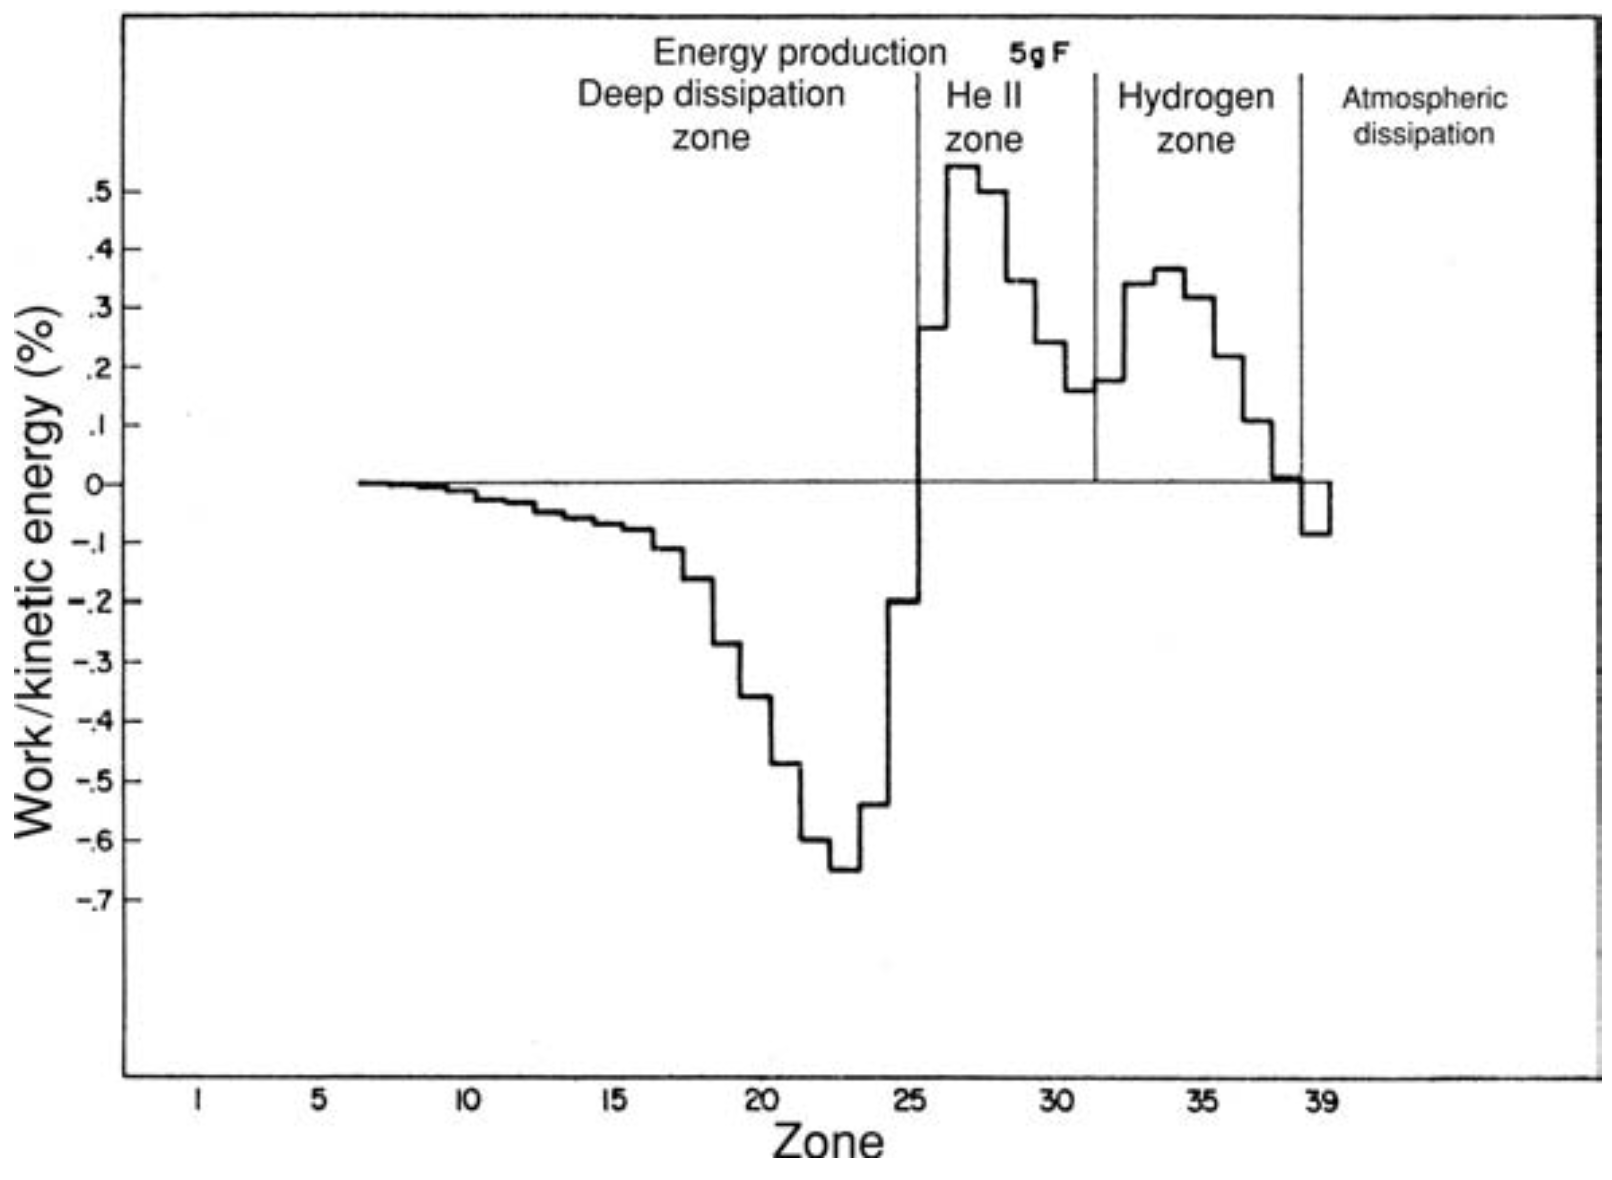
\includegraphics[width=8cm]{figures/VariableZones.png}}
\end{figure}

{\noindent}But what about the other types of pulsating stars? The Beta Cephei stars were a real mystery, because they are much hotter than the Cepheid instability strip. Only in the 1980s was it realized that the ionization of iron, at temperatures near $150,000\,{\rm K}$ deep within the star had sufficient effect to maintain the pulsation. This realization came about as a result of physicists' recalculation of the opacity of iron at these temperatures. This solved the long-standing mystery of the Beta Cephei stars, and some other nagging problems in pulsation theory as well.

{\noindent}Figure \ref{fig:hrpulsating} shows the location of various types of pulsating variable stars in the HR diagram. There is a misconception often included in astronomy textbooks that pulsation is something that happens only in evolved stars such as giants and supergiants. In fact, the Cepheid instability strip extends from the top of the HR diagram to the bottom, at approximately constant temperature. That is because the instability mechanism occurs at a particular temperature -- the temperature at which there is a helium ionization zone in the outer layers of the star. So supergiant Cepheids pulsate, main-sequence Delta Scuti stars pulsate, and white dwarfs pulsate -- all as a result of the same mechanism.

\begin{figure}[t]
    \floatbox[{\capbeside\thisfloatsetup{capbesideposition={right,top},capbesidewidth=4cm}}]{figure}[\FBwidth]
    {\caption{\footnotesize{The location of various types of pulsating star on the HR diagram. The main instability regions are the Cepheid strip, including its intersection with the main sequence (dashed line), the region of the coolest stars (Miras and their relatives), and the region of the Beta Cephei and SPB stars. There are also instability regions along the white dwarf cooling track (dotted line) at the bottom of the diagram, including the nuclei of planetary nebulae (PNNV) and the DOV, DBV, and DAV pulsating white dwarfs. (From J. Christensen-Dalsgaard, private communication.) Figure taken from Percy (2007).}}
    \label{fig:hrpulsating}}
    {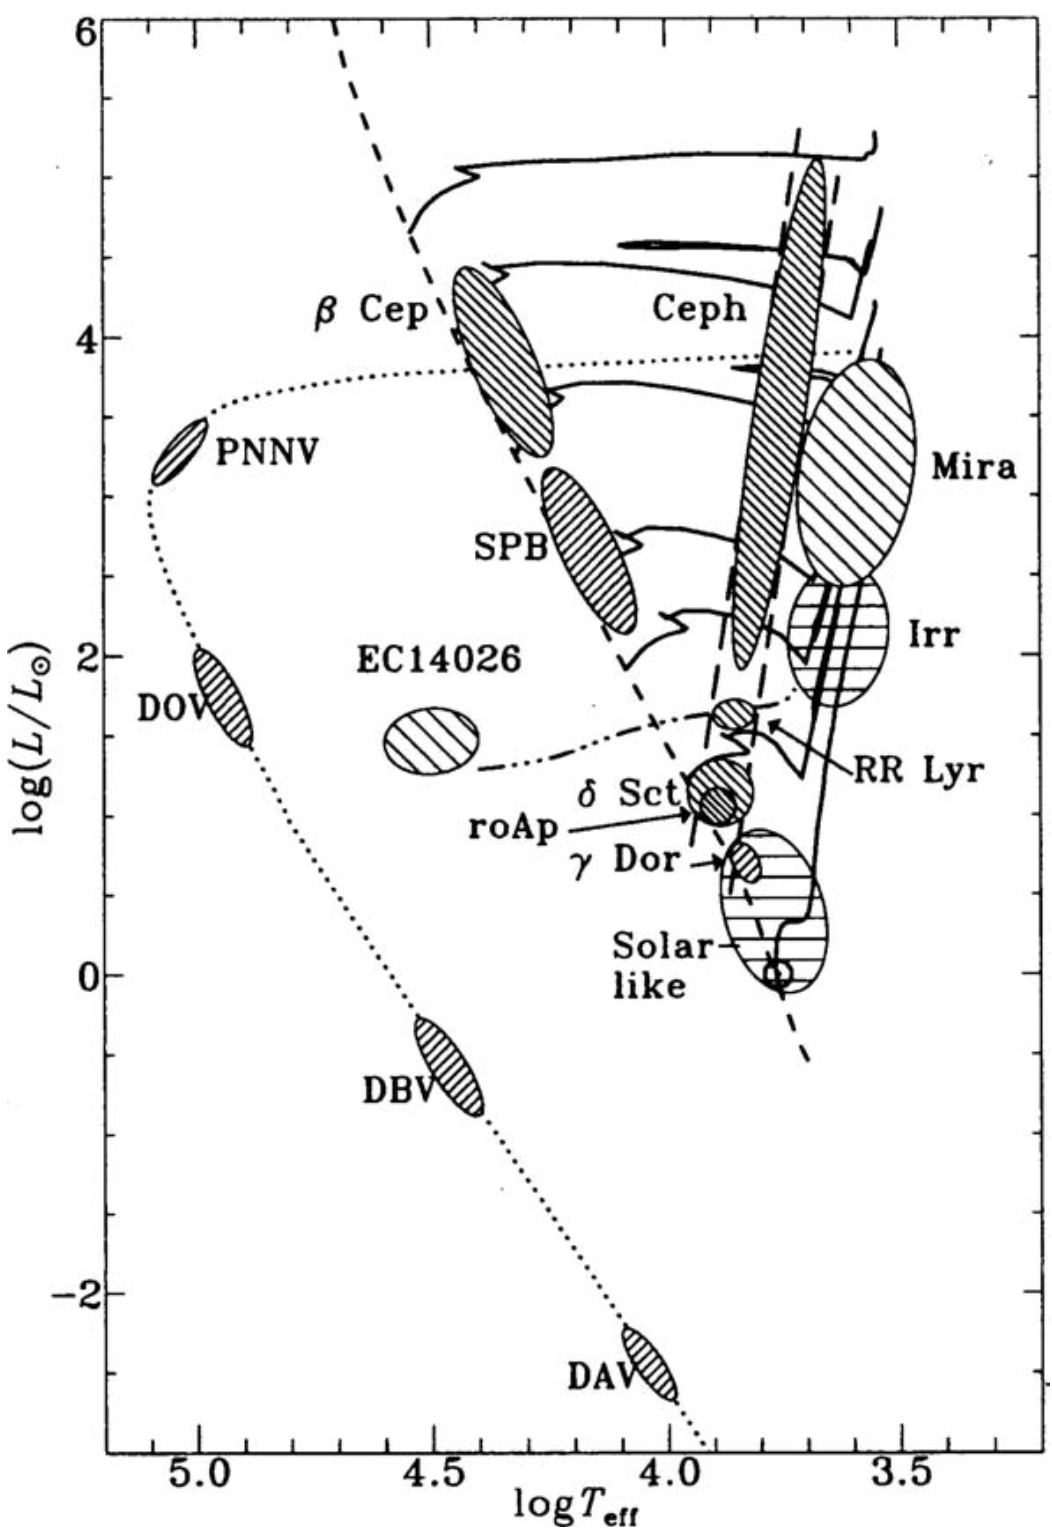
\includegraphics[width=8cm]{figures/HR_pulsating.png}}
\end{figure}

{\noindent}The Cepheid instability strip is not exactly vertical: its temperature is cooler at its high-luminosity end. That is because more luminous stars have outer regions of lower density; at lower density, ionization can occur at a lower temperature because there is lots of `room' for the electrons that are released.

{\noindent}Stars can evolve into the instability strip in different ways (figure 6.4). Massive young stars can evolve quickly from left to right in the HR diagram; old low-mass stars can evolve slowly to the same position. So there may be Population I and II stars in the same region of the instability strip.

\begin{figure}[t!]
    \floatbox[{\capbeside\thisfloatsetup{capbesideposition={right,top},capbesidewidth=4cm}}]{figure}[\FBwidth]
    {\caption{\footnotesize{Evolution tracks on the HR diagram, showing the changes which take place in a star as it evolves. The tracks are marked by the mass of the star in solar units. The Cepheid pulsation instability strip is marked IS, and the horizontal branch where RR Lyrae (RR) variables are found is marked HB. The time scales for evolution depend on the mass: the more massive the star, the faster the evolution. (From Kaler, 1997.) Figure taken from Percy (2007).}}
    \label{fig:inststripevol}}
    {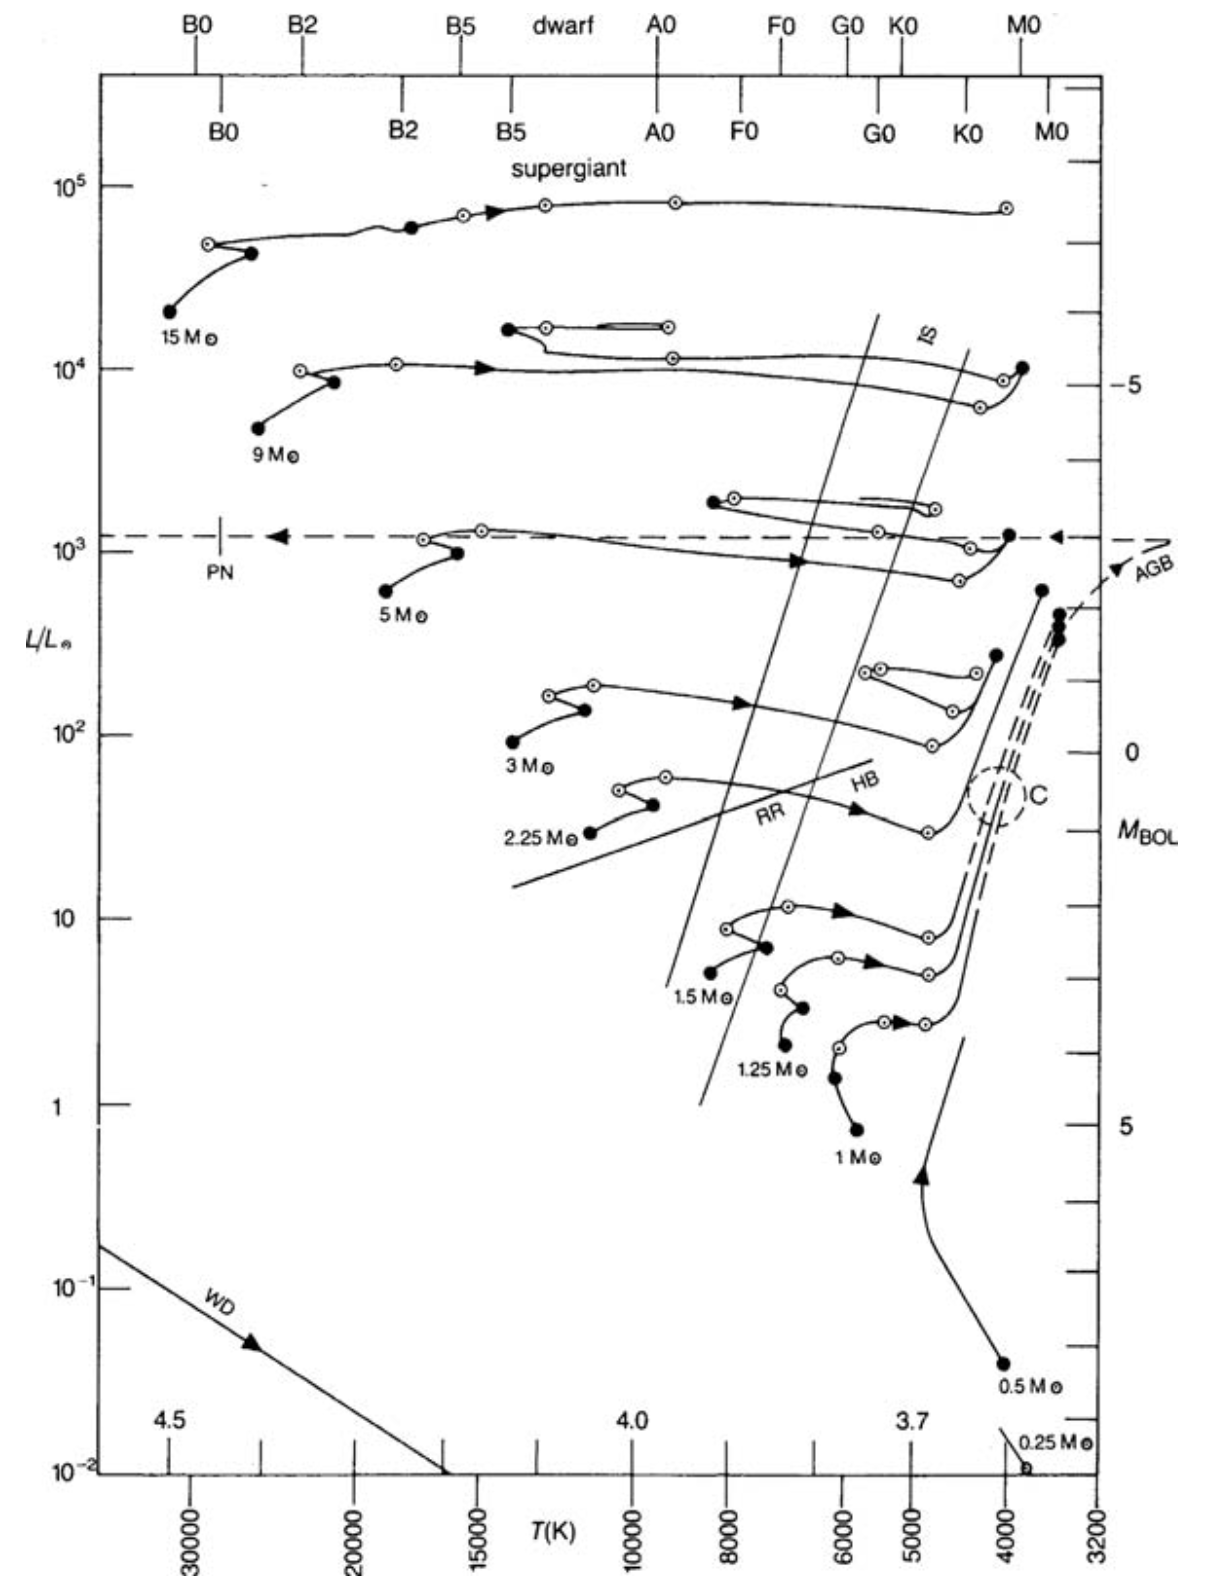
\includegraphics[width=8cm]{figures/InstStripEvol.png}}
\end{figure}

{\noindent}Stars can evolve into the instability strip in different ways (Figure \ref{fig:inststripevol}). Massive young stars can evolve quickly from left to right in the HR diagram; old low-mass stars can evolve slowly to the same position. So there may be Population I and II stars in the same region of the instability strip.

\newpage
\subsubsection{Follow-up Questions}

\begin{itemize}
    \item What about the instability strip? RR Lyrae?
    \item What is the period-luminosity relation?
    \item What is the form of the period-luminosity relation?
    \item How would you derive the time scale of pressure waves in a star?
    \item How would you order-of-magnitude estimate the period for a pulsation?
\end{itemize}

% --------------------------------------------------------------
%               6. 
% --------------------------------------------------------------

\newpage
\subsection{Question 6}

Briefly describe the sources of thermal energy for stars and planets.

\subsubsection{Short answer}

The sources of thermal energy of stars include:

\begin{itemize}
    \item \textbf{gravitational energy}: As a star contracts, gravitational potential energy can be converted into thermal energy.
    \item \textbf{rotational energy}: The gas cloud from which stars form acquire angular momentum from their environment which is conserved as the collapse, thus increasing their rotation rate.
    \item \textbf{nuclear energy}: The primary source of energy for main sequence stars. Most of the energy to be gained from nuclear fusion occurs by the conversion of hydrogen to helium and less than one half of that energy can be obtained by all other fusion processes that carry helium to iron.
\end{itemize}

{\noindent}The sources of thermal energy of planets include:

\begin{itemize}
    \item \textbf{radioactive decay}: The exothermic decay of radioactive isotopes within planet cores.
    \item \textbf{differentiation}: The separation of heavier material towards the core of a molten planet from lighter materials which float towards the surface during planet formation which converts gravitational potential to thermal energy.
    \item \textbf{solar radiation}: The incident radiation on a planet's surface from its host star can heat the surface either via absorption or the greenhouse effect.
    \item \textbf{accretion/impact}: The conversion of kinetic energy to thermal energy upon asteroids etc. hitting the surface of planets; primarily during planet formation (i.e., bombardment).
    \item \textbf{tidal heating}: Tidal heating occurs through the tidal friction processes: orbital energy is dissipated as heat in either the surface ocean or interior of a planet or satellite. When an object is in an elliptical orbit, the tidal forces acting on it are stronger near periapsis than near apoapsis.
\end{itemize}

\subsubsection{Additional context}

{\noindent}\textbf{Stars:}

{\noindent}One of the great mysteries of the late nineteenth and early twentieth centuries was the source of the energy required to sustain the luminosity of the sun. By then, the defining Solar parameters of mass, radius, and luminosity were known with sufficient precision to attempt to relate them. For instance, it was clear that if the Sun derived its energy from chemical processes typically yielding less that $10^{12}\,{\rm erg\,g^{-1}}$, it could shine no longer than about $10,000$ years at its current luminosity. It is said that Lord Kelvin, in noting that the liberation of gravitational energy could only keep the sun shining for about $10$ million years, found it necessary to reject Charles Darwin's theory of evolution because there would have been insufficient time for natural selection to provide the observed diversity of species.

{\noindent}\textbf{Gravitational energy:} It is generally conceded that the Sun has shone at roughly its present luminosity for at least the past $2$ billion years and has been in existence for nearly $5$ billion years. With this in mind, let us begin our study of the sources of stellar energy with an inventory of the stores of energy available to the sun. Perhaps the most obvious source of energy is that suggested by Lord Kelvin, namely gravitation:

\begin{align*}
    E_p \leq -\frac{3}{5}\frac{GM^2}{R} ~ [{\rm J}].
\end{align*}

{\noindent}The right-hand side of the inequality is the gravitational potential energy for a uniform density sphere, which provides a sensible upper limit for the energy. Remember that the gravitational energy is considered negative by convention; a rather larger magnitude of energy may be available for a star that is more centrally concentrated than a uniform-density sphere. We may acquire a better estimate of the gravitational potential energy by using the results for a polytrope. Chandrasekhar obtains the following result for the gravitational potential energy of a polytrope:

\begin{align*}
    E_p = -\frac{3}{5-n}\frac{GM^2}{R} ~ [{\rm J}].
\end{align*}

{\noindent}For a star in convective equilibrium (that is, $n=3/2$) the factor multiplying $GM^2/R$ becomes $6/7$ or nearly unity. Note that for a polytrope of index $5$, $U_g\rightarrow-\infty$ implying an infinite central concentration of material. This is also one of the polytropes for which there exists an analytic solution. Thus, one has the picture of a mass point surrounded by a massless envelope of infinite extent. This equation also tells us that as the polytropic index increases, so does the central concentration.

{\noindent}It is not at all obvious that the total gravitational energy would be available to permit the star to shine. Some energy must be provided in the form of heat, to provide the pressure which supports the star. We may use the Virial theorem [equation (1.2.35)] to estimate how much of the gravitational energy can be utilized by the luminosity. Consider a star with no mass motions, so that the macroscopic kinetic energy T in equation (1.2.35) is zero. Let us also assume that the equilibrium state is good enough that we can replace the time averages by the instantaneous values. Then the \textbf{Virial theorem becomes}

\begin{align*}
    2E_k+E_p = 0 ~ [{\rm J}].
\end{align*}

{\noindent}Recall that $E_k$ is the total internal kinetic energy of the gas which includes all motions of the particles making up the gas. Now we know from thermodynamics that not all the internal kinetic energy is available to do work, and it is therefore not counted in the internal energy of the gas.

{\noindent}For simplicity, let us assume that $\gamma$ is constant through out the star. Remembering that the total energy $E$ is the sum of the internal energy and the gravitational energy, we can express the Virial theorem in the following ways:

\begin{align*}
    E_k &= -\frac{E_p}{3(\gamma-1)} ~ [{\rm J}]\\
    E_{\rm tot} &= -(3\gamma-4)E_{\rm th} ~ [{\rm J}]\\
    E_{\rm tot} &= \frac{3\gamma-4}{3(\gamma-1)}E_p ~ [{\rm J}].
\end{align*}

{\noindent}It is clear that for $\gamma>4/3$ (that is, $n<3$), the total energy of the star will be negative. This simply says that the star is gravitationally bound and can be in equilibrium. So we can look for the physically reasonable polytropes to have indices less than or equal to $3$. The case of $n=3$ is an interesting one for it represents radiation dominated gas. In the limit of complete radiation dominance, the total energy of the configuration will be zero.

{\noindent}\textbf{Rotational energy:} Stars do rotate, and we should not forget to count the rotational energy in the inventory of energies. We may place a reasonable upper limit on the magnitude of the rotational energy that we can expect by noting that (1) the moment of inertia of the star will always be less than that of a sphere of uniform density and (2) there is a limit to the angular velocity $\omega_c$ at which the star can rotate. Thus, for a centrally condensed star

\begin{align*}
    \omega^2 &= \frac{8GM}{27R^3} ~ [{\rm km^2\,s^{-2}\,kpc^{-2}}] \\
    I_z &< \frac{2}{5}MR^2 ~ [{\rm kg\,km^2}],
\end{align*}

{\noindent}which implies that the rotational energy must be bounded by

\begin{align*}
    E_{\rm rot} = \frac{1}{2}I_z\omega^2 < \frac{8}{135}\frac{GM^2}{R} ~ [{\rm J}].
\end{align*}

{\noindent}One may quibble that we have used the angular velocity limit for a centrally condensed star and the moment of inertia for a uniform-density star, but the fact remains that it is extremely difficult for a star to have more than about 10 percent of the magnitude of its gravitational energy stored in the form of rotational energy.

{\noindent}\textbf{Nuclear energy:} Of course, the ultimate upper limit for stored energy is the energy associated with the rest mass itself. It is also the common way of estimating the energy available from nuclear sources. Indeed, that fraction of the rest mass which becomes energy when four hydrogen atoms are converted to one helium atom provides the energy to sustain the solar luminosity. Below in Table \ref{table:solarenergy} is a short table giving the mass loss for a few common elements involved in nuclear fusion processes.

\begin{table}[h]
    \centering
    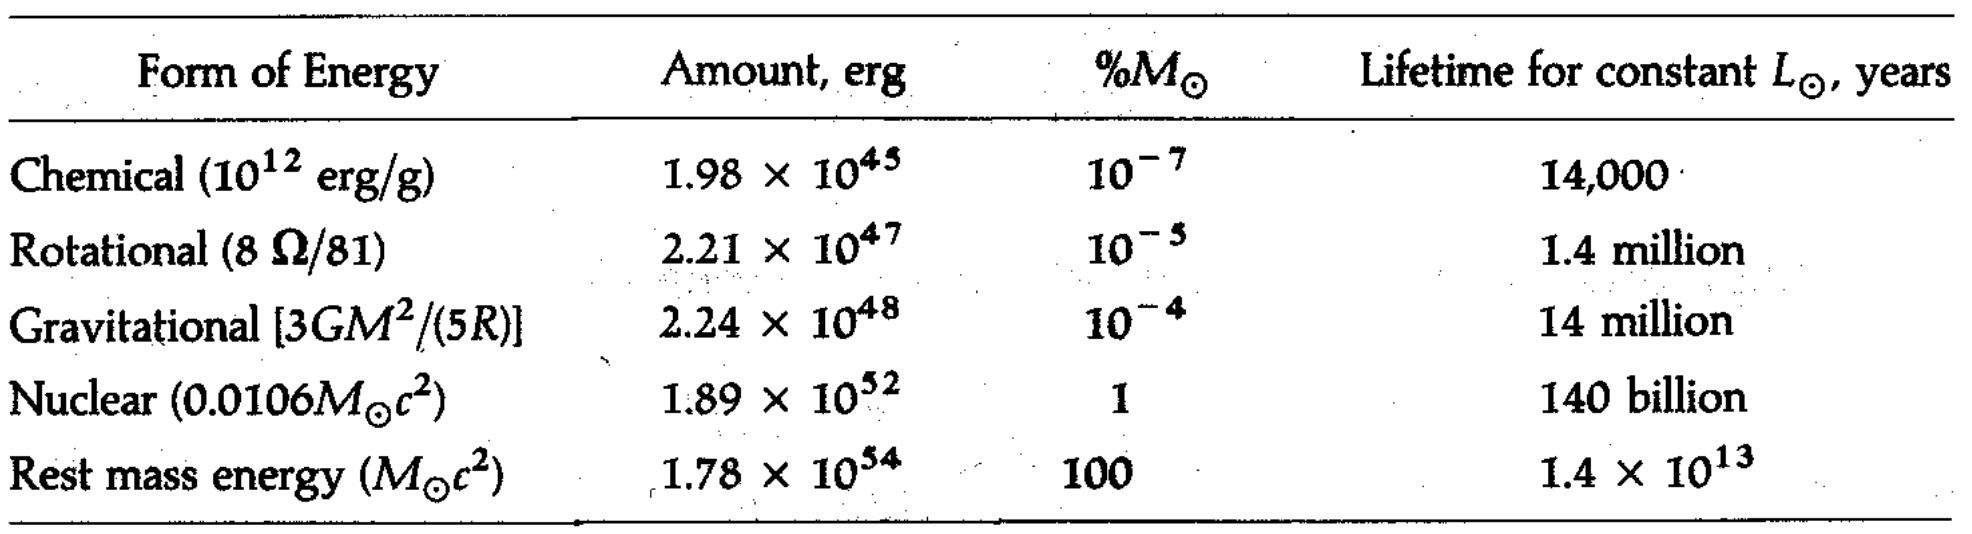
\includegraphics[width=14cm]{figures/SolarEnergy.png}
    \caption{\footnotesize{Possible sources of Solar energy. Table taken from Kippenhahn, Weigert \& Weiss (2012).}}
    \label{table:solarenergy}
\end{table}

{\noindent}Clearly most of the energy to be gained from nuclear fusion occurs by the conversion of hydrogen to helium and less than one-half of that energy can be obtained by all other fusion processes that carry helium to iron. Nevertheless, $0.7\%$ of $mc^2$ is a formidable supply of energy. Table \ref{table:solarenergy} is a summary of the energy that one could consider as being available to the Sun. All these entries are generous upper limits. For example, the sun rotates at less than $0.5\%$ of its critical velocity, it was never composed of $100\%$ hydrogen and will begin to change significantly when a fraction of the core hydrogen is consumed, and not all the gravitational energy could ever be converted to energy for release. In any event, only nuclear processes hold the promise of providing the solar luminosity for the time required to bring about agreement with the age of the solar system as derived from rocks and meteorites. However, the time scales of Table \ref{table:solarenergy} are interesting because they provide an estimate of how long the various energy sources could be expected to maintain some sort of equilibrium configuration.

{\noindent}\textbf{Planets:}

\subsubsection{Follow-up Questions}

\begin{itemize}
    \item Why do different nuclear reaction pathways have different temperature sensitivities?
    \item If I assume a constant core temperature on the main sequence, how does stellar radius depend on mass?
    \item What are some other thermal sources, like say for neutron stars?
\end{itemize}

% --------------------------------------------------------------
%               7. 
% --------------------------------------------------------------

\newpage
\subsection{Question 7}

Describe the process by which supernovae produce light. Why are Type Ia supernovae generally brighter than Type II events?

\subsubsection{Short answer}

\begin{itemize}
    \item \textbf{Type Ia SNe}: 
    \item \textbf{Type II (core-collapse) SNe}: 
\end{itemize}

\subsubsection{Additional context}

{\noindent}\textbf{Classification of supernovae}: Based on their spectral properties, SNe are divided into several classes. SNe of Type I do not show any Balmer lines of hydrogen in their spectrum, in contrast to those of Type II. The Type I SNe are further subdivided: SNe Ia show strong emission of SiII $\lambda\,6150$\AA~whereas no SiII at all is visible in spectra of Type Ib,c. Our current understanding of the supernova phenomenon differs from this spectral classification.\footnote{This notation scheme (Type Ia, Type II, and so on) is characteristic for phenomena that one wishes to classify upon discovery, but for which no physical interpretation is available at that time. Other examples are the spectral classes of stars which are not named in alphabetical order nor according to their mass on the main sequence; or the division of Seyfert galaxies into Type 1 and Type 2. Once such a notation is established, it often becomes permanent even if a later physical understanding of the phenomenon suggests a more meaningful classification.} Following various observational results and also theoretical analyses, we are confident today that SNe Ia are a phenomenon which is intrinsically different from the other supernova types. For this interpretation, it is of particular importance that SNe Ia are found in all types of galaxies, whereas we observe SNe II and SNe Ib,c only in spiral and irregular galaxies, and here only in those regions in which blue stars predominate. The stellar population in elliptical galaxies consists almost exclusively of old stars, while spirals also contain young stars. From this observational fact it is concluded that the phenomenon of SNe II and SNe Ib,c is linked to a young stellar population, whereas SNe Ia occur also in older stellar populations.

{\noindent}\textbf{Core-collapse supernovae}: SNe II and SNe Ib,c are the final stages in the evolution of massive ($\gtrsim8\,{\rm M}_\odot$) stars. Inside these stars, ever heavier elements are generated by nuclear fusion: once all the hydrogen in the inner region is used up, helium will be burned, then carbon, oxygen, etc. This chain comes to an end when the iron nucleus is reached, the atomic nucleus with the highest binding energy per nucleon. After this no more energy can be gained from fusion to heavier elements so that the pressure, which is normally balancing the gravitational force in the star, can no longer be maintained. The star then collapse under its own gravity. This gravitational collapse proceeds until the innermost region reaches a density about three times the density of an atomic nucleus. At this point the so-called \textbf{rebounce} occurs: a shock wave runs towards the surface, thereby heating the infalling material, and the star explodes. In the center, a compact object probably remains -- a \textbf{neutron star} or, possibly, depending on the mass of the iron core, a \textbf{black hole}. Such neutron stars are visible as pulsars at the location of some historically observed SNe, the most famous of which is the Crab pulsar which has been identified with a supernovae explosion seen by Chinese astronomers in 1054. Presumably all neutron stars have been formed in such core-collapse supernovae.

{\noindent}The major fraction of the binding energy released in the formation of the compact object is emitted in the form of neutrinos: about $3\times10^{53}\,{\rm erg}$. Underground neutrino detectors were able to trace about $10$ neutrinos originating from SN 1987A in the LMC. Due to the high density inside the star after the collapse, even neutrinos, despite their very small cross section, are absorbed and scattered, so that part of their outward-directed momentum contributes to the explosion of the stellar envelope. This shell expands at $v\sim10000\,{\rm km\,s^{-1}}$, corresponding to a kinetic energy of $10^{51}\,{\rm erg}$. Of this, only about $10^{49}\,{\rm erg}$ is converted into photons in the hot envelope and then emitted -- the energy of a SN that is visible in photons is thus only a small fraction of the total energy produced.

{\noindent}Owing to the various stages of nuclear fusion in the progenitor star, the chemical elements are arranged in shells: the light elements (H, He) in the outer shells, and the heavier elements (C, O, Ne, Mg, Si, Ar, Ca, Fe, Ni) in the inner ones -- see Figure \ref{fig:chemicalstructure}. The explosion ejects them into the ISM which is thus chemically enriched. It is important to note that mainly nuclei with an even number of protons and neutrons are formed. This is a consequence of the nuclear reaction chains involved, where successive nuclei in this chain are obtained by adding an $\alpha$-particle (or $^4$He nucleus; i.e., two protons and two neutrons). Such elements are therefore called $\alpha$-elements. The dominance of $\alpha$-elements in the chemical abundance of the ISM, as well as in the Solar System (see Figure \ref{fig:chemicalelements}), is thus a clear indication of nuclear fusion occurring in the He-rich zones of stars where the hydrogen has been burnt.

\begin{figure}[h]
    \centering
    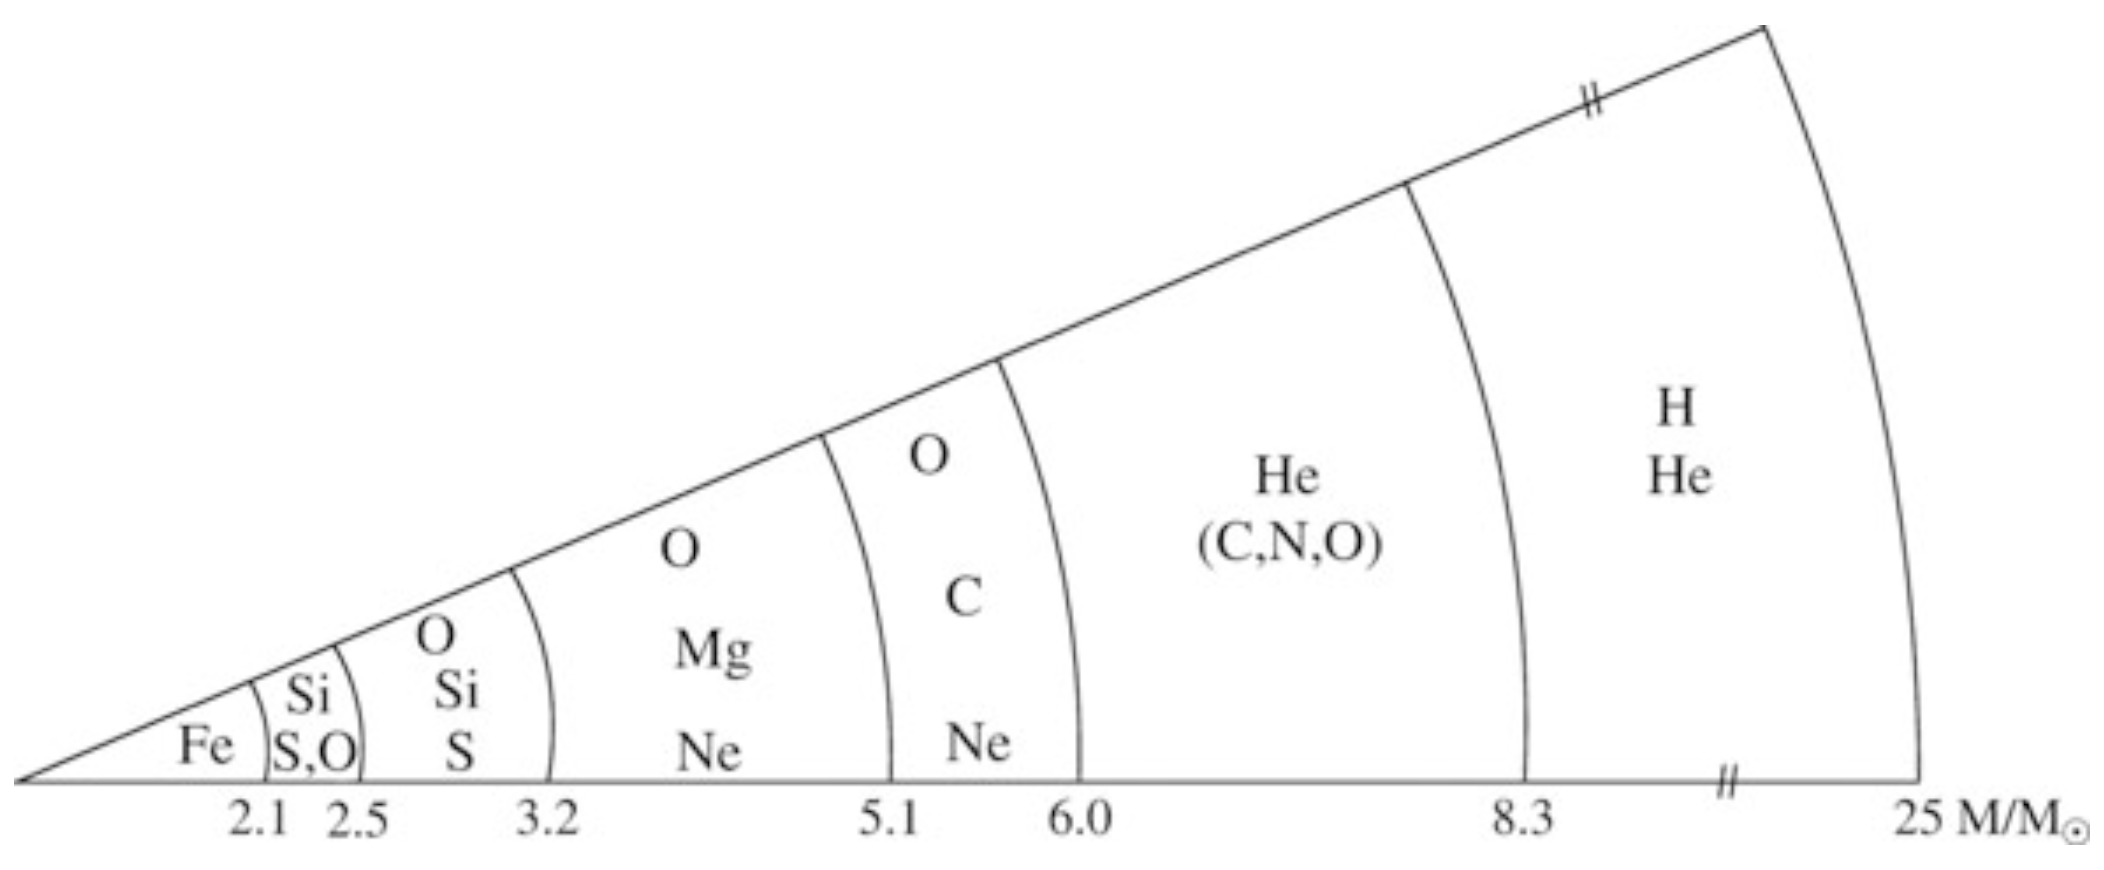
\includegraphics[width=12cm]{figures/ChemicalStructure.png}
    \caption{\footnotesize{Chemical shell structure of a massive star at the end of its life with the axis labeled by the mass within a given radius. The elements that have been formed in the various stages of the nuclear burning are ordered in a structure resembling that of an onion, with heavier elements being located closer to the center. This is the initial condition for a supernova explosion. Adapted from A. Uns\"{o}ld \& B. Baschek, The New Cosmos, Springer-Verlag. Figure taken from Schneider (2006).}}
    \label{fig:chemicalstructure}
\end{figure}

\begin{figure}[t]
    \centering
    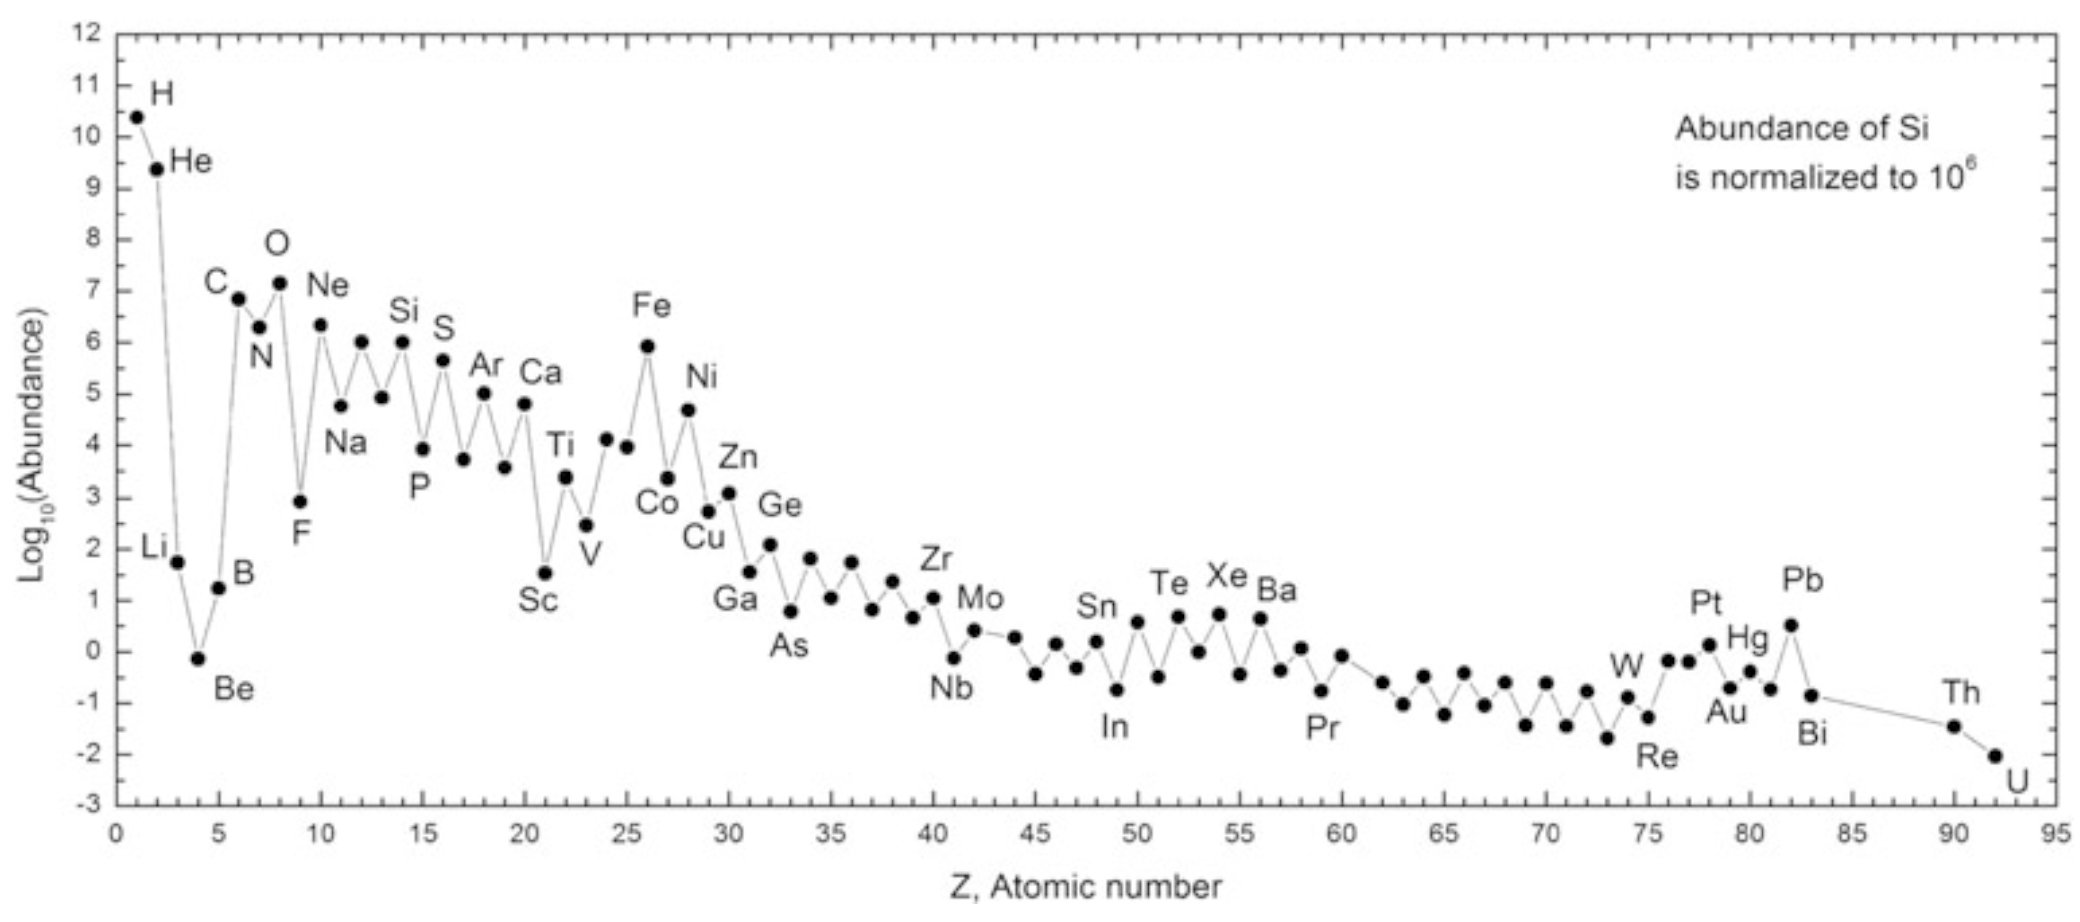
\includegraphics[width=12cm]{figures/ChemicalElements.png}
    \caption{\footnotesize{The relative abundance of chemical elements in the Solar System, normalized such that silicon attains the value $10^6$. As a general trend, the abundances decrease with increasing atomic number, except for the light elements lithium (Li), beryllium (Be), and boron (B), which are generated in stars, but also easily destroyed due to their low binding energy. Superposed on this decrease, the abundances show an oscillating behavior: nuclei with an even number of protons are more abundant than those with an odd atomic number -- this phenomenon is due to the production of alpha elements in core-collapse supernovae. Furthermore, iron (Fe), cobalt (Co) and nickel (Ni) stick out in their relatively high abundance, given their atomic number, which is due to their abundant production mainly in Type Ia SNe. Source: Wikipedia, numerical data from: Katharina Lodders. Figure taken from Schneider (2006).}}
    \label{fig:chemicalelements}
\end{figure}

{\noindent}\textbf{Type Ia supernovae}: SNe Ia are most likely the explosions of WDs. These compact stars which form the final evolutionary stages of less massive stars no longer maintain their internal pressure by nuclear fusion. Rather, they are stabilized by the degeneracy pressure of the electrons -- a quantum mechanical phenomenon related to the Fermi exclusion principle. Such a white dwarf can be stable only if its mass does not exceed a limiting mass, the \textbf{Chandrasekhar mass}; it has a value of $M_C\approx1.44\,{\rm M_\odot}$. For $M>M_C$, the degeneracy pressure can no longer balance the gravitational force. 

{\noindent}A WD can become unstable if its mass approaches the Chandrasekhar mass limit. There are two different scenarios with which this is possible: If the white dwarf is part of a close binary system, matter from the companion star may flow onto the WD; this is called the \textbf{`single-degenerate' model}. In this process, its mass will slowly increase and approach the limiting mass. At about $M\sim1.3\,{\rm M_\odot}$, carbon burning will ignite in its interior, transforming about half of the star into iron-group elements (i.e., iron, cobalt, and nickel). The resulting explosion of the star will enrich the ISM with $0.6\,{\rm M_\odot}$ of Fe, while the WD itself will be torn apart completely, leaving no remnant star. A second scenario (so-called \textbf{`double-degenerate'}) for the origin of SNe Ia is that of the merger of two WDs for which the sum of their masses exceeds the Chandrasekhar mass. Of course, these two scenarios are not mutually exclusive, and both routes may be realized in nature.

{\noindent}This interpretation of the different types of SNe explains why one finds core-collapse SNe only in galaxies in which star formation occurs. They are the final stages of massive (i.e., young) stars which have a lifetime of not more than $2\times10^7\,{\rm yr}$. By contrast, SNe Ia can occur in all types of galaxies, since their progenitors are members of an old stellar population.

{\noindent}Since the initial conditions are probably very homogeneous for the class of SNe Ia in the single-degenerate scenario (defined by the limiting mass prior to the trigger of the explosion), they are good candidates for standard candles: all SNe Ia have approximately the same luminosity. This is not entirely the case, but nevertheless SNe Ia play a very important role in the cosmological distance determination, and thus in the determination of cosmological parameters. On the other hand, in the double-degenerate scenario, the class of SNe Ia is not expected to be very homogeneous, as the mass prior to the explosion no longer attains a universal value. In fact, there are some SNe Ia which are clearly different from the majority of this class, by being far more luminous. It may be that such events are triggered by the merging of two white dwarfs, whereas the majority of the explosions is caused by the single-degenerate formation process.

Since Type Ia supernovae are supposed to be the result of explosion processes of white dwarfs which cross a critical mass threshold by accretion of additional matter, this threshold should be identical for all SNe Ia making it at least plausible that they all have the same luminosity. If this were the case, they would be ideal for standard candles: owing to their high luminosity, they can be detected and examined even at very large distances. 

\begin{figure}[t]
    \floatbox[{\capbeside\thisfloatsetup{capbesideposition={right,top},capbesidewidth=4cm}}]{figure}[\FBwidth]
    {\caption{\footnotesize{\\The Hubble diagram for relatively nearby SNe Ia. Plotted is the measured expansion velocity $cz$ as a function of the distance modulus for the individual supernovae. In the top panel, it is assumed that all sources have the same luminosity. In the bottom panel, the luminosities have been corrected by means of the so-called MLCS method in which the shape of the light curve and the colors of the SN are used to `standardize' the luminosity. By this the deviations from the Hubble law become dramatically smaller (the dispersion is reduced from $0.42$ to $0.15\,{\rm mag}$). Source: A.V. Filippenko \& A.G. Riess 2000, Evidence from Type Ia Supernovae for an Accelerating Universe, astro-ph/0008057, p. 5, Fig. 1. Figure taken from Schneider (2006).}}
    \label{fig:sneia}}
    {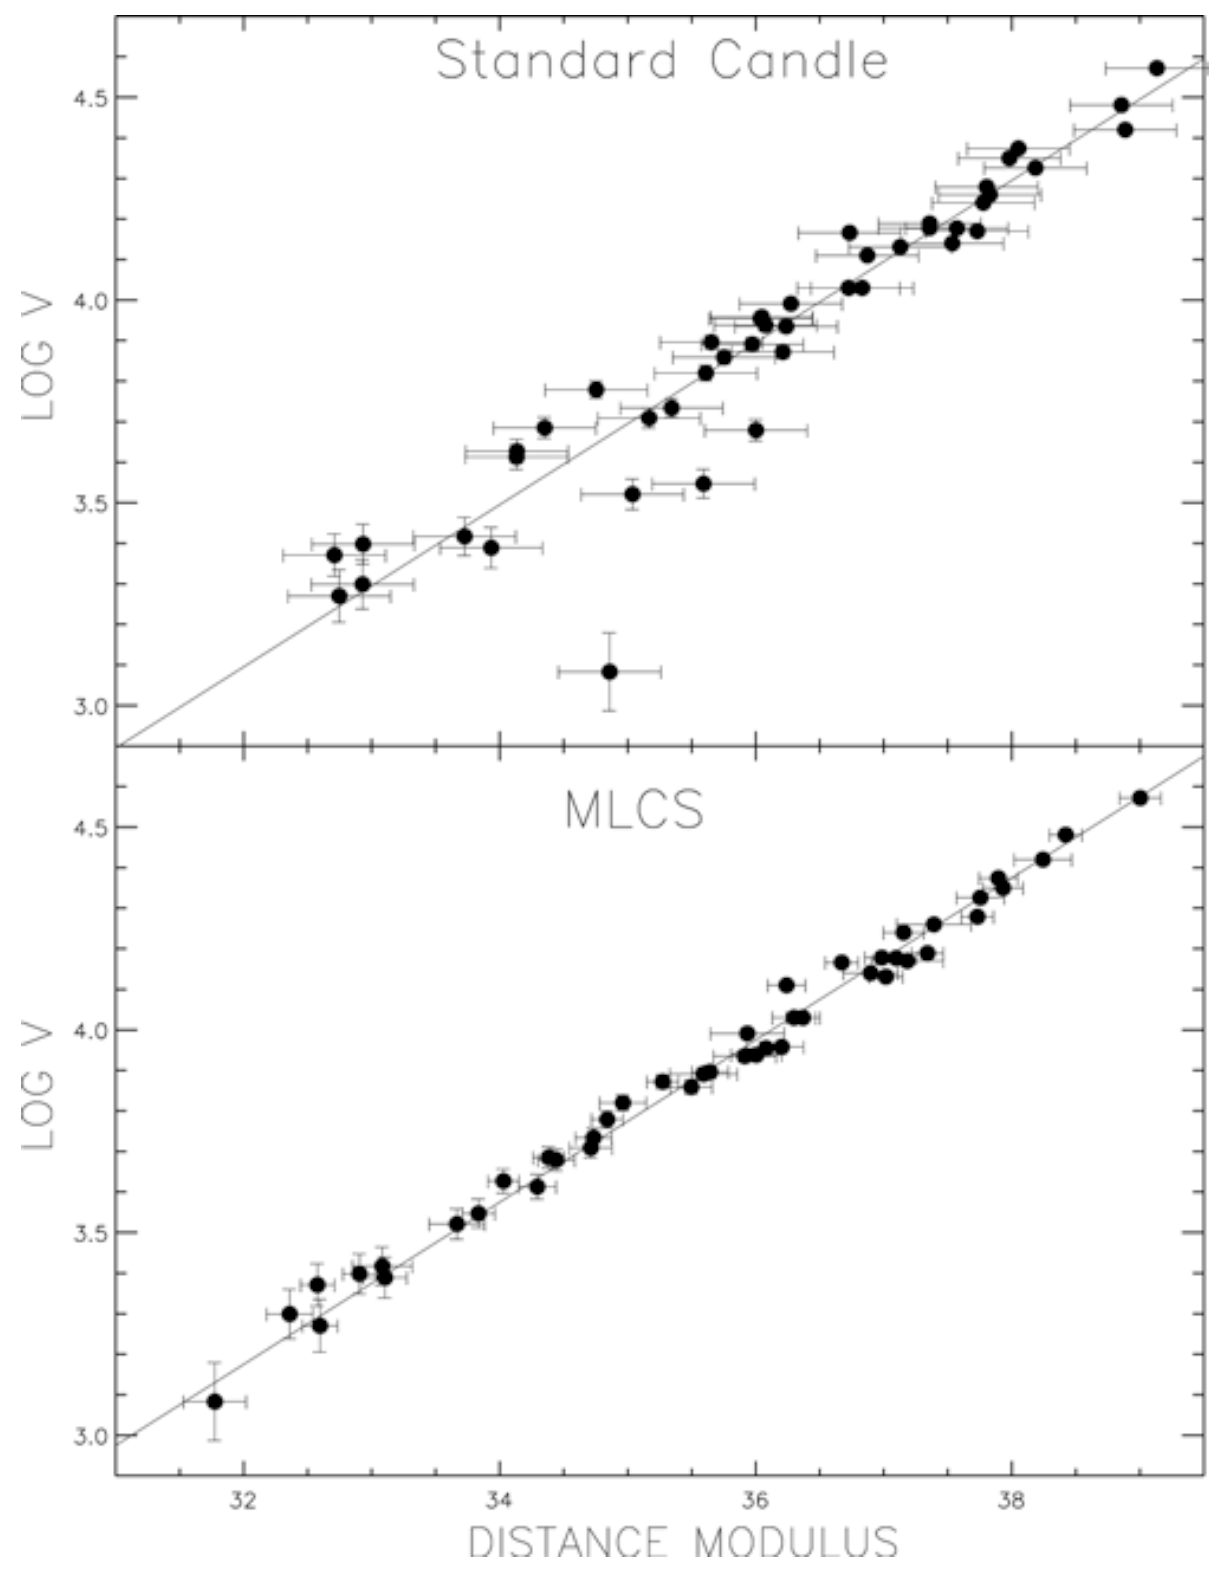
\includegraphics[width=8cm]{figures/SNeIa.png}}
\end{figure}

\begin{figure}[t]
    \centering
    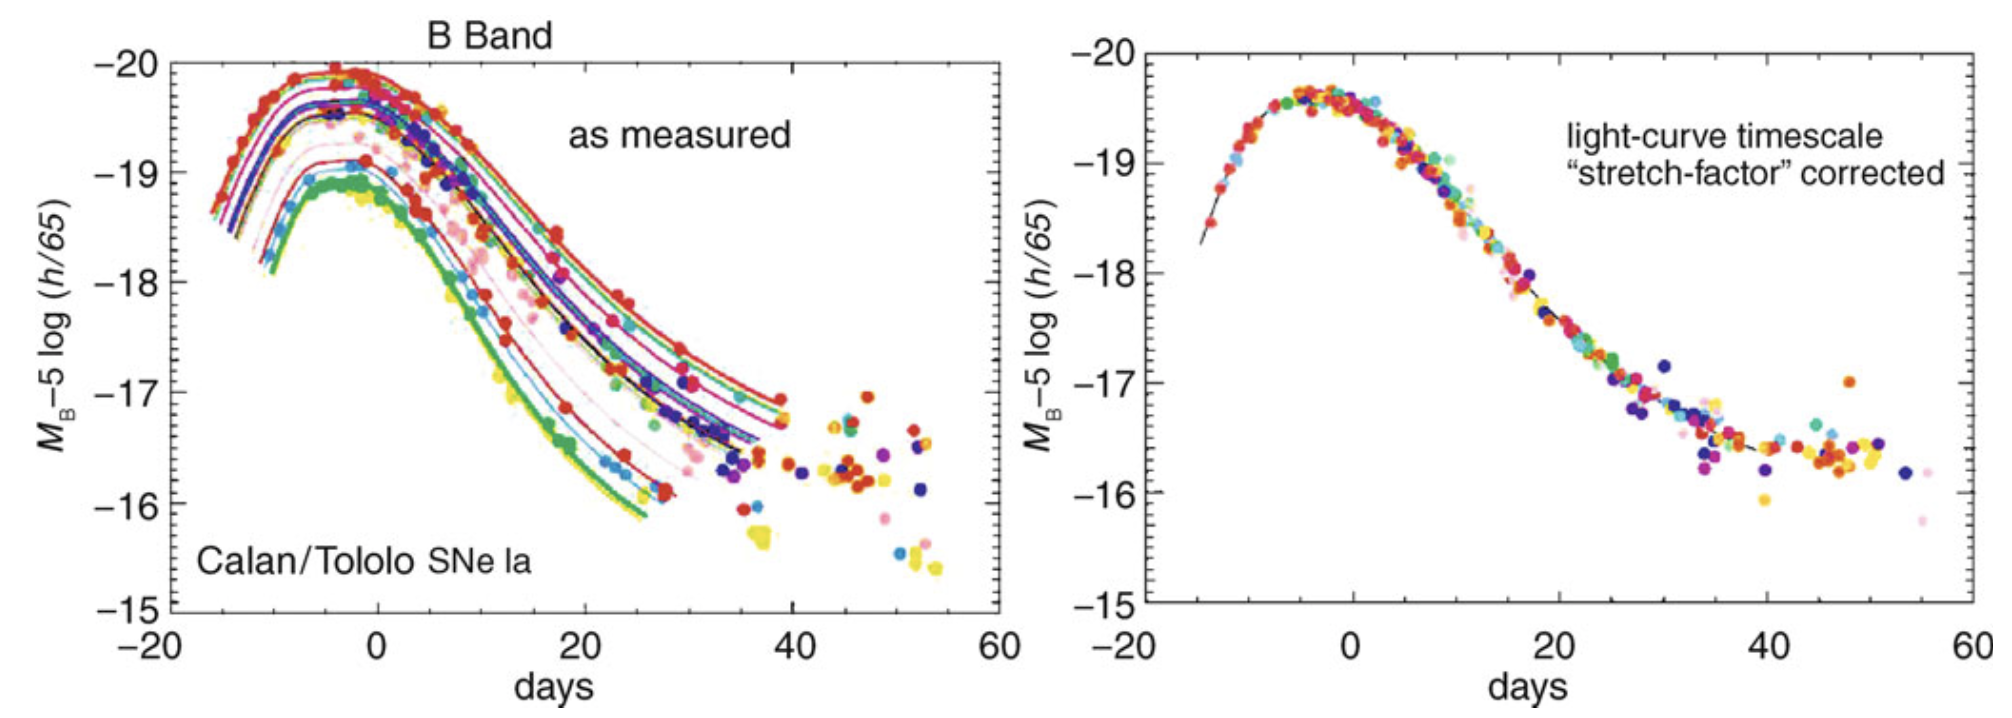
\includegraphics[width=16cm]{figures/SNeIa_corrected.png}
    \caption{\footnotesize{\textbf{Left panel:} B-band light curves of different SNe Ia. One sees that the shape of the light curves and the maximum luminosity of the SNe Ia differ substantially among the sample. A transformation was found empirically with a single parameter described by the width of the light curve. By means of this transformation, the different light curves can all be made congruent, as displayed in the \textbf{right panel}. Credit: M. Hamuy, S. Perlmutter, Supernova Cosmology Project. Figure taken from Schneider (2006).}}
    \label{fig:sneia_corrected}
\end{figure}

{\noindent}However, it turns out that SNe Ia are not really standard candles, since their maximum luminosity varies from object to object with a dispersion of about $0.4\,{\rm mag}$ in the blue band light. This is visible in the top panel of Figure \ref{fig:sneia}. If SNe Ia were standard candles, the data points would all be located on a straight line, as described by the Hubble law. Clearly, deviations from the Hubble law can be seen, which are significantly larger than the photometric measurement errors. It turns out that there is a strong correlation between the luminosity and the shape of the light curve of SNe Ia. Those of higher maximum luminosity show a slower decline in the light curve, as measured from its maximum. Furthermore, the observed flux is possibly affected by extinction in the host galaxy, in addition to the extinction in the MW. With the resulting reddening of the spectral distribution, this effect can be derived from the observed colors of the SN. The combined analysis of these effects provides a possibility for deducing an empirical correction to the maximum luminosity from the observed light curves in several filters, accounting both for the relation of the width of the curve to the observed luminosity and for the extinction. This correction was calibrated on a sample of SNe Ia for which the distance to the host galaxies is very accurately known. With this correction applied, the SNe Ia follow the Hubble law much more closely, as can be seen in the bottom panel of Figure \ref{fig:sneia}. A scatter of only $0.15\,{\rm mag}$ around the Hubble relation remains. Figure \ref{fig:sneia_corrected} demonstrates the effect of this correction on the light curves of several SNe Ia which initially appear to have very different maximum luminosities and widths. After correction they become nearly identical. The left panel of Figure \ref{fig:sneia_corrected} suggests that the light curves of SN Ia can basically be described by a one-parameter family of functions, and that this parameter can be deduced from the shape, in particular the width, of the light curves.

\subsubsection{Follow-up Questions}

\begin{itemize}
    \item When a star goes supernova, how much of the luminous energy generated at the rebound is available for heating the gas? As in, where does the heat come from?
    \item Are there cases where the rebound shock wave can't blow up the star? Why, and what happens then?
\end{itemize}

% --------------------------------------------------------------
%               8. 
% --------------------------------------------------------------

\newpage
\subsection{Question 8}

Describe the condition for a star's envelope to become convective. Why are low mass stars convective in their outer envelopes while high mass stars are convective in their inner cores?

\subsubsection{Short answer}

{\noindent}In general, convection will occur when

\begin{enumerate}
    \item the stellar opacity is large, implying that an unchievably steep temperature gradient would be necessary for radiative transport;
    \item a region exists where ionization is occurring, causing a large specific heat and a low adiabatic temperature gradient; and
    \item the temperature dependence of the nuclear energy generation rate is large, causing a steep radiative flux gradient and a large temperature gradient.
\end{enumerate}

{\noindent}In the atmosphere of many stars, the first two conditions can occur simultaneously, whereas the third condition would occur only deep in stellar interiors. In particular, the third condition can occur when the highly temperature-dependent CNO cycle or triple alpha processes are occurring.

{\noindent}The Sun is purely radiative below $r/{\rm D_\odot}=0.714$ and becomes convective above that point. Physically this occurs because the opacity in the outer portion of the Sun becomes large enough to inhibit the transport of energy by radiation Stars only slightly more massive than the Sun are convective in their centers because of the stronger temperature dependence of the CNO cycle as compared to the pp chain.

\subsubsection{Additional context}

{\noindent}Three different energy transport mechanisms operate in stellar interiors. \textbf{Radiation} allows the energy produced by nuclear reactions and gravitation to be carried to the surface via photons, the photons being absorbed and re-emitted in nearly random directions as they encounter matter. This suggests that the opacity of the material must play an important role, as one would expect. \textbf{Convection} can be a very efficient transport mechanism in many regions of a star, with hot, buoyant mass elements carrying excess energy outward while cool elements fall inward. Finally, \textbf{conduction} transports heat via collisions between particles. Although conduction can play an important role in some stellar environments, it is generally insignificant in most stars throughout the majority of their lifetimes. 

{\noindent}\textbf{Radiative transport of energy: basic estimates} Rough estimates show important features of the radiative transfer in stellar interiors and justify an enormous simplification of the formalism. Let us first estimate the mean free path $\ell_{\rm mfp}$ of a photon at an ``average'' point inside a star like the Sun:

\begin{align*}
    \ell_{\rm mfp} = \frac{1}{\kappa\rho} ~ [{\rm m}].
\end{align*}

{\noindent}where $\kappa$ is a mean absorption coefficient (i.e., a radiative cross section per unit mass averaged over frequency). Typical values for stellar material are of order $\kappa\approx1\,{\rm cm^2\,g^{-1}}$; for the ionized hydrogen in stellar interiors, a lower limit is certainly the value for electron scattering, $\kappa\approx0.4\,{\rm cm^2\,g^{-1}}$. Using this and the mean density of matter in the Sun, $\bar{\rho}_\odot=1.4\,{\rm g\,cm^{-3}}$, we obtain a mean free path of only

\begin{align*}
    \ell_{\rm mfp} = \frac{1}{\kappa\rho} = \frac{1}{1\,{\rm cm^2\,g^{-1}}\cdot0.4\,{\rm g\,cm^{-3}}} \approx2 ~ [{\rm cm}],
\end{align*}

{\noindent}i.e., stellar matter is very opaque.

{\noindent}The typical temperature gradient in the star can be roughly estimated by averaging between centre ($T_c\approx10^7\,{\rm K}$) and surface ($T_0\approx10^4\,{\rm K}$):

\begin{align*}
    \frac{\Delta T}{\Delta r} \approx \frac{T_c-T_0}{R_\odot} \approx 1.4\times10^{-4}\,[{\rm K\,cm^{-1}}].
\end{align*}

{\noindent}The radiation field at a given point is emitted from a small, nearly isothermal surrounding, the differences of temperature being only of order $\Delta T=\ell_{\rm mfp}({\rm d}T/{\rm d}r)\approx3\times10^{-4}\,{\rm K}$. Since the energy density of radiation is $u\sim T^4$, the relative anisotropy of the radiation at a point with $T=10^7\,{\rm K}$ is $\Delta T/T\sim10^{-10}$. The situation in stellar interiors must obviously be very close to TE, and the radiation very close to that of a blackbody. Nevertheless, the small remaining anisotropy can easily be the carrier of the stars' huge luminosity: this fraction of $10^{-10}$ of the flux emitted from ${\rm 1\,cm^2}$ of a blackbody of $T=10^7\,{\rm K}$ is still $10^3$ times larger than the flux at the solar surface ($6\times10^{10}\,{\rm erg\,cm^{-2}\,s^{-1}}$. Radiative transport of energy occurs via the non-vanishing net flux (i.e., via the surplus of the outwards-going radiation emitted from somewhat hotter material below over the inwards-going radiation emitted from less-hot material above).

{\noindent}\textbf{Diffusion of radiative energy:} The above estimates have shown that for radiative transport in stars, the mean free path $\ell_{\rm mfp}$ of the ``transporting particles'' (i.e., photons) is very small compared to the characteristic length $R$ (stellar radius) over which the transport extends: $\ell_{\rm mfp,\odot}/R_\odot\approx3\times10^{-11}$. In this case, the transport can be treated as a diffusion process, which yields an enormous simplification of the formalism. We derive the corresponding equation by analogy to those for particle diffusion.

{\noindent}The diffusive flux $j$ of particles (per unit area and time) between places of different particle density $n$ is given by

\begin{align*}
    \vec{j} = -D\nabla n,
\end{align*}

{\noindent}where $D$ is the coefficient of diffusion,

\begin{align*}
    D = \frac{1}{3}v\ell_{\rm mfp} ~ [{\rm s^{-1}}],
\end{align*}

{\noindent}determined by the average values of mean velocity $v$ and mean free path $\ell_{\rm mfp}$ of the particles.

{\noindent}In order to obtain the corresponding diffusive flux of radiative energy $\vec{F}$; we replace $n$ by the energy density of radiation $U$;

\begin{align*}
    u = aT^4 = \frac{4\sigma}{c}T^4 ~ [{\rm erg\,cm^{-3}}].
\end{align*}

{\noindent}Here, $a=7.57\times10^{-15}\,{\rm erg\,cm^{3}\,K^{-4}}$ is the \textbf{radiation density constant}. Owing to the spherical symmetry of the problem, $\vec{F}$ has only a radial component $F_r=\lvert\vec{F}\rvert=F$ and $\nabla U$ reduces to the derivative in the radial direction

\begin{align*}
    \frac{\partial u}{\partial r} = 4aT^3\frac{\partial T}{\partial r} ~ [{\rm erg\,cm^{-4}}].
\end{align*}

{\noindent}Using this result along with the equation for $\vec{j}$, this immediately gives us

\begin{align*}
    F = - \frac{4ac}{3} \frac{T^3}{\kappa\rho} \frac{\partial T}{\partial r} ~ [{\rm erg\,s^{-1}\,cm^{-2}}].
\end{align*}

{\noindent}Note that this can be interpreted formally as an \textbf{equation for heat conduction} by writing

\begin{align*}
    \vec{F} = -k_{\rm rad}\nabla T ~ [{\rm erg\,s^{-1}\,cm^{-2}}],
\end{align*}

{\noindent}where 

\begin{align*}
    k_{\rm rad} = \frac{4ac}{3} \frac{T^3}{\kappa\rho} ~ [{\rm erg\,cm^{-1}\,K^{-1}\,s^{-1}}]
\end{align*}

{\noindent}represents the \textbf{coefficient of conduction} for this radiative transport.

{\noindent}We solve $F$ for the gradient of the temperature and replace it by the usual local luminosity $L=4\pi r^2F$; then

\begin{align*}
    \frac{\partial T}{\partial r} = - \frac{3}{16\pi ac} \frac{\kappa\rho L}{r^2T^3} ~ [{\rm K\,cm^{-1}}]
\end{align*}

{\noindent}Of course, this neat and simple equation becomes invalid when one approaches the surface of the star. Because of the decreasing density, the mean free path of the photons will there become comparable with (and finally larger than) the remaining distance to the surface; hence the whole diffusion approximation breaks down, and one has to solve the far more complicated full set of transport equations for radiation in the stellar atmosphere (these equations indeed yield our simple diffusion approximation as the proper limiting case for large optical depths).

{\noindent}\textbf{The Rosseland mean for $\kappa_\nu$:} The above equations are independent of the frequency $\nu$; $F$ and $L$ are quantities integrated over all frequencies, so that the quantity   must represent a ``proper mean'' over $\nu$. We shall now prescribe a method for this averaging.

{\noindent}In general the absorption coefficient depends on the frequency $\nu$. Let us denote this by adding a subscript $\nu$ to all quantities that thus become frequency dependent: $\kappa_\nu$, $\ell_\nu$, $D_\nu$, $u_\nu$ etc.

{\noindent}For the diffusive energy flux $\vec{F}_\nu$ of radiation in the interval $[\nu,\nu+{\rm d}\nu]$, we write now

\begin{align*}
    \vec{F}_\nu &= -D_\nu \nabla u_\nu ~ [{\rm erg\,s^{-1}\,cm^{-2}}], \\
    D_\nu &= \frac{1}{3}c\ell_\nu = \frac{c}{3\kappa_\nu\rho} ~ [{\rm m^2\,s^{-1}}],
\end{align*}

{\noindent}while the energy density in the same interval is given by

\begin{align*}
    u_\nu = \frac{4\pi}{c}B(\nu,T) = \frac{8\pi h}{c^3} \frac{\nu^3}{e^{h\nu/k_BT}-1}  ~ [{\rm erg\,cm^{-3}}].
\end{align*}

{\noindent}$B(\nu,T)$ denotes here the \textbf{Planck function} for the intensity of blackbody radiation (differing from the usual formula for the energy density simply by the factor $4\pi/c$. From this equation for $u_\nu$, we have

\begin{align*}
    \nabla u_\nu = \frac{4\pi}{c} \frac{\partial B}{\partial T}\nabla T,
\end{align*}

{\noindent}which together with $D_\nu$ is inserted into  $F_\nu$, the latter then being integrated over all frequencies to obtain the total flux $F$: 

\begin{align*}
    \vec{F} = -\left[ \frac{4\pi}{3\rho} \int\limits_0^\infty \frac{1}{\kappa_\nu} \frac{\partial B}{\partial T} {\rm d}\nu \right] \nabla T ~ [{\rm m^2\,s^{-1}}].
\end{align*}

{\noindent}We have thus regained $\vec{F}=-k_{\rm rad}\nabla T$ with

\begin{align*}
    k_{\rm rad} = \frac{4\pi}{3\rho} \int\limits_0^\infty \frac{1}{\kappa_\nu} \frac{\partial B}{\partial T} {\rm d}\nu ~ [{\rm erg\,cm^{-1}\,K^{-1}\,s^{-1}}].
\end{align*}

{\noindent}Equating this expression for $k_{\rm rad}$ with that in the averaged form, we have immediately the proper formula for averaging the absorption coefficient:

\begin{align*}
    \frac{1}{\kappa} = \frac{\pi}{acT^3} \int\limits_0^\infty \frac{\partial B}{\partial T} {\rm d}\nu ~ [{\rm cm^2\,g^{-1}}].
\end{align*}

{\noindent}This is the so-called \textbf{Rosseland mean}. Since

\begin{align*}
    \int\limits_0^\infty \frac{\partial B}{\partial T}{\rm d}\nu = \frac{acT^3}{\pi},
\end{align*}

{\noindent}the Rosseland mean is formally the harmonic mean of    with the weighting function $\partial B/\partial T$, and it can simply be calculated, once the function $\kappa_\nu$ is known from atomic physics.

{\noindent}In order to see the physical interpretation of the Rosseland mean, we rewrite $\vec{F}_\nu=-D_\nu\nabla u_\nu$ as

\begin{align*}
    \vec{F}_\nu = -\left(\frac{1}{\kappa_\nu}\frac{\partial B(\nu,T)}{\partial T}\right)\frac{4\pi}{3\rho}\nabla T ~ [{\rm m^2\,s^{-1}}].
\end{align*}

{\noindent}This shows that, for a given point in the star ($\rho$ and $\nabla T$ given), the integrand in $1/\kappa$ is at all frequencies proportional to the net flux $\vec{F}_\nu$ of energy. The Rosseland mean therefore favours the frequency ranges of maximum energy flux. One could say that an average \textit{transparency} is evaluated rather than an \textit{opacity} -- which is plausible, since it is to be used in an equation describing the transfer of energy rather than its blocking.

{\noindent}One can also easily evaluate the frequency where the weighting function $\partial B/\partial T$ has its maximum. One finds that, for given a temperature, $\partial B/\partial T\sim x^4e^x(e^x-1)^{-2}$ with $x=h\nu/k_BT$. Differentiation with respect to $x$ shows that the maximum of $\partial B/\partial T$ is close to $x=4$.

{\noindent}The way we have defined the Rosseland mean $\kappa$, which is a kind of weighted harmonic mean value, has the uncomfortable consequence that the opacity $\kappa$ of a mixture of two gases having the opacities $\kappa_1,\kappa_2$ is not the sum of the opacities: $\kappa\neq\kappa_1\kappa_2$. Therefore, in order to find $\kappa$ for a mixture containing the weight fractions $X$ of hydrogen and $Y$ of helium, the mean opacities of the two single gases are of no use. Rather one has to add the frequency-dependent opacities $\kappa_\nu=X_{\kappa_\nu,{\rm H}}+Y_{\kappa_\nu,{\rm He}}$ before calculating the Rosseland mean. For any new abundance ratio $X/Y$ the averaging over the frequency has to be carried out separately.

{\noindent}In the above we have characterized the energy flux due to the diffusion of photons by $F_\nu$. Since in the following we shall encounter other mechanisms for energy transport, from now on we shall specify this radiative flux by the vector $\vec{F}_{\rm rad}$. Correspondingly we shall use $\kappa_{\rm rad}$ instead of  $\kappa$, etc.

{\noindent}\textbf{Conductive transport of energy:} In heat conduction, energy transfer occurs via collisions during the random thermal motion of the particles (electrons and nuclei in completely ionized matter, otherwise atoms or molecules). A basic estimate shows that in ``ordinary'' stellar matter (i.e., in a non-degenerate gas), conduction has no chance of taking over an appreciable part of the total energy transport. Although the collisional cross sections of these charged particles are rather small at the high temperatures in stellar interiors $(10^{-18}-10^{-20}\,cm^2$ per particle), the large density ($\rho=1.4\,{\rm g\,cm^{-3}}$ in the Sun) results in mean free paths several orders of magnitude less than those for photons; and the velocity of the particles is only a few per cent of $c$. Therefore the coefficient of diffusion is much smaller than that for photons.

{\noindent}The situation becomes quite different, however, for the cores of evolved stars where the electron gas is highly degenerate. The density can be as large as $10^6\,{\rm g\,cm^{-3}}$. But degeneracy makes the electrons much faster, since they are pushed up close to the Fermi energy; and degeneracy increases the mean free path considerably, since the quantum cells of phase space are filled up such that collisions in which the momentum is changed become rather improbable. Then the coefficient of diffusion (which is proportional to the product of mean free path and particle velocity) is large, and heat conduction can become so efficient that it short-circuits the radiative transfer.

{\noindent}The energy flux $\vec{F}_{\rm cd}$ due to heat conduction may be written as

\begin{align*}
    \vec{F}_{\rm cd} = -k_{\rm cd}\nabla T ~ [{\rm m^2\,s^{-1}}].
\end{align*}

{\noindent}The sum of the conductive flux $\vec{F}_{\rm cd}$ and the radiative flux $\vec{F}_{\rm rad}$ is

\begin{align*}
    \vec{F} = \vec{F}_{\rm rad}+\vec{F}_{\rm cd} = -(k_{\rm rad}+k_{\rm cd})\nabla T ~ [{\rm m^2\,s^{-1}}],
\end{align*}

{\noindent}On the other hand, we can just as well write the conductive coefficient $k_{\rm cd}$ formally in analogy to $k_{\rm rad}$ as

\begin{align*}
    k_{\rm cd} = \frac{4ac}{3}\frac{T^3}{\kappa_{\rm cd}\rho} ~ [{\rm cm^2\,g^{-1}}],
\end{align*}

{\noindent}hence defining the \textbf{conductive opacity} $\kappa_{\rm cd}$. Then the flux becomes

\begin{align*}
    \vec{F} = -\frac{4ac}{3}\frac{T^3}{\rho} \left(\frac{1}{\kappa_{\rm rad}}+\frac{1}{\kappa_{\rm cd}}\right) \nabla T,
\end{align*}

{\noindent}which shows that we arrive formally at the same type of equation as in the pure radiative case if we replace $1/\kappa$ by $1/\kappa_{\rm rad}+1/\kappa_{\rm cd}$. Again the result is plausible, since the mechanism of transport that provides the largest flux will dominate the sum (i.e., the mechanism for which the stellar matter has the highest ``transparency'').

{\noindent}The basic equation for energy transport which, if we define properly, holds for radiative and conductive energy transport, can be rewritten in a convenient form. Starting with

\begin{align*}
    \frac{\partial T}{\partial r} = - \frac{3}{16\pi ac} \frac{\kappa\rho L}{r^2T^3} ~ [{\rm K\,cm^{-1}}],
\end{align*}

{\noindent}we can transform to the independent variable mass $m$ using the fact that $\partial r/\partial m = (4\pi r^2\rho)^{-1}$:

\begin{align*}
    \frac{\partial T}{\partial m} = - \frac{3}{64\pi^2 ac} \frac{\kappa L}{r^4T^3} ~ [{\rm K\,g^{-1}}].
\end{align*}

{\noindent}Assuming hydrostatic equilibrium, we can divide this by $\partial P/\partial r = -(Gm\rho)/r^2$ and obtain

\begin{align*}
    \frac{(\partial T/\partial m)}{(\partial P/\partial m)} = \frac{3}{16\pi acG}\frac{\kappa L}{mT^3} ~ [{\rm K\,P\,g^{-2}}].
\end{align*}

{\noindent}We call the ratio of the derivatives on the left $({\rm d}T/{\rm d}P)_{\rm rad}$, and we mean by this the variation of $T$ in the star with depth, where the depth is expressed by the pressure, which increases monotonically inwards. In this sense, in a star which is in hydrostatic equilibrium and transports the energy by radiation (and conduction), $({\rm d}T/{\rm d}P)_{\rm rad}$ is a gradient describing the temperature variation with depth. If we use the customary abbreviation

\begin{align*}
    \nabla_{\rm rad} \equiv \left(\frac{{\rm d}\ln T}{{\rm d}\ln P}\right)_{\rm rad} ~ [{\rm K\,P^{-1}}],
\end{align*}

{\noindent}which can be written in the form

\begin{align*}
    \nabla_{\rm rad} = \frac{3}{16\pi acG}\frac{\kappa LP}{mT^4} ~ [{\rm K\,P^{-1}}],
\end{align*}

{\noindent}in which conduction effects are now included. $\nabla_{\rm rad}$ means a spatial derivative (connecting $P$ and $T$ in two neighbouring mass shells), while $\nabla_{\rm ad}$ describes the thermal variation of one and the same mass element during its adiabatic compression. Only in special cases $({\rm d}\ln T/{\rm d}\ln P)$ and $\nabla_{\rm ad}$ will have the same value, and we then speak of an \textbf{adiabatic stratification}.

{\noindent}\textbf{Transport of energy by convection:} Convective transport of energy means an exchange of energy between hotter and cooler layers in a dynamically unstable region through the exchange of macroscopic mass elements (``blobs'', ``bubbles'', ``convective elements''), the hotter of which move upwards while the cooler ones descend. The moving mass elements will finally dissolve in their new surroundings and thereby deliver their excess (or deficiency) of heat. Owing to the high density in stellar interiors, convective transport can be very efficient. However, this energy transfer can operate only if it finds a sufficient driving mechanism in the form of the buoyancy forces.

{\noindent}A thorough theoretical treatment of convective motions and transport of energy is extremely difficult. It is the prototype of the many astrophysical problems in which the bottleneck preventing decisive progress is the difficulty involved in solving the well-known hydrodynamic equations. For simplifying assumptions, solutions are available that may even give reasonable approximations for certain convective flows in the laboratory. Unfortunately, convection in stars proceeds under rather malicious conditions: turbulent motion transports enormous fluxes of energy in a very compressible gas, which is stratified in density, pressure, temperature, and gravity over many powers of ten. Nevertheless, large efforts have been made over many years to solve this notorious problem, and they have partly arrived at promising results. None of the so-called Reynolds stress models, however, have reached a stage where it could provide a procedure easy enough to be handled in everyday stellar-structure calculations, and at the same time would describe the full properties of convection accurately enough. On the other hand, full two- and three-dimensional hydrodynamical simulations have also made large progress, thanks to the impressive advances in supercomputer technology and efficient numerical algorithms. They give valuable hints to the true nature of convection and often serve as numerical experiments to test the dynamical methods. Nevertheless, these numerical simulations are still limited in their size and thus can follow convection in most cases only for a limit time and only for thin convection zones. But even if these restrictions can be foreseen to get relaxed with time, such full hydrodynamical simulations will never be used in full stellar evolution models, as they would unnecessarily follow the star's evolution on a dynamical timescale, which is so much shorter than the dominant nuclear one. Therefore, we limit ourselves exclusively to the description of the old so-called \textbf{mixing-length} theory. The reason for this is not that we believe it to be sufficient, but it does provide at least a simple method for treating convection locally, at any given point of a star. Moreover, empirical tests of the resulting stellar models show a surprisingly good agreement with observations. And, finally, even this poor approximation shows without any doubt that in the very deep interior of a star, a detailed theory is normally not necessary.

{\noindent}Note that in the following we are dealing only with convection in stars that are in hydrostatic equilibrium. We furthermore assume that the convection is time independent, which means that it is fully adjusted to the present state of the star. Otherwise, a convection theory for rapidly changing regions (time-dependent convection) has to be developed.

{\noindent}The gradient $\nabla_{\rm rad}$ is what would be maintained in a star if the whole luminosity $L$ had to be transported outwards by radiation only. If convection contributes to the energy transport, the actual gradient $\nabla$ will be different (namely smaller). In the following, we will estimate $\nabla$ in the case of convection.

{\noindent}\textbf{The basic picture:} The mixing-length theory goes back to Ludwig Prandtl, who in 1925 modelled a simple picture of convection in complete analogy to molecular heat transfer: the transporting ``particles'' are macroscopic mass elements (``blobs'') instead of molecules; their mean free path is the \textbf{mixing length} after which the blobs dissolve in their new surroundings. Prandtl's theory was adapted for stars afterwards.

The radiation pressure gradient is given by 

\begin{align*}
    \frac{{\rm d}P_{\rm rad}}{{\rm d}r} = -\frac{\kappa\rho}{c}F_{\rm rad} ~ [{\rm P\,m}],
\end{align*}

{\noindent}where $F_{\rm rad}$ is the outward radiative flux. The radiation pressure may also be expressed as

\begin{align*}
    \frac{{\rm d}P_{\rm rad}}{{\rm d}r} = \frac{4}{3} aT^3 \frac{{\rm d}T}{{\rm d}r} ~ [{\rm P\,m}].
\end{align*}

{\noindent}Equating the two, we have

\begin{align*}
    \frac{{\rm d}T}{{\rm d}r} = -\frac{3}{4ac}\frac{\kappa\rho}{T^3}F_{\rm rad} ~ [{\rm K\,m^{-1}}].
\end{align*}

{\noindent}If we use the expression for the radiative flux written in terms of the local radiative luminosity of the star at radius $r$, 

\begin{align*}
    F_{\rm rad} = \frac{L_r}{4\pi r^2} ~ [{\rm erg\,s^{-1}\,cm^{-2}}],
\end{align*}

{\noindent}the temperature gradient for radiative transport becomes

\begin{align*}
    \frac{{\rm d}T}{{\rm d}r} = -\frac{3}{4ac}\frac{\kappa\rho}{T^3}\frac{L_r}{4\pi r^2} ~ [{\rm K\,m^{-1}}].
\end{align*}

{\noindent}As either the flux or the opacity increases, the temperature gradient must become steeper (i.e., more negative) if radiation transport is to carry all of the required luminosity outward. The same situation holds as the density increases or the temperature increases.

{\noindent}We now consider a situation where a hot convective bubble of gas rises and expands \textbf{adiabatically}, meaning that the bubble does not exchange heat with its surroundings. After it has travelled some distance, it finally \textbf{thermalizes}, giving up any excess heat as it loses its identity and dissolves into the surrounding gas. Differentiating the \textbf{ideal gas law}

\begin{align*}
    P = \frac{\rho k_BT}{\mu m_{\rm H}} ~ [{\rm P}]
\end{align*}

{\noindent}yields an expression involving the bubble's \textbf{temperature gradient}

\begin{align*}
    \frac{{\rm d}P}{{\rm d}r} = -\frac{P}{\mu}\frac{{\rm d}\mu}{{\rm d}r} + \frac{P}{\rho}\frac{{\rm d}\rho}{{\rm d}r} + \frac{P}{T}\frac{{\rm d}T}{{\rm d}r}.
\end{align*}

{\noindent}Using the adiabatic relationship between pressure and density

\begin{align*}
    PV^\gamma = K ~ [{\rm P\,m^3}]
\end{align*}

{\noindent}and recalling that $V\equiv1/\rho$ is the \textbf{specific volume}, we have that

\begin{align*}
    P = K\rho^\gamma ~ [{\rm P}].
\end{align*}

{\noindent}Differentiating and re-writing, we obtain

\begin{align*}
    \frac{{\rm d}P}{{\rm d}r} = \gamma \frac{P}{\rho}\frac{{\rm d}\rho}{{\rm d}r} ~ [{\rm P\,m^{-1}}].
\end{align*}

{\noindent}If we assume for simplicity that the mean molecular weight $\mu$ is constant, we can combing equations for ${\rm d}P/{\rm d}r$ to give the \textbf{adiabatic temperature gradient}

\begin{align*}
    \left(\frac{{\rm d}T}{{\rm d}r}\right)_{\rm ad} = \left(1-\frac{1}{\gamma}\right) \frac{T}{P}\frac{{\rm d}P}{{\rm d}r} ~ [{\rm K\,m^{-1}}].
\end{align*}

{\noindent}Using the equation of \textbf{hydrostatic equilibrium}

\begin{align*}
    \frac{{\rm d}P}{{\rm d}r} = -\frac{GM_r\rho}{r^2} = -\rho g ~ [{\rm P\,m^{-1}}], ~~~ g \equiv \frac{GM_r}{r^2} ~ [{\rm m\,s^{-2}}]
\end{align*}

{\noindent}and the ideal gas law, we finally obtain

\begin{align*}
    \left(\frac{{\rm d}T}{{\rm d}r}\right)_{\rm ad} = \left(1-\frac{1}{\gamma}\right) \frac{\mu m_{\rm H}}{k}\frac{GM_r}{r^2} ~ [{\rm K\,m^{-1}}].
\end{align*}

{\noindent}If the star's actual temperature gradient is \textit{steeper} than the adiabatic temperature gradient,

\begin{align*}
    \left\lvert\frac{{\rm d}T}{{\rm d}r}\right\rvert_{\rm act} > \left\lvert\frac{{\rm d}T}{{\rm d}r}\right\rvert_{\rm ad} ~ [{\rm K\,m^{-1}}],
\end{align*}

{\noindent}the temperature gradient is said to be \textbf{super-adiabatic} (recall that ${\rm d}T/{\rm d}r<0$). In the deep interior of a star, if the actual temperature gradient is just \textit{slightly} larger than the adiabatic temperature gradient, this may be sufficient to carry nearly all of the luminosity by convection. Consequently, it is often the case that either radiation or convection dominates the energy transport in the deep interior of stars, while the other energy transport mechanism contributes very little to the total energy outflow. The particular mechanism in operation is determined by the temperature gradient. However, near the surface of the star, the situation is much more complicated: both radiation and convection can carry significant amounts of energy simultaneously.

{\noindent}This condition for convection can be used to find another useful relation. Since ${\rm d}T/{\rm d}r<0$and $1/\gamma-1<0$ (recall that $\gamma>1$),

\begin{align*}
    \frac{T}{P}\left(\frac{{\rm d}T}{{\rm d}r}\right)^{-1} \frac{{\rm d}P}{{\rm d}r} < -\frac{1}{\gamma^{-1}-1} ~ [{\rm dimensionless}],
\end{align*}

{\noindent}which may be simplified to give

\begin{align*}
    \frac{T}{P}\frac{{\rm d}P}{{\rm d}T} < \frac{\gamma}{\gamma-1} ~ [{\rm dimensionless}],
\end{align*}

{\noindent}or, for convection to occur,

\begin{align*}
    \frac{{\rm d}\ln P}{{\rm d}\ln T} < \frac{\gamma}{\gamma-1} ~ [{\rm P\,K^{-1}}].
\end{align*}

{\noindent}For an ideal monatomic gas, $\gamma=5/3$ and convection will occur in some region of a star when ${\rm d}\ln P/{\rm d}\ln T<2.5$. In that case, the temperature gradient (${\rm d}T/{\rm d}r$) is given approximately by 

\begin{align*}
    \left(\frac{{\rm d}T}{{\rm d}r}\right)_{\rm ad} = -\left(1-\frac{1}{\gamma}\right) \frac{\mu m_{\rm H}}{k} \frac{GM_r}{r^2} ~ [{\rm K\,m^{-1}}].
\end{align*}

{\noindent}By comparing this with the temperature gradient for radiative transport

\begin{align*}
    \frac{{\rm d}T}{{\rm d}r} = - \frac{3}{4ac} \frac{\bar{\kappa}\rho}{T^3} \frac{L_r}{4\pi r^2} ~ [{\rm K\,m^{-1}}]
\end{align*}

{\noindent}together with the condition for convection written in terms of the temperature gradient, 

\begin{align*}
    \left\lvert\frac{{\rm d}T}{{\rm d}r}\right\rvert_{\rm act} > \left\lvert\frac{{\rm d}T}{{\rm d}r}\right\rvert_{\rm ad} ~ [{\rm K\,m^{-1}}],
\end{align*}

{\noindent}it is possible to develop some understanding of which conditions are likely to lead to convection over radiation. In general, convection will occur when

\begin{enumerate}
    \item the stellar opacity is large, implying that an unchievably steep temperature gradient would be necessary for radiative transport;
    \item a region exists where ionization is occurring, causing a large specific heat and a low adiabatic temperature gradient; and
    \item the temperature dependence of the nuclear energy generation rate is large, causing a steep radiative flux gradient and a large temperature gradient.
\end{enumerate}

{\noindent}In the atmosphere of many stars, the first two conditions can occur simultaneously, whereas the third condition would occur only deep in stellar interiors. In particular, the third condition can occur when the highly temperature-dependent CNO cycle or triple alpha processes are occurring.

{\noindent}\textbf{Convective regions}: Knowledge of the extension of convective regions is very important in view of their influence on the ensuing chemical evolution. A rough overview can be obtained from Fig. 22.7, where $m/M$ and $\log M/{\rm M_\odot}$ are ordinate and abscissa. For any given stellar mass $M$ along a line parallel to the ordinate it is indicated what conditions we would encounter when drilling a radial borehole from the surface to the centre. In particular, one can see whether the corresponding mass elements are convective or radiative. Aside from the stars of smallest mass ($M<0.25\,{\rm M_\odot}$), we can roughly distinguish between two types of models:

\begin{align*}
    {\rm radiative\,core+convective\,envelope\,(lower\,MS)} \\
    {\rm convective\,core+radiative\,envelope\,(upper\,MS)}.
\end{align*}

{\noindent}The transition from one type to the other occurs near $M=1\,{\rm M)\odot}$.

{\noindent}The distinction between convective and radiative regions is made here by using the \textbf{Schwarzschild criterion}, which predicts convection if the radiative gradient of temperature $\nabla_{\rm rad}$ exceeds the adiabatic gradient $\nabla_{\rm ad}$. The variation of these gradients (together with that of the actual gradient $\nabla$) throughout the star is plotted in Fig. 22.8 for $M=1\,{\rm M}$ and $10\,{\rm M}$. For the abscissa, $\log T$ is chosen, since this conveniently stretches the scale in the complicated outer layers.

{\noindent}Let us start with the simpler situation concerning the convective core. When comparing Figure \ref{fig:delT}a, b, we see that the convective core in the more massive models is caused by a steep increase of $\nabla_{\rm rad}$ towards the centre. The reason for this is that the dominating CNO cycle, with its extreme temperature sensitivity, concentrates the energy production very much towards the centre (cf. the curve l=L D 0:5 in Fig. 22.7, and Fig. 22.4e). Therefore we find in these stars very high fluxes of energy ($L=4\pi r^2$) at small $r$, which produce large values of $\nabla_{\rm rad}$. Figure \ref{fig:convectiveregions} shows a remarkable increase in the extent of the convective core for increasing $M$. The core covers as much as $65\%$ of the stellar mass in a star of $50\,{\rm M}$, an increase caused by the increasing radiation pressure which depresses the value of $\nabla_{\rm ad}$ well below its standard value of $0.4$ for an ideal monatomic gas. In the centre of the $50\,{\rm M}$ model, roughly $1/3$ of $P$ is radiation pressure, and $\nabla_{\rm ad}\approx0.27$. From Figure \ref{fig:delT}b it is clear that a depression of $\nabla_{\rm ad}$ in the central region will shift the intersection with $\nabla_{\rm rad}$ (i.e., the border of the convective core) outwards to smaller $T$. When we increase $M$ to much larger values still, the top of the convective core will finally approach the surface such that we should obtain fully convective stars. We then approach models of the so-called \textbf{supermassive stars}.

{\noindent}In less massive stars, the pp chain with its smaller temperature sensitivity dominates. This distributes the energy production over a much larger area, so that the flux ($L/4\pi r^2$) and $\nabla_{\rm rad}$ are much smaller in the central region, which thus remains radiative.

\begin{figure}[t]
    \floatbox[{\capbeside\thisfloatsetup{capbesideposition={right,top},capbesidewidth=4cm}}]{figure}[\FBwidth]
    {\caption{\footnotesize{\\The mass values $m$ from centre to surface are plotted against the stellar mass $M$ for the same ZAMS models as in Fig. 22.1. ``Cloudy'' areas indicate the extension of convective zones inside the models. Two solid lines give the $m$ values at which $r$ is $1/4$ and $1/2$ the total radius $R$: The dashed and dotted lines show the mass elements inside which 50\% and 90\% of the total luminosity $L$ are produced. Figure taken from Kippenhahn, Weigert \& Weiss (2012).}}
    \label{fig:convectiveregions}}
    {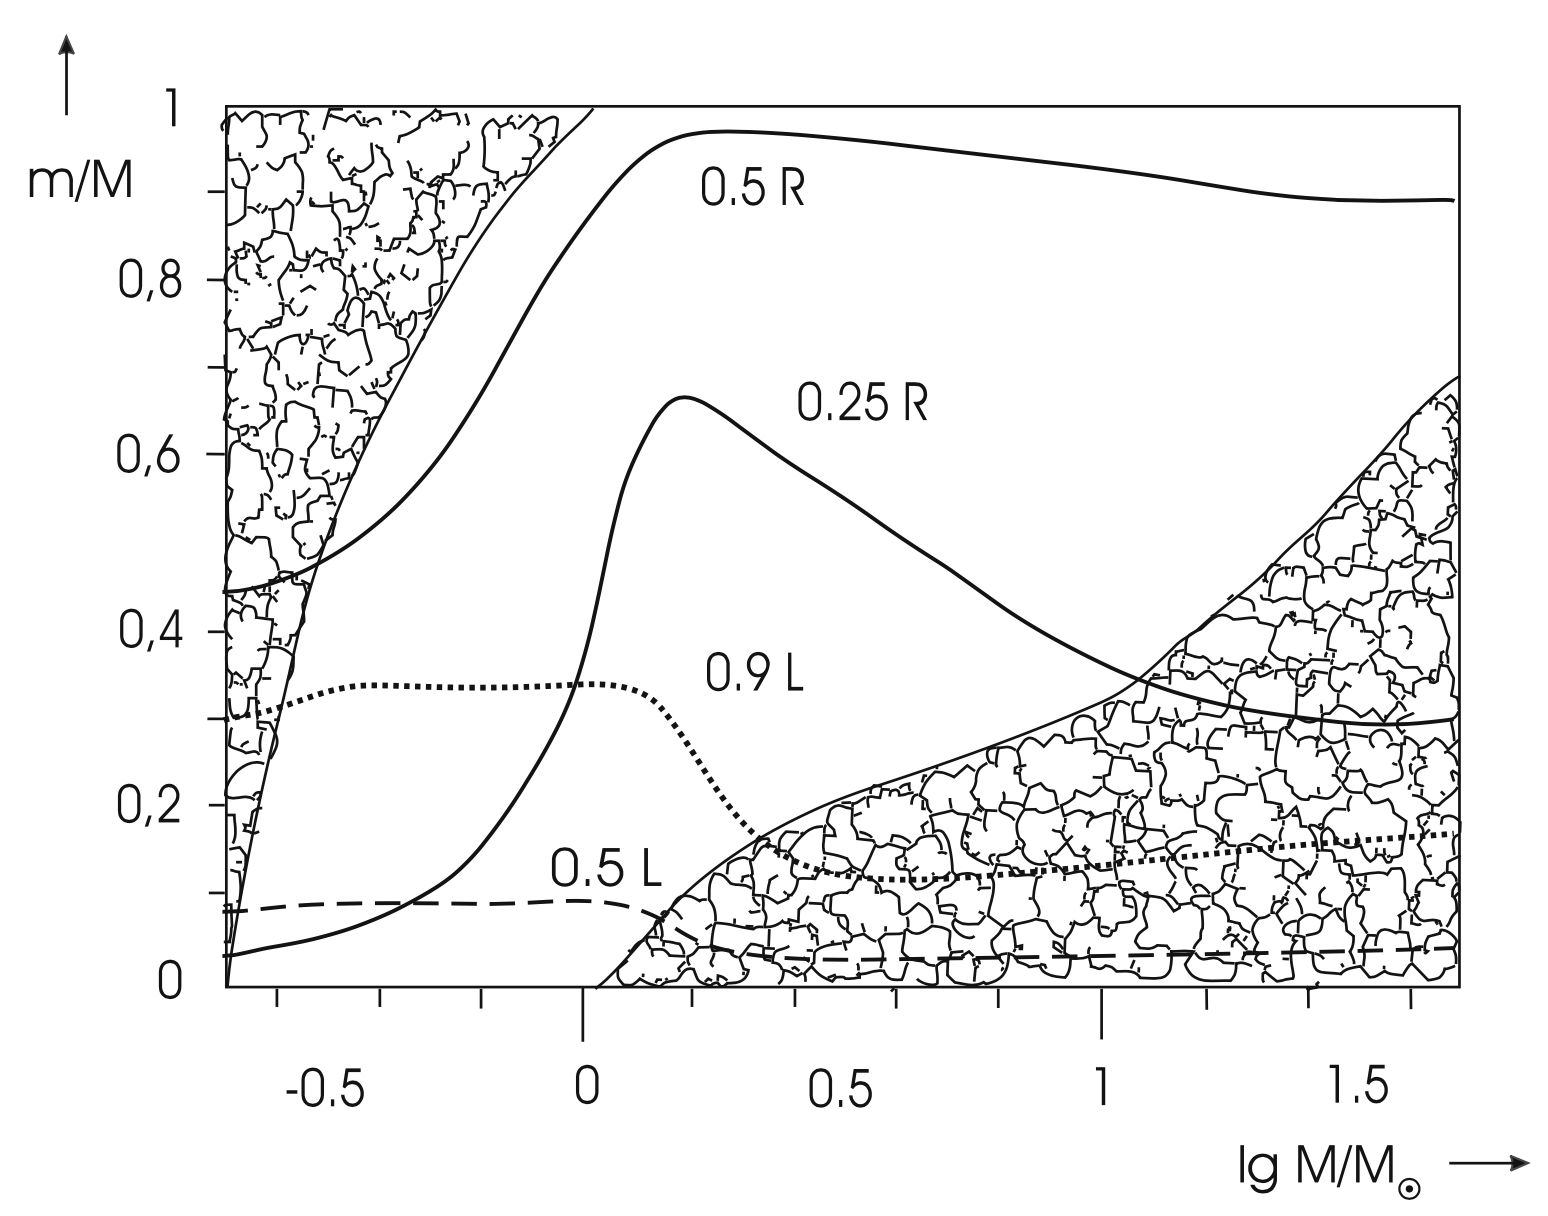
\includegraphics[width=8cm]{figures/ConvectiveRegions.png}}
\end{figure}

\begin{figure}[t]
    \centering
    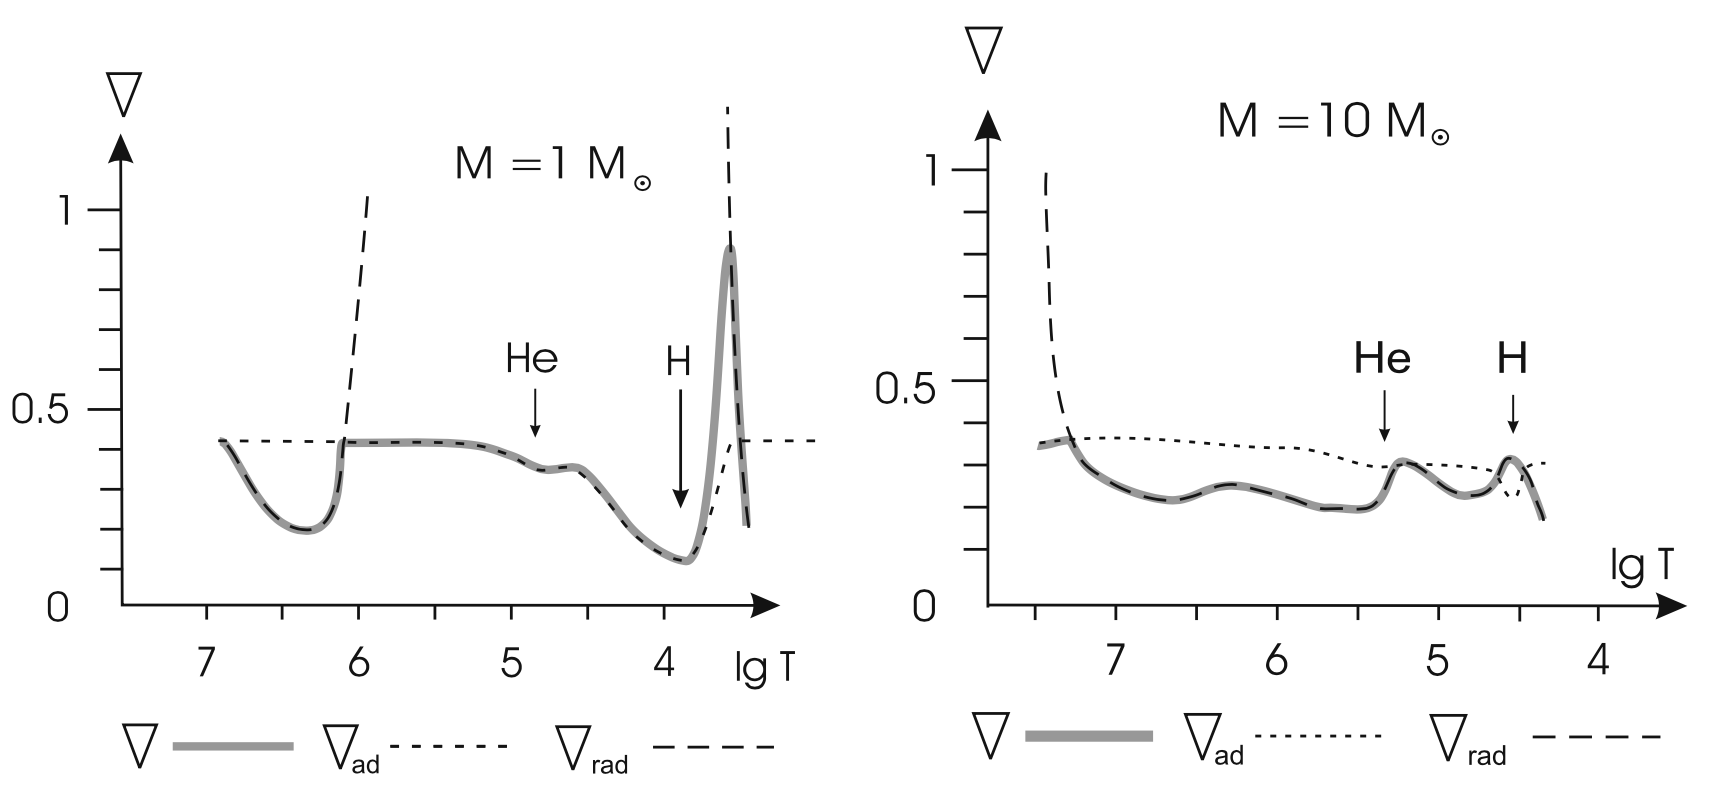
\includegraphics[width=14cm]{figures/DelT.png}
    \caption{\footnotesize{\\The grey solid lines show the actual temperature gradient $\nabla={\rm d}\ln T/{\rm d}\ln P$ over the temperature $T$ (in ${\rm K}$) inside two ZAMS models of $1\,{\rm M_\odot}$ (left panel) and $10\,{\rm M_\odot}$ (right panel). The corresponding adiabatic gradients $\nabla_{\rm ad}$ (dotted lines) and radiative gradients $\nabla_{\rm rad}$ (dashed lines) are also plotted, and the location of the ionization zones of hydrogen and helium are indicated (arrows). The chemical composition of the models is the same as for those of Figure \ref{fig:convectiveregions}. Figure taken from Kippenhahn, Weigert \& Weiss (2012).}}
    \label{fig:delT}
\end{figure}

{\noindent}Outer convective envelopes can generally be expected to occur in stars of low effective temperature. When studying the different gradients in the outer layers of cool stars (Figure \ref{fig:delT}a), one finds a variety of complicated details. The variation of $\nabla_{\rm ad}$ clearly shows depressions in those regions where the most abundant elements, hydrogen ($T\gtrsim10^4\,{\rm K}$) and helium ($T\approx10^5\,{\rm K}$), are partially ionized. The most striking feature is that $\nabla_{\rm rad}$ reaches enormous values (more than $10^5$. This is due to the large opacity $\kappa$, which here increases by several powers of 10. Therefore the Schwarzschild criterion indicates convective instability: the models have an outer convective zone. In the largest part of it, the density is so high that convection is very effective and the actual gradient $\nabla$ is close to $\nabla_{\rm ad}$. Convective transport becomes ineffective only in the outermost, super-adiabatic part, where $\nabla$ is clearly above $\nabla_{\rm ad}$. Scarcely anything of all these features appears in the hot envelope of the $10\,{\rm M_\odot}$ star (Figure \ref{fig:delT}b). $\nabla_{\rm rad}$ remains nearly at the same level; even the photosphere is too hot for hydrogen to be neutral, and only the small dip from the second He ionization is seen immediately below the photosphere. This causes such a shallow zone with convective instability that only for special cases, depending on the detailed chemical composition, convective motions set it.

{\noindent}The outer convection zone gradually penetrates deeper into the star with decreasing $T_{\rm eff}$. Its lower border finally reaches the centre at $M\lesssim0.25\,{\rm M_\odot}$ (left end of Figure \ref{fig:convectiveregions}), such that the main-sequence stars of even smaller masses are fully convective.

{\noindent}\textbf{The present-day interior structure of the Sun}: Consistent with the current age of the Sun, a \textbf{solar model} may be constructed for the present-day Sun. Table \ref{table:solarconditions} gives the values of the central temperature, pressure, density, and composition for one such solar model, and a schematic diagram of the model is shown in Figure \ref{fig:solarinterior}. According to the evolutionary sequence leading to this model, during its lifetime the mass fraction of hydrogen ($X$) in the Sun's center has decreased from its initial value of $0.71$ to $0.34$, while the central mass fraction of helium ($Y$) has increased from $0.27$ to $0.64$. In addition, due to diffusive settling of elements heavier than hydrogen, the mass fraction of hydrogen near the surface has increased by approximately $0.03$, while the mass fraction of helium has decreased by $0.03$.

\begin{table}[t]
\floatbox[\capbeside\thisfloatsetup{capbesideposition={right,top},capbesidewidth=5cm}]{table}
{\caption{Central conditions in the Sun. (Data from Bahcall, Pinsonneault, and Basu, Ap. J., 555, 990, 2001.) Table taken from Carrol \& Ostlie (2007).}\label{table:solarconditions}}%
{\begin{tabular}{ll}
\hline
 Temperature & $1.57\times10^7{\rm K}$ \\
 Pressure    & $2.342\times10^{16}\,{\rm N\,m^{-2}}$ \\
 Density     & $1.527\times10^5\,{\rm kg\,m^{-3}}$ \\
 $X$         &  $0.3397$ \\
 $Y$         & $0.6405$ \\
 \hline
\end{tabular}}
\end{table}

\begin{figure}[t]
    \floatbox[{\capbeside\thisfloatsetup{capbesideposition={right,top},capbesidewidth=4cm}}]{figure}[\FBwidth]
    {\caption{\footnotesize{\\Figure taken from \href{https://web.njit.edu/~gary/321/Lecture9.html}{https://web.njit.edu/~gary/321/Lecture9.html}.}}
    \label{fig:solarinterior}}
    {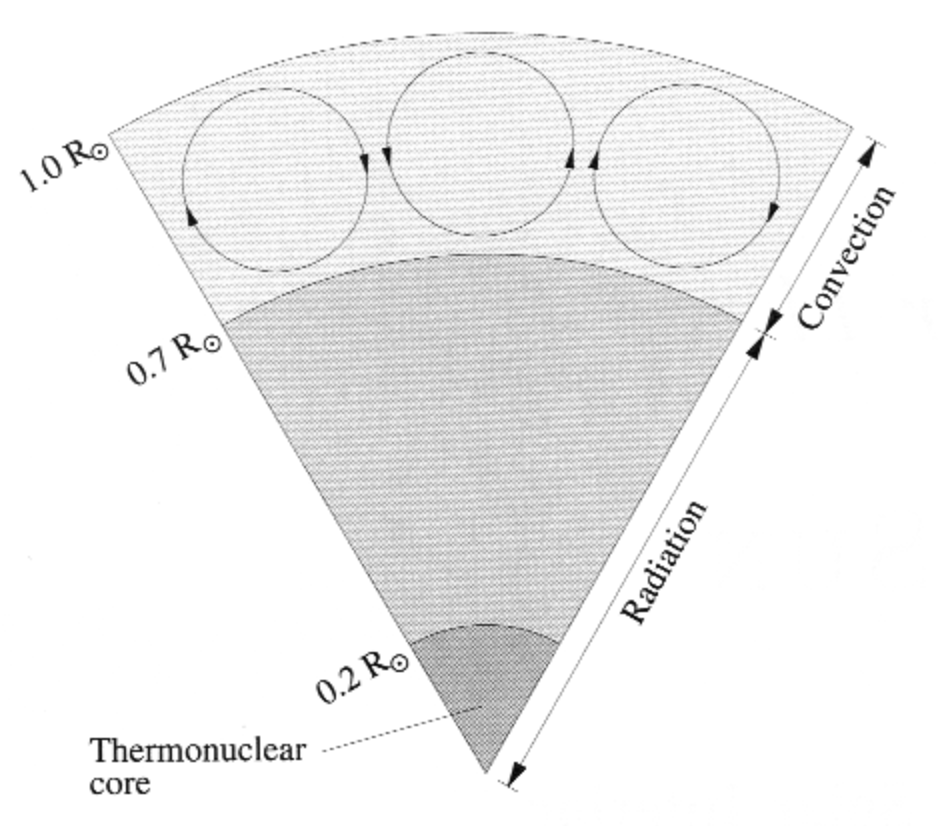
\includegraphics[width=6cm]{figures/SolarInterior.png}}
\end{figure}

{\noindent}Because of the Sun's past evolution, its composition is no longer homogeneous but instead shows the influence of ongoing nucleosynthesis, surface convection, and elemental diffusion (i.e., settling of heavier elements). The composition structure of the Sun is shown in Figure \ref{fig:solarinterior} for $_1^1$H, $^3_2$He, and $^4_2$He. Since the Sun's primary energy production mechanism is the pp chain, $^3_2$He is produced and then destroyed again. At the top of the hydrogen burning region where the temperature is lower, $^3_2$He is relatively more abundant because it is produced more easily than it is destroyed. At greater depths, the higher temperatures allow the $^3_2$He-$^3_2$He interactions to proceed more rapidly, and the $^3_2$He abundance again decreases (the temperature profile of the Sun is shown in Figure \ref{fig:massfracrad}). The slight ramp in the $^1_1$H and $^4_2$He curves near $0.7\,{\rm R_\odot}$ reflects evolutionary changes in the position of the base of the surface convection zone, combined with the effects of elemental diffusion. Within the convection zone, turbulence results in essentially complete mixing and a homogenous composition. The base of the present-day convection zone is at $0.714\,{\rm R_\odot}$.

\begin{figure}[h]
    \floatbox[{\capbeside\thisfloatsetup{capbesideposition={right,top},capbesidewidth=4cm}}]{figure}[\FBwidth]
    {\caption{\footnotesize{\\The abundance of $^1_1$H, $^3_2$He, and $^4_2$He as a function of radius for the Sun. Note that the abundance of $^3_2$He is multiplied by a factor of $100$. (Data from Bahcall, Pinsonneault, \& Basu, Ap. J., 555, 990, 2001.) Figure adapted from Carrol \& Ostlie (2007).}}
    \label{fig:massfracrad}}
    {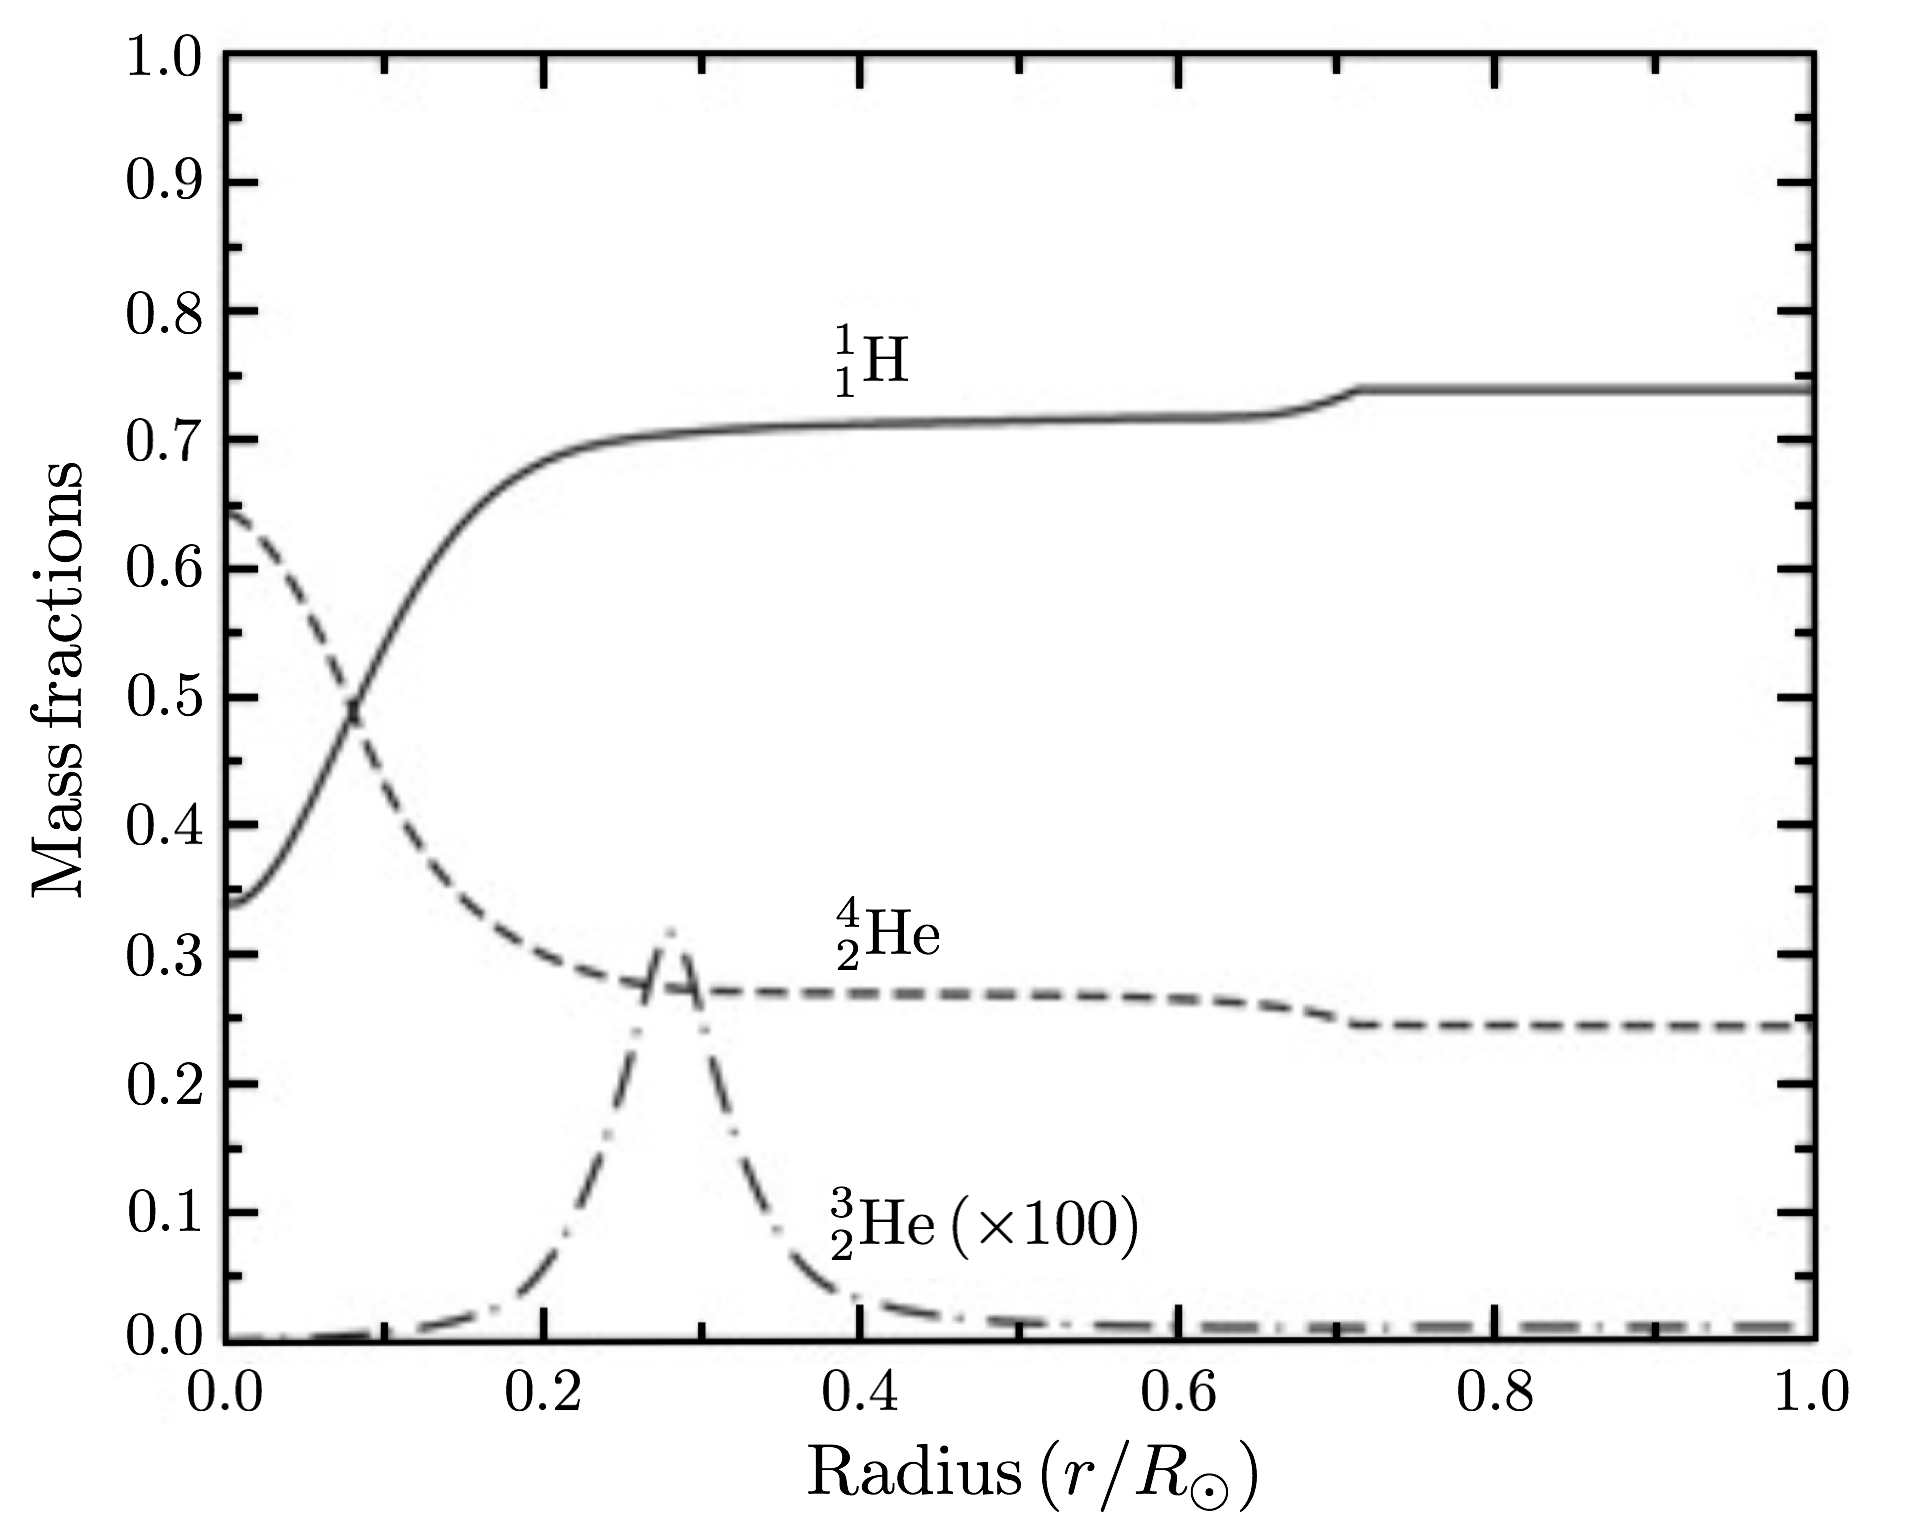
\includegraphics[width=12cm]{figures/MassFractionRadius.png}}
\end{figure}

{\noindent}Figure \ref{fig:solarconvection} shows ${\rm d}\ln P/{\rm d}\ln T$ versus $r/{\rm R_\odot}$. As can be seen, the Sun is purely radiative below $r/{\rm D_\odot}=0.714$ and becomes convective above that point. Physically this occurs because the opacity in the outer portion of the Sun becomes large enough to inhibit the transport of energy by radiation; recall that the radiative temperature gradient is proportional to the opacity:

\begin{align*}
    \frac{{\rm d}T}{{\rm d}r} = -\frac{3}{4ac}\frac{\bar{\kappa}\rho}{T^3}\frac{L_r}{4\pi r^2} ~ [{\rm K\,m^{-1}}].
\end{align*}

{\noindent}When the temperature gradient becomes too large, convection becomes the more efficient means of energy transport. Throughout most of the region of convective energy transport, ${\rm d}\ln P/{\rm d}\ln T\simeq2.5$, which is characteristic of the nearly adiabatic temperature gradient of most convection zones. The rapid rise in ${\rm d}\ln P/{\rm d}\ln T$ above $0.95\,{\rm R_\odot}$ is due to the significant departure of the actual temperature gradient from the adiabatic one. In this case convection must be described by a more detailed treatment, such as \textbf{mixing length theory}.

\begin{figure}[h]
    \floatbox[{\capbeside\thisfloatsetup{capbesideposition={right,top},capbesidewidth=4cm}}]{figure}[\FBwidth]
    {\caption{\footnotesize{\\The convection condition ${\rm d}\ln P/{\rm d}\ln T$ plotted versus $r/{\rm R_\odot}$. The dashed horizontal line represents the boundary between adiabatic convection and radiation for an ideal monatomic gas. The onset of convection does not exactly agree with the ideal adiabatic case because of the incorporation of a sophisticated equation of state and a more detailed treatment of convection physics. The rapid rise in ${\rm d}\ln P/{\rm d}\ln T$ near the surface is associated with a highly super-adiabatic nature of convection in that region (i.e., the adiabatic approximation that convection occurs when ${\rm d}\ln P/{\rm d}\ln T<2.5$ is invalid near the surface of the Sun.) [${\rm d}\ln P/{\rm d}\ln T$ was computed using data from Bahcall, Pinsonneault, and Basu, Ap. J., 555, 990, 2001. The data for the zones above $0.95\,{\rm R_\odot}$ are from Cox, Arthur N. (editor), Allen's Astrophysical Quantities, Fourth Edition, AIP Press, New York, 2000.] Figure adapted from Carrol \& Ostlie (2007).}}
    \label{fig:solarconvection}}
    {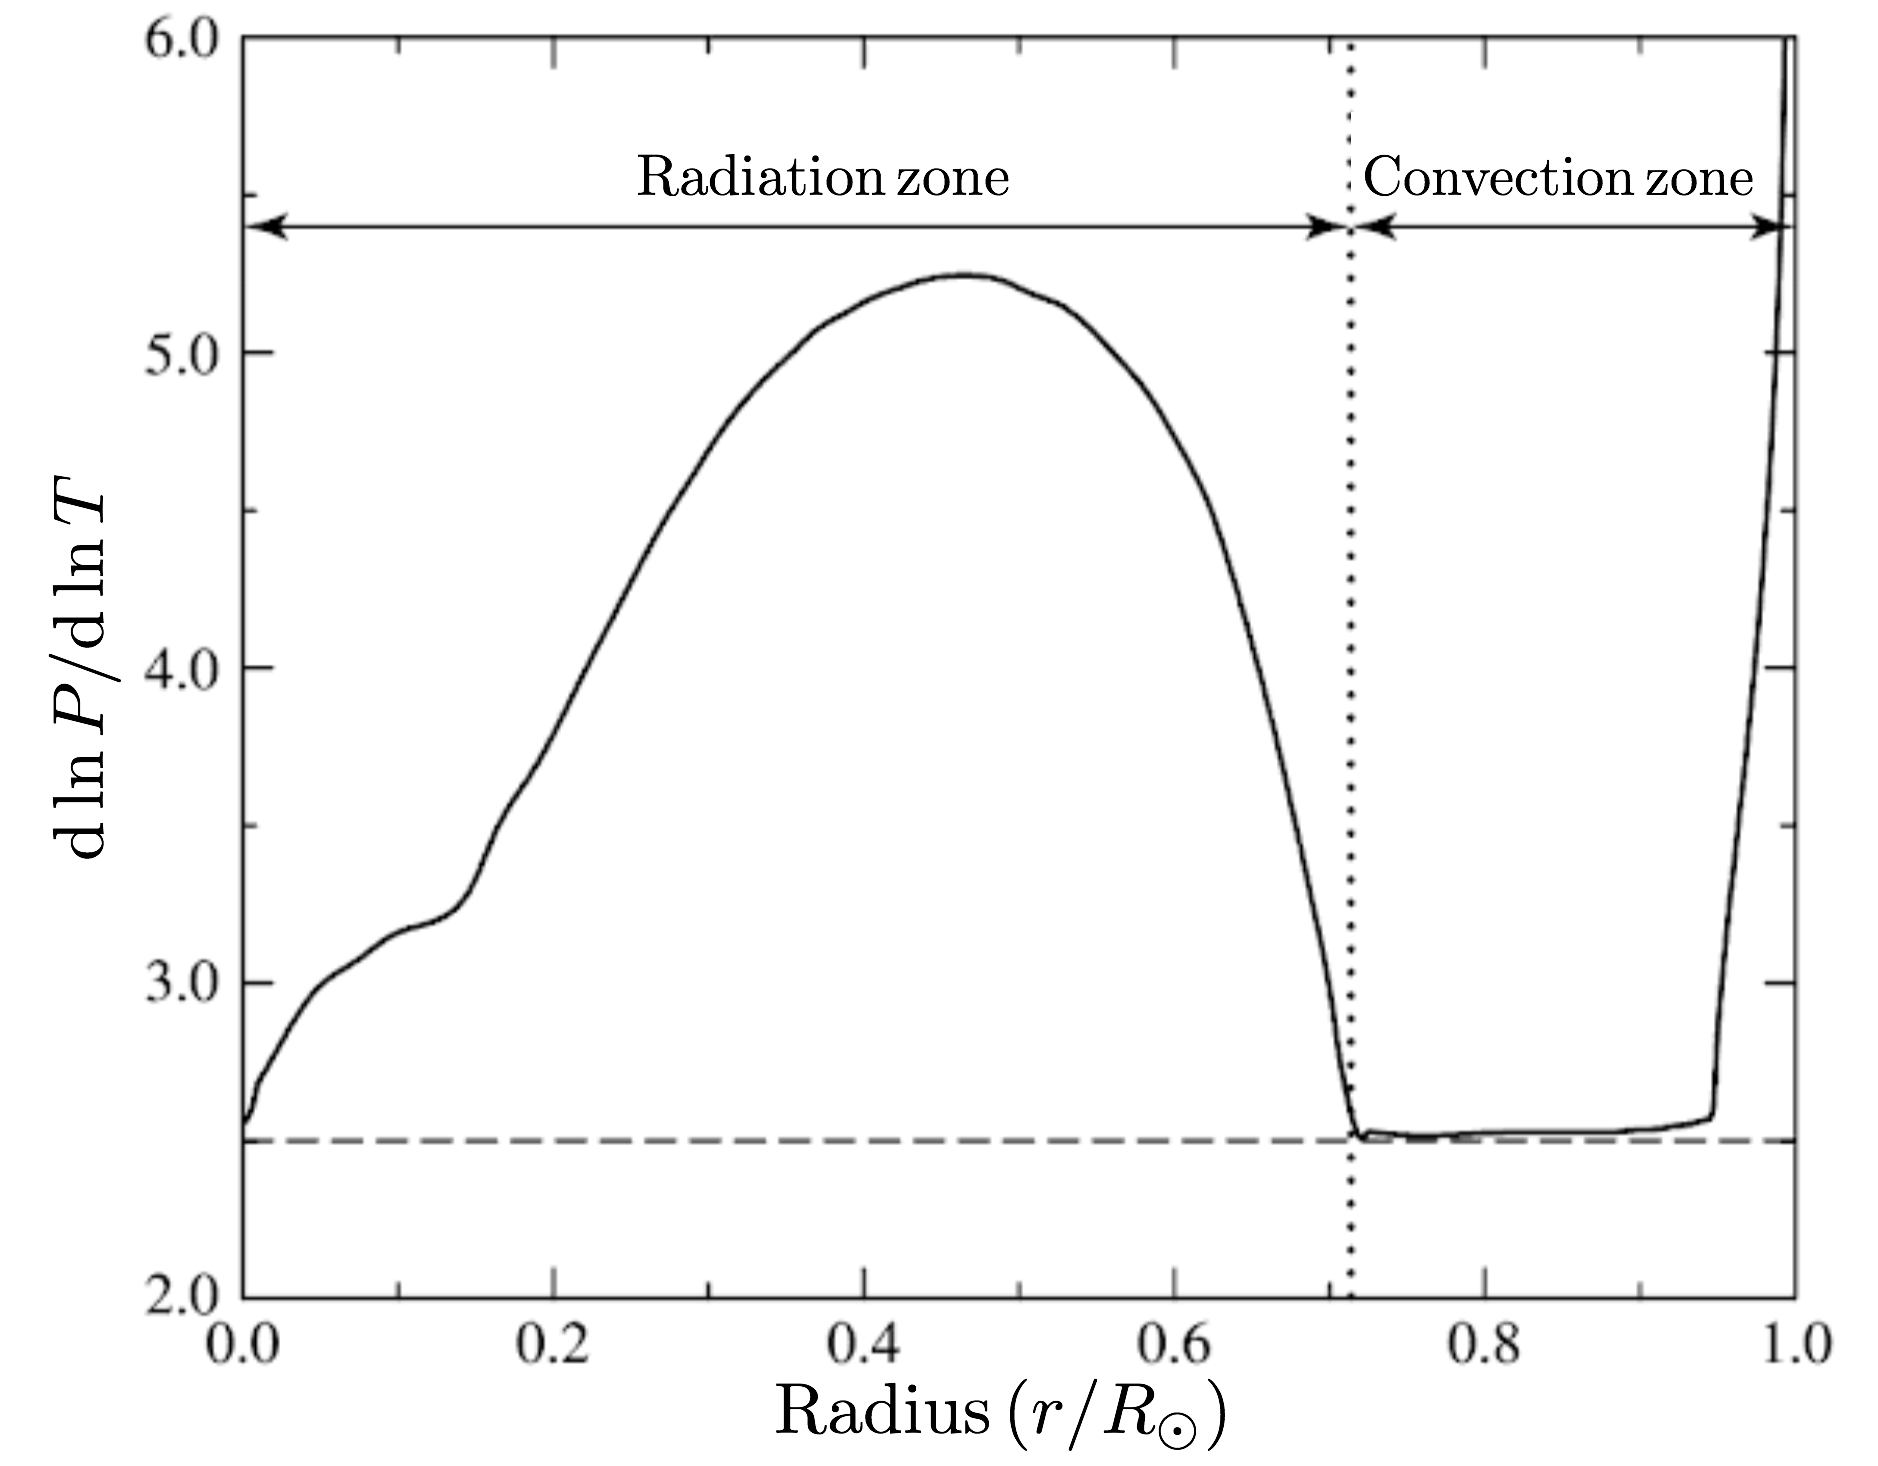
\includegraphics[width=12cm]{figures/SolarConvection.png}}
\end{figure}

{\noindent}Notice that ${\rm d}\ln P/{\rm d}\ln T$ also decreases to almost $2.5$ at the center of the Sun. Although the Sun remains purely radiative at the center, the large amounts of energy that must be transported outward pushes the temperature gradient in the direction of becoming super-adiabatic. Stars only slightly more massive than the Sun are convective in their centers because of the stronger temperature dependence of the CNO cycle as compared to the pp chain. 

\subsubsection{Follow-up Questions}

\begin{itemize}
    \item How do we know that the Sun's outer envelope is convective?
    \item How far into the surface of the Sun does the convective zone permeate? How can we measure this?
\end{itemize}

% --------------------------------------------------------------
%               9. 
% --------------------------------------------------------------

\newpage
\subsection{Question 9}

What is Eddington's luminosity limit? Explain why this limit is important for the properties and lifetimes of massive stars.

\subsubsection{Short answer}

The Eddington luminosity limit is the luminosity limit where the radiative force is balanced by the gravitational force. This limit is important for the properties and lifetimes of massive stars because stars massive enough to reach such luminosities can have their properties and lifetimes affected; at such high luminosities, stellar material can become unbound and ejected from the stellar surface via stellar winds.

\subsubsection{Additional context}

Sir Arthur Stanley Eddington observed that radiation and gravitation both obey inverse-square laws and so there would be instances when the two forces could be in balance irrespective of distance. Thus there should exist a maximum luminosity for a star of a given mass, where the force of radiation on the surface material would exactly balance the force of gravity.

{\noindent}There exists a gradient of the radiation pressure

\begin{align*}
    \frac{{\rm d}P_{\rm rad}}{{\rm d}r} = \frac{a}{3}T^3\frac{{\rm d}T}{{\rm d}r} ~ [{\rm P\,m^{-1}}],
\end{align*}

{\noindent}which exerts, just like the gas pressure gradient, an outward acceleration (${\rm d}P_{\rm rad}/{\rm d}r<0$)

\begin{align*}
    g_{\rm rad} = -\frac{1}{\rho} \frac{{\rm d}P_{\rm rad}}{{\rm d}r} ~ [{\rm m\,s^{-2}}]
\end{align*}

{\noindent}Using 

\begin{align*}
    F = -\frac{4ac}{3} \frac{T^3}{\kappa\rho}\frac{\partial T}{\partial r} ~ [{\rm erg\,s^{-1}\,cm^{-2}}]
\end{align*}

we see that we can rewrite this as

\begin{align*}
    g_{\rm rad} = \frac{\kappa F_{\rm rad}}{c} = \frac{\kappa L_r}{4\pi r^2c} ~ [{\rm m\,s^{-2}}].
\end{align*}

{\noindent}In case that radiation pressure completely dominates over gas pressure, a star can no longer be in hydrostatic equilibrium if $g_{\rm rad}>g$. The sum of both accelerations can be written as

\begin{align*}
    g+g_{\rm rad} = -\frac{Gm}{r^2} \left[ 1-\frac{\kappa L_r}{4\pi cGm} \right] = -\frac{Gm}{r^2}[1-\Gamma_r] ~ [{\rm m\,s^{-2}}],
\end{align*}

{\noindent}where $\Gamma_r$ can be understood as the ratio of the luminosity relative to the critical luminosity at which the bracket changes sign, and thus the star becomes unbound. For $m=M$ this critical luminosity is called the \textbf{Eddington luminosity} and is

\begin{align*}
    L_E = \frac{4\pi cGM}{\kappa} ~ [{\rm J\,s^{-1}}].
\end{align*}

{\noindent}Expressed in Solar units it is

\begin{align*}
    \frac{L_E}{{\rm L_\odot}} = 1.3\times10^4\frac{1}{\kappa} \frac{M}{{\rm M_\odot}}
\end{align*}

{\noindent}and grows linearly with stellar mass. Since $L\propto M^3$, stars obviously reach a limit, where radiation pressure is able to drive a strong stellar wind, and which depends on the opacity.

{\noindent}For hot, massive stars electron scattering is the dominating opacity source, which can be approximated by

\begin{align*}
    \kappa_\nu &= \frac{8\pi}{3} \frac{e_e^2}{\mu_em_u} \\
    &= 0.20(1+X) ~ [{\rm cm^2\,g^{-1}}],
\end{align*}

and is $\kappa_{\rm sc}=0.20(1+X)$. For a mass fraction of hydrogen of $0.70$ this simplifies to

\begin{align*}
    \frac{L_E}{{\rm L_\odot}} = 3.824\times10^4\frac{M}{{\rm M_\odot}}.
\end{align*}

{\noindent}For $M\approx200\,{\rm M_\odot}$ the luminosity of massive main-sequence stars reach the Eddington limit and disperse. This is a rough estimate for an upper limit. In reality the instability of this mechanism occurs at lower mass. However, the Eddington limit can become quite important in other situations.

{\noindent}Any object that has a luminosity greater than $L_E$ will be forced into instability by its own radiation pressure. This effectively provides a mass-luminosity relationship for super-massive stars since these radiation-dominated configurations will radiate near their limit. It is worth noting that \textbf{magnetars}, the source for \textbf{soft gamma repeaters}, are class of gamma-ray bursts that \textit{exceed the Eddington luminosity by far}, but are characterized by a comparably soft gamma spectrum. In a magnetar, the decaying magnetic field is the source of free energy (rather than rotation, as in pulsars).

{\noindent}\textbf{Limiting masses for super-massive stars}: Any star with a mass less than about half a million solar masses can come to equilibrium burning hydrogen via the CNO cycle, albeit with a short lifetime. More massive stars are destined to continue to contract. Of course, more massive stars will produce nuclear energy at an ever-increasing rate as their central temperatures rise. However, the rate of energy production cannot increase without bound. This is suggested by the declining exponents of the temperature dependence shown in Table \ref{table:tempdependence}. The nuclear reactions that involve β decay set a limit on how fast the CNO cycle can run, and $\beta$ decay is independent of temperature. So there is a maximum rate at which energy can be produced by the CNO cycle operating in these stars.

\begin{table}[h]
    \centering
    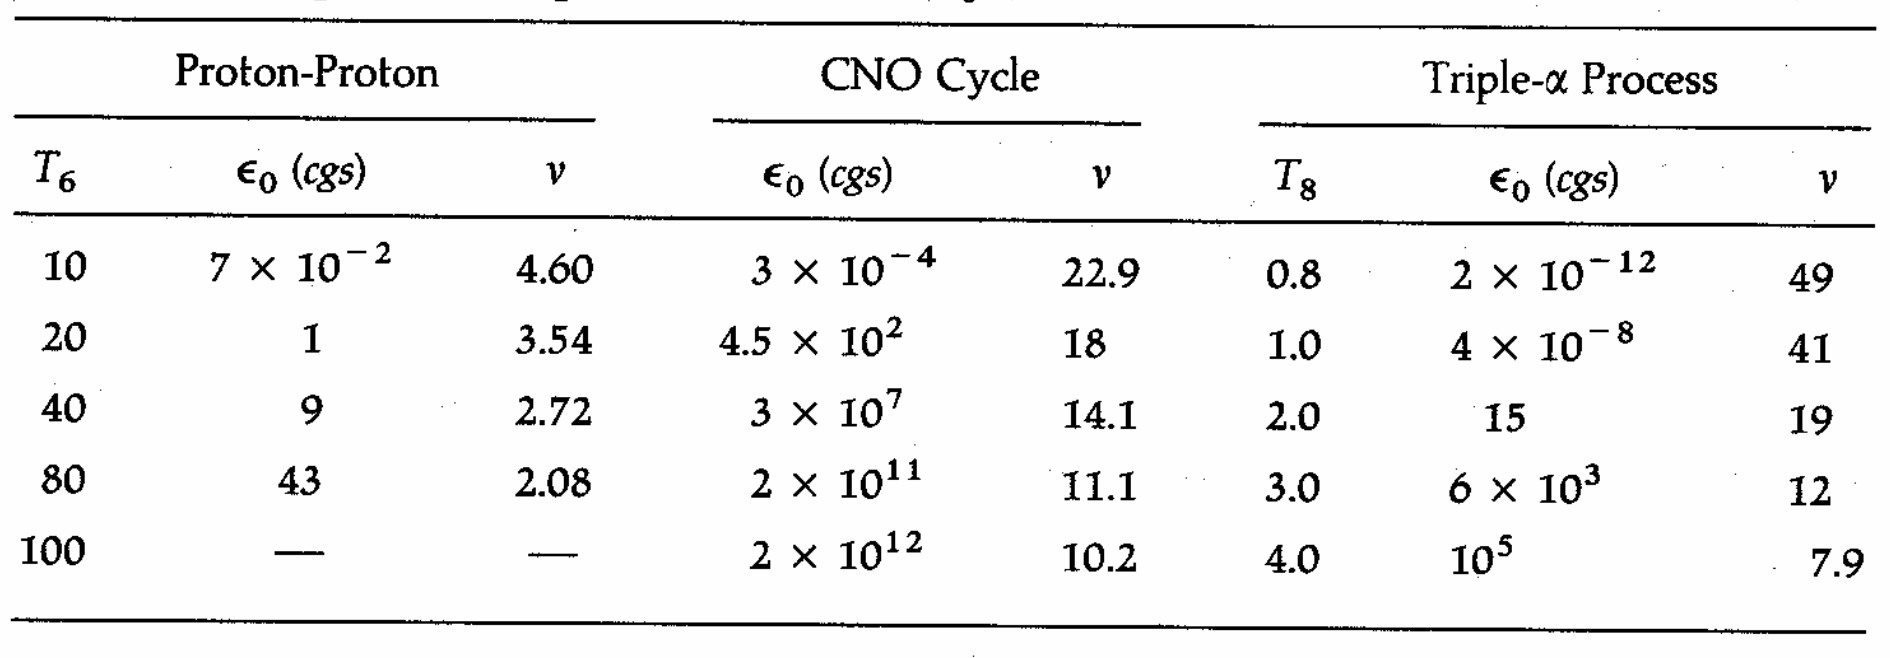
\includegraphics[width=14cm]{figures/TempDependence.png}
    \caption{\footnotesize{Table taken from Collins (2003).}}
    \label{table:tempdependence}
\end{table}

{\noindent}If the nuclear energy produced is sufficient to bring the total energy above the binding energy curve, the star will explode. However, should the energy not be produced at a rate sufficient to catch the binding energy that is rising due to the relativistic collapse, the star will continue an unrestrained collapse to the Schwarzschild radius and become a black hole. Which scenario is played out will depend on the star's mass. For these stars, the temperature gradient will be above the adiabatic gradient, so convection will exist. However, the only energy transportable by convection is the kinetic energy of the gas, which is an insignificant fraction of the internal energy. Therefore, unlike normal main sequence stars, although it is present, convection will be a very inefficient vehicle for the transport of energy. This is why the star remains with a structure of a polytrope of index $n=3$ in the presence of convection. The pressure support that determines the density distribution comes entirely from radiation and is not governed by the mode of energy transport.

{\noindent}The star will radiate at the Eddington luminosity, and that will set the time scale for collapse. The total energy of these stars is small compared to the gravitational energy. So most of the energy derived from gravitational contraction must go into supporting the star, and very little is available to supply the Eddington luminosity. This can be seen from the relativistic Virial theorem which indicates that any change in the gravitational energy is taken up by the kinetic energy. Relativistic particles (in this case, photons) are much more difficult to bind by gravitation than ordinary matter; thus little of the gravitational energy resulting from collapse will be available to let the star shine. The collapse will proceed very quickly on a time scale that is much nearer to the dynamical time scale than the Kelvin-Helmholtz time scale. The onset of nuclear reactions will slow the collapse, but will not stop it for the massive stars.

{\noindent}A dynamical analysis shows that stars more massive than about $7.5\times10^5\,{\rm M_\odot}$ will undergo collapse to a black hole. Here the collapse proceeds so quickly and the gravity is so powerful that the nuclear reactions, being limited by $\beta$ decay at the resulting high temperatures, do not have the time to produce sufficient energy to arrest the collapse. For less massive stars, this is not the case. Stars in the narrow range of $5\times10^5M⊙\leq M\leq 7.5\times10^5\,{\rm M_\odot}$ will undergo explosive nuclear energy generation resulting in the probable destruction of the star.

{\noindent}Nothing has been said about the role of chemical composition in the evolution of these stars. Clearly, if there is no carbon present, the CNO cycle is not available for the stabilization of the star. Model calculations show that the triple-alpha process cannot stop the collapse. For stars with low metal abundance, only the pp-cycle is available as an energy source. This has the effect of lowering the value of the maximum stable mass. Surprisingly, there is no range at which an explosion occurs. If the star cannot stabilize before reaching $R_m$, it will continue in a state of unrestrained gravitational collapse to a black hole. Thus, it seems unlikely that stars more massive than about a half million solar masses could exist. In addition, it seems unlikely that black holes exist with masses greater than a few solar masses and less than half a million solar masses. If they do, they must form by accretion and not as a single entity.

\subsubsection{Follow-up Questions}

\begin{itemize}
    \item Draw a force diagram of what's happening.
    \item What particles experience gravity the most?
    \item What particles experience photon pressure the most?
\end{itemize}

% --------------------------------------------------------------
%               10. 
% --------------------------------------------------------------

\newpage
\subsection{Question 10}

Explain why we know what the Sun's central temperature ought to be, and how we know what it actually is.

\subsubsection{Short answer}

The hydrostatic condition

\begin{align*}
    \frac{\partial P}{\partial r} = -\frac{Gm\rho}{r^2} ~ [{\rm P\,m^{-1}}]
\end{align*}

{\noindent}together with an equation of state for a perfect gas

\begin{align*}
    P = \frac{\rho k_BT}{\mu m_{\rm H}} ~ [{\rm P}]
\end{align*}

{\noindent}enables us to estimate the pressure and the temperature in the interior of a star of given mass and radius.

{\noindent}Let us replace the left-hand side of the equation for hydrostatic equilibrium by an average pressure gradient $(P_0-P_c)/$ where $P_0$ and $P_c$ are the pressures at the surface and at the centre, respectively. On the right-hand side, we can replace $m$ and $r$ by rough mean values $M/2$ and $R/2$, and obtain

\begin{align*}
    P_c \approx \frac{2GM^2}{\pi R^4} ~ [{\rm P}].
\end{align*}

{\noindent}From the equation of state for a perfect gas (our assumption of a perfect gas turns out to be fully justified for these values of $P$ and $T$), and with the mean density

\begin{align*}
    \bar{\rho} = \frac{3M}{4\pi R^3} ~ [{\rm g\,cm^{-3}}],
\end{align*}

{\noindent}we find with $P_c$ that

\begin{align*}
    T_c &= \frac{P_c\mu m_{\rm H}}{\bar{\rho} k_B} ~ [{\rm K}] \\
    &= \frac{\left(\dfrac{2GM^2}{\pi R^4}\right)\mu m_{\rm H}}{\left(\dfrac{3M}{4\pi R^3}\right) k_B} ~ [{\rm K}] \\
    &= \left(\frac{2GM^2}{\pi R^4}\mu m_{\rm H}\right) \cdot \left(\frac{3M}{4\pi R^3}k_B\right)^{-1} ~ [{\rm K}] \\
    &= \left(\frac{2GM^2\mu m_{\rm H}}{\pi R^4}\right) \cdot \left(\frac{4\pi R^3}{3Mk_B}\right) ~ [{\rm K}] \\
    &= \frac{8G\mu m_{\rm H}}{3k_B}\left(\frac{M}{R}\right) ~ [{\rm K}].
\end{align*}

{\noindent}Therefore,

\begin{align*}
    T_c \propto \frac{M}{R} ~ [{\rm K}].
\end{align*}

{\noindent}With the mass and the radius of the Sun ($M_\odot=1.989\times10^{33}\,{\rm g}$, $R_\odot=6.96\times10^{10}\,{\rm cm}$) and with $\mu=0.5$, we find that

\begin{align*}
    T_c &= \frac{8G\mu m_{\rm H}}{3k_B}\left(\frac{1.989\times10^{33}\,{\rm g}}{6.96\times10^{10}\,{\rm cm}}\right) ~ [{\rm K}] \\
    &= 3.1\times10^7 ~ [{\rm K}].
\end{align*}

{\noindent}Modern numerical solutions give $T_c=1.6\times10^7\,{\rm K}$.

\subsubsection{Additional context}

Although the Sun is a very ordinary star of average mass and in a quiet state of MS hydrogen burning, it is a unique object for stellar evolution theorists. For no other star so many quantities are known with comparable accuracy obtained by so many different and independent methods. From Kepler's laws and known distances within the solar system we can derive its mass and radius as well as the total luminosity. This yields the effective temperature by application of the Stefan-Boltzmann law. Neutrino experiments on Earth allow the determination of conditions in the innermost energy producing core. And the art of (helio-)seismology has returned with high accuracy the run of the sound speed throughout most of the solar interior, the helium content of the outer convective envelope, and its depth. These quantities restrict the modelling of the present Sun and allow a comparison with stellar evolution theory at a degree of precision which is almost unique in astrophysics. Table \ref{table:solarquantities} summarizes the fundamental solar parameters and the method to derive them. Note that the rather large uncertainty in the solar mass is the result of the uncertainty in Newton's constant of gravity G. Kepler's third law returns their combination, $GM_\odot$, with a precision of $10^{-7}$!

\begin{table}[t]
    \centering
    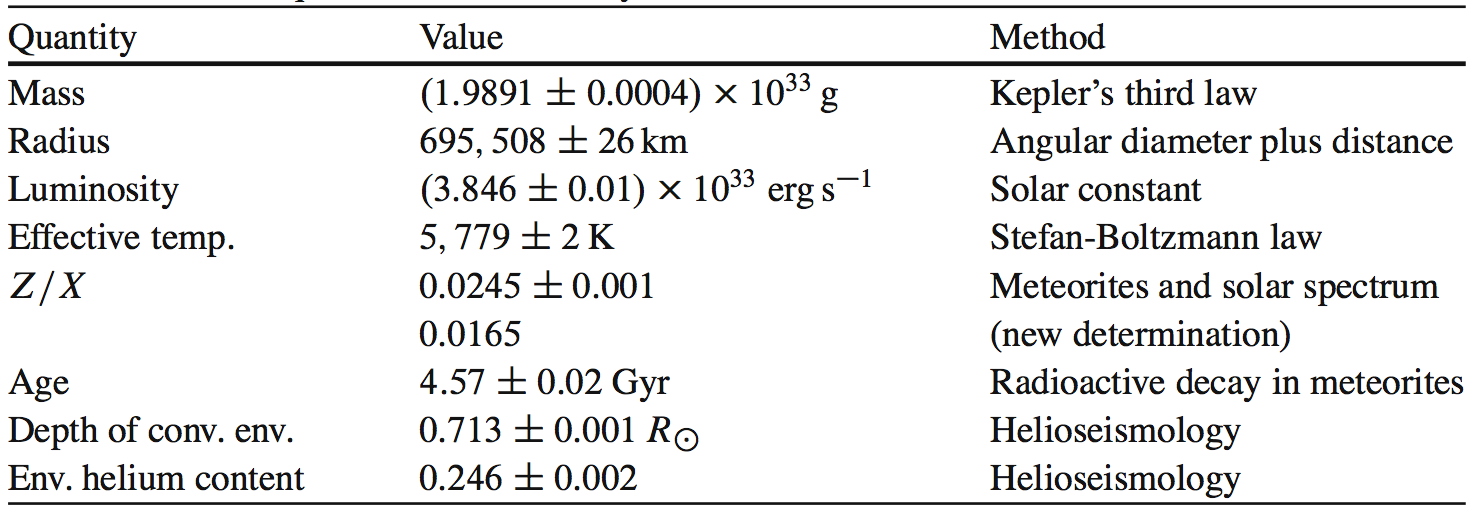
\includegraphics[width=14cm]{figures/SolarQuantities.png}
    \caption{\footnotesize{Solar quantities and how they are derived. Table taken from Kippenhahn, Weigert \& Weiss (2012).}}
    \label{table:solarquantities}
\end{table}

{\noindent}\textbf{Solar neutrinos:} Some of the nuclear reactions of the pp chain, as well as of the CNO cycle, produce neutrinos. In addition, there are also neutrinos due to the very rare \textit{pep} and \textit{hep} reactions

\begin{align*}
    {\rm ^1H+^1H+e^- \rightarrow ^2H+\nu\,(\textit{pep})} \\
    {\rm ^3He+^1H \rightarrow ^4He+e^++\nu\,(\textit{hep})},
\end{align*}

{\noindent}the latter one being the trivial way to produce $^4$He after the \textbf{pp-chain},

\begin{align*}
    {\rm ^1H+^1H \rightarrow ^2H+e^++\nu,} \\
    {\rm ^2H+^1H \rightarrow ^3He+\gamma},
\end{align*}

{\noindent}but it is occurring in only $10^{-8}$ of all cases. However, the energy of the emitted neutrino is close to $10\,{\rm MeV}$, and it is therefore necessary to consider this reaction. The neutrinos leave the star practically without interacting with the stellar matter. The energy spectrum of neutrinos from $\beta$ decay is continuous, since the electrons can take part of the energy away, while neutrinos released after an inverse $\beta$ decay are essentially monochromatic. Therefore most reactions of the pp chain have a continuous spectrum, while the pep-reaction and the electron capture on $^7$Be have a line spectrum. Since $^7$Be can decay into $^7$Li either in the ground state or in an excited state, this reaction gives two spectral lines. The neutrino spectrum of the Sun as predicted from the reactions of the pp chain, computed from our standard solar model, is given in Figure \ref{fig:neutrinospectrum}.

{\noindent}Since the solar neutrinos can leave the Sun almost unimpeded they can in principle be measured in terrestrial laboratories and thus be used to learn directly about conditions in the innermost solar core. This difficult task indeed has been undertaken since 1964, when John Bahcall and Raymond Davies began to plan for an underground neutrino detector in a mine in Homestead, North Dakota. Forty years later the experiments finally have confirmed the standard solar model, and R. Davies received the Nobel Prize for his work. The time in between, however, was characterized by the \textbf{solar neutrino problem}.

{\noindent}The solar neutrino problem consisted in the fact that since the first results from the so-called chlorine experiment by Davies there was a lack of neutrinos compared to solar model predictions. The chlorine experiment is sensitive to neutrinos with energies above $0.814\,{\rm MeV}$ and therefore, as can be seen in Figure \ref{fig:neutrinospectrum} mainly to the $^8$B neutrinos, with some contribution from pep, hep, and $^7$Be neutrinos. The experiment is based on the reaction $^{37}{\rm Cl}+\nu\rightarrow\,^{37}{\rm Ar}$, where the decays of radioactive argon nuclei are counted. The rate of neutrino captures is commonly measured in solar neutrino units (SNU). One SNU corresponds to $10^{-36}$ captures per second and per target nucleus. The predicted counts amount to $7.5\,{\rm SNU}$ for the chlorine experiment, the measurements averaged over several decades to only $2.5\pm0.2\,{\rm SNU}$. The deficit could indicate that the solar centre is cooler than in the models.

{\noindent}To improve the experimental evidence, additional experiments were started. First, another kind of radio-chemical detector using gallium in the detector fluid measured, due to a much lower energy threshold, the majority of neutrinos, including those from the pp-reaction. Later, electron-scattering detectors were developed, which are sensitive to the highest energies only, but which provide directional information about the neutrino source (for these detectors the \textit{hep}-neutrinos of have to be taken into account.). All experiments confirmed that the solar neutrino flux was of the right order of magnitude, and therefore that indeed the Sun shines by the nuclear fusion of hydrogen, but they also consistently measured a deficit of neutrinos. This deficit, however, varied between different kinds of detectors.

{\noindent}With more and more experimental data it became evident that even hypothetical changes to the solar centre cannot solve the problem and that the solution is most likely to be found in the properties of neutrinos. All nuclear reactions emit electron neutrinos, and these are the only ones that were measured in terrestrial experiment, with the exception of the electron-scattering Sudbury Neutrino Observatory (SNO) experiment in Canada, where heavy water (with a high percentage of deuterium isotopes) was used as the detector. Here also reactions with the two other types (flavours) of neutrinos, muon and tau neutrinos can be detected. Summing these and the electron neutrinos up, the total number of detections is completely consistent with the solar model prediction, within a few percent. What created the apparent solar neutrino deficit is the fact that neutrinos can change their flavour, both while travelling through vacuum and more efficiently in the presence of electrons in the solar interior. A similar effect was also confirmed for muon neutrinos arising in the Earth's upper atmosphere from high-energy cosmic radiation, when measured before or after they have travelled through the Earth's interior. The modelling of the solar interior, together with sophisticated experiments, has therefore resulted in new knowledge about fundamental properties of neutrinos. In particular, these so-called \textbf{neutrino oscillations} are possible only if neutrinos have mass.

\begin{figure}[t]
    \floatbox[{\capbeside\thisfloatsetup{capbesideposition={right,top},capbesidewidth=4cm}}]{figure}[\FBwidth]
    {\caption{\footnotesize{The neutrino spectrum of the Sun as predicted from the theoretical standard solar model. The solid lines belong to reactions of the pp chain while the broken lines are due to reactions of the CNO cycle. The neutrinos from most of the reactions have continuous spectra, while mono-energetic neutrinos come from $^7$Be and from the pep-reaction. The flux  for the continuum sources is given in $cm^2\,s^{-1}\,MeV^{-1}$ and for the line sources in $cm^2\,s^{-1}$. The sensitivity of the three types of neutrino experiments is indicated above the figure and by the shaded regions. Figure taken from Kippenhahn, Weigert \& Weiss (2012).}}
    \label{fig:neutrinospectrum}}
    {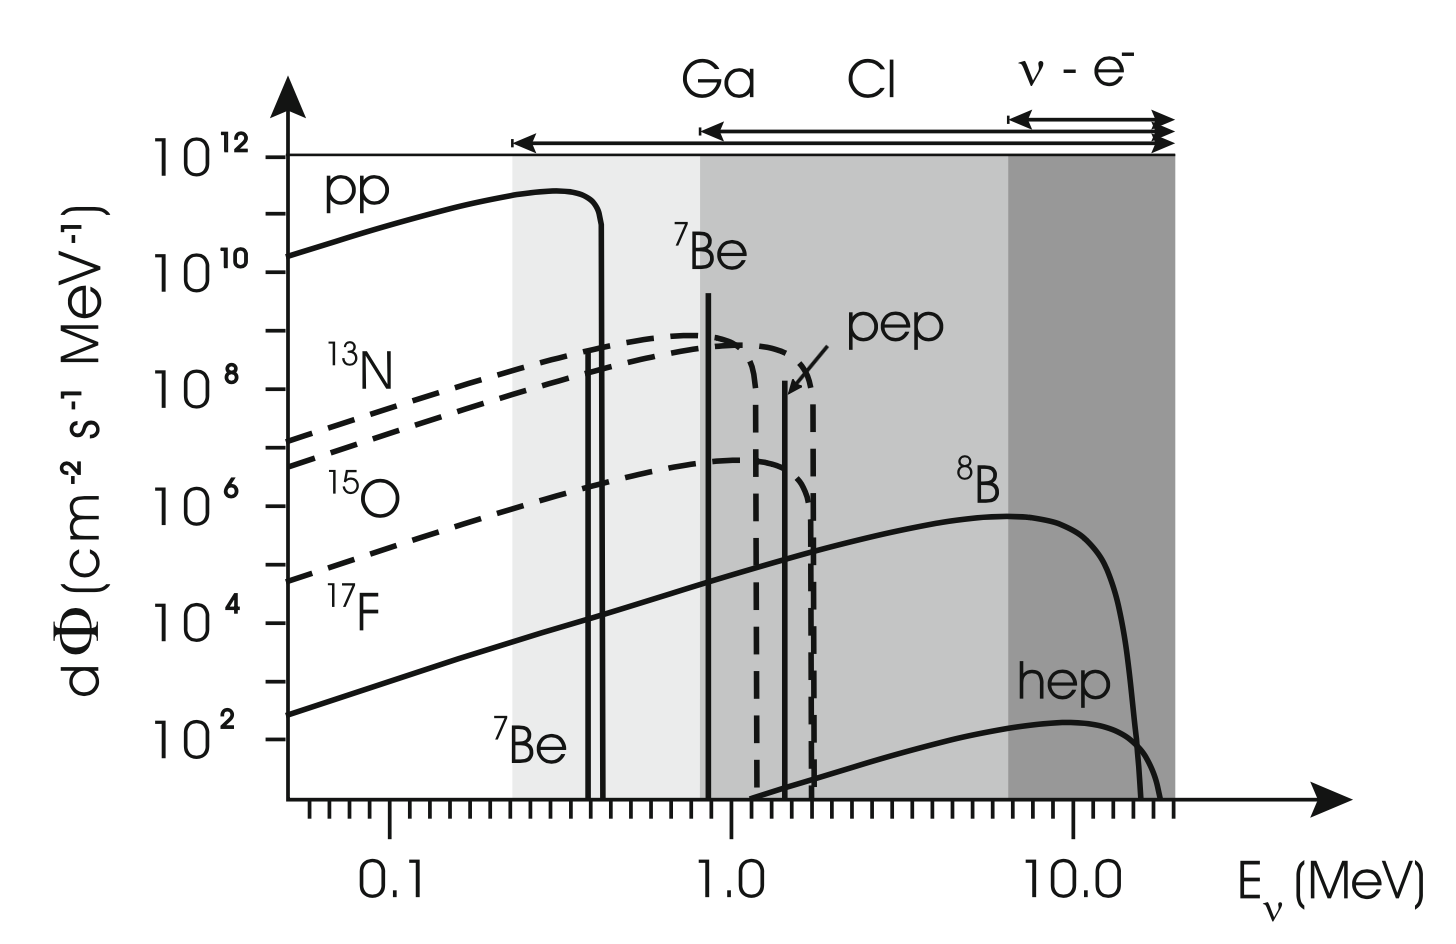
\includegraphics[width=10cm]{figures/NeutrinoSpectrum.png}}
\end{figure}

% --------------------------------------------------------------
%               11. 
% --------------------------------------------------------------

\newpage
\subsection{Question 11}

Which have higher central pressure, high-mass or low-mass main-sequence stars? Roughly, what is their mass-radius relation? Derive this.

\subsubsection{Short answer}

Using hydrostatic equilibrium, we have that:

\begin{align*}
    \frac{{\rm d}P}{{\rm d}r} &= -\frac{GM}{r^2}\rho \\
    P &\sim \frac{M}{R}\rho \\
    P &\sim \frac{M^2}{R^4}.
\end{align*}

{\noindent}With the ideal gas law, we get:

\begin{align*}
    P &= \frac{\rho k_BT}{\mu m_{\rm H}} \\
    P &\sim \rho \\
    P &\sim \frac{M}{R^3}.
\end{align*}

{\noindent}Putting these two together, we get the mass-radius relation:

\begin{align*}
    \frac{M^2}{R^4} &= \frac{M}{R^3} \\
    M &\sim R.
\end{align*}

{\noindent}We can use this to determine the central pressure relation:

\begin{align*}
    P &\sim \frac{M^2}{R^4} \\
    P &\sim \frac{M^2}{M^4} \\
    P &\sim \frac{1}{M^2}.
\end{align*}

{\noindent}Therefore, lower-mass main sequence stars have higher central pressures.

\subsubsection{Follow-up Questions}

\begin{itemize}
    \item How would we actually know the central pressure?
    \item What properties can we measure to test models of stellar structure?
\end{itemize}

% --------------------------------------------------------------
%               12. 
% --------------------------------------------------------------

\newpage
\subsection{Question 12}

Sketch the SED of an O, A, G, M, and T star. Give defining spectral characteristics, such as the Balmer lines and Balmer jump and Calcium doublets, and describe physically.

\subsubsection{Short answer}

{\noindent}Figure \ref{fig:stellarspec_og} shows the spectral sequence from the hottest \textbf{early-type stars}, the O-type stars to spectral type G2. Figure \ref{fig:stellarspec_gm} shows the spectral sequence from the coolest \textbf{late-type} stars, the G2-type stars to spectral type M4.5. Figure \ref{fig:tdwarf} shows the spectrum of a typical mid-T dwarf from the red to the mid-infrared. In the red, the SED is shaped by the very extensive wings of the KI resonance line; in the far red and infrared, the most prominent features are due to CH$_4$ and H$_2$O. Indeed, T dwarfs are distinguished from the L dwarfs by the presence of CH$_4$ absorption in their near-infrared and infrared spectra. All T dwarfs are brown dwarfs.

\begin{figure}[h]
    \centering
    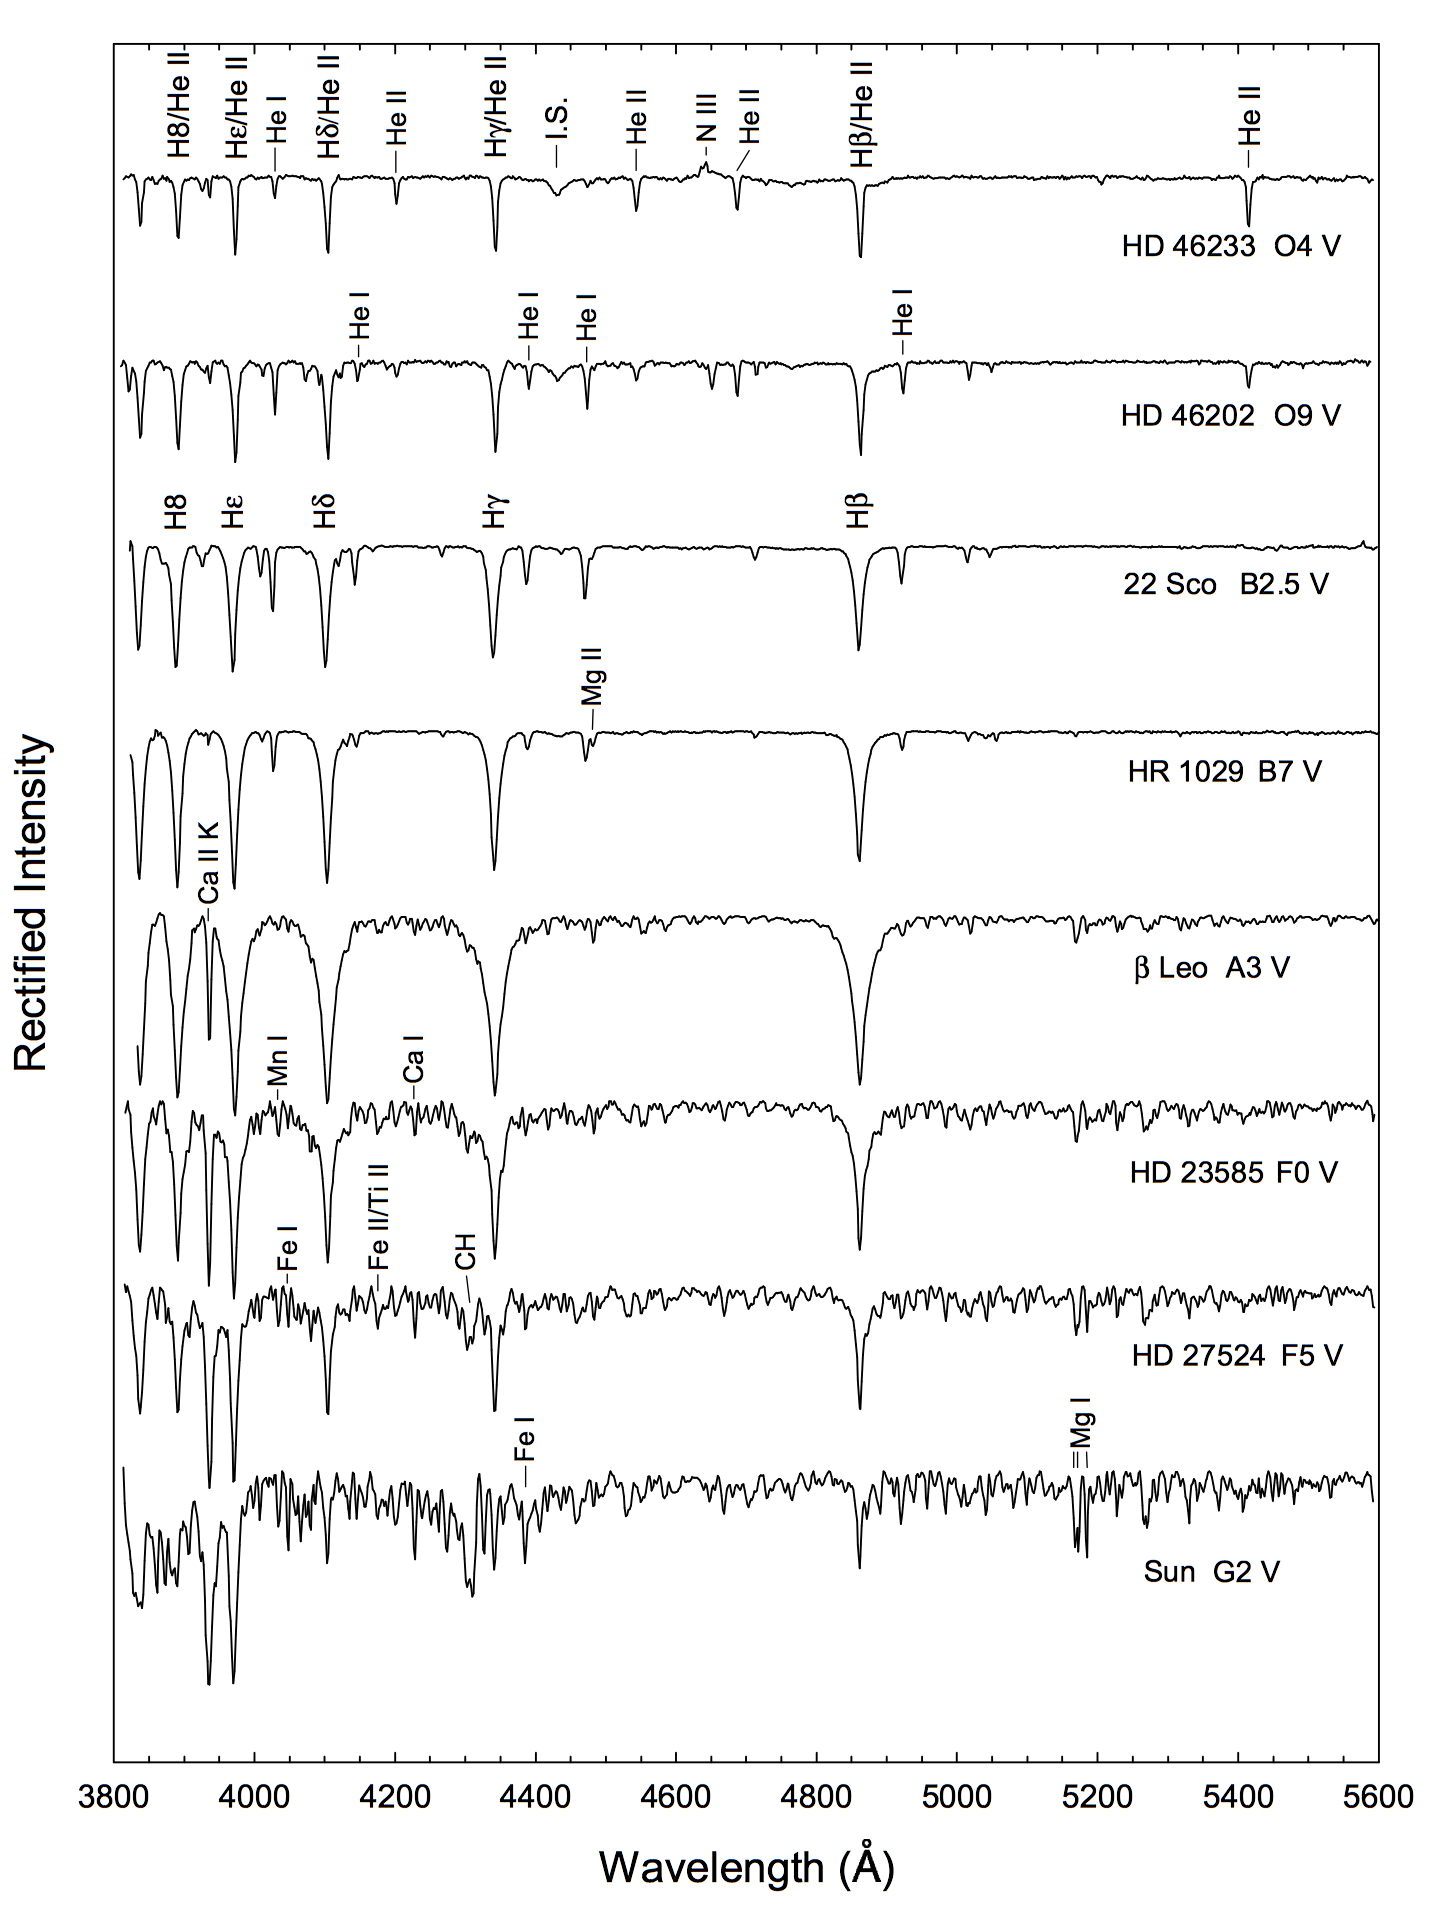
\includegraphics[width=14cm]{figures/StellarSpectra_OG.png}
    \caption{\footnotesize{The Main Sequence from O4 to G2, the ``early-type'' stars. Figure taken from Gray (2009).}}
    \label{fig:stellarspec_og}
\end{figure}

\begin{figure}[h]
    \centering
    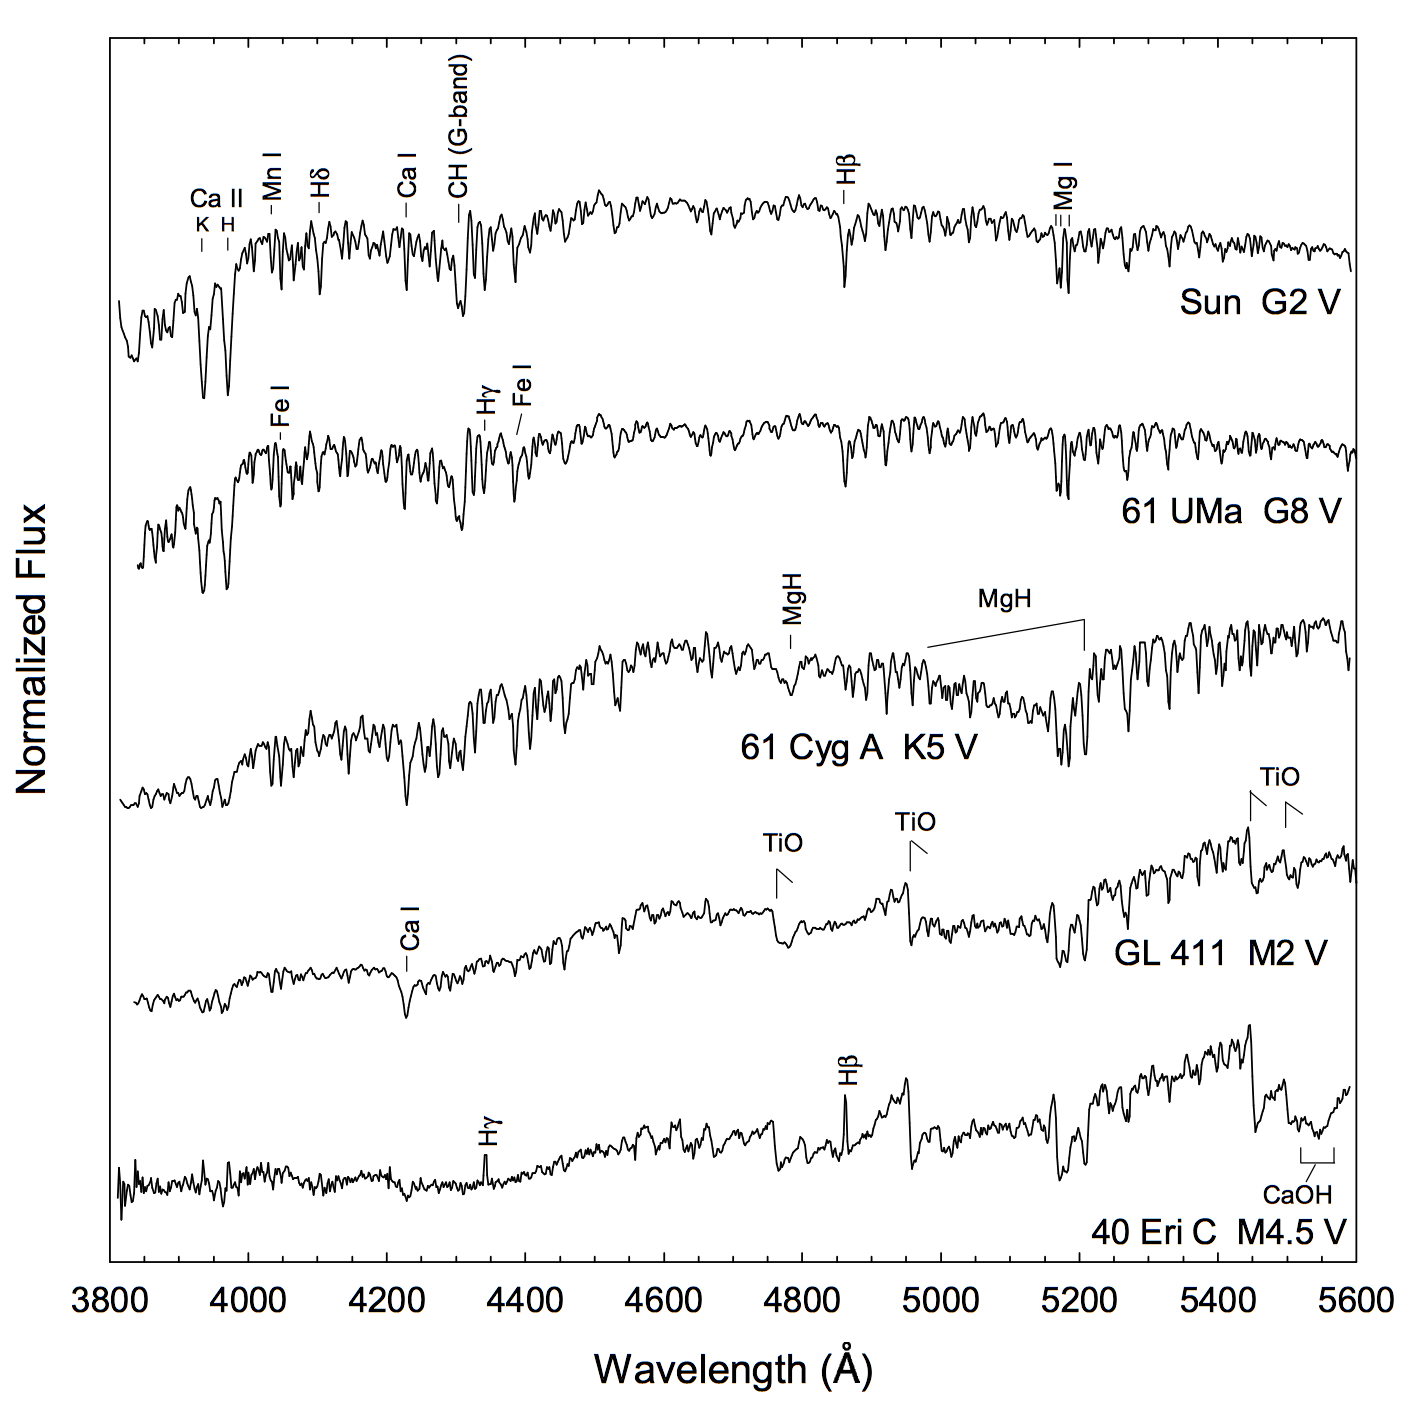
\includegraphics[width=14cm]{figures/StellarSpectra_GM.png}
    \caption{\footnotesize{The Main Sequence from G2 to M4.5, the ``late-type'' stars. Figure taken from Gray (2009).}}
    \label{fig:stellarspec_gm}
\end{figure}

\begin{figure}[h!]
    \centering
    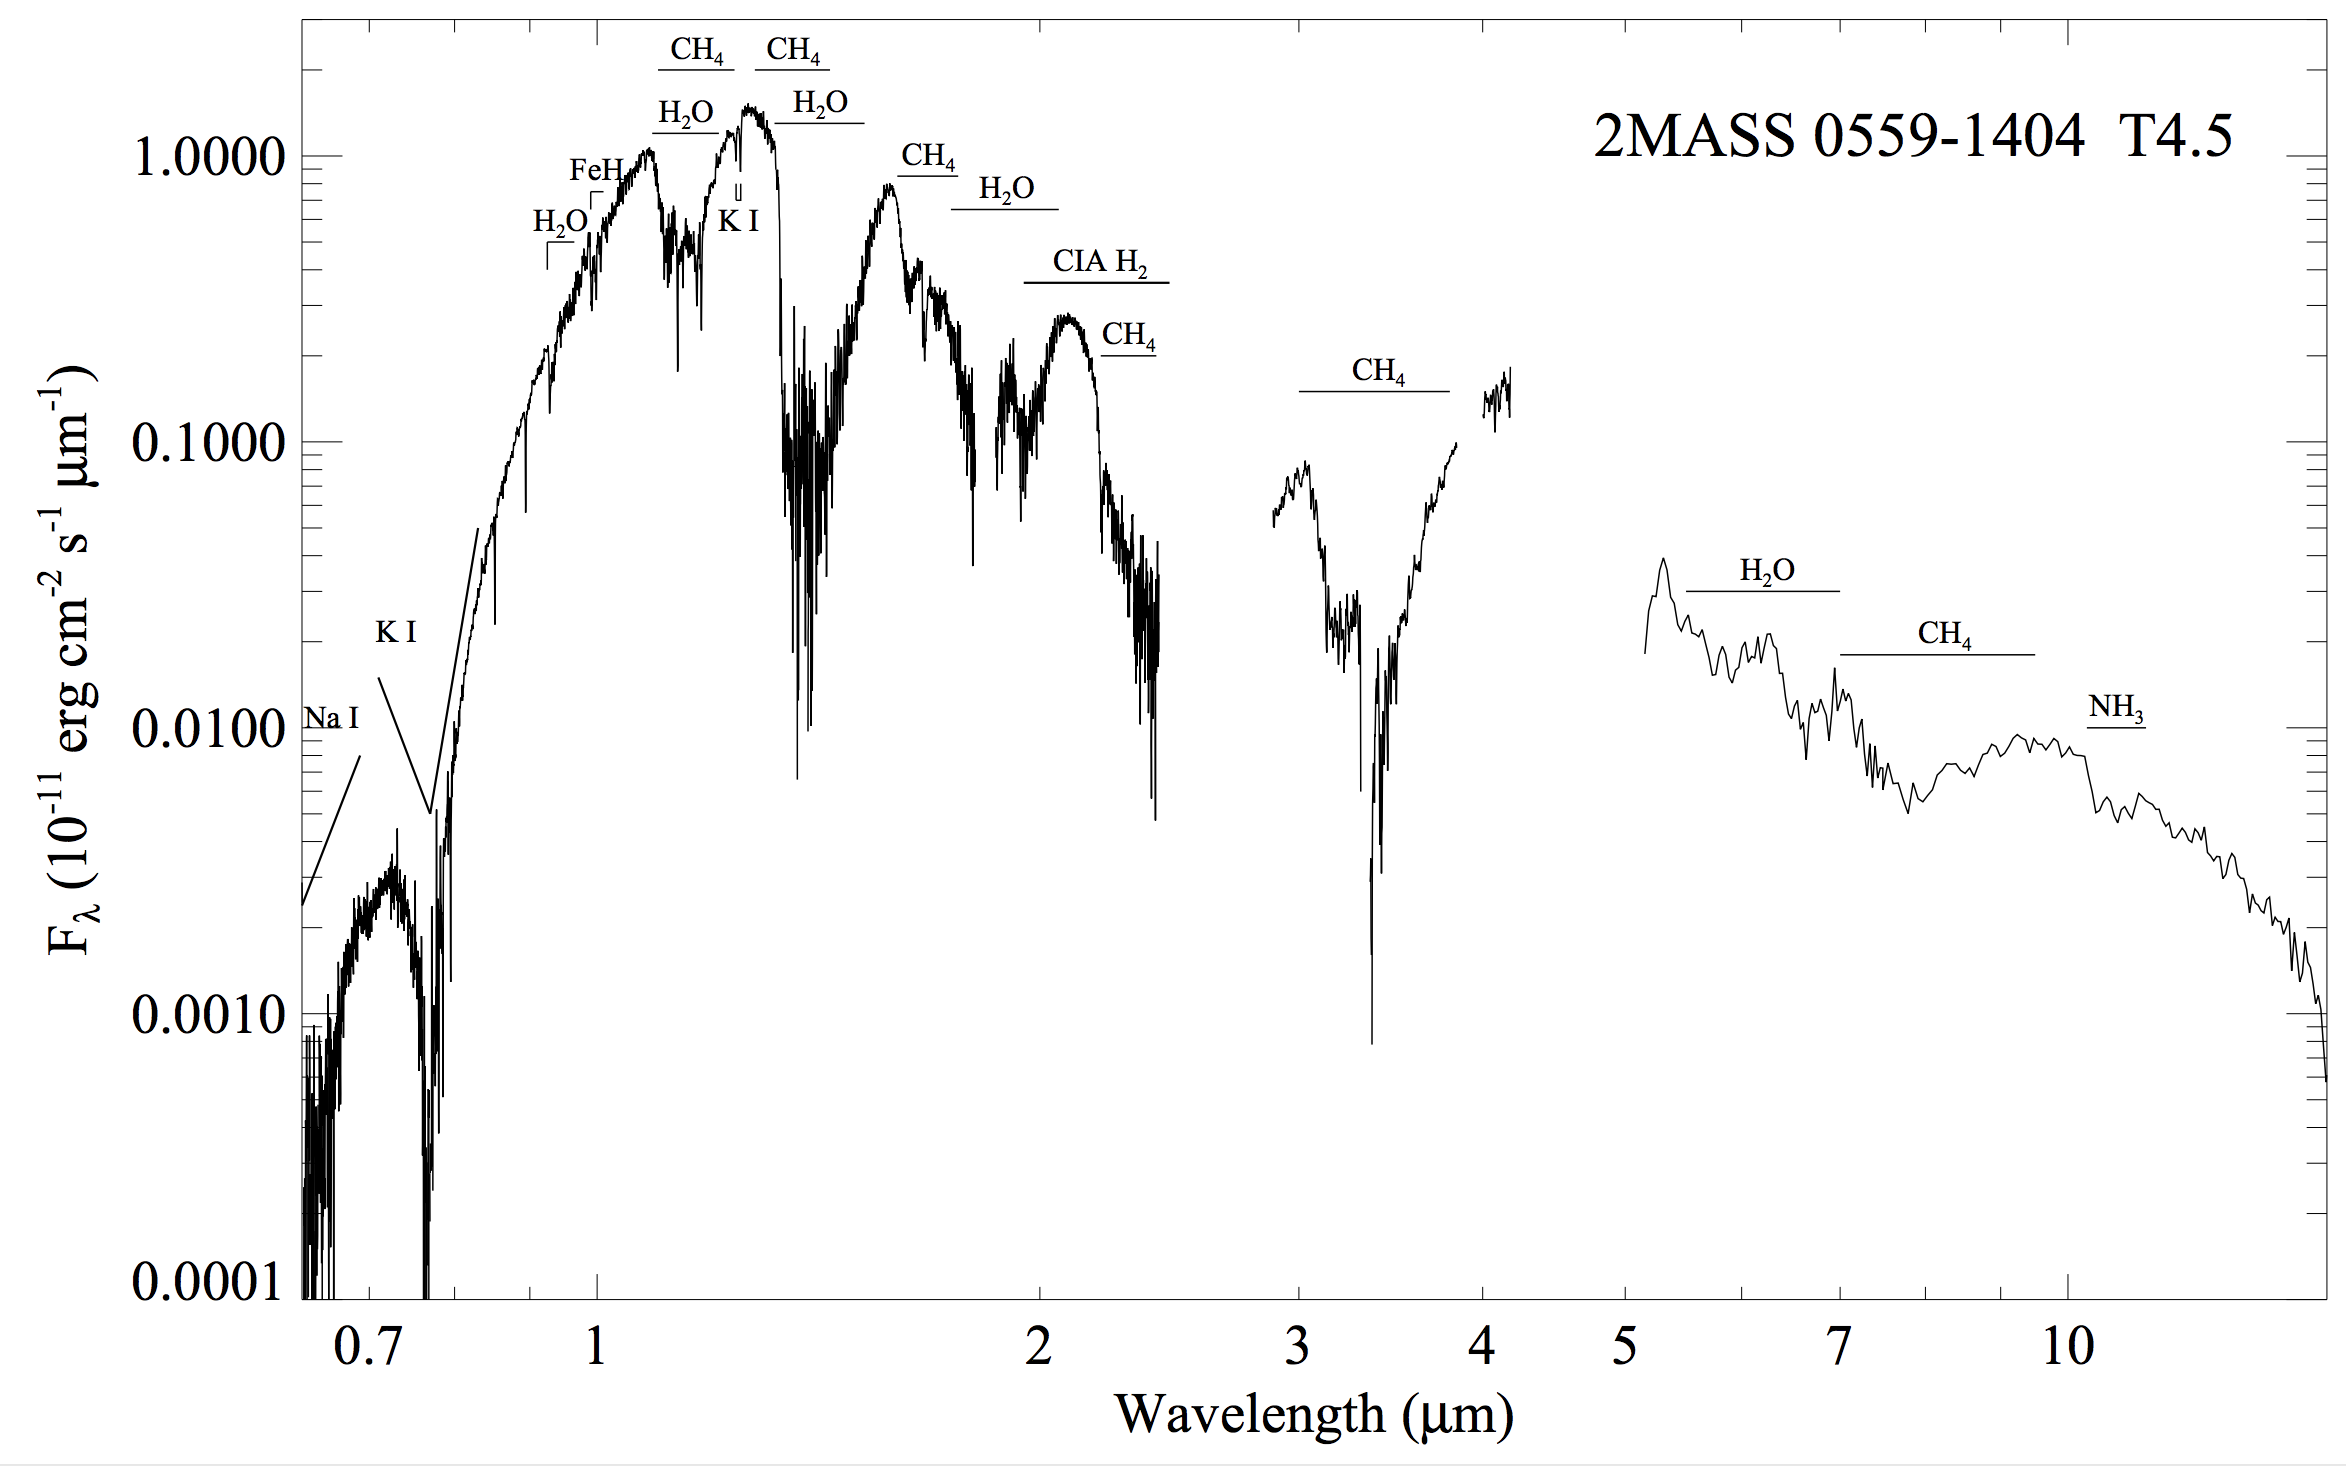
\includegraphics[width=12cm]{figures/Tdwarf.png}
    \caption{\footnotesize{The spectrum of a mid-T dwarf spanning the wavelengths $0.63-15\,\mu{\rm m}$. Prominent atomic and molecular features are labeled. Reproduced from Stellar Spectral Classification, courtesy Adam Burgasser. Figure taken from Gray (2009).}}
    \label{fig:tdwarf}
\end{figure}

\newpage
\subsubsection{Additional context}

The spectra of early-type stars are dominated by the Balmer lines of hydrogen. Note how they increase in strength and reach a maximum at A2, and then fade thereafter. The O- and B-type stars are characterized by lines of helium; the A-, F-, and
G-type stars are characterized by lines of metals. The O-type stars constitute the hottest normal stars, and are characterized by moderately weak hydrogen lines, lines of neutral helium (HeI) and by lines of singly ionized helium (HeII). The spectral type can be judged easily by the ratio of the strengths of lines of HeI to HeII; HeI tends to increase in strength with decreasing temperature while HeII decreases in strength. The ratio HeI $4471$\AA\,to HeII $4542$\AA\,shows this trend clearly. As we move toward later (cooler) types, the helium lines continue to fade until they essentially disappear in spectra of this resolution ($1.8$\AA) at a spectral type of about A0.

{\noindent}The definition of the break between the O-type stars and the B-type stars is the absence of lines of ionized helium (HeII) in the spectra of B-type stars. The lines of HeI pass through a maximum at approximately B2, and then decrease in strength towards later (cooler) types. Were it not for the presence of helium peculiarities in both the early and late B-type stars, the behavior of HeI would be sufficient to accurately estimate the spectral type in the B-type stars. However, because of these peculiarities, the spectral type in the early B-type stars is, instead, estimated on the basis of ratios of lines of silicon ions. For instance, between B0 and B1 (an interval which can be divided into B0, B0.2, B0.5, B0.7 and B1 classes), the SiIV $4089$\AA/SiIII $4552$\AA\,ratio may be used. Between B1 and B3 the SiIII $4552$\AA/SiII $4128.32$\AA\,ratio may be used.

{\noindent}The \textbf{Be stars} are B-type stars that are characterized (or have been characterized in the past) by emission in one or more of the Balmer lines of hydrogen, sometimes accompanied by emission in lines of singly ionized metals, most commonly FeII. The Be class excludes B-type supergiants, as well as pre main-sequence stars such as the Herbig Ae/Be stars. Many Be stars may be classified without difficulty on the MK system, although the more extreme present significant difficulties. An extension to the MK system was introduced for the Be stars comprised of an \textbf{e index} (e1 $\rightarrow$ e4, in direction of increasing emission-line strength). Some typical Be spectra are illustrated in Figure \ref{fig:be}.

\begin{figure}[h]
    \centering
    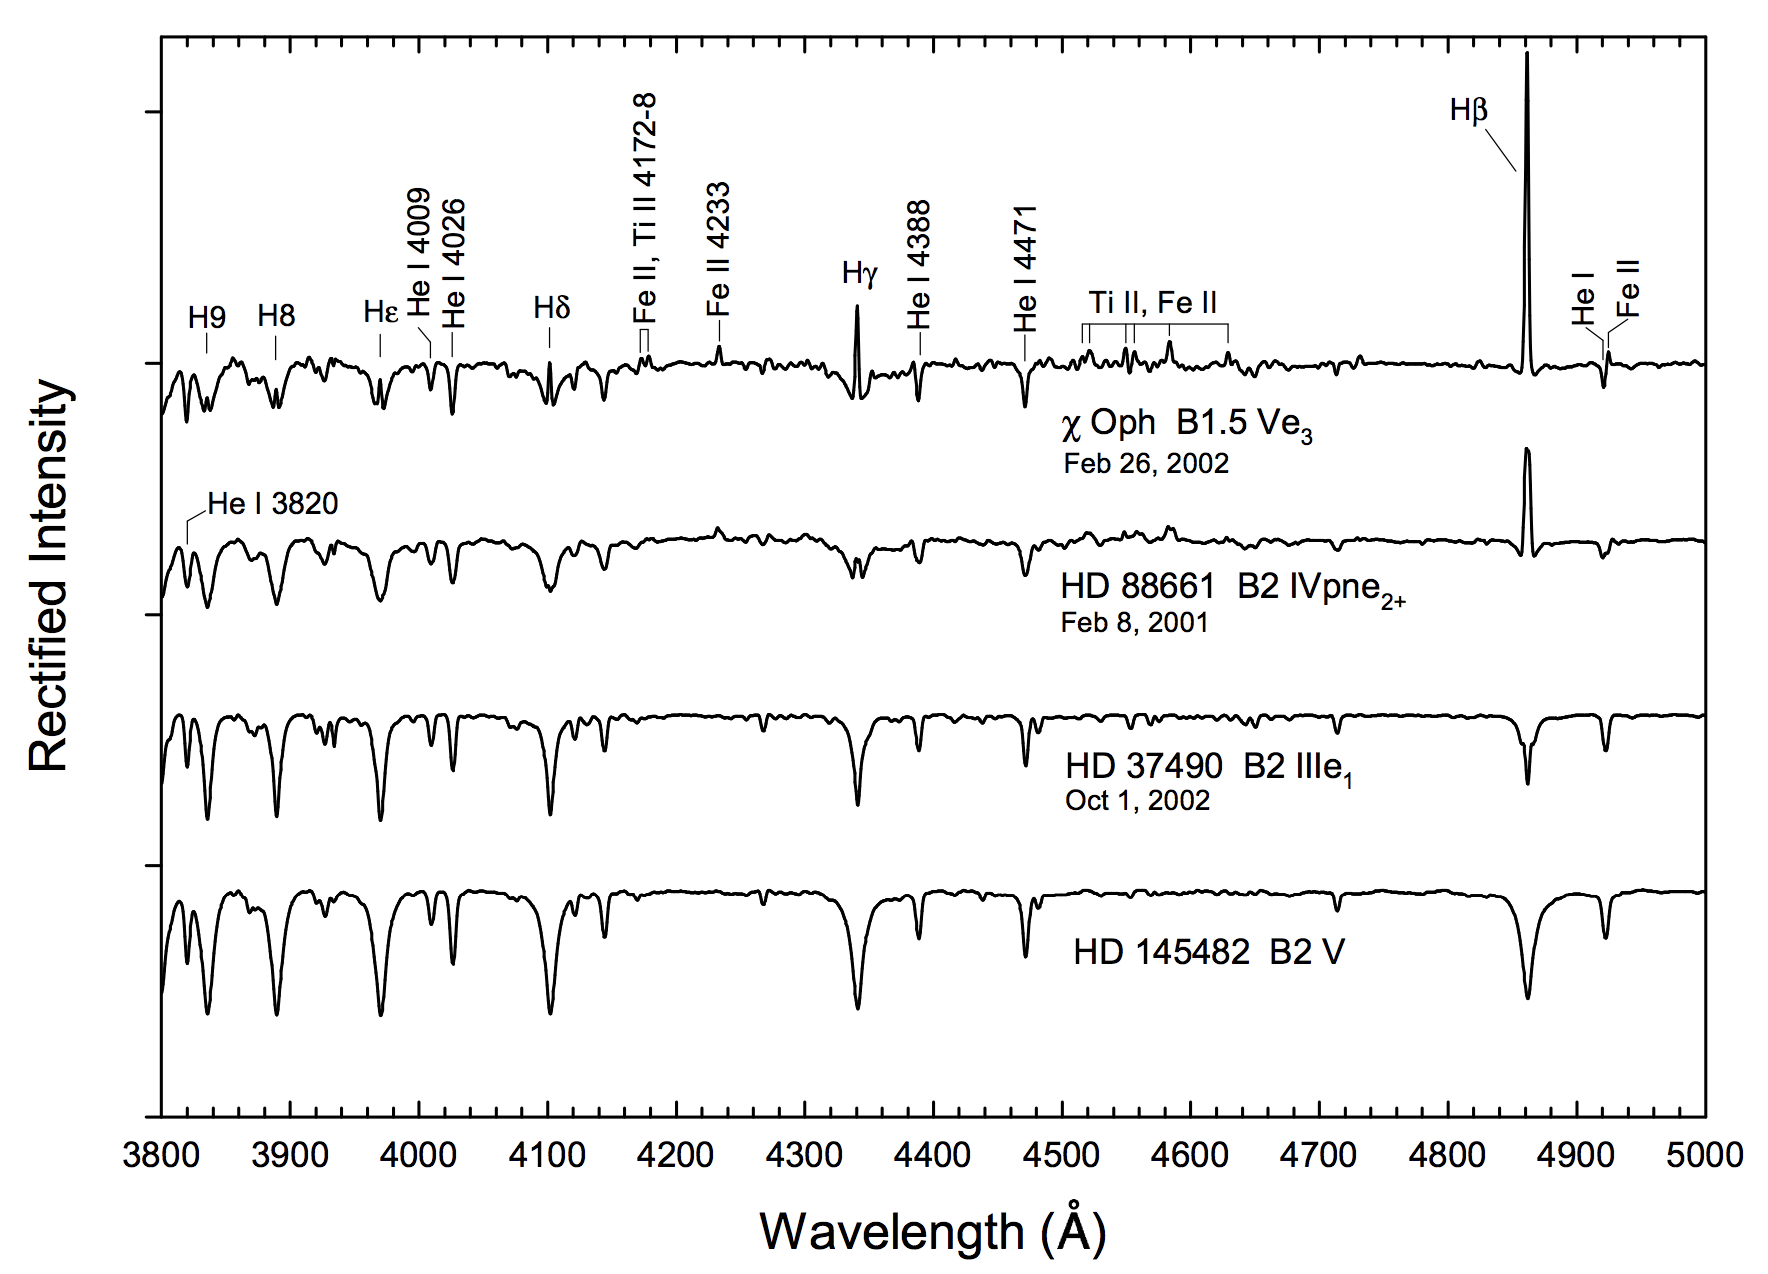
\includegraphics[width=14cm]{figures/Be.png}
    \caption{\footnotesize{A selection of Be stars compared with a B2V secondary standard, HD 145482. The spectral types are on the Lesh (1968) system. Spectra from the Paranal Observatory spectral library. Figure taken from Gray (2009).}}
    \label{fig:be}
\end{figure}

{\noindent}Near a spectral type of A0, the primary luminosity criterion is the progressive widening and strengthening of the hydrogen lines with decreasing luminosity. The hydrogen lines reach a maximum in the A-type stars. The CaII K-line increases significantly in strength through the A-type stars, and its absolute strength, or, more usefully, its ratio with H$\epsilon$ or H$\delta$ is a sensitive indicator of the temperature type, although one that is dependent on the metallicity. The general metallic-line spectrum also increases in strength through the A-type stars. These three criteria give a consistent temperature type in the normal A-type stars. Any disagreement between these three criteria indicates the star is peculiar in some way. \textbf{Ap stars} are A-type (actually more commonly late B-type) stars that show significant enhancements of certain elements. \textbf{Herbig Ae stars} generally show emission in the H$\alpha$ line (outside of the spectral range of most of the spectra used in this atlas), and quite often emission in H$\beta$ and even H$\gamma$. Many Herbig Ae stars are still contracting to the main sequence, and are thus either still surrounded by remnants of their stellar cocoons, or have developed massive stellar winds.

{\noindent}Metallic-line A-type stars, or, for short, \textbf{Am stars}, are defined as stars that show a difference between the K-line type and the metallic-line type. Many Am stars show the \textbf{anomalous luminosity effect} in which the luminosity criteria in certain spectral regions (in particular, the region from $4077$\AA$-4200$\AA) may indicate a giant or even a supergiant luminosity, whereas other regions indicate a dwarf luminosity or even lower.

{\noindent}The hydrogen lines continue to weaken through the F-type stars, and the CaII K-line strengthens, although it becomes essentially saturated by the late F-type stars. The general strength of the metallic-line spectrum grows dramatically. Around F2, depending upon the resolution of the spectrum, the G-band makes its first appearance. The G-band is a molecular band, composed of thousands of closely spaced lines due to the diatomic molecule CH. By F0, the hydrogen lines have lost most of their sensitivity to luminosity. Note, however, that they can still be used to distinguish the supergiant classes from lower luminosities. Near F0, the luminosity class is estimated from the strength of lines due to ionized iron and titanium. By F8, the hydrogen lines have lost all sensitivity to luminosity, and it is now necessary to rely solely on lines and blends of ionized species.

{\noindent}Later than G0 along the main sequence, the hydrogen lines continue to fade, while the strength of the general metallic-line spectrum continues to increase. The G-band also increases in strength until the early K-type stars (about K3), and then begins to fade.

{\noindent}Molecular features first appear in the spectra of F-type main sequence stars and grow to dominate the spectra of the late-type stars, especially those of types K and M. The main sequence does not end at M4.5, but continues through the late M-, the L- and the T-type dwarfs, a sequence that spans the transition from hydrogen-burning dwarf stars to brown dwarfs. Visible in a number of stars is a broad, shallow depression, centered near $4430$\AA. This is an example of a diffuse interstellar band, probably due to molecules in the
ISM between us and the star. A number of G and K-type giants show either strong or weak molecular bands involving
carbon.

{\noindent}Almost all barium-rich stars are members of binary systems in which the companion is a white dwarf. It is believed that the enhanced abundances of s-process elements, such as barium, were gained from the companion star when it was on the AGB. The mass transfer came about either through \textbf{Roche-lobe overflow} or wind accretion. The \textbf{s-process elements} are the result of slow neutron capture, which occurs only at advanced stages of nuclear burning.

{\noindent}Notice that H$\beta$ is in emission in the M4.5 star; many M dwarfs have active chromospheres and exhibit strong flares many times more energetic than solar flares. One of the manifestations of this is emission in the hydrogen lines.

\subsubsection{Follow-up Questions}

\begin{itemize}
    \item Are there emission lines?
    \item What molecular lines are in the Sun?
    \item What important lines are there are much longer wavelengths than those in the optical?
    \item What if the A star had a protoplanetary disk?
    \item What is the significance of a $\lambda$F$_\lambda$ (or $\nu$F$_\nu$) spectrum?
    \item How can the relative height of the stellar vs disk bumps change? (i.e., total energy of the system cannot change; dust bump can't be higher than star bump without extinction.)
\end{itemize}

% --------------------------------------------------------------
%               13. 
% --------------------------------------------------------------

\newpage
\subsection{Question 13}

What can be learned about young stars (T Tauri and pre-main-sequence stars) from an analysis of their spectral features?

\subsubsection{Short answer}

A range of information can be obtained about T Tauri stars and pre-main-sequence stars using spectral analysis:

\begin{itemize}
    \item chemical composition
    \item velocity structure
    \item information on the existence of inflows and/or outflows
    \item rate of contraction (i.e., SFR)
    \item disk properties
    \item accretion rates
    \item age determination (via Lithium abundance)
    \item evolutionary stage (via spectral index)
\end{itemize}

\subsubsection{Additional context}

Since we think star formation begins with a core that is purely gas, we expect to begin with a cloud that is cold and lacks a central point source. Once a protostar forms, it will begin gradually heating up the cloud, while the gas in the cloud collapses onto the protostar, reducing the opacity. Eventually enough material accretes from the envelope to render it transparent in the near infrared and eventually the optical, and we begin to be able to see the star directly for the first time. The star is left with an accretion disk, which gradually accretes and is then dispersed. Eventually the star contracts onto the main sequence.

{\noindent}This theoretical cartoon has been formalized into a system of classification of young stars based on observational diagnostics. At one end of this sequence lies purely gaseous sources where there is no evidence at all for the presence of a star, and at the other end lies ordinary main sequence stars. In between, objects are classified based on their emission in the infrared and sub-mm parts of the spectrum. These classifications probably give more of an impression of discrete evolutionary stages than is really warranted, but they nonetheless serve as a useful rough guide to the evolutionary state of a forming star.

{\noindent}Consider a core of mass $\sim M$, seen in dust or molecular line emission. When a star first forms at its center, the star will be very low mass and very low luminosity, and will heat up only the dust nearest to it, and only by a very small amount. Thus the total light output will still be dominated by the thermal emission of the dust at its equilibrium temperature. The spectral energy distribution of the source will therefore look just like that which prevailed before the star formed.

{\noindent}However, there might be other indicators that a star has formed. For example, the density distribution might show a very sharp, unresolved peak. Another sign that a star has formed might be the presence of an outflow, which all protostars seem to generate. Outflows coming from the center of a core can be detected in a few ways. Most directly, one can see bipolar, high velocity structures in molecular emission (Figure \ref{fig:outflows}).

\begin{figure}[h]
    \floatbox[{\capbeside\thisfloatsetup{capbesideposition={right,top},capbesidewidth=4cm}}]{figure}[\FBwidth]
    {\caption{\footnotesize{\\An integrated intensity map in CO($2\rightarrow1$), showing material at velocities between $\pm30-50\,{\rm km\,s^{-1}}$ (blue and red contours, respectively) relative to the mean (Tafalla et al., 2004). Contours are spaced at intensities of $1\,K\,km\,s^{-1}$. The outflow shown is in the Taurus star-forming region. Figure taken from Krumholtz (2015).}}
    \label{fig:outflows}}
    {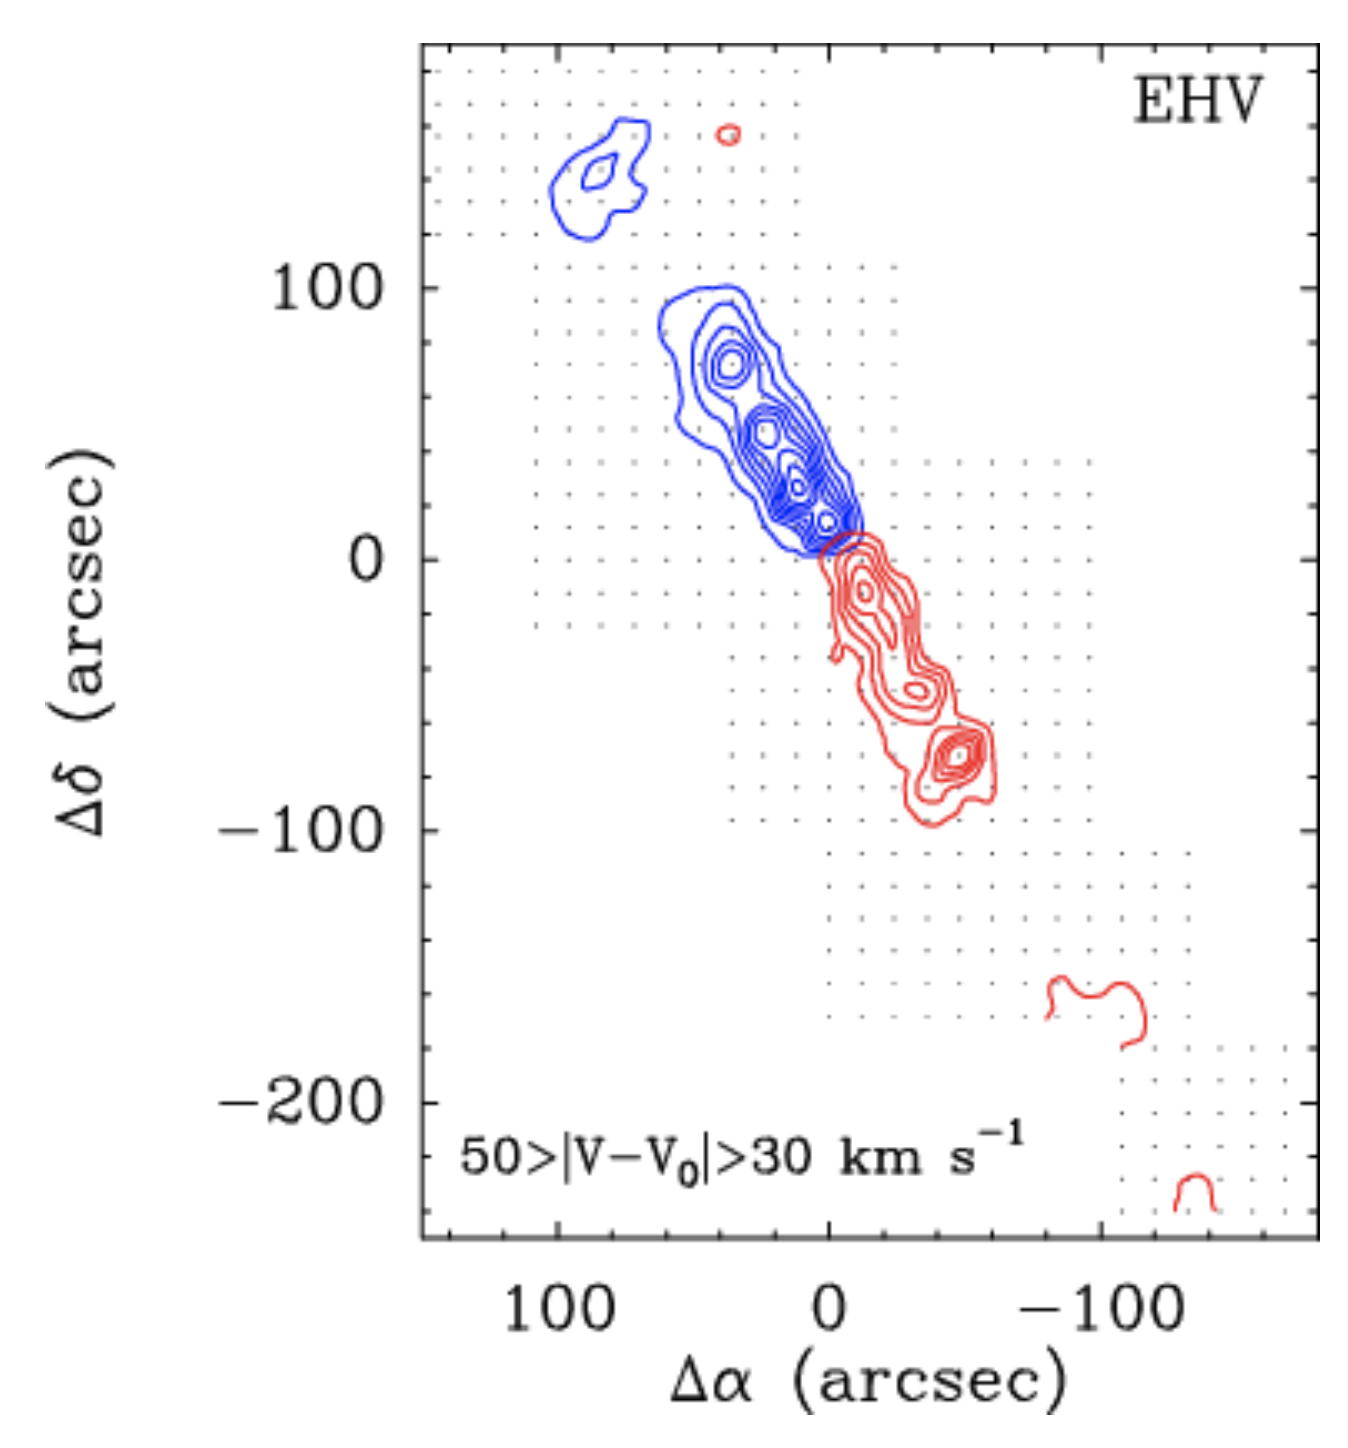
\includegraphics[width=8cm]{figures/Outflows.png}}
\end{figure}

{\noindent}One can also detect indirect evidence of an \textbf{outflow}, from the presence of highly excited molecular line emission that is produced by shocks at hundreds of ${\rm km\,s^{-1}}$. One example of such a line is SiO($2\rightarrow1$) line, which is generally seen in gas moving at several tens of ${\rm km\,s^{-1}}$ with temperatures of several hundred ${\rm K}$ -- this is taken to be indication that emission in this line is produced in warm shocks. Since we know of no processes other than formation of a compact object with a $\gtrsim100\,{\rm km\,s^{-1}}$ escape velocity that can accelerate gas in molecular clouds to such speeds, the presence of such an outflow is taken to indicate that a compact object has formed.

{\noindent}These are the earliest indications of star formation we have available to us. We call objects that show one of these signs, and do not fall into one of the other categories, \textbf{class 0 sources}. The dividing line between class 0 and class 1 is that the star begins to produce enough heating that there is non-trivial infrared emission. Before the advent of Spitzer and Herschel, the dividing line between class 0 and 1 was taken to be a non-detection in the IR, but as more sensitive IR telescopes became available, the detection limit went down of course. Today, the dividing line is taken to be a luminosity cut. A source is said to be class 0 if more than 0.5\% of its total bolometric output emerges at wavelengths longer than $350\,\mu{\rm m}$, i.e., if $L_{\rm smm}/L_{\rm bol}>0.5\%$, where $L_{\rm smm}$ is defined as the luminosity considering only wavelengths of $350\,\mu{\rm m}$ and longer (see Figure \ref{fig:protostellarseds}).

\begin{figure}[t!]
    \centering
    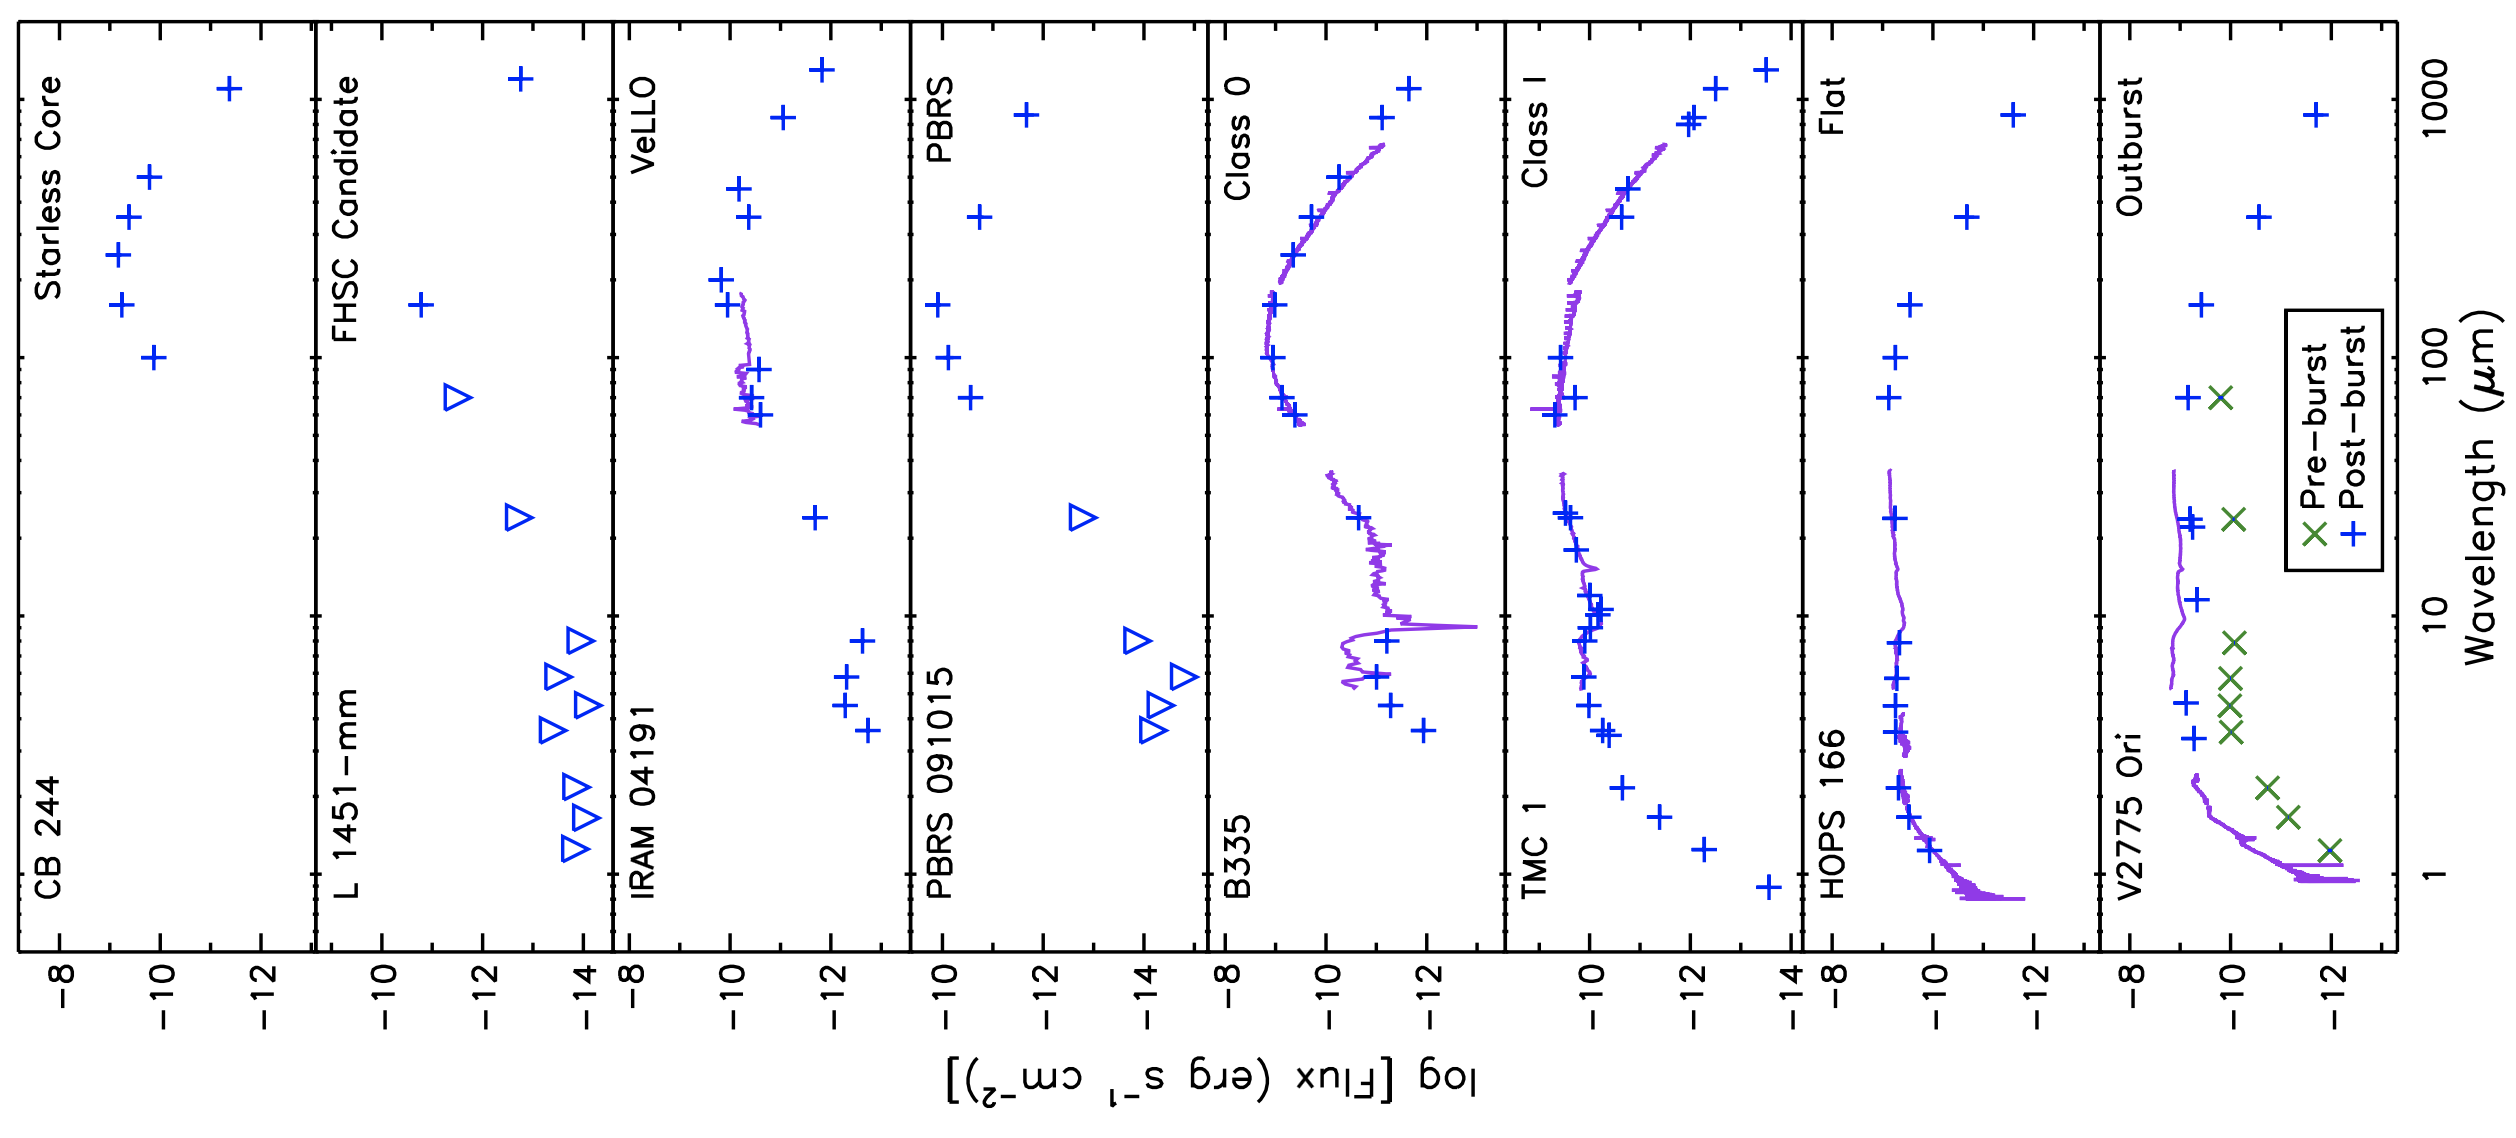
\includegraphics[width=10.5cm]{figures/ProtostellarSEDs.png}
    \caption{\footnotesize{Sample SEDs of protostellar cores, together with the assigned class, as collected by Dunham et al. (2014). Figure taken from Krumholtz (2015).}}
    \label{fig:protostellarseds}
\end{figure}

{\noindent}In practice, measuring $L_{\rm smm}$ can be tricky because it can be hard to get absolute luminosities (as opposed to relative ones) correct in the sub-mm, so it is also common to define the class $0-1$ divide in terms of another quantity: the bolometric temperature $T_{\rm bol}$. This is defined as the temperature of a blackbody that has the same flux-weighted mean frequency as the observed SED. That is, if $F_\nu$ is the flux as a function of frequency from the observed source, then we define $T_{\rm bol}$ by the implicit equation 

\begin{align*}
    \frac{\int\nu F_\nu {\rm d}\nu}{\int F_\nu {\rm d}\nu} = \frac{\int\nu B_\nu(T_{\rm bol}){\rm d}\nu}{\int B_\nu(T_{\rm bol}){\rm d}\nu}.
\end{align*}

{\noindent}The class $0-1$ dividing line is also sometimes taken to be $T_{\rm bol}=70\,{\rm K}$. In cases where $L_{\rm smm}$ is accurately measured, $T_{\rm bol}$ is observed to be a reasonably good proxy for $L_{\rm smm}/L_{\rm bol}$.

{\noindent}Once protostars reach \textbf{class I}, their evolution into further classes is defined in terms of the infrared SED. The motivating cartoon is a follows. At early times, the envelope of dust around the protostar is very optically thick at visible and even near infrared wavelengths. As a result, we don't get to see the stellar photosphere at all. All the radiation is absorbed by the envelope. The dust is in thermal equilibrium, so it re-radiates that energy. Since the radius of the sphere of dust is much larger than that of the star, and the luminosity radiated by the dust must ultimately be equal to that of the star, this emission must be at lower temperature and thus longer wavelengths. Thus as the radiation propagates outward through the dust it is shifted to longer and longer wavelengths. However, dust opacity decreases with wavelength, and thus eventually the radiation is shifted to wavelengths where the remaining dust is optically thin, and it escapes. What we observe is therefore not a stellar photosphere, but a ``dust photosphere''.

{\noindent}Given this picture, the greater the column density of the dust around the star, the further it will have to diffuse in wavelength in order to escape. Thus the wavelength at which the emission peaks, or, roughly equivalently, the slope of the spectrum at a fixed wavelength, is a good diagnostic for the amount of circumstellar dust. Objects whose SEDs peak closer to the visible are presumed to be more evolved, because they have lost most of their envelopes.

{\noindent}More formally, this classification scheme was based on fluxes as measured by the IRAS satellite. We define

\begin{align*}
    \alpha_{\rm IR} = \frac{{\rm d}\log\lambda F_\lambda}{{\rm d}\log \lambda} ~ [{\rm dimensionless}],
\end{align*}

{\noindent}as the \textbf{IR spectral index}. In practice we measure $\alpha_{\rm IR}$ using two points from the IRAS SED: $2.2\,\mu{\rm m}$ and $10-25\,\mu{\rm m}$. More positive values of $\alpha_{\rm IR}$ indicate SEDs that peak at longer wavelengths, further into the IR, while more negative values indicate SEDs that peak closer to visible. We define sources with $\alpha_{\rm IR}\geq0.0$ (i.e., rising at longer wavelengths from $2-25\,\mu{\rm m}$, as class I sources. Alternately, in terms of bolometric temperature, the class I to class II transition is generally taken to be at 650 K.

{\noindent}As more of the envelope accretes, it eventually becomes optically thin at the peak emitting wavelengths of the stellar photosphere. In this case we see the stellar blackbody spectrum, but there is also \textbf{excess infrared emission} coming from the disk of warm, dusty gas that till surrounds the star. Thus the SED looks like a stellar blackbody plus some extra emission at near- or mid-IR wavelengths. Stars in this class are also know as \textbf{classical T Tauri stars}, named for the first object of the class, although the observational definition of a T Tauri star is somewhat different than the IR classification scheme, so the alignment may not be perfect.

{\noindent}In terms of $\alpha_{\rm IR}$, these stars have indices in the range  $-1.6<\alpha_{\rm IR}<0$. (Depending on the author, the break-point may be placed at $-1.5$ instead of $-1.6$. Some authors also introduce an intermediate classification between 0 and I, which they take to be $-0.3<\alpha_{\rm IR}<0.3$.) A slope of around $-1.6$ is what we expect for a bare stellar photosphere without any excess infrared emission coming from circumstellar material. Since the class II phase is the last one during which there is a disk of any significant mass, this is also presumably the phase where planet formation must occur.

{\noindent}The final class is \textbf{class III}, which in terms of SED have $\alpha_{\rm IR}<-1.6$. Stars in this class correspond to \textbf{weak line T Tauri stars}. The SEDs of these stars look like bare stellar photospheres in the optical through the mid-infrared. If there is any IR excess at all, it is in the very far IR, indicating that the emitting circumstellar material is cool and located far from the star. The idea here is that the disk around them has begun to dissipate, and is either now optically thin at IR wavelengths or completely dissipated, so there is no strong IR excess.

{\noindent}However, these stars are still not mature MS stars. First of all, their temperatures and luminosities do not correspond to those of MS stars. Instead, they are still puffed up to larger radii, so they tend to have either lower effective temperatures or higher bolometric luminosities (or both) than MS stars of the same mass. Second, they show extremely high levels of magnetic activity compared to MS stars, producing high levels of x-ray emission. Third, they show lithium absorption lines in their atmospheres. This is significant because lithium is easily destroyed by nuclear reactions at high temperatures, and no main sequence stars with convective photospheres show Li absorption. Young stars show it only because there has not yet been time for all the Li to burn.

To summarize,

\begin{itemize}
    \item \textbf{Class 0} protostars are objects that are so heavily obscured that their spectra peak at $\lambda>100\,\mu{\rm m}$. For these sources, $\alpha_{\rm IR}$ is not a useful characteristic, because the source may be invisible at $2.2\,\mu{\rm m}$, and at $10\,\mu{\rm m}$ there may be deep absorption by cold foreground silicate dust. Inward motions of the gas are sometimes revealed by asymmetric profiles of molecular emission lines. The lifetime of a Class 0 object is short, $\sim1-3\times10^4\,{\rm yr}$.
    \item \textbf{Class I} protostars have $\alpha_{\rm IR}>0$: there is more power being radiated near $10\,\mu{\rm m}$ than near $2\,\mu{\rm m}$. Blackbodies with $T<870\,{\rm K}$ have $\alpha_{\rm IR}>0$. Class I protostars are thought to have typical ages $\sim1-2\times10^5\,{\rm yr}$.
    \item \textbf{Class II} YSOs have $-1.5<\alpha_{\rm IR}<0$. Blackbodies with $870<T<1540\,{\rm K}$ have such IR spectral indices. Class II YSOs correspond to classical T Tauri stars, which are pre-main-sequence stars, still undergoing gravitational contraction, with substantial accretion disks and accretion rates $\sim10^{-6}\,{\rm M_\odot\,yr^{-1}}$.
    \item \textbf{Class III} protostars have $\alpha_{\rm IR}<-1.6$. Blackbodies with $T>1540\,{\rm K}$ have such spectral indices. Class III YSOs correspond to \textbf{weak-lined T Tauri stars}, which are pre-main-sequence stars still undergoing gravitational contraction, but where the accretion disk is either weak or perhaps entirely absent.
\end{itemize}

{\noindent}The observed flux ratios are determined by the temperature of the emitting regions (star and inner disk) and by wavelength-dependent extinction. Classification of a given object as either Class I or Class II may depend on the source orientation. If we are viewing the object face-on it, may be classified as Class II, but an identical disk viewed edge-on could heavily redden the light reaching the observer, so that the object could be classified as Class I or even Class 0.

{\noindent}\textbf{Infall signatures}: The H$\alpha$ is particularly interesting, because it tells us something about the star's immediate environment. For MS stars, the H$\alpha$ line profile is a result of absorption at the stellar photosphere and emission from the chromosphere. At the photosphere there is a population of neutral hydrogen atoms in the $n=2$ level that absorbs photons at H$\alpha$ frequencies, producing absorption. Above that in the chromosphere is an optically thin, hot gas, which contains atoms in the $n=3$ level. Some of these emit H$\alpha$ photons, partially filling in the absorption trough, but leaving the line overall in absorption. 

{\noindent}Producing Ha in emission is tricky, however. The emitting material must be above the stellar photosphere, so it can fill in the absorption trough created there. This gas must be at temperatures of $5,000-10,000\,{\rm K}$ to significantly populate the $n=3$ level. However, in order to produce enough H$\alpha$ photons to fill in the trough and produce net emission, this gas must also be dense enough for the collision rate to be high enough to force the $n=3$ level close to LTE. 

\begin{figure}[t!]
    \centering
    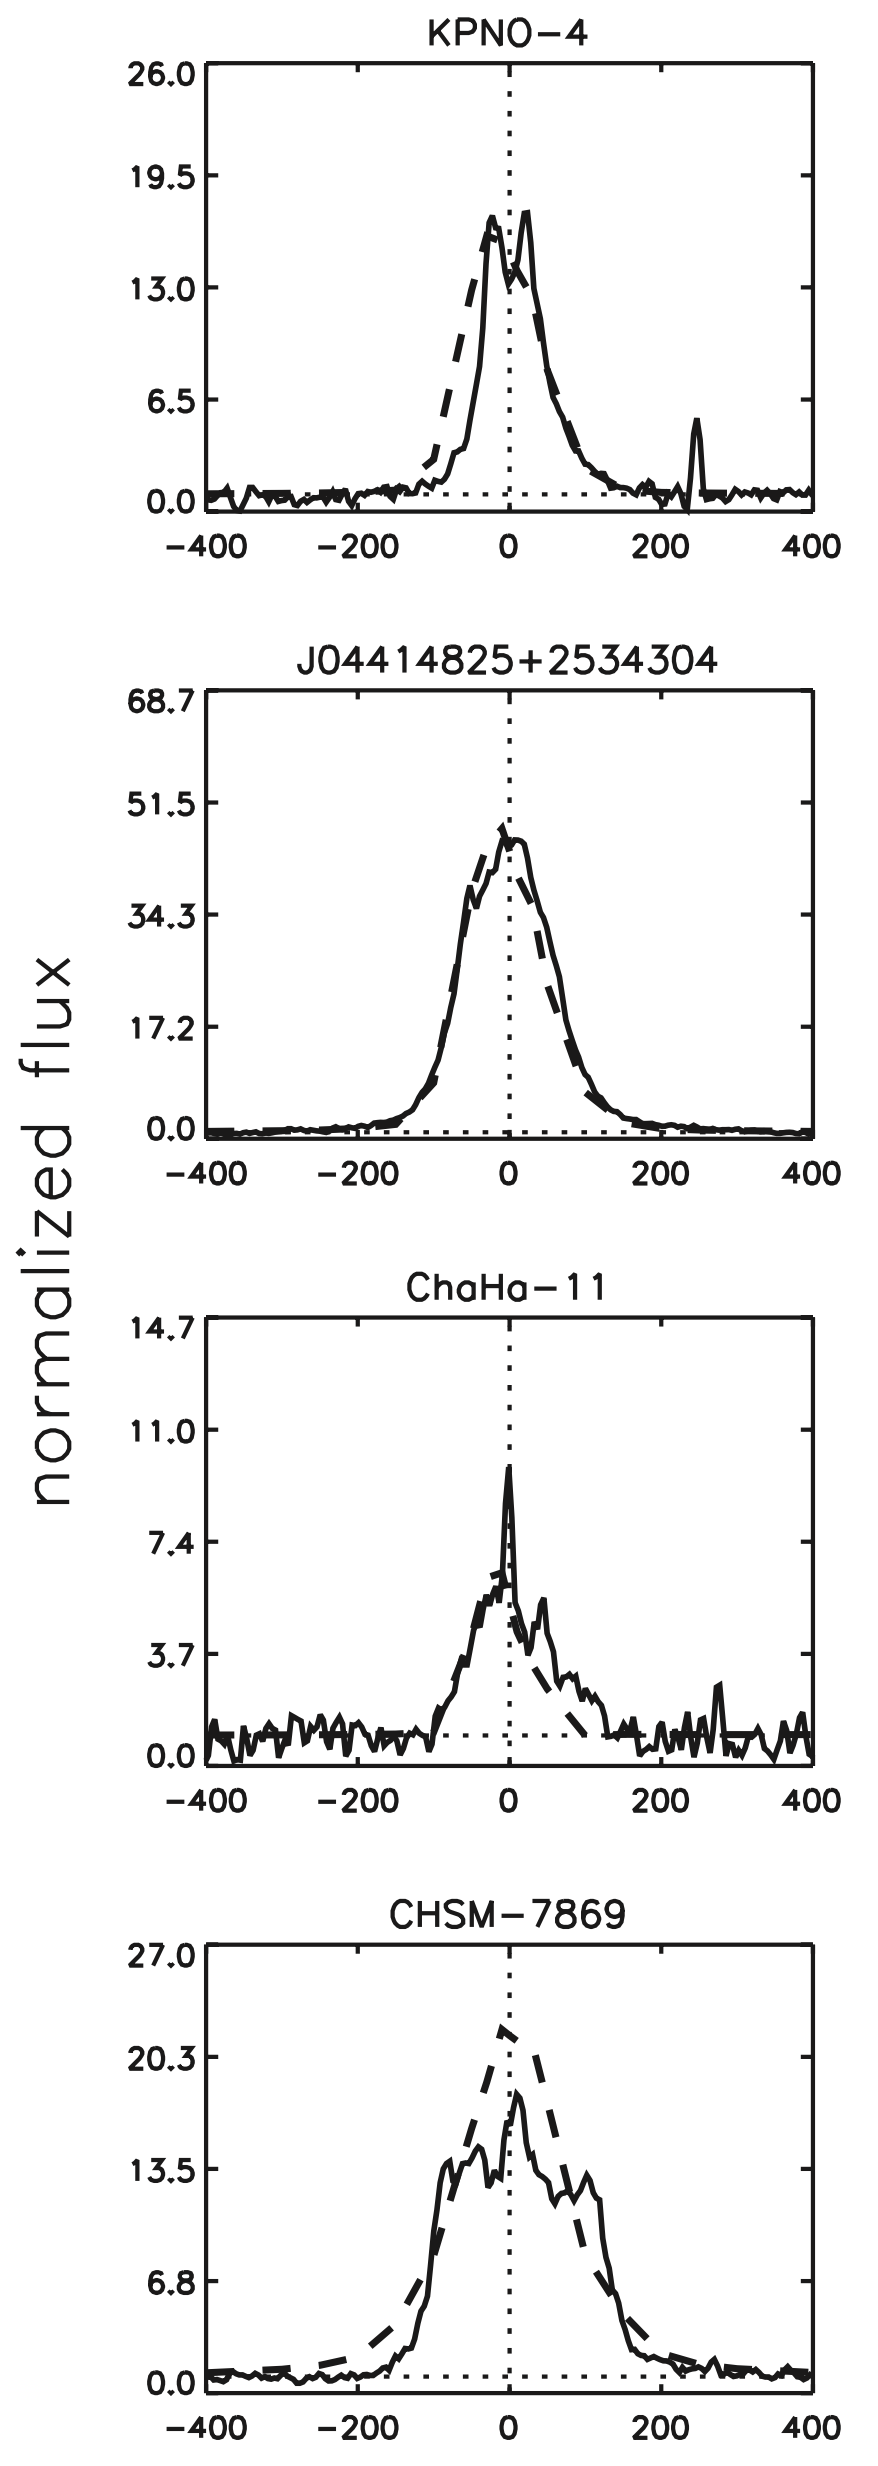
\includegraphics[width=8.25cm]{figures/TTinfall.png}
    \caption{\footnotesize{Comparisons between observed (solid) and model (dashed) H$\alpha$ line profiles for a sample of T Tauri stars (Muzerolle et al., 2005). The $x$ axis shows velocity in ${\rm km\,s^{-1}}$. Each model curve is a fit in which the accretion rate is one of the free parameters. Figure taken from Krumholtz (2015).}}
    \label{fig:ttinfall}
\end{figure}

{\noindent}Ordinary stellar chromospheres have densities that are much too low to meet this requirement. This H$\alpha$ emission implies the presence of material around the star at temperatures of $5,000-10,000\,{\rm K}$, but at densities much higher than found in an ordinary stellar chromosphere. Moreover, the width of the $H\alpha$ emission requires that this material be moving at velocities of hundreds of ${\rm km\,s^{-1}}$ relative to the stellar surface (i.e., comparable to the free-fall velocity). This cannot be thermal broadening, because this would require temperatures of $\sim10^6\,{\rm K}$ high enough to completely ionize hydrogen. It muse therefore be bulk motion.

{\noindent}The standard inference is that this indicates the presence of gas infalling onto the stellar surface. Such gas would provide the high densities required to produce Ha in emission. The infall of this material would provide the requisite bulk motion. Internal shocks and the shocking of this gas against the stellar surface could easily heat gas to the required temperatures. Finally, this hot material would also produce continuum emission, explaining the continuum veiling.

{\noindent}Quantitative radiative transfer calculations that attempt to fit the observed veiling and line emission can be used to infer the densities and velocities of the circumstellar gas, thereby constraining the accretion rate (Figure \ref{fig:ttinfall}). The inferred accretion rates depend on the strength of the H$\alpha$ emission, and are typically $10^8\,{\rm My\,yr^{-1}}$. There is a broad range, however, running from $10^{-11}-10^{-6}\,{\rm M\,yr^{-1}}$, with a very rough correlation $\dot{M}_*\propto M_*^2$.

{\noindent}These accretion rates are generally low enough so that accretion luminosity does not dominate over stellar surface emission. However, the estimated accretion rates are extremely uncertain, and the models used to make these estimates are very primitive. In general they simply assume that a uniform density slab of material arrives at the free-fall velocity, and covers some fraction of the stellar surface, and the accretion rate is inferred by determining the density of this material required to produce the observed spectral characteristics.

{\noindent}Despite this caveat, though, the H$\alpha$ line and other optical properties do seem to indicate that there must be some dense infalling material even around these stars that lack obvious envelopes. This in turn requires a reservoir of circumstellar material not in the form of an envelope, which is most naturally provided by a disk. Indeed, before the advent of space-based IR observatories, optical indicators like this were the only real evidence we had for disks around T Tauri and Herbig Ae/Be stars.

{\noindent}\textbf{Disk lifetimes}: We now turn to the disks that surround T Tauri and similar stars. Prior to the 2000s, we had very little direct information about such objects, since they are not visible in the optical. That changed dramatically with the launch of space-based IR observatories, and the developed of ground-based millimeter interferometers. These new techniques made it possible to observe disks directly for the first time.

{\noindent}One of the most interesting properties of disks for those who are interested in planets is their lifetimes. This sets the limit on how long planets have to form in a disk before it is dispersed. In discussing disk lifetimes, it is important to be clear on how the presence or absence of a disk is to be inferred, since different techniques probe different parts and types of disks. In general what all these techniques have in common is that one uses some technique to survey young star clusters for disks. The clusters can be age-dated using pre-main sequence or main sequence HR diagrams. One then plots the disk fraction against age.

{\noindent}One signature of disks we have already discussed: optical line emission associated with accretion in T Tauri stars, particularly H$\alpha$. Surveys of nearby groups find that H$\alpha$ line emission usually disappears at times between $1$ and $10\,{\rm Myr}$ (Figure 19.4). This tells us that the inner parts of disks ($\lesssim1\,{\rm AU}$) which feed stars disappear over this time scale. In contrast, ground-based near IR observations tell us about somewhat more distant parts of the disk, out to a few ${\rm AU}$. The timescales implied by these results are very similar those obtained from the H$\alpha$: roughly half the systems lose their disks within $\sim3\,{\rm Myr}$.

\begin{figure}[t]
    \centering
    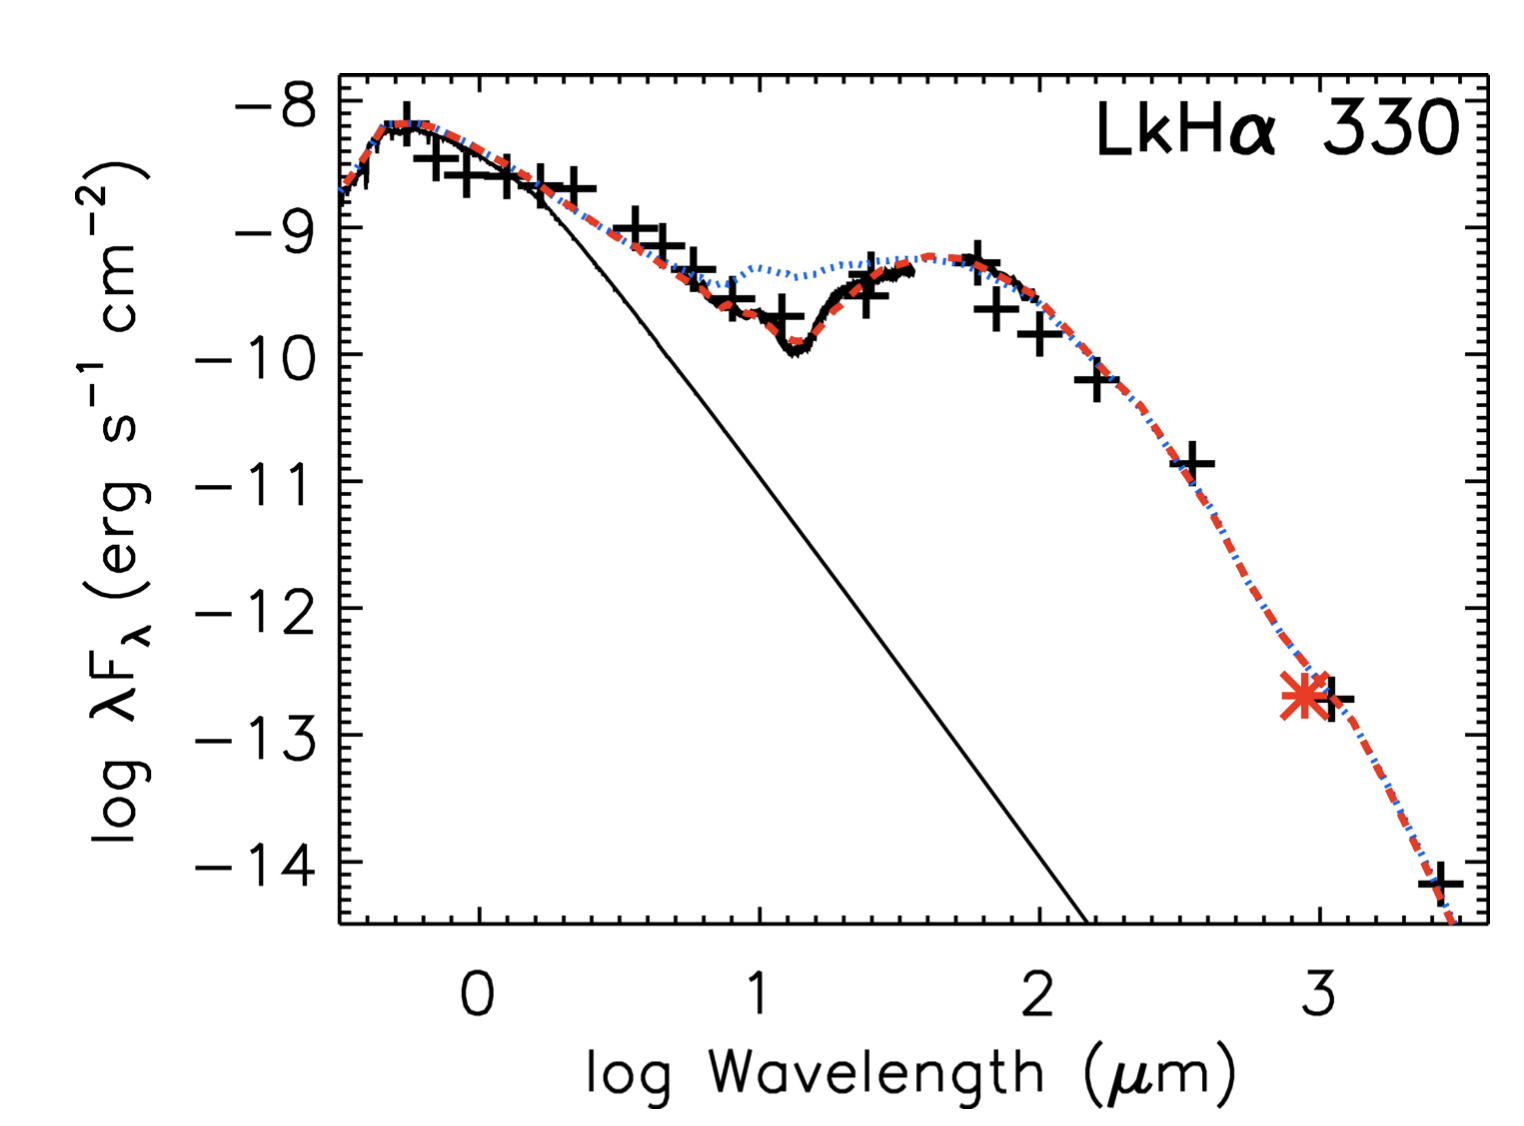
\includegraphics[width=7.5cm]{figures/LkHa330.png}
    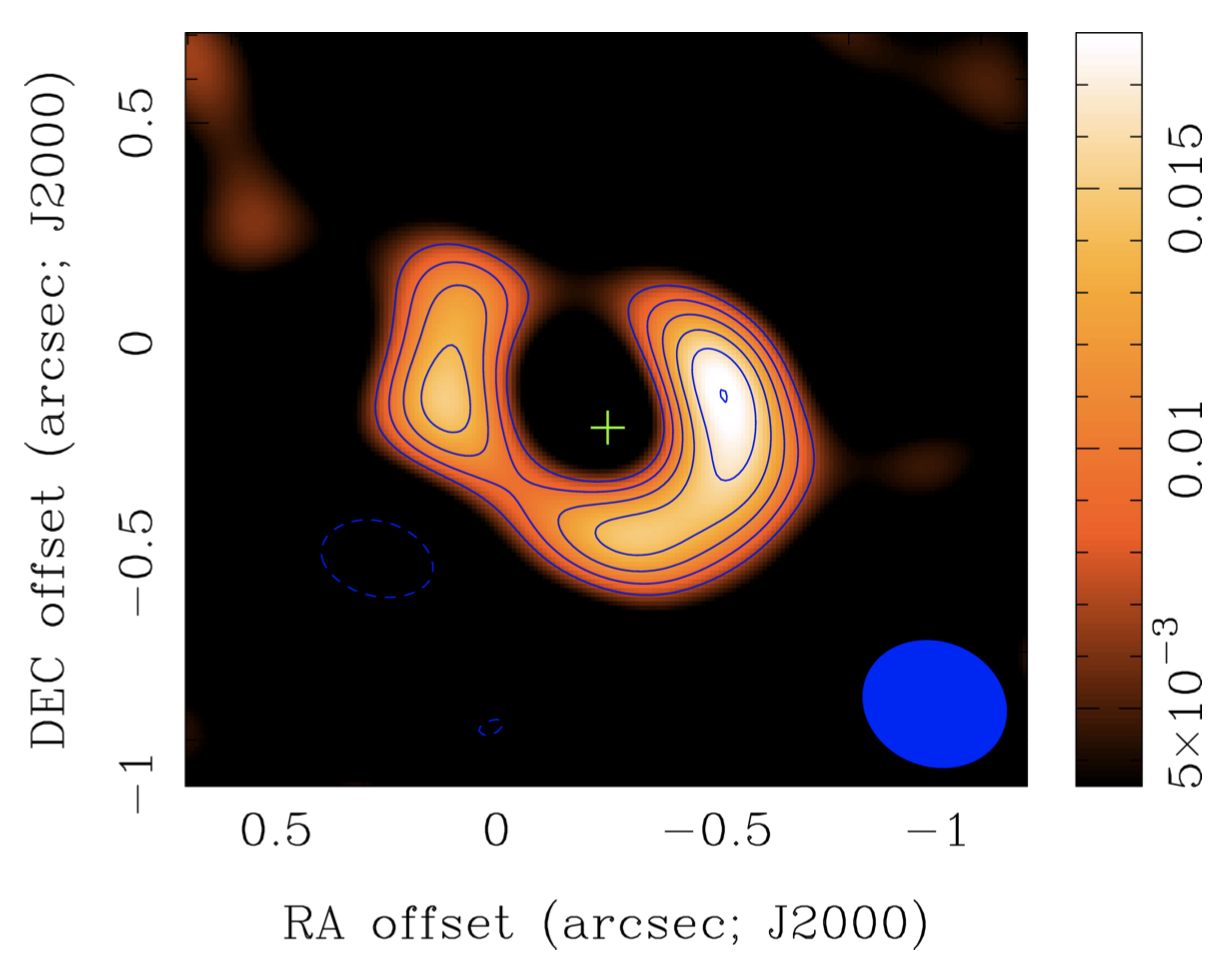
\includegraphics[width=7.5cm]{figures/LkHa330_cont.png}
    \caption{\footnotesize{(\textbf{Left:}) The SED of the star ${\rm LkH}\alpha\,330$ (Brown et al., 2008). Plus signs indicate measurements. The black line is a model for a stellar photosphere. The blue line is a model for a star with a disk going all the way to the central star, while the red line is a model for disk with a $40\,{\rm AU}$ hole in its center. Figure taken from Krumholtz (2015). (\textbf{Right:}) Dust continuum image of the disk around ${\rm LkH}\alpha\,330$, taken at $340\,{\rm GHz}$ by the SMA (Brown et al., 2008). Colors show the detected signal, and contours show the signal to noise ratio, starting from S/N of $3$ and increasing by $1$ thereafter. The green plus marks the location of the star. The blue circle is the SMA beam. Figure taken from Krumholtz (2015).}}
    \label{fig:lkha330}
\end{figure}

{\noindent}These observations are sensitive primarily to the inner disk, and the IR techniques are generally sensitive only in cases where the dust in these regions is optically thick. Some optically thin material could still be present and would not have been detected. Observations at longer wavelengths, such as Spitzer's $24\,\mu{\rm m}$ band and in the ${\rm mm}$ regime from ground-based radio telescopes, probe further out in disks, at distances of $\sim10-100\,{\rm AU}$. They are also sensitive to much lower amounts of material. Interestingly, unlike the shorter wavelength observations, these measurements indicate that a small but non-zero fraction of systems retain some disks out to times of $\sim10^8\,{\rm yr}$. The amounts of mass needed to explain the long wavelength excess are only $\sim10^{-5}\,{\rm M_\odot}$ in dust. Thus the older systems are likely looking at an even later evolutionary phase than T Tauri disks, one in which almost all the gas and inner disk material is gone. These are \textbf{debris disks}, which are thought to originate from collisions between larger bodies than than to be made up of dust from interstellar gas.

{\noindent}\textbf{Transition disks}: The observation that accreting disks and inner optically thick disks disappear on a few ${\rm Myr}$ timescales, but that some fraction leave behind very small amounts of mass in the outer disk is a very interesting one. Observationally, we would like to get some constraints on how the process of a gaseous, accreting T Tauri disk transitioning to a low-mass debris disk occurs. For this purpose, there is an intriguing class of objects known as \textbf{transition disks}. Spectrally, these are defined as objects that have a significant $24\,\mu{\rm m}$ excess (or excess at even longer wavelengths), but little or no IR excess (Figure \ref{fig:lkha330}, left). This SED suggests a natural physical picture: a disk with a hole in its center. The short wavelength emission normally comes from near the star, and the absence of material there produces the lack of short wavelength excess. Indeed, it is possible to fit the SEDs of some stars with models with holes.

{\noindent}In the last decade it has become possible to confirm the presence of inner holes in transition disks directly, at least cases where the inferred hole is sufficiently large (Figure \ref{fig:lkha330}, right). The sizes of the holes inferred by the observations are generally very good matches to the values inferred by modeling the SEDs. The holes are remarkably devoid of dust: upper limits on the masses of small dust grains within the hole are often at the level of $\sim10^{-6}\,{\rm M_\odot}$. The sharp edges of the holes indicate that the effect driving them isn't simply the growth of dust grains to larger sizes, which should produce a more gradual transition. Instead, something else is at work. However, in some transition disks gas is still seen within the gap in molecular line emission, which also suggests that whatever mechanism is removing the dust does not necessarily get rid of all the gas as well.

\subsubsection{Follow-up Questions}

\begin{itemize}
    \item How does the spectrum change as planets start to form?
\end{itemize}

% --------------------------------------------------------------
%               14. 
% --------------------------------------------------------------

\newpage
\subsection{Question 14}

Sketch the spectral energy distribution (SED) of a T Tauri star surrounded by a protoplanetary disk. How would the SED change: (a) if the disk develops a large inner hole, (b) if the dust grains in the disk grow in size by agglomeration (with the same total mass)?

\subsubsection{Short answer}

Figure \ref{fig:ttsed_flat} shows a schematic of what the SED of a T Tauri star surrounded by a protoplanetary disk would look like. It can be seen that the total SED is a composite of the stellar blackbody plus the protoplantary disk component.

\begin{figure}[h]
    \floatbox[{\capbeside\thisfloatsetup{capbesideposition={right,top},capbesidewidth=4cm}}]{figure}[\FBwidth]
    {\caption{\footnotesize{\\SED for the flat blackbody disk, with contributions from star and disk identified. Figure taken from Chiang \& Goldreich (1997).}}
    \label{fig:ttsed_flat}}
    {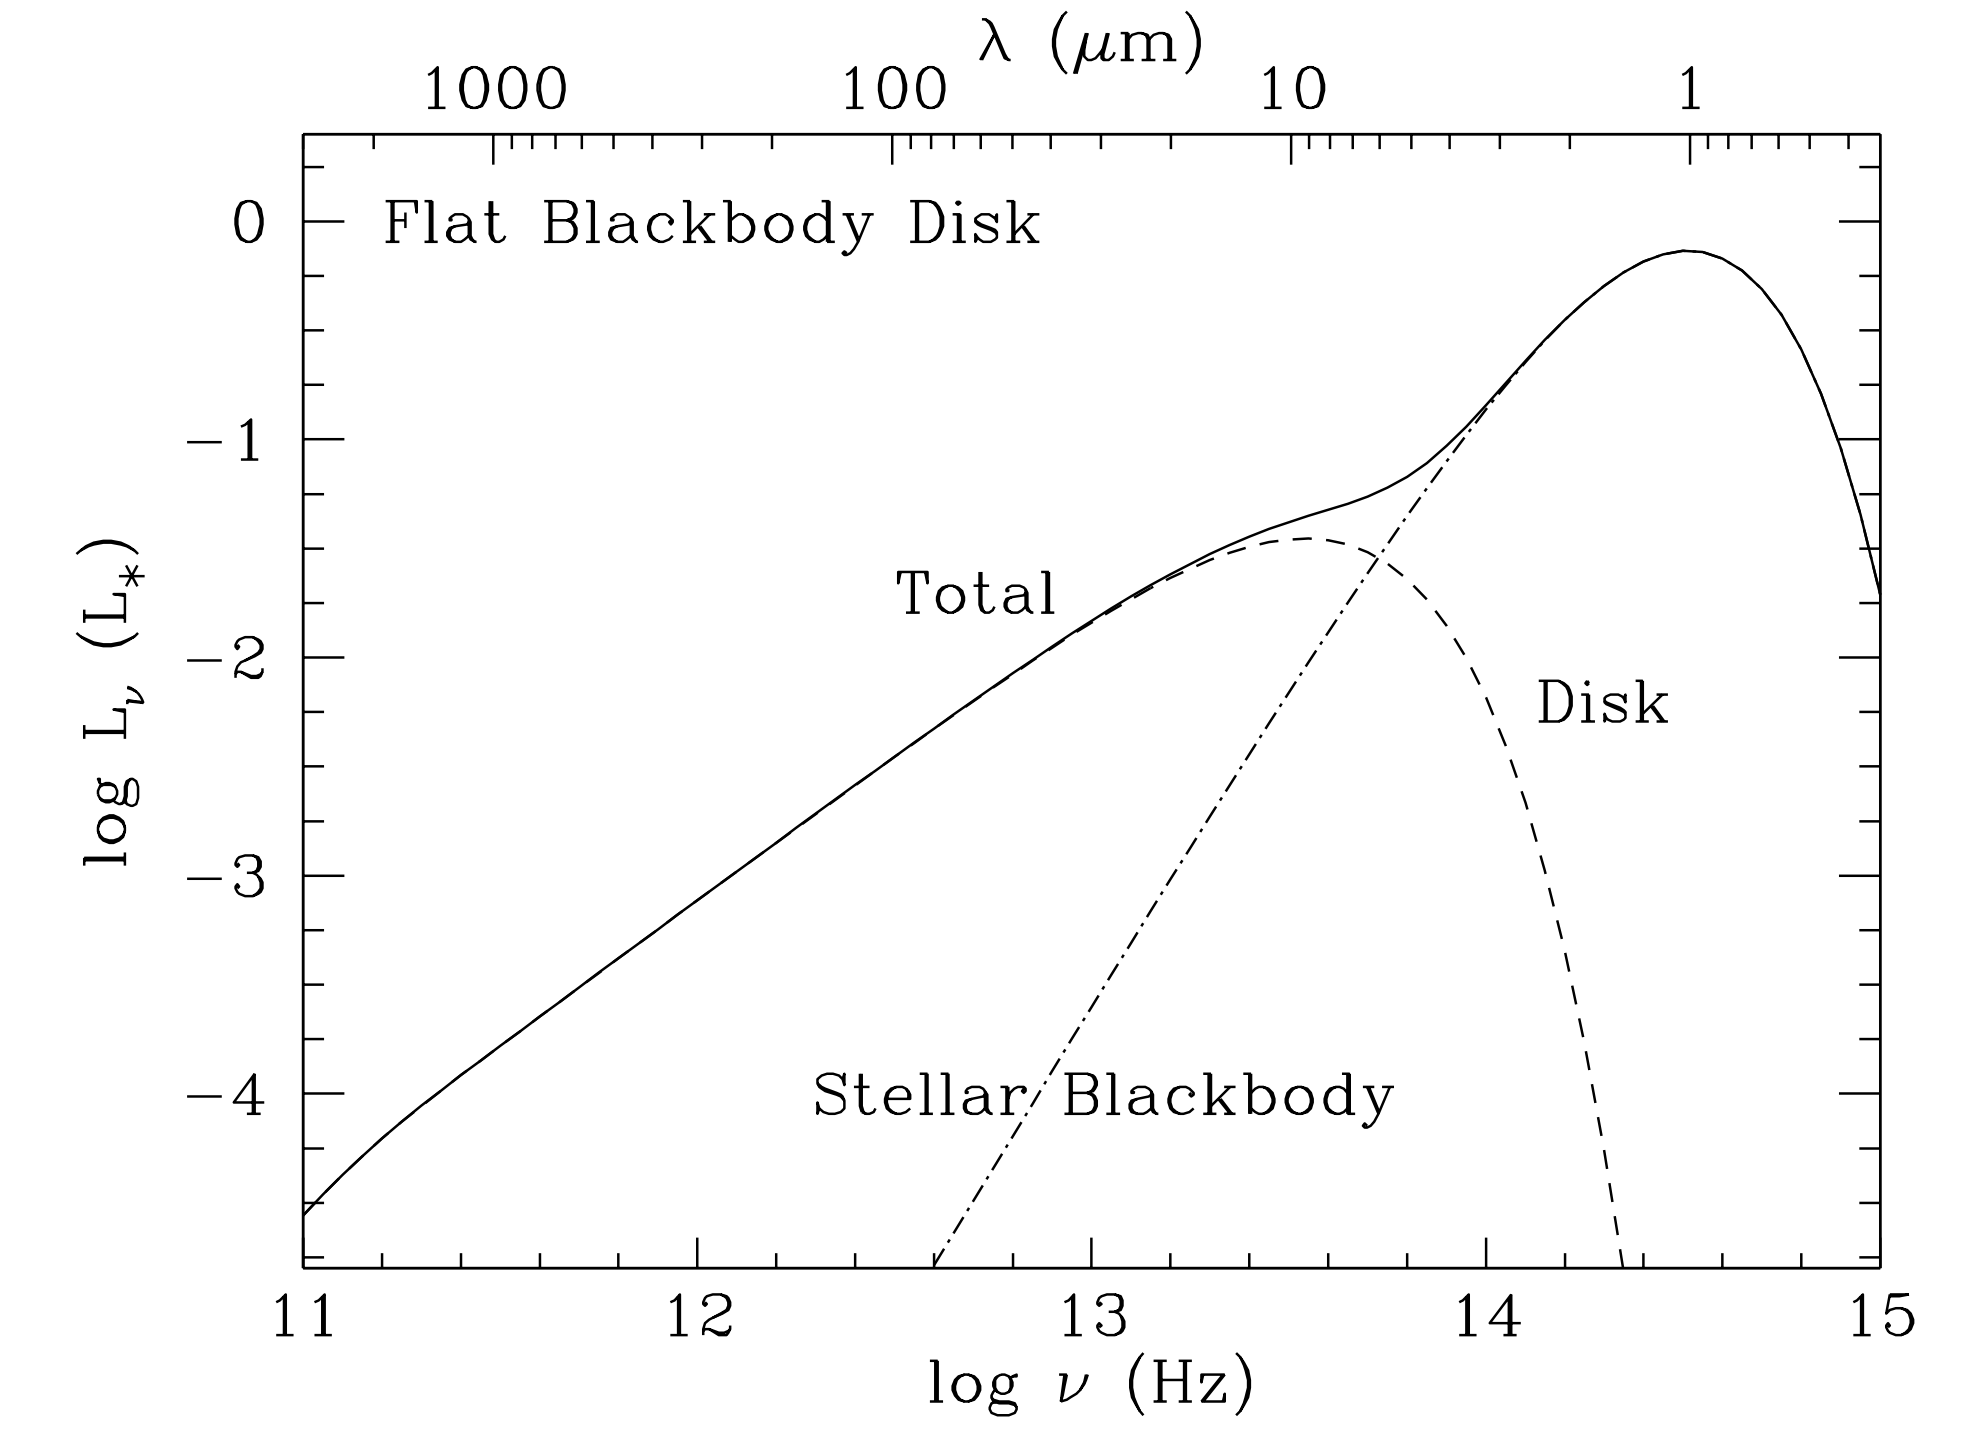
\includegraphics[width=12cm]{figures/TT_SED_flat.png}}
\end{figure}

{\noindent}Figure \ref{fig:lkha330} (left) shows the SED of a T Tauri star surrounded by a protoplanetary disk with a hole in its center. The short wavelength emission normally comes from near the star, and the absence of material there produces the lack of short wavelength excess. Figure \ref{fig:lkha330} (right) shows a continuum image of such a disk.

\begin{figure}[h]
    \centering
    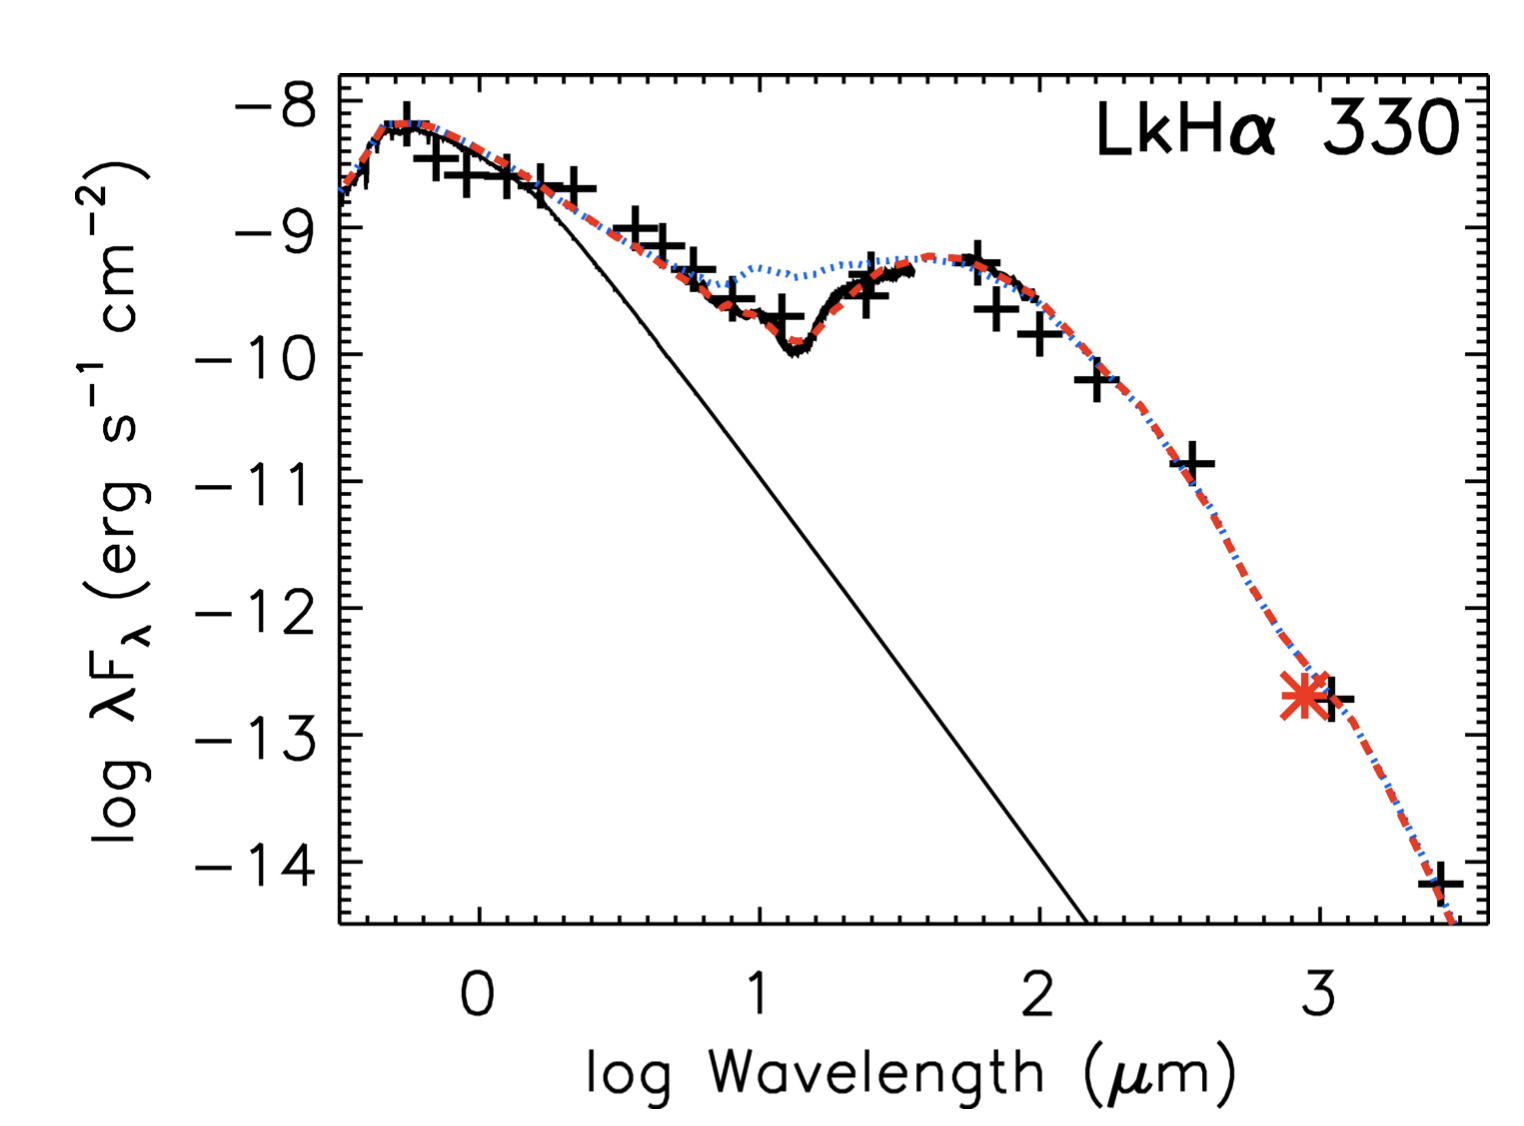
\includegraphics[width=7.5cm]{figures/LkHa330.png}
    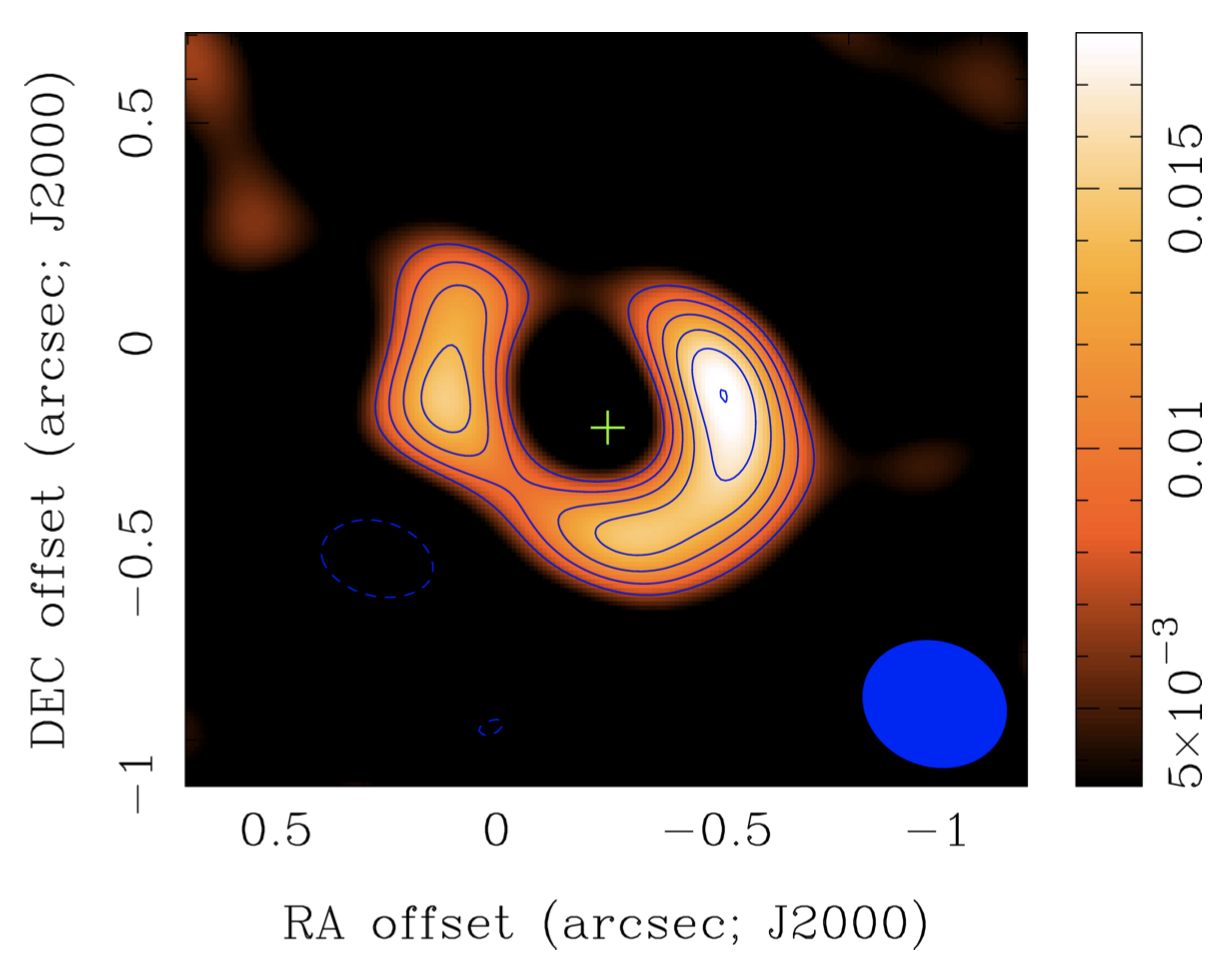
\includegraphics[width=7.5cm]{figures/LkHa330_cont.png}
    \caption{\footnotesize{(\textbf{Left:}) The SED of the star ${\rm LkH}\alpha\,330$ (Brown et al., 2008). Plus signs indicate measurements. The black line is a model for a stellar photosphere. The blue line is a model for a star with a disk going all the way to the central star, while the red line is a model for disk with a $40\,{\rm AU}$ hole in its center. Figure taken from Krumholtz (2015). (\textbf{Right:}) Dust continuum image of the disk around ${\rm LkH}\alpha\,330$, taken at $340\,{\rm GHz}$ by the SMA (Brown et al., 2008). Colors show the detected signal, and contours show the signal to noise ratio, starting from S/N of $3$ and increasing by $1$ thereafter. The green plus marks the location of the star. The blue circle is the SMA beam. Figure taken from Krumholtz (2015).}}
    \label{fig:lkha330}
\end{figure}

\subsubsection{Additional context}

In the pre-main sequence phase, that is, while developing from a voluminous protostar into a star, the accreting stellar objects are powered by gravitational energy, their central temperature still being too low for hydrogen fusion. This situation of stellar evolution is represented by very young protostars ($10^5-10^8\,{\rm yr}$) observed in nebulae where star formation is going on, so-called T Tauri stars (named after their prototype in the constellation of Taurus), which, in many cases, are embedded in protoplanetary nebulae and discs. T-Tauri stars are variable stars; their erratic brightness changes due to instabilities of the accretion disc, violent activity (i.e., stellar winds) in the thin stellar atmosphere (characterized by strong emission lines, mainly H$\alpha$ of the Balmer series, and Ca$^+$), and obscuration by parts of the inhomogeneous surrounding cloud. A very characteristic feature of the T Tauri stars is the higher abundance of lithium relative to the main sequence stars detectable by its $670.7\,{\rm nm}$ line. The lithium isotope $^7$Li is formed in the pp (proton–proton) chain but subsequently eliminated, at temperatures $>2.5\times10^6\,{\rm K}$ by lithium burning during the last highly convective stages when the star enters the MS. The rapid rotation of the T Tauri stars, typically between $1$ and $12$ days, enforces the transport of lithium into the hot stellar core and eventually lithium depletion.

{\noindent}Excess infrared (IR) emission from T Tauri stars is thought to arise from circumstellar disks. The standard disk is modeled as a flat blackbody. In the simplest scenario, it lacks intrinsic luminosity and passively re-radiates the energy it absorbs from the central star. This blackbody model yields an IR spectral energy distribution (SED) of the form $\nu F_\nu\propto\nu^\alpha$, with spectral index $\alpha=4/3$. By coincidence, the steady state accretional luminosity from an opaque, thin disk yields an SED with identical spectral index. SEDs measured between $3$ and $100\,\mu{\rm m}$ are usually well fitted by power laws with $0\leq\alpha\leq4/3$. However, in contrast to the prediction of the standard model, most sources exhibit flattish spectra having $n\leq3/4$. 

{\noindent}The failure of the standard disk model spawned a number of alternative proposals. One of these includes a blackbody disk whose surface flares outward with increasing radius as a consequence of vertical hydrostatic equilibrium. Flared disks intercept more stellar radiation than flat ones, especially at large distances from the star. Other models invoke either an ``active'' disk having a high intrinsic luminosity or a dusty component in addition to the disk.

{\noindent}T Tauri stars have temperatures $T_{\rm TT}\sim4000\,{\rm K}$, masses $M_{\rm TT}\sim0.5\,{\rm M_\odot}$, and radii $R_{\rm TT}\sim2.5\,{\rm R_\odot}$. Dust, which is uniformly mixed with the gas, comprises about $1\%$ of the total mass. Dust grains dominate the continuum opacity from visible through millimeter wavelengths. Dust grains modelled as being spherical have a radius $r\sim0.1\,\mu{\rm m}$, mass density $\rho_d\sim2\,{g\,cm^{-3}}$, and negligible albedo. Their emissivity, which is unity for $\lambda\leq2\pi r$, decreases as $\epsilon_\lambda\sim(2\pi r/\lambda)^\beta$ for $\lambda>2\pi r$. We denote by $\epsilon_\lambda\sim(8\pi rk_BT/hc)^\beta\sim(T/T_{\rm TT})^\beta$ ($\beta\approx1$) the average dust emissivity at temperature $T$. The dust opacity at visual wavelengths is $\kappa_V\sim400\,{\rm cm^2\,g^{-1}}$, which implies an optical depth of $\tau_v\sim4\times10^5a_{\rm AU}^{-3/2}$, where $a_{\rm AU}$ is the disk radius measured in AU.

{\noindent}SEDs are computed for disks viewed pole-on. We choose
an inner cutoff radius, $a_i\sim6R_{\rm TT}\sim0.07\,{\rm AU}$, to mark the condensation boundary of common silicates. The outer cutff radius for flat disks, $a_0\sim2.3\times10^4R_{\rm TT}\sim2.7\times10^2\,{\rm AU}$, is fixed to facilitate comparisons among different disk models; $a_0$ is comparable to the size of the largest disks as seen in silhouette against the Orion Nebula.

{\noindent}To begin, we review standard relations for the temperature and SED of a blackbody disk. The flux of stellar radiation incident upon the disk is $(\alpha/2)(R_{\rm TT}/a)^2\sigma T_{\rm TT}^4$ for $a\gg R_{\rm TT}$, where $\alpha$ is the grazing angle at which the starlight strikes the disk. Equating the emitted and absorbed fluxes yields the disk temperature 

\begin{align*}
    T_e \sim \left(\frac{\alpha}{2}\right)^{1/4} \left(\frac{R_{\rm TT}}{a}\right)^{1/2} T_{\rm TT} ~ [{\rm K}].
\end{align*}

{\noindent}The SED is computed as

\begin{align*}
    L_\nu \equiv 4\pi d^2\nu F_\nu = 8\pi^2\nu \int\limits_{a_i}^{a_0} aB_\nu(T_e){\rm d}a ~ [{\rm erg\,s^{-1}}],
\end{align*}

{\noindent}where $B_\nu(T_)$ is the Planck function, and $d$ is the distance to the source. A scaling relation for $L_\nu$ at wavelengths between those that characterize the disk at $a_i$ and $a_0$ is derived as follows. $L_\nu$ is approximated as $8\pi^2a^2\nu BB_\nu(T_e)$, $\nu B_\nu(T_e)$ is replaced by $\sigma T_e^4/\pi$, $a$ is related to $T_e$ by $8\pi^2a^2\nu BB_\nu(T_e)$, and $T_e$ is expressed in terms of $\nu$ by $3k_BT_e\sim h\nu$. These yield

\begin{align*}
    L_\nu \sim 8\pi a^2 \sigma T_e^4 \sim \alpha L_{\rm TT} ~ [{\rm erg\,s^{-1}}].
\end{align*}

{\noindent}In other words, the fraction of the stellar luminosity $L_{\rm TT}$ that is reprocessed to frequencies in an octave centered on $\nu$ is approximately equal to the grazing angle $\alpha$ at the location where $3k_BT\sim h\nu$.

{\noindent}\textbf{Flat geometry}: A flat disk is one whose \textbf{aspect ratio} (i.e., opening angle) is independent of $\alpha$; let's assume it to be much less than unity. The grazing angle appropriate to this geometry is $\alpha\sim0.4R_{\rm TT}/a\ll1$ for $a/R_{\rm TT}\ll1$. Thus, $T_e$ takes the form

\begin{align*}
    T_e \sim \left(\frac{2}{3\pi}\right)^{1/4} \left(\frac{R_{\rm TT}}{a}\right)^{3/4} T_{\rm TT} ~ [{\rm K}].
\end{align*}

{\noindent}Application of the scaling relation given by $L_\nu \sim 8\pi a^2 \sigma T_e^4 \sim \alpha L_{\rm TT}$ to the flat disk gives $L_\nu\sim0.01(\nu/10^{13}\,{\rm Hz})^{4/3}L_{\rm TT}$. Figure 1 (left) confirms that $L_\nu$ obeys this relation for $30\lesssim\lambda\lesssim1000\,\mu{\rm m}$.

\begin{figure}[t]
    \centering
    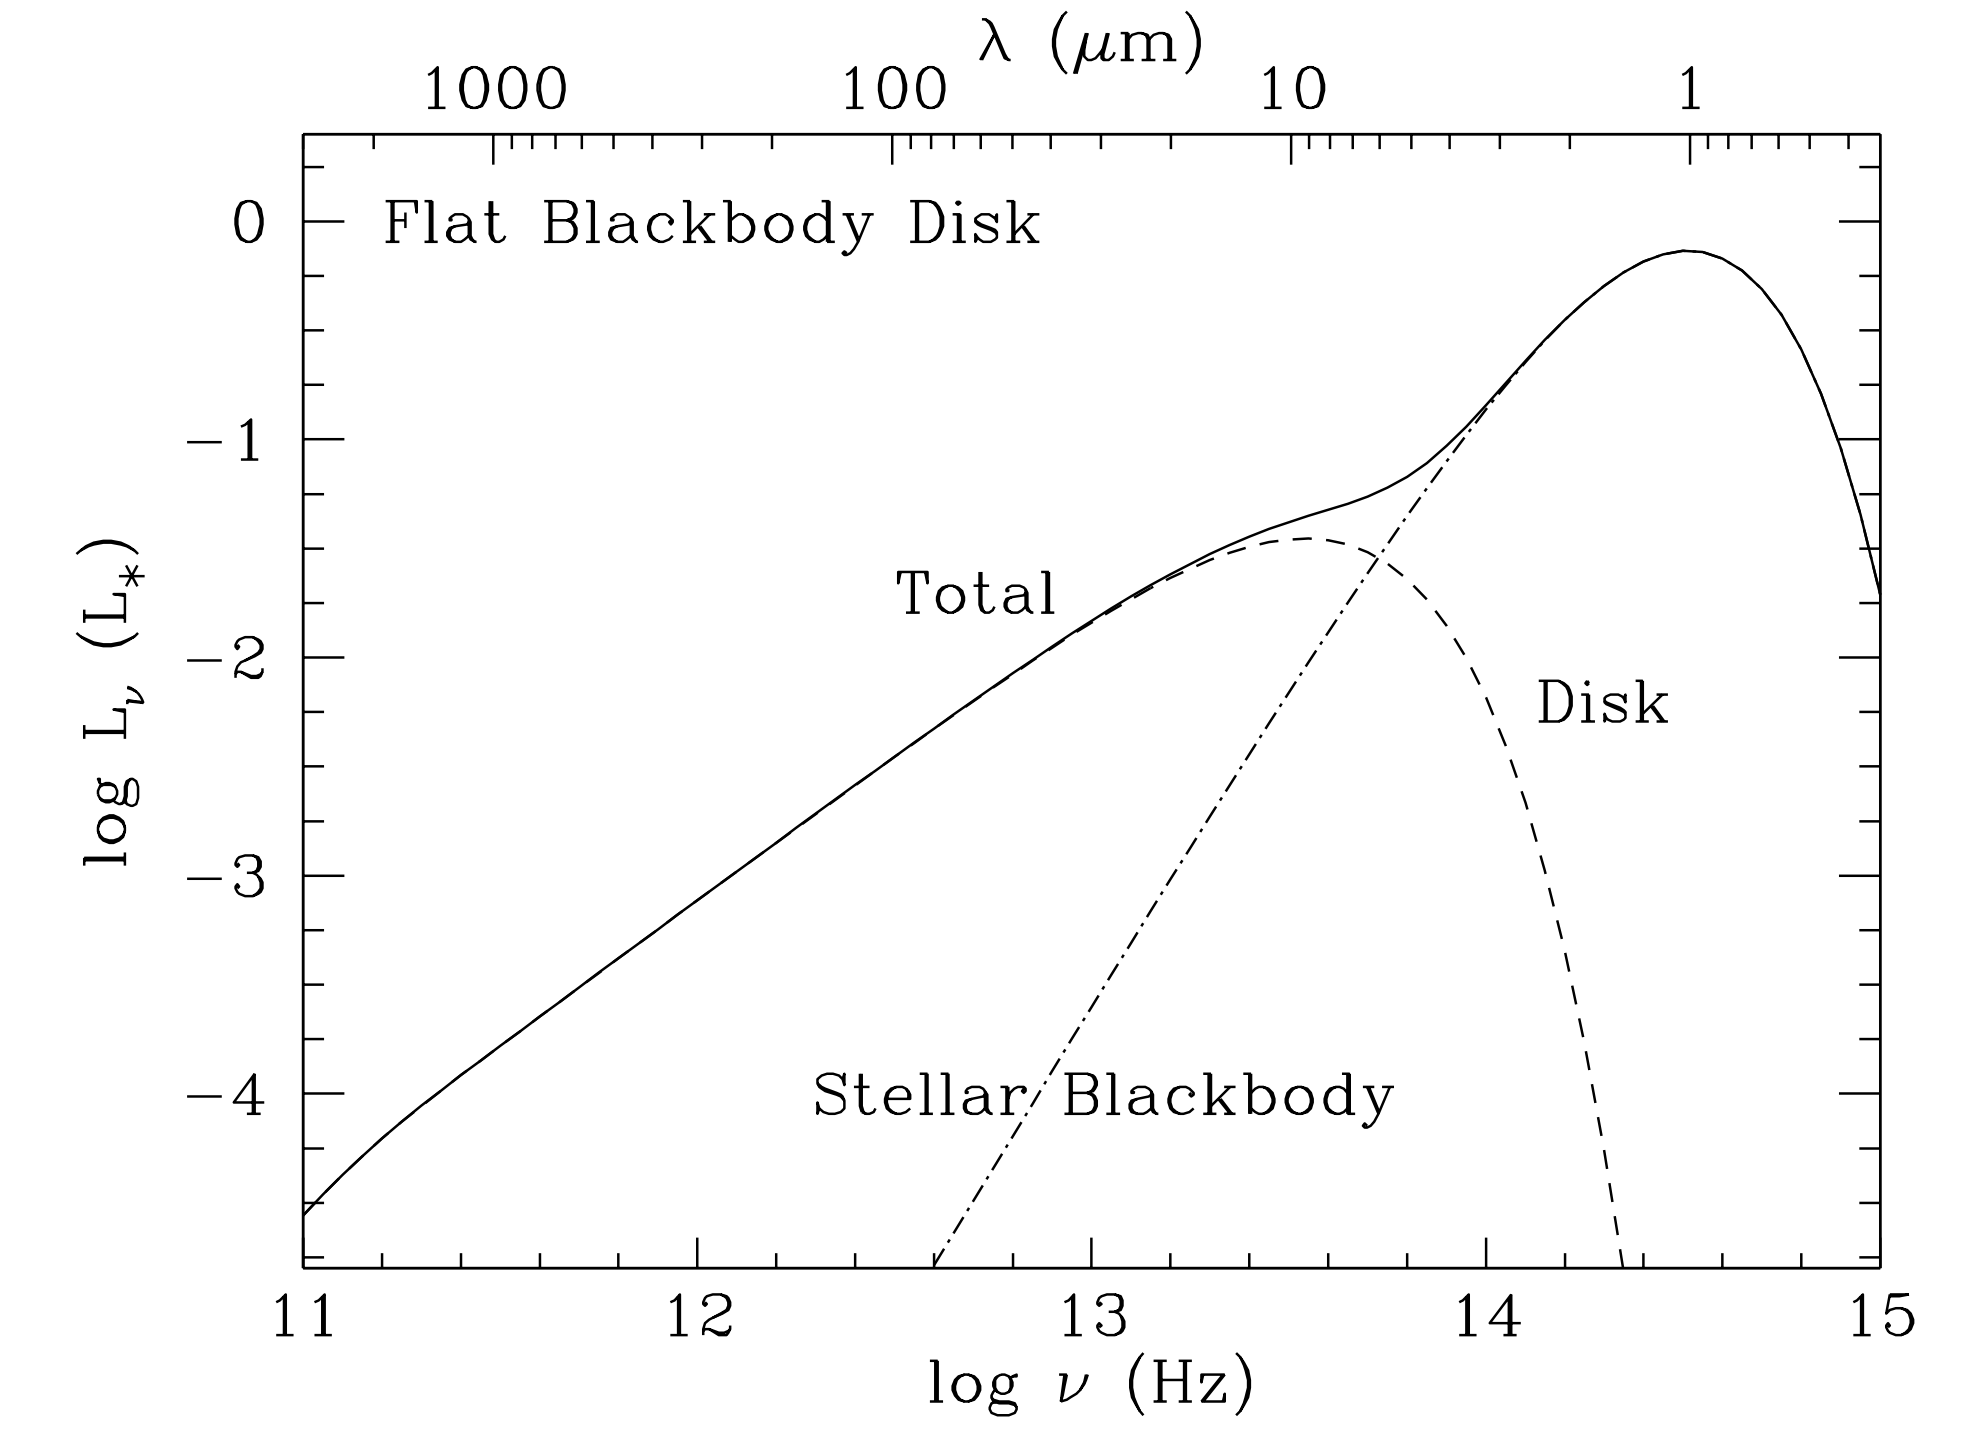
\includegraphics[width=7.5cm]{figures/TT_SED_flat.png}
    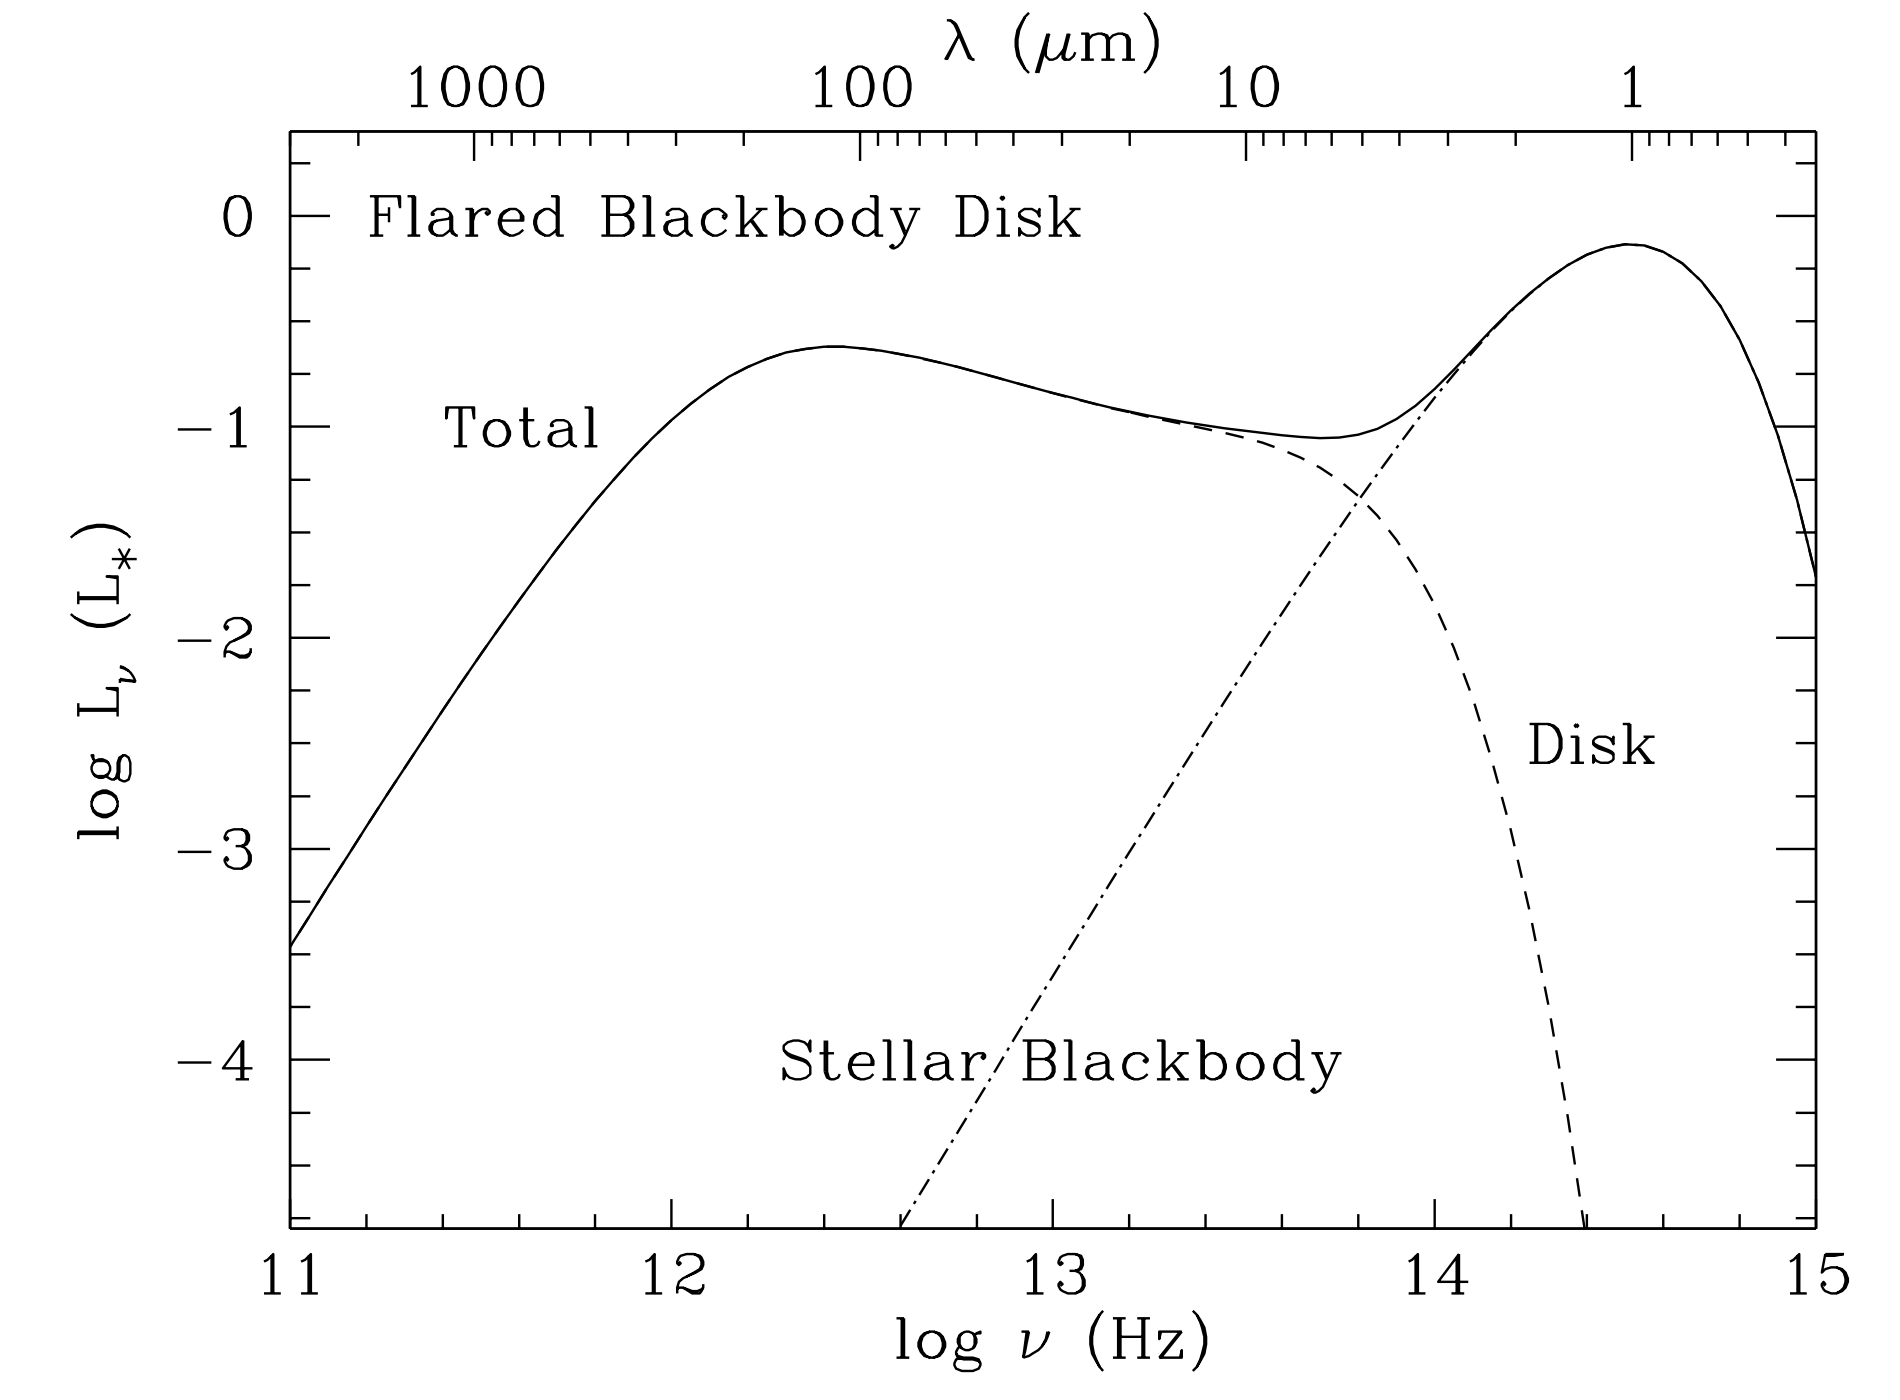
\includegraphics[width=7.5cm]{figures/TT_SED_flared.png}
    \caption{\footnotesize{(\textbf{Left}): SED for the flat blackbody disk, with contributions from star and disk identified. The $n=4/3$ law is evident between $30\,\mu{\rm m}$ and $1\,{\rm mm}$. The turnover near $1\,{\rm mm}$ is due to the truncation of the disk at $a_0=270\,{\rm AU}$. (\textbf{Right}): SED for the flared blackbody disk. At mid-IR wavelengths, $L_\nu\propto\nu^{-2/3}$. At longer wavelengths, $L_\nu\propto\nu^3$. Figure taken from Chiang \& Goldreich (1997).}}
    \label{fig:ttsed}
\end{figure}

{\noindent}\textbf{Flared geometry}: We retain the assumption that the disk radiates as a blackbody and consider the consequences of vertical hydrostatic equilibrium in a gravitational field $g=\Omega^2z$.

{\noindent}The disk temperature $T_e$ is still given by

\begin{align*}
    T_e \sim \left(\frac{\alpha}{2}\right)^{1/4} \left(\frac{R_{\rm TT}}{a}\right)^{1/2} T_{\rm TT} ~ [{\rm K}],
\end{align*}

{\noindent}but now the grazing angle $\alpha$ takes the more general form

\begin{align*}
    \alpha \sim \frac{0.4R_{\rm TT}}{a} + a\frac{{\rm d}}{{\rm d}a} \left(\frac{H}{a}\right) ~ [{\rm deg}],
\end{align*}

{\noindent}where $H$ is the height of the visible photosphere above the disk midplane.

{\noindent}Taking the gas to be isothermal at temperature $T_e$ yields a Gaussian density profile

\begin{align*}
    \frac{n}{n_0} = \exp \left(-\frac{z^2}{2h^2}\right) ~ [{\rm dimensionless}],
\end{align*}

{\noindent}where

\begin{align*}
    \frac{h}{a} = \left(\frac{T_e}{T_c}\right)^{1/2} \left(\frac{a}{R_{\rm TT}}\right)^{1/2} ~ [{\rm dimensionless}].
\end{align*}

{\noindent}The temperature $T_c$ is a measure of the gravitational potential at the surface of the central star;

\begin{align*}
    T_c \equiv \frac{GM_{\rm TT}\mu}{k_BR_{\rm TT}} \sim 8\times10^6 ~ [{\rm K}],
\end{align*}

{\noindent}with $\mu$ being the mean molecular weight of the gas. Under the assumption that the dust-to-gas ratio if uniform throughout the disk, we have

\begin{align*}
    \frac{H}{h} = \left[2\ln\left(\frac{n_0}{n_{\rm ph}}\right)\right]^{1/2} ~ [{\rm dimensionless}],
\end{align*}

{\noindent}where $n_{\rm ph}$ is the number density of the photosphere. In the limit of large radius where $\alpha$ is dominated by the flaring term,

\begin{align*}
    \frac{H}{a} \sim 4\left(\frac{T_{\rm TT}}{T_c}\right)^{4/7} \left(\frac{a}{R_{\rm TT}}\right)^{2/7} \sim 0.18a_{\rm AU}^{2/7} ~ [{\rm dimensionless}].
\end{align*}

{\noindent}It is assumed that $H/h=4$; in reality, this factor declines from about $5$ to $4$ between $a_{\rm AU}=3$ to $a_{\rm AU}=4$.

{\noindent}It follows that $\alpha\sim0.005a_{\rm AU}^{-1}+0.05a_{\rm AU}^{2/7}$. Thus, $\alpha$ is minimal at the transition radius $a_{\rm tr}\sim0.4\,{\rm AU}$ with $\alpha_{\rm min}\sim0.05$. Beyond the transition radius, the disk flares until $H\sim a$ at $a_0\sim270\,{\rm AU}$.

{\noindent}The SED for the flared blackbody disk truncated at $a_0$ is shown in Figure \ref{fig:ttsed} (right). At wavelengths between $10$ and $100\,\mu{\rm m}$, the disk emission follows the scaling relation $L_\nu\propto\alpha L_{\rm TT}\sim0.1(\nu/10^{13}\,{\rm Hz}^{-2/3}L_{\rm TT})$. Longward of $300\,\mu{\rm m}$ in the Rayleigh-Jeans regime, the SED varies as $\nu^3$.

% --------------------------------------------------------------
%               15. 
% --------------------------------------------------------------

\newpage
\subsection{Question 15}

What are the primary origins of the heat lost to space by infrared luminosity of Jupiter, Earth, and Io?\footnote{Answer shamelessly stolen from Miranda.}

\subsubsection{Short answer}

\begin{enumerate}
    \item \textbf{Jupiter}: Found to emit $\sim2.5$ times the energy that it absorbs from the Sun, which suggests that it might still be contracting (consistent with a rate of $0.5\,{\rm mm\,century^{-1}}$) or undergoing differentiation of hydrogen and helium in the atmosphere.
    \item \textbf{Earth}: Main source of IR luminosity is re-radiated Solar flux. The Earth has an albedo of $\sim0.3$, which means it absorbs $\sim70\%$ of the incident Solar radiation.
    \item \textbf{Io}: Tidal heating via internal tidal forces not only supplies the IR luminosity of Io, but maintains its strong volcanic activity.
\end{enumerate}

\subsubsection{Follow-up Questions}

\begin{itemize}
    \item Saturn is a gas giant like Jupiter; is it also believed to be contracting?
    \item What supplies the tidal heating of Io (i.e., what is physically happening)?
\end{itemize}


% --------------------------------------------------------------
%               16. 
% --------------------------------------------------------------

\newpage
\subsection{Question 16}

Explain the observational problem of radius inflation for hot Jupiters and describe two possible solutions.

\subsubsection{Short answer}

Planet structure and evolution models had predicted there should be a clear maximum size for evolved giant planets. In the absence of any additional energy source, even a completely gaseous planet should never be larger than $\sim1.2\,{\rm R_J}$ by the time it is several billion years old. Nonetheless, at short orbital periods there are now dozens of highly inflated hot Jupiters, some with radii that are almost $\sim2\,{\rm R_J}$. Moreover, not all hot Jupiters are inflated to the same degree; instead, we see that even among the highly irradiated gas giants, the most irradiated planets are much more inflated than those that are slightly further out. There are several possible explanations for this observational problem:

\begin{itemize}
    \item invoking an extra heat source for the interior, perhaps caused by orbital tidal heating, ``kinetic heating'' in which wind energy is converted into heat, obliquity tides when in a Cassini state, Ohmic dissipation, or penetration of gravity waves into the planetary interior that then dissipate at depth
    \item enhanced atmospheric opacities which delay the loss of heat and entropy and retain an inflated atmosphere
    \item a magnetohydrodynamic mechanism with Ohmic heating and attendant magnetic braking of the velocity field at sufficient atmospheric ionization fraction
\end{itemize}

\subsubsection{Additional context}

Since the discovery of the first transiting hot Jupiters, models have sought to explain the anomalously large radii of highly irradiated gas giants. We now know that the size of hot Jupiter radius anomalies scales strongly with a planet's level of irradiation and numerous models like tidal heating, ohmic dissipation, and thermal tides have since been developed to help explain these inflated radii. In general, however, these models can be grouped into two broad categories: models that directly inflate planetary radii by depositing a fraction of the incident irradiation into the interior and models that simply slow a planet's radiative cooling, allowing it to retain more heat from formation and thereby delay contraction.

% --------------------------------------------------------------
%               17. 
% --------------------------------------------------------------

\newpage
\subsection{Question 17}

Explain the effects of an atmosphere on a planet's surface temperature and the position of the “habitable zone”. What special considerations must one make for habitability around M-type stars?

\subsubsection{Short answer}

Answer.

\subsubsection{Additional context}

Additional context.

% --------------------------------------------------------------
%               18. 
% --------------------------------------------------------------

\newpage
\subsection{Question 18}

Explain the process of nuclear fusion and give two examples of important fusion processes that affect the lives of stars.

\subsubsection{Short answer}

Most observed stars (including the Sun) live on \textbf{thermonuclear fusion}. In such nuclear reactions, induced by the thermal motion, several lighter nuclei fuse to form a heavier one.

\subsubsection{Additional context}

\textbf{General properties of the nucleus}: The notion that the atom can be viewed as being composed of a nucleus surrounded by a cloud of electrons which are confined to shells led to a very successful theory of atomic spectra. A very similar picture can be postulated for the nucleus itself, namely, that nucleons are arranged in shells within the nucleus and undergo transitions from one excited state (shell) to another subject to the same sort of selection rules that govern atomic transitions. The origin of the shell structure of any nucleus is that nucleons are fermions and therefore must obey the \textbf{Pauli Exclusion Principle}, just as the atomic electrons do. Thus, only two protons or two neutrons may occupy a specific cell in phase space (protons and neutrons have the same spin as electrons, so each species can have two of its kind in a quantum state characterized by the spatial quantum numbers).

{\noindent}However, the nucleons are much more tightly bound in the nucleus than the electrons in the atom. Whereas the typical ionization energy of an atom can be measured in tens to thousands of electron volts, the typical binding energy of a nucleon in the nucleus is several million electron volts. This large binding energy and the Pauli Exclusion Principle can be used to explain the stability of the neutron in nuclei. Although free neutrons beta-decay to protons (and an electron and an electron anti-neutrino) with a half-life of about 10 min, neutrons appear to be stable when they are in nuclei. If neutrons did decay, the resulting proton would have to occupy one of the least tightly bound proton shells, which frequently costs more energy than is liberated by the beta decay of the neutron. Thus, unless the neutron decay can provide sufficient energy for the decay products to be ejected from the nucleus, the neutron must remain in the nucleus as a stable entity.

{\noindent}\textit{For a nucleus to be stable, its mass must be less than the sum of the masses of any possible combination of its constituents}. Thus, $^5$Li is not stable, whereas $^4$He is. However, note that the instability of mass-5 nuclei posed one of the greatest barriers of the century to the understanding of the evolution of stars. The nuclear evolution beyond mass 5 was finally solved by Fred Hoyle, who showed that the triple-$\alpha$ process could actually initiate synthesis of all the nuclei heavier than mass 12.

{\noindent}Most observed stars (including the Sun) live on so-called thermonuclear fusion. In such nuclear reactions, induced by the thermal motion, several lighter nuclei fuse to form a heavier one. Before this process, the involved nuclei $j$ have a total mass ($\sum m_j$) different from that of the product nucleus ($m_y$). This difference is called the \textbf{mass defect}:

\begin{align*}
    \Delta m = \sum m_j - m_y ~ [{\rm kg}].
\end{align*}

{\noindent}This mass defect is converted into energy according to Einstein's formula

\begin{align*}
    E = \Delta m c^2 ~ [{\rm eV}]
\end{align*}

{\noindent}and is available (at least partly) for the star's energy balance. Usually for such a reaction to happen, it must be exothermic. That is, the rest energy of the initial constituents of the reaction must exceed that of the products:

\begin{align*}
    \Delta mc^2>0 ~ [{\rm eV}].
\end{align*}

{\noindent}An example is the series of reactions called \textbf{hydrogen burning}, where four hydrogen nuclei $^1$H with a total mass $4\times1.0079\,{\rm amu}$ (atomic mass units, physical scale) are transformed into one $^4$He nucleus of $4.0026\,{\rm amu}$. Atomic masses are given for the neutral atoms (i.e., for the nucleus plus all electrons). However, since the electron mass is only $1/1823\,{\rm amu}$, we will assume that masses of nuclei are the same as the atomic masses. Obviously $2.9\times10^{-2}\,{\rm amu}$ per produced $^4$He nucleus have ``disappeared'' during the fusion of the four protons, which is roughly $0.7\%$ of the original masses and which corresponds to an energy of about $27.0\,{\rm MeV}$. As usual in nuclear physics, as the unit of energy, we take the electron volt ${\rm eV}$ ($1\,{\rm eV}=1.6018\times10^{-12}\,{\rm erg}$) with the following equivalences:

\begin{align*}
    1\,{\rm keV} \equiv 1.1606\,{\rm K} \\
    931.49\,{\rm MeV} \equiv 1\,{\rm amu}.
\end{align*}

{\noindent}The Sun's luminosity corresponds to a mass loss rate of $L_\odot/c2=4.26\times10^{12}\,{\rm g\,s^{-1}}$, which appears to be a lot, especially if it is read as ``more than four million metric tons per second''. If a total of $1\,{\rm M_\odot}$ of hydrogen were converted into $^4$He, then the disappearing $0.7\%$ of this mass would be $1.4\times10^{31}\,{\rm g}$, which could balance the Sun's present mass loss by radiation for about $3\times10^{18}\,{\rm s}\sim10^{11}\,{\rm yr}$.

{\noindent}The deficiency of mass is just another aspect of the fact that the involved nuclei have different binding energies ($E_B$). This is the energy required to separate the nucleons (protons and neutrons in the nucleus) against their mutual attraction by the strong, but short-range, nuclear forces. Or else, the binding energy is the energy gained if they are brought together from infinity (which starts here at any distance large compared with, say, $10^{-12}\,{\rm cm}$, the scale of a nuclear size).

{\noindent}Consider a nucleus of mass $M_{\rm nuc}$ and atomic mass number $A$ (the integer \textbf{atomic weight}): it may contain $Z$ protons of mass $m_p$ and $(A-Z)$ neutrons of mass $m_n$. Its binding energy is then related to these masses by

\begin{align*}
    E_B &= \Delta mc^2 ~ [{\rm MeV}] \\
    E_B &= [(A-Z)m_n+Zm_p-M_{\rm nuc}]c^2  ~ [{\rm MeV}].
\end{align*}

{\noindent}When comparing different nuclei, it is more instructive to consider the average binding energy per nucleon,

\begin{align*}
    f = \frac{E_B}{A} ~ [{\rm MeV}]
\end{align*}

{\noindent}which is also called the \textbf{binding fraction}. With the exception of hydrogen, typical values are around $8\,{\rm MeV}$, with relatively small differences for nuclei of very different $A$. This shows that the short-range nuclear forces due to a nucleon mainly affect the nucleons in its immediate neighbourhood only, such that with increasing $A$, a saturation occurs rather than an increase of $f$ proportional to $A$. An idealized plot of $f$ against $A$ is shown in Figure \ref{fig:nucleonbindingenergy} (the curve zigzags around this smoothed curve as a consequence of the shell structure of the nucleus and pair effects).

\begin{figure}[t]
    \floatbox[{\capbeside\thisfloatsetup{capbesideposition={right,top},capbesidewidth=4cm}}]{figure}[\FBwidth]
    {\caption{\footnotesize{The average binding energy per nucleon $f$ as a function of atomic mass number $A$. Figure taken from \href{https://physics.stackexchange.com}{https://physics.stackexchange.com}.}}
    \label{fig:nucleonbindingenergy}}
    {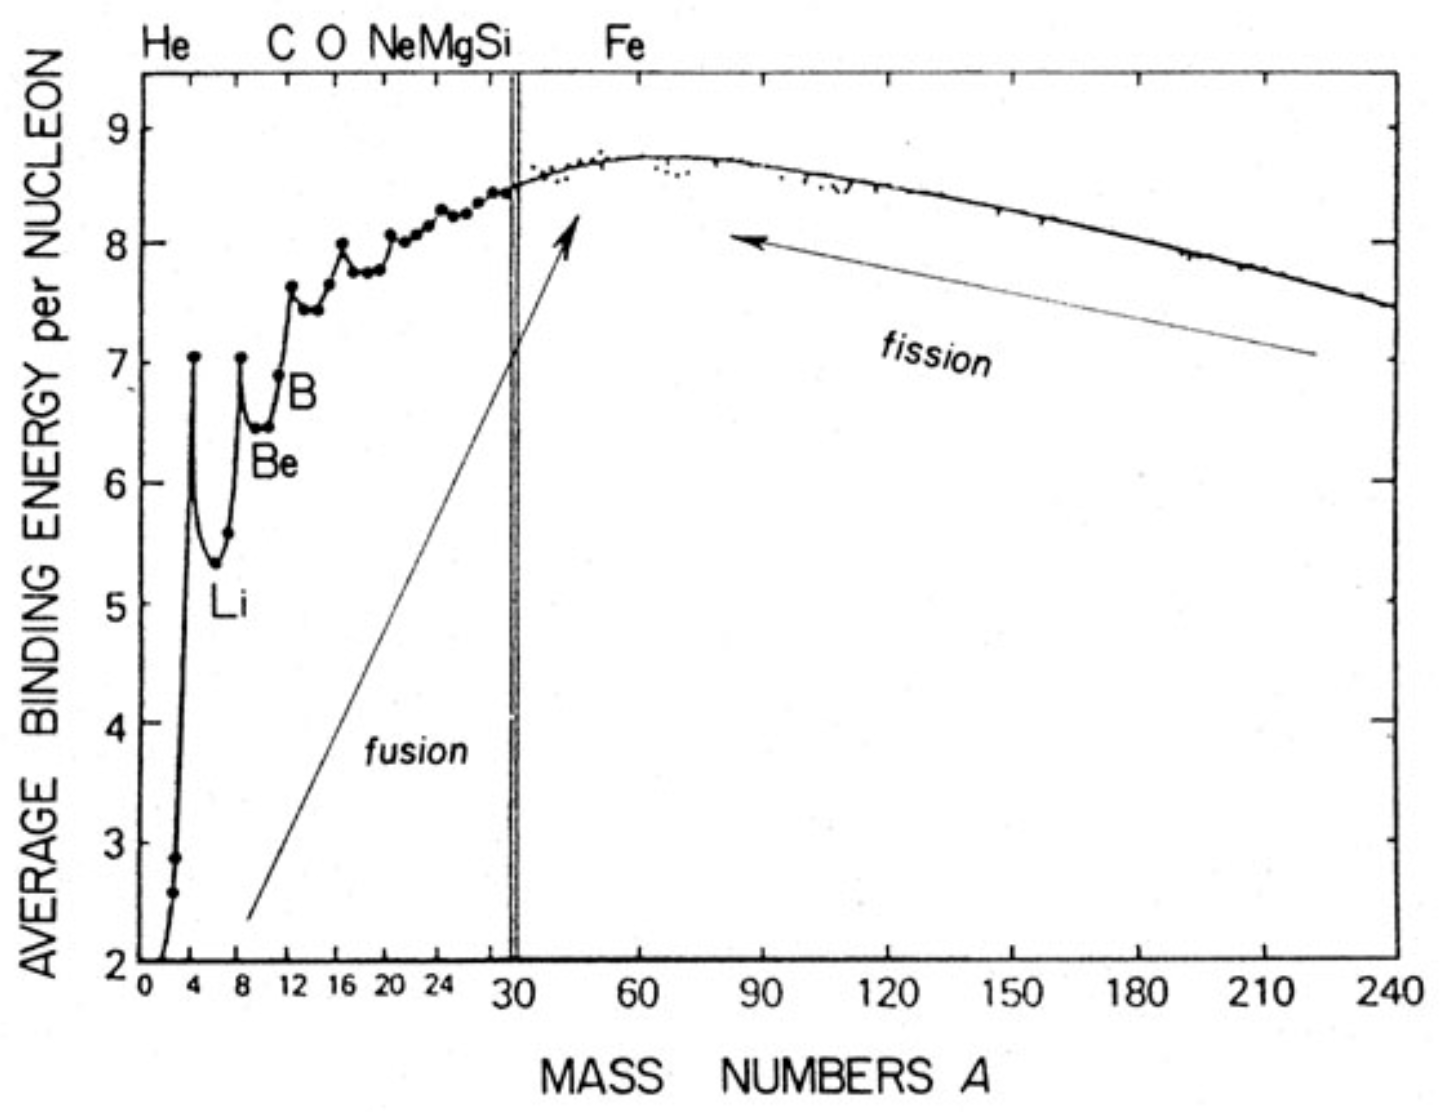
\includegraphics[width=12cm]{figures/NucleonBindingEnergy.png}}
\end{figure}

{\noindent}With increasing $A$, $f(A)$ rises steeply from hydrogen, then flattens out and reaches a maximum of $8.5\,{\rm MeV}$ at $A=56(^{56}{\rm Fe})$, after which it drops slowly with increasing $A$. The increase for $A<56$ is a surface effect: particles at the surface of the nucleus experience less attraction by nuclear forces than those in the interior, which are completely surrounded by other particles. And in a densely packed nucleus, the surface area increases with radius slower than the volume (i.e. the number $A$) such that the fraction of surface particles drops. With increasing $A$, the number $Z$ of protons also increases (the addition of neutrons only would require higher energy states, because the Pauli exclusion principle excludes more than two identical neutrons, and the nuclei would be unstable). The positively charged protons experience a repulsive force which is far-reaching and therefore does not show the saturation of the nuclear forces. This increasing repulsion by the Coulomb forces brings the curve in Figure \ref{fig:nucleonbindingenergy} down again for $A>56$.

{\noindent}Around the maximum, at $^{56}{\rm Fe}$, we have the most tightly bound nuclei. In other words, the nucleus of $^{56}{\rm Fe}$ has the smallest mass per nucleon, so that any nuclear reaction bringing the nucleus closer to this maximum will be exothermic (i.e., it will release energy). There are two ways of doing this:

\begin{enumerate}
    \item By fission of heavy nuclei, which happens, for example, in radioactivity.
    \item By fusion of light nuclei, which is the prime energy source of stars (and possibly ours too in the future).
\end{enumerate}

{\noindent}Clearly, both reach an end when one tries to extend them over the maximum of $f$, which is therefore a natural finishing point for the stellar nuclear engine. So if a star initially consisted of pure hydrogen, it could gain a maximum of about $8.5\,{\rm MeV}$ per nucleon by fusion to $^{56}{\rm Fe}$, but $6.7\,{\rm MeV}$ of these are already used up when $^4$He is built up in the first step.

\begin{figure}[t]
    \centering
    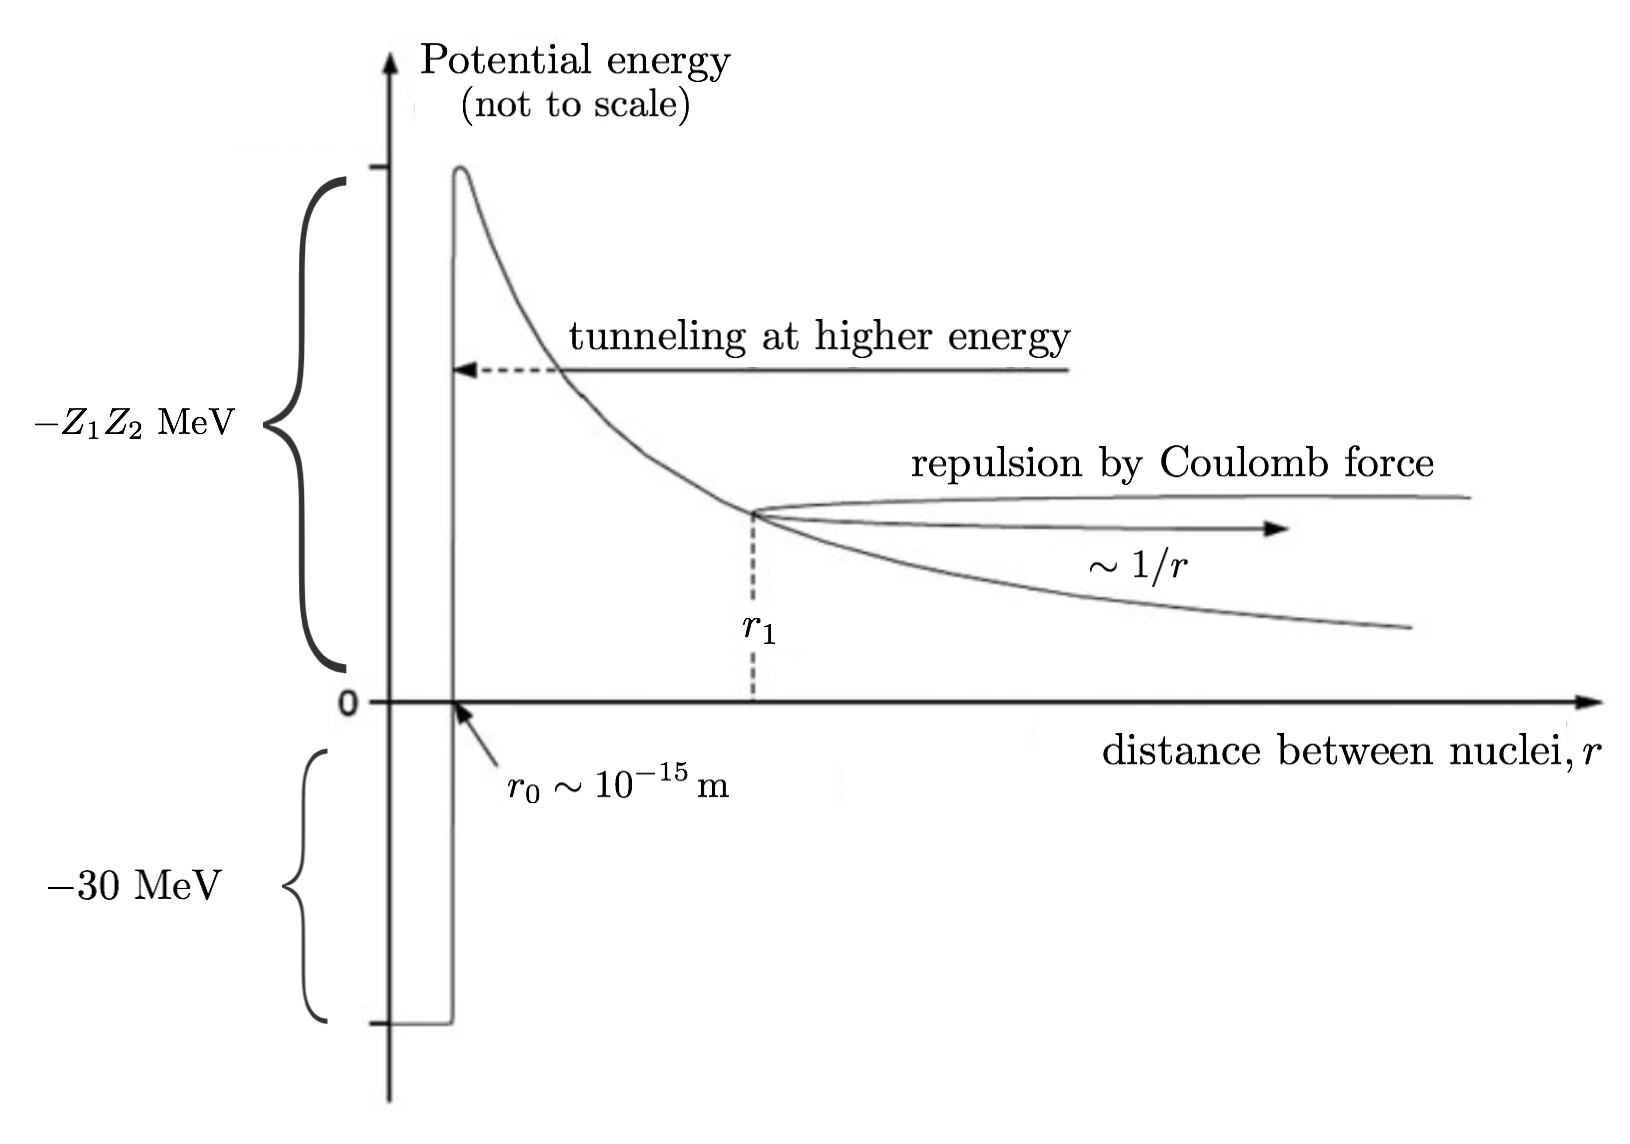
\includegraphics[width=14cm]{figures/CoulombBarrier.png}
    \caption{\footnotesize{Sketch of the potential over the distance $r$ from the nuclear centre. Nuclear attraction dominates for $r<r_0$ and Coulomb repulsion for $r>r_0$. Figure adapted from Collins (2003) and \href{https://physics.stackexchange.com}{https://physics.stackexchange.com}.}}
    \label{fig:coulombbarrier}
\end{figure}

{\noindent}In order to obtain a fusion of charged particles, they have to be brought so close to each other that the strong, but very short-ranged, nuclear forces dominate over the weaker, but far-reaching, Coulomb forces. The counteraction of these two forces leads to a sharp potential jump at the interaction radius (Figure \ref{fig:coulombbarrier}):

\begin{align*}
    r_0 \approx A^{1/3}1.44\times10^{-13} ~ [{\rm fm}]
\end{align*}

{\noindent}(the \textbf{nuclear radius} of the order of \textbf{femtometer}, $1\,{\rm fm}=10^{-13}\,{\rm cm}$). For distances less than $r_0$, the nuclear attraction dominates and provides a potential drop of roughly $30\,{\rm MeV}$, while beyond $r_0$, the repulsive Coulomb forces for particles with charges $Z_1$ and $Z_2$ yield

\begin{align*}
    E_{\rm Coul} = \frac{Z_1Z_2e^2}{r} ~ [{\rm MeV}].
\end{align*}

{\noindent}The height of the Coulomb barrier $E_{\rm Coul}(r_0)$ is typically of the order

\begin{align*}
    E_{\rm Coul}(r_0) \approx Z_1Z_2 ~ [{\rm MeV}].
\end{align*}

{\noindent}If, in the stationary reference frame of the nucleus, a particle at infinity has kinetic energy $E_1$, it can come classically only to a distance $r_1$ given by $E_1=E_{\rm Coul}(r_1)$, as indicated in Figure \ref{fig:coulombbarrier}. Now, the kinetic energy available to particles in stellar interiors is that of their thermal motion, and hence the reactions triggered by this motion are called thermonuclear. Since in normal stars we observe a slow energy release rather than a nuclear explosion, we must certainly expect the average kinetic energy of the thermal motion, $E_{\rm th}$, to be considerably smaller than $E_{\rm Coul}(r_0)$. For $T\sim10^7\,{\rm K}$ estimated for the solar centre, $k_BT$ is only $10^3\,{\rm eV}$ (i.e., $E_{\rm th}$ is smaller than the Coulomb barrier by a factor of roughly $10^3$. This is in fact so low that, with classical effects only, we can scarcely expect any reaction at all. In the high-energy tail of the Maxwell-Boltzmann distribution, the exponential factor drops here to $\exp(-1000)\approx10^{-434}$, which leaves no chance for the ``mere'' $10^{57}$ nucleons in the whole Sun (and even for the $\sim10^{80}$ nucleons in the whole visible Universe)!

{\noindent}The only possibility for thermonuclear reactions in stars comes from a quantum-mechanical effect found by G. Gamow: there is a small but finite probability of penetrating (\textbf{quantum tunnelling}) through the Coulomb barrier, even for particles with $E<E_{\rm Coul}(r_0)$. This tunnelling probability varies as 

\begin{align*}
    P = CE^{-1/2}\exp^{-2\pi\eta}, ~~~ \eta=\sqrt{\frac{m}{2}}\frac{Z_1Z_2e^2}{\hbar\sqrt{E}}.
\end{align*}

{\noindent}Here $\hbar$ is the \textbf{reduced Planck constant} $h/2\pi$ and $m$ the \textbf{reduced mass}. The factor $C$ is a constant that depends only on the properties of the two colliding nuclei. The exponent $2\pi\eta$ is obtained as the only $E$-dependent term in an approximate evaluation of the integral over $\hbar^{-1}\sqrt{2m(E_{\rm Coul}-E)}$, which is extended from $r_0$ to the distance of closest approach (i.e., where $E=E_{\rm Coul}$). For $Z_1Z_2=1$ and $T=10^7\,{\rm K}$, $P$ is of the order of $10^{-20}$ for particles with average kinetic energy $E$ and steeply increases with $E$ and decreases with $Z_1Z_2$. Therefore, for temperatures as ``low'' as $10^7\,{\rm K}$, only the lightest nuclei (with smallest $Z_1Z_2$) have a chance to react. For reactions of heavier particles, with larger $Z_1Z_2$, the energy (i.e., the temperature) has to be correspondingly larger to provide a comparable quantum tunneling probability. This will result in well-separated phases of different nuclear burning during the star's evolution.

{\noindent}\textbf{Nuclear reaction rates}: Consider collisions between two different kinds of particles with a number density in phase space of ${\rm d}N_1$ and ${\rm d}N_2$. To obtain the number of collisions per second per unit volume, we must integrate over all available velocity space. That is, we must sum over the collisions between particles so that the collision rate $r$ is

\begin{align*}
    r = \int\int v\sigma(v){\rm d}N_1(\vec{v}_1){\rm d}N_2(\vec{v}_2) ~ [{\rm s^{-1}\,m^{-3}}].
\end{align*}

{\noindent}Let us assume that the velocity distributions of both kinds of particles are given by Maxwellian velocity distributions

\begin{align*}
    {\rm d}N = N \left(\frac{m}{2\pi k_BT}\right)^{3/2} e^{-mv^2/(2k_BT)}{\rm d}v,
\end{align*}

{\noindent}so that the collision rate equation becomes

\begin{align*}
    r = N_1N_2 \left(\frac{m_1}{2\pi k_BT}\right)^{3/2} \left(\frac{m_2}{2\pi k_BT}\right)^{3/2} \int\limits_{-\infty}^\infty \int\limits_{-\infty}^\infty \left(\frac{-m_1v_1^2}{2k_BT}+\frac{-m_2v_2^2}{2k_BT}\right) v\sigma(v){\rm d}\vec{v}_1{\rm d}\vec{v}_2 ~ [{\rm s^{-1}\,m^{-3}}].
\end{align*}

{\noindent}If we transform to the center-of-mass coordinate system, assuming the velocity field is isotropic, so that the triple integrals can be written as spherical ``velocity volumes'', then we can rewrite this in terms of the center of
mass velocity $v_0$ and the relative velocity $v$ as

\begin{align*}
    r = N_1N_2 \left(\frac{m_1}{2\pi k_BT}\right)^{3/2} \left(\frac{m_2}{2\pi k_BT}\right)^{3/2} \int\limits_0^\infty \int\limits_0^\infty \exp\left[- \frac{(m_1+m_2)v_0^2+\tilde{m}v^2}{2k_BT} \right] v\sigma(v)4\pi v_0^2(4\pi v^2){\rm d}v_0{\rm d}v ~ [{\rm s^{-1}\,m^{-3}}],
\end{align*}

{\noindent}where

\begin{align*}
    \tilde{m} &= \frac{m_1m_2}{m_1+m_2} ~ [{\rm kg}] \\
    \vec{v}   &= \vec{v}_1-\vec{v}_2 ~ [{\rm m\,s^{-1}}] \\
    \vec{v}_0 &= \frac{m_1\vec{v}_1+m_2\vec{v}_2}{m_1+m_2} ~ [{\rm m\,s^{-1}}].
\end{align*}

{\noindent}The integral over $_0v$ is analytic and is

\begin{align*}
    \int\limits_0^\infty \exp\left[-\frac{(m_1+m_2)v_0^2}{2k_BT}\right] 4\pi v_0^2{\rm d}v_0 = \left(\frac{2\pi k_BT}{m_1+m_2}\right)^{3/2}
\end{align*}

{\noindent}which reduces $r$ to 

\begin{align*}
    r = N_1N_2 \left(\frac{\tilde{m}}{2\pi k_BT}\right)^{3/2} \int\limits_0^\infty \exp\left[-\frac{\tilde{m}v^2}{2k_BT}\right] v\sigma(v) (4\pi v^2) {\rm d}v ~ [{\rm s^{-1}\,m^{-3}}].
\end{align*}

{\noindent}Since the \textit{relative} kinetic energy in the center of mass system is $E=mv^2/2$, we can rewrite this in terms of an average reaction cross section $\langle\sigma(v)v\rangle$, so that

\begin{align*}
    r = N_1N_2\langle\sigma(v)v\rangle
\end{align*}

{\noindent}where

\begin{align*}
    \langle\sigma(v)v\rangle = \frac{2}{\sqrt{\pi}} \left(\frac{1}{k_BT}\right)^{3/2} \int\limits_0^\infty \exp\left(\frac{-E}{k_BT}\right)\sigma(v)v\sqrt{E}{\rm d}E = \int\limits_0^\infty n(E)v\sigma(v){\rm d}E.
\end{align*}

{\noindent}Thus $\langle\sigma(v)v\rangle$ is the ``relative energy'' weighted average of the collision probability of particle $1$ with particle $2$. When this average cross section is written, the explicit dependence on velocity is usually omitted, so that

\begin{align*}
    \langle\sigma v\rangle \equiv \langle\sigma(v)v\rangle.
\end{align*}

{\noindent}If the collisions involve identical particles, then the number of distinct pairs of particles is $N(N-1)/2$ so the factor of $N_1N_2$ is replaced by $N^2/2$.

{\noindent}If we call the \textbf{energy produced per reaction} $Q$, we can write the energy produced per gram of stellar material as

\begin{align*}
    \epsilon = \frac{r_{1,2}Q}{\rho} = \frac{N_1N_2\langle\sigma v\rangle}{\rho} ~ [{\rm eV\,g^{-1}}].
\end{align*}

{\noindent}The number densities can be replaced with the more common fractional abundances by mass to get

\begin{align*}
    \epsilon = \left[ N_A^2Q \langle\sigma v\rangle \left(\frac{X_1}{m_1}\right) \left(\frac{X_2}{m_2}\right) \right] \rho ~ [{\rm eV\,g^{-1}}]
\end{align*}

{\noindent}where $N_A$ is \textbf{Avogadro's number}. Since $\langle\sigma v\rangle$ is a complicated function of temperature and must be obtained numerically, this is usually approximated numerically as

\begin{align*}
    \epsilon \approx \epsilon_0\rho T^\nu ~ [{\rm eV\,g^{-1}}]
\end{align*}

{\noindent}where

\begin{align*}
    \epsilon_0 = N_A^2Q \langle\sigma v\rangle \left(\frac{X_1}{m_1}\right) \left(\frac{X_2}{m_2}\right) \frac{1}{T_0^\nu} ~ [{\rm eV\,g^{-2}\,cm^3\,K^{-1}}].
\end{align*}

{\noindent}Here $\nu$ itself is very weakly dependent on the temperature. Most of the important energy production mechanisms have this form. The approximation $\epsilon\approx\epsilon_0\rho T^\nu$ expresses the energy generated for a specific energy generation mechanism in terms of the state variables $T$ and $\rho$. This is what we were after. Formulas such as these, where $\epsilon_0$ has been determined, will enable us to determine the energy produced throughout the star in terms of the state variables. Let us now consider a few of the specific nuclear reactions for which we have expressions of the type given by this equation of $\epsilon_0$.

{\noindent}\textbf{Specific nuclear reactions}: The nuclear reactions that provide the energy for MS stars all revolve on the conversion of hydrogen to helium. However, this is accomplished by a variety of ways. We may divide these ways into two groups. The first is known as the \textbf{proton-proton cycle} (p-p cycle) and it begins with the conversion of two hydrogen atoms to deuterium. Several possibilities occur on the way to the production of $^4$He. These alternate options are known as \textbf{P2-P6 cycles}. In addition to the proton-proton cycle, a series of nuclear reactions involving carbon, nitrogen, and oxygen also can lead to the conversion of hydrogen to helium with no net change in the abundance of C, N, and O. For this reason, it is known as the \textbf{CNO cycle}. These reactions and their side chains are given below in Table \ref{table:nuclearreactions}:

\begin{table}[t]
\begin{tabular}{lll|lll}
\hline
Step & $Q$ [MeV] & Proton Cycles & Step & $Q$ [MeV] & CNO Cycles \\
\hline
 1     & 1.18  & $^1{\rm H}(p,\beta,\nu)^2{\rm H}$     & 1       & 1.94  & $^{12}C(p,\gamma)^{13}{\rm N}$ \\
 2     & 5.49  & $^2{\rm H}(p,\gamma)^3{\rm He}$       & 2$^*$   & 1.51  & $^{13}{\rm N}\rightarrow^{13}{\rm C}+\beta^++\nu$ \\
 3     & 12.86 & $^3{\rm He}(^3{\rm He},2p)^4{\rm He}$ & 3       & 7.54  & $^{13}{\rm C}(p,\gamma)^{14}{\rm N}$ \\
 or    &       &                                       & 4       & 7.29  & $^{14}{\rm N}(p,\gamma)^{15}{\rm O}$ \\
 3     & 1.59  & $^3{\rm He}(\alpha,\gamma)^7{\rm Be}$ & 5$^*$   & 1.76  & $^{15}{\rm O}\rightarrow^{15}{\rm N}+\beta^++\nu$ \\
 4     & 0.06  & $^7{\rm Be}(\beta^-,\bar{\nu})^7{\rm Li}\rightarrow^7{\rm Li}(p,\alpha)^4{\rm He}$ & 6     & 4.96 & $^{15}{\rm N}(p,\alpha)^{12}{\rm C}$ \\
 or    &       &         ~~~~~~~~~~~~~~~~~~~~$Q=17.35$ &         &       & $^{15}{\rm N}(p,\gamma)^{16}{\rm O}$ \\
 4     & 0.13  & $^7{\rm Be}(p,\gamma)^8{\rm B}$       & 7       &       & $^{16}{\rm O}(p,\gamma)^{17}{\rm F}$ \\
 5$^*$ & 10.78 & $^8{\rm B}\rightarrow^8{\rm Be}+\beta^++\nu $    & 8$^*$ &  & $^{17}{\rm F}\rightarrow^{17}{\rm O}+\beta^++\nu$ \\
 6$^*$ & 0.09  & $^8{\rm Be}\rightarrow2^4{\rm He}$    & 9       &       & $^{17}{\rm O}(p,\alpha)^{14}{\rm N}$ \\
 or    &       &                                       &         &       & $^{17}{\rm O}(p,\gamma)^{18}{\rm F}$ \\
 3     &       & $^3{\rm He}(\beta^-,\nu^3{\rm H})$    & 10$^*$  &       & $^{18}{\rm F}\rightarrow^{18}{\rm O}+\beta^++\nu$ \\
       &       & $^3{\rm H}(p,\gamma)^4{\rm He}$       & 11      &       & $^{18}{\rm O}(p,\alpha)^{15}{\rm N}$ \\
 4     &       & $^3{\rm H}(^3{\rm He},np)^4{\rm He}$  &         &       & $^{18}{\rm O}(p,\gamma)^{19}{\rm F}$ \\
       &       & $^3{\rm H}(^3{\rm H},2n)^4{\rm He}$   & 12      &       & $^{19}{\rm F}(p,\alpha)^{16}{\rm O}$ \\
\cline{1-3}
\multicolumn{3}{c|}{Triple-$\alpha$ process} \\
\cline{1-3}
 1     & \multicolumn{2}{c|}{$2(^4{\rm He})+(\sim100\,{\rm KeV})\rightarrow^8{\rm Be}^*$} \\
 2     & \multicolumn{2}{c|}{$^8{\rm Be}^*(\alpha,^{12}{\rm C}^*)$} \\
 3     & \multicolumn{2}{c|}{$^{12}{\rm C}^*\rightarrow^{12}{\rm C}+2\gamma+7.656\,{\rm MeV}$} \\
 \hline
\end{tabular}
\caption{Nuclear reactions of the p-p chain and CNO cycle. Asterisk (*) denotes reactions that occur by spontaneous decay and do not depend on the local values of the state variables. Table taken from Collins (2003).}
\label{table:nuclearreactions}
\end{table}

{\noindent}Besides the steps marked with asterisks which denote reactions that occur by spontaneous decay and do not depend on local values of the state variables, the steps that are the important contributors to the energy supply have their contribution (their $Q$ value) indicated. The energy of the neutrinos has not been included since they play no role in determining the structure of normal stars. When the p-p cycle dominates on the lower MS, most of the energy is produced by means of the \textbf{P1 cycle}. \textit{The neutrino produced in the fifth step of the P2 cycle is the high energy neutrino which has been detected, but in unexpectedly low numbers, by the neutrino detection experiments}. In general, the relative importance of the P1 cycle relative to P2 and P3 is determined by the helium abundance, since this governs the branching ratio at step $3$ in the p-p cycle. If $^4$He is absent, it will not be possible to make $^7$Be by capture on $^3$He.

{\noindent}Virtually all the energy of the CNO cycle is produced by step 6 as the production of $^{12}$C from $^{15}$N is strongly favored. However, all the higher chains close with only the net production of $^4$He. The first stage of the P4 cycle is endothermic by $18\,{\rm keV}$ so unless the density is high enough to produce a Fermi energy of $18\,{\rm keV}$, the reaction does not take place. This requires a density of $\rho>2\times10^4\,{\rm g\,cm^{-3}}$ and so will not be important in MS stars. Once $^3$H is produced it can be converted to $^4$He by a variety of processes given in step 4. The last two are sometimes denoted \textbf{P5} and \textbf{P6}, respectively, and are rare.

{\noindent}While the so-called \textbf{triple-$\mathbf{\alpha}$ process} is not operative in MS stars, it does provide a major source of energy during the red-giant phase of stellar evolution. The extreme temperature dependence of the triple-$\alpha$ process plays a crucial role in the formation of low-mass red giants. The $^8$Be$^*$ is unstable and decays in an extremely short time. However, if during its existence it collides with another $^4$He nucleus, $^{12}$C can form, which is stable. The very short lifetime for $^8$Be$^*$ basically accounts for the large temperature dependence since a very high collision frequency is required to make the process productive.

{\noindent}The exponent of the temperature dependence given in $\epsilon\approx\epsilon_0\rho T^\nu$ and the constant $\epsilon_0$ both vary slowly with temperature. This dependence is shown in Table \ref{table:tempdepen}.

\begin{table}[]
\begin{tabular}{llllllll}
\hline
\multicolumn{3}{c}{Proton-Proton} & \multicolumn{2}{c}{CNO Cycle} & \multicolumn{3}{c}{Triple-$\alpha$ Process} \\
\cmidrule(l){1-3} \cmidrule(l){4-5} \cmidrule(l){6-8}
$T_6$ & $\epsilon_0$ & $\nu$ & $\epsilon_0$ & $\nu$ & $T_8$ & $\epsilon_0$ & $\nu$ \\
\hline
$10$  & $7\times10^{-2}$ & $4.60$ & $3\times10^{-4}$ & $22.9$ & $0.8$ & $2\times10^{-12}$ & $49$ \\
$20$  & $1$              & $3.54$ & $4.5\times10^2$  & $18.0$ & $1.0$ & $4\times10^{-8}$ & $41$ \\
$40$  & $9$              & $2.72$ & $3\times10^7$    & $14.1$ & $2.0$ & $15.0$ & $19$ \\
$80$  & $43$             & $2.08$ & $2\times10^{11}$ & $11.1$ & $3.0$ & $6\times10^3$ & $12$ \\
$100$ & --               & --     & $2\times10^{12}$ & $10.2$ & $4.0$ & $10^5$ & $7.9$ \\
\hline
\end{tabular}
\caption{Temperature dependence of $\nu$ and $\epsilon_0$.}
\label{table:tempdepen}
\end{table}

{\noindent}The temperature $T_6$ in Table \ref{table:tempdepen} is given in units of $10^6$. Thus $T_6=1$ is $10^6\,{\rm K}$. It is a general property of these types of reaction rates that the temperature dependence $T^\nu$ ``weakens'' as the temperature increases, while the efficiency $\epsilon_0$ increases. In general, the efficiency of the nuclear cycles rate is governed by the slowest process taking place. In the case of p-p cycles, this is always the production of deuterium given in step 1. For the CNO cycle, the limiting reaction rate depends on the temperature. At moderate temperatures, the production of $^{15}$O (step 4) limits the rate at which the cycle can proceed. However, as the temperature increases, the reaction rates of all the capture processes increase, but the steps involving inverse $\beta$ decay (particularly step 5), which do not depend on the state variables, do not and therefore limit the reaction rate. So there is an upper limit to the rate at which the CNO cycle can produce energy independent of the conditions which prevail in the star. However, at temperatures approaching a billion degrees, other reaction processes not indicated above will begin to dominate the energy generation and will circumvent even the beta-decay limitation.

% --------------------------------------------------------------
%               19. 
% --------------------------------------------------------------

\newpage
\subsection{Question 19}

What is Fermi's Paradox? Explain its logic and assess the current state of the Paradox in light of modern knowledge.

\subsubsection{Short answer}

The Fermi paradox, or Fermi's paradox, named after physicist Enrico Fermi, is the apparent contradiction between the lack of evidence and high probability estimates for the existence of extraterrestrial civilizations. The basic points of the argument, made by physicists Enrico Fermi (1901–1954) and Michael H. Hart (born 1932), are:

\begin{enumerate}
    \item There are billions of stars in the galaxy that are similar to the Sun, and many of these stars are billions of years older than the Solar system.
    \item With high probability, some of these stars have Earth-like planets, and if the Earth is typical, some may have developed intelligent life.
    \item Some of these civilizations may have developed interstellar travel, a step the Earth is investigating now.
    \item Even at the slow pace of currently envisioned interstellar travel, the MW galaxy could be completely traversed in a few million years.
\end{enumerate}

{\noindent}According to this line of reasoning, the Earth should have already been visited by extraterrestrial aliens. In an informal conversation, Fermi noted no convincing evidence of this, leading him to ask, ``Where is everybody?'' There have been many attempts to explain the Fermi paradox, primarily either suggesting that intelligent extraterrestrial life is extremely rare or proposing reasons that such civilizations have not contacted or visited Earth.

\subsubsection{Additional context}

Fermi's paradox presents arguably the greatest challenge for any practical SETI acitivity, as well as one of the least understood of all ``grand questions'' posed in the history of science. As is well known, the key argument follows a lunchtime remark of the great physicist, Enrico Fermi: ``Where is everybody?'' First discussed in print by the Russian space-science pioneer Konstantin Eduardovich Tsiolkovsky, and in recent decades elaborated upon in detail by Viewing, Hart, Tipler and others, the argument presents a formidable challenge for any theoretical framework assuming a naturalistic origin of life and intelligence. As such, this should worry not only a small group of SETI enthusiasts, but challenges some of the deepest philosophical and cultural foundations of modern civilization. It is hard to conceive a scientific problem more pregnant in meaning or richer in connections with the other big questions of science throughout the ages.

{\noindent}Tsiolkovsky, Fermi, Viewing, Hart, and their followers argue on the basis of two premises:

\begin{enumerate}
    \item the absence of extraterrestrials in the Solar System; and
    \item the fact that they have had more than enough time in the history of Galaxy to visit, either in person or through their conventional or self-replicating probes.
\end{enumerate}

{\noindent}Characteristic time for colonization of the Galaxy, according to these investigators, is what we shall call the \textbf{Fermi-Hart timescale}:

\begin{align*}
    t_{\rm FH} = 10^6 - 10^8 ~ [{\rm yr}],
\end{align*}

{\noindent}making the fact that the Solar System is (obviously) not colonized hard to explain, if not for the total absence of extraterrestrial cultures. It is enough for our purposes to contend that this timescale is well-defined, albeit not precisely known due to our ignorance regarding the possibilities and modes of interstellar travel. For comparison, the accepted age of the Earth as an object of roughly present-day mass is

\begin{align*}
    t_\oplus = (4.46\pm0.02)\times10^9 ~ [{\rm yr}].
\end{align*}

{\noindent}The drastic difference between these timescales is one of the ways of formulating Fermi's paradox.

{\noindent}Even more generally, we need not consider the direct physical contact between an extraterrestrial civilization and Earth or the Solar System (insofar as we do not perceive evidence of extraterrestrial visits in the Solar System; however, this is still an act of faith, considering the volume of space comprising our planetary system). It is sufficient to consider a weaker requirement: namely, that no extraterrestrial civilizations are detectable by any means from Earth at present. This includes the detectability of astroengineering or macroengineering projects over interstellar distances. In the words of the great writer and philosopher Stanislaw Lem, who authored some of the deepest thoughts on this topic, Fermi's paradox is equivalent to the ``absence of cosmic miracles'' or the \textit{Silentium Universi} (”cosmic silence”). Following the classic review by Brin (1983), we may introduce \textbf{contact cross-section} as a measure of the probability of contact (by analogy with introduction of cross-sections in atomic and particle physics) and reformulate Fermi's paradox as the question why this cross-section in the MW at present is so small in comparison to what could be naively expected.

{\noindent}Schematically, Fermi's paradox can be represented as

\begin{align*}
    {\rm spatiotemporal\,scales\,of\,the\,Galaxy\,+\,the\,absence\,of\,detected\,extraterrestrial\,civilizations}\\ {\rm (+\,additional\,assumptions)\,\rightarrow\,paradoxical\,conclusion.}
\end{align*}

{\noindent}Here, under spatiotemporal scales we include our understanding of the age of the Galaxy, the Solar System and the ages (incompletely known) of other planetary systems in the MW. The additional assumptions can be further explicated as

\begin{align*}
    {\rm additional\,assumptions\,=\,``naive realism''\,+\,naturalism\,+\,Copernicanism\,+\,gradualism\,+}\\ 
    {\rm non-exclusivity.}
\end{align*}

{\noindent}These assumptions are quite heterogeneous. By ``naive realism'' we denote the working philosophy of most of science (as well as everyday life), implying that there is a material world out there, composed of objects that occupy space and have properties such as size, mass, shape, texture, smell, taste and colour. These properties are usually perceived correctly and obey the laws of physics. In the specific case of Fermi's paradox, the basic premise following from naive realism is that there are, indeed, no traces of extraterrestrial intelligent presence detected either directly or indirectly. We shall discuss below some of the hypotheses for resolving Fermi's paradox which directly violate this realist view; an extreme and ludicrous example (but powerfully present in pop-culture) of such naively anti-realist standpoint is a view that, contrary to scientific consensus, some humans are in contact with extraterrestrial visitors and are conspiring with them. Naive realism and naturalism are methodological assumptions typically in play in any scientific research. Copernicanism and gradualism are somewhat more specific tenets, stemming more from our experiences in the history of physical science than from the general epistemology. \textbf{Copernicanism} (often called the \textbf{Principle of Mediocrity}) in a narrow sense tells us that there is nothing special about the Earth or the Solar System or our Galaxy within large sets of similar objects throughout the Universe. In a somewhat broader sense, it indicates that there is nothing particularly special about us as observers: our temporal or spatial location, or our location in other abstract spaces of physical, chemical, biological, etc., parameters are typical or close to typical. \textbf{Gradualism}, on the other hand, is often expressed as the motto that ``the present is key to the past'' (with corollary that ``the past is key to the future''). This paradigm, emerging from geological science in the 19th century with the work of Charles Lyell (and expanding, through Lyell's most famous pupil, Darwin, into life sciences) has been subject of the fierce criticism in the last quarter of a century or so.

{\noindent}Finally, the role of the non-exclusivity (or ``hardness'' in some of the literature) assumption needs to be elucidated. Non-exclusivity is simply a principle of causal parsimony applied to the set of hypotheses for resolving Fermi's paradox: we should prefer those hypotheses which involve a smaller number of local causes. Fermi's paradox is eminently not resolved by postulating that a single old civilization self-destructs in a nuclear holocaust. Fermi's paradox is resolved by hypothesizing that all civilizations self-destruct soon after developing nuclear weapons, but the major weakness of such a solution is obvious: it requires many local causes acting independently in uniform to achieve the desired explanatory end. In other words, such a solution is exclusive (or ``soft''). As long as we have any choice, we should prefer non-exclusive (or ``hard'') solutions (i.e., those which rely on a small number of independent causes). For instance, the hypothesis that a $\gamma$-ray burst can cause mass extinction over a large portion of the Galaxy and thus arrest evolution toward advanced technological society, is quite non-exclusive. 

{\noindent}\textbf{Recent developments}: Fermi's Paradox has become significantly more serious, even disturbing, of late. This is due to several independent lines of scientific and technological advance occurring during the last two decades:

\begin{enumerate}
    \item The discovery of more than 350 extrasolar planets so far, on an almost weekly basis\footnote{For regular updates see \href{http://exoplanet.eu/}{http://exoplanet.eu/}}. Although most of them are hot Jupiters and not suitable for life as we know it (some of their satellites could still be habitable, however) many other exoworlds are reported to be parts of systems with stable circumstellar habitable zones. It seems that only the selection effects and the capacities of present-day instruments stand between us and the discovery of Earth-like extrasolar planets, envisioned by the new generation of orbital observatories. In addition, this relative wealth of planets decisively disproves old cosmogonic hypotheses regarding the formation of the Solar System as a rare and essentially non-repeatable occurrence, which have been occasionally used to support skepticism on issues of extraterrestrial life and intelligence.
    \item Improved understanding of the details of the chemical and dynamical structure of the MW and its Galactic habitable zone. In particular, it's been shown that Earth-like planets began forming more than $9\,{\rm Gyr}$ ago, and that their median age is $\langle t\rangle = (6.4\pm0.7)\times10^9\,{\rm yr}$ -- significantly more than the age of the Earth. This means that the age difference $t\rangle-t_\oplus=(1.9\pm0.7)\times10^9\,{\rm yr}$ is large in comparison with the Fermi-Hart timescale. This also means that not only the oldest ones, but a large majority of habitable planets are much older than Earth. The significance of this result cannot be overstated, since it clearly shows that the naive naturalist, gradualist and Copernican view must be wrong, since it implies that millions of planets in the MW are inhabited by Gyr-old supercivilizations, in clear contrast with observations.
    \item Confirmation of the rapid origination of life on early Earth; this rapidity, in turn, offers strong probabilistic support to the idea of many planets in the MW inhabited by at least the simplest lifeforms.
    \item Discovery of \textbf{extremophiles} and the general resistance of simple lifeforms to much more severe environmental stresses than had been thought possible earlier. These include representatives of all three great domains of terrestrial life (Bacteria, Archaea, and Eukarya), showing that the number and variety of cosmic habitats for life are probably much larger than conventionally imagined.
    \item Our improved understanding of molecular biology and biochemistry leading to heightened confidence in the theories of the naturalistic origin of life or \textbf{biogenesis}. The same can be said, to a lesser degree, for our understanding of the origin of intelligence and technological civilization.
    \item Exponential growth of the technological civilization on Earth, especially manifested through \textbf{Moore's Law} and other advances in information technologies. This is closely related to the issue of astroengineering: the energy limitations will soon cease to constrain human activities, just as memory limitations constrain our computations less than they once did. We have no reason to expect the development of technological civilization elsewhere to avoid this basic trend.
    \item Improved understanding of the feasibility of interstellar travel in both the classical sense and in the more efficient form of sending inscribed matter packages over interstellar distances. The latter result is particularly important since it shows that, contrary to the conventional skeptical wisdom, it makes good sense to send (presumably extremely miniaturized) interstellar probes even if only for the sake of communication.
    \item Theoretical grounding for various astroengineering/macroengineering projects potentially detectable over interstellar distances. Especially important in this respect is the possible combination of astroengineering and computation projects of advanced civilizations.
    \item Our improved understanding of the extragalactic Universe has brought a wealth of information about other galaxies, many of them similar to the MW, while not a single civilization  has been found, in spite of the huge volume of space surveyed.
\end{enumerate}

{\noindent}Although admittedly uneven and partially conjectural, this list of advances and developments (entirely unknown at the time of Tsiolkovsky's and Fermi's original remarks and even Viewing's, Hart's and Tipler's later reissues) testifies that Fermi's paradox is not only still with us more than 75 years after Tsiolkovsky and more half a century after Fermi, but that it is more puzzling and disturbing than ever.

\subsubsection{Follow-up Questions}

\begin{itemize}
    \item What percentage of stars have planets?
\end{itemize}

% --------------------------------------------------------------
%               20. 
% --------------------------------------------------------------

\newpage
\subsection{Question 20}

The so-called r- and s- processes are mechanisms that produce elements heavier than iron. Describe these mechanisms and evidence for them from abundance patterns. Where is the r-process thought to act?

\subsubsection{Short answer}

These are processes by which elements heavier than iron are formed by neutron capture (r- and s-processes). The \textbf{r-processes} (r for rapid) take place in core-collapse supernovae. The \textbf{s-process} (s for slow) take place in AGB stars, that is, in low- or intermediate-mass stars ($0.8\,{\rm M_\odot}<M<8\,{\rm M_\odot}$) in their second red giant phase or close to the final state of this phase.

\subsubsection{Additional context}

Similar to r- and s-processes, rp-processes form elements heavier than iron by proton capture (rather than neutron capture). ``Rapid'' and ``slow'' refer to the timescale of neutron capture as related to that of the $\beta^-$ decay of the resulting nucleus. The identification of the two types of neutron capture processes goes back to pioneering work carried out by Fred Hoyle and colleagues half a century ago who also proposed the rp-process to explain the presence, and the abundance pattern, of proton-rich heavy nuclei. Related to the r-process is the $\nu$p-process, by which a proton combines with an anti-neutrino to form a neutron and a positron, with concomitant incorporation of the neutron into a nucleus. A complementary process is the $\gamma$-process, sometimes confusingly also referred to as p-process (a photodisintegration process) by which neutrons, $\alpha$-particles, or protons are knocked out of a nucleus by $\gamma$ rays. The following equations provide an overview. Here, $X$ and $X'$ represent elements (\textbf{metals}) beyond iron, $Z$ is the atomic number (number of protons, i.e., nuclear charge), and $A$ is the mass number (sum of protons and neutrons).

\begin{align*}
    {\rm r-process}\,(n,\gamma)\,&^a_ZX+xn \rightarrow\rightarrow\rightarrow ^{a+x}_ZX+xn + \gamma \\
    {\rm s-process}\,(n,\gamma)\,&^a_ZX+n \rightarrow ^{a+1}_ZX\,(\rightarrow^{a+1}_{Z+1}X'+e^-).
\end{align*}

{\noindent}The r-process (which affords a particularly high neutron density) and the s-process (which goes on at lower neutron densities and intermediate temperatures) contribute about equally to the nucleosynthesis of heavy nuclei, but there are specific nuclei that are (almost) exclusively produced by either the r- or the s-process. Typical r-process elements are Ge, Zr, Te, Xe, Eu, Os, Pt, and Au, and typical s-process elements are Sr and Ba. Nuclei such as $^{232}$Th, $^{235}$U, and $^{238}$U can only be produced in the r-process. Further, since the s-process occurs later in galactic history than the r-process, elements produced by the s-process are delivered to the ISM at a later stage. So-called \textbf{halo stars}, which circle our galaxy in randomly oriented eccentric orbits, and which are among the very oldest stars (evidenced by their very low iron abundance), have a clear signature of elements made in the r-process. Figure \ref{fig:rsprocesses} is a graphical representation of typical paths for an r- and s-process.

\begin{figure}[t]
    \centering
    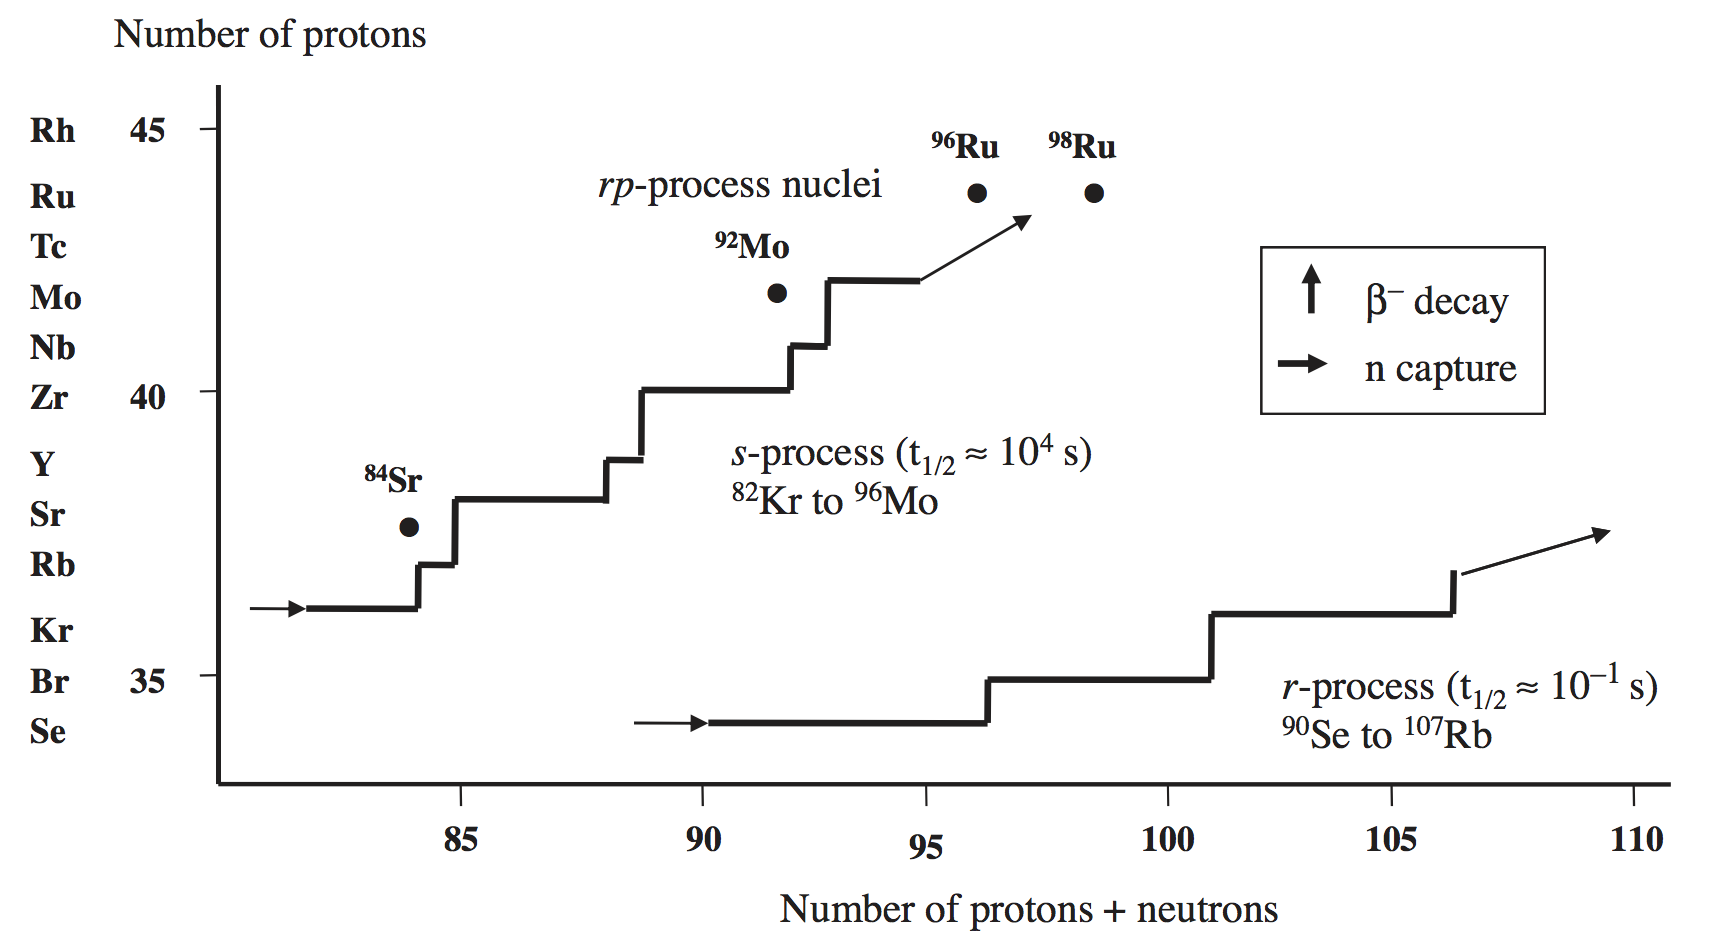
\includegraphics[width=14cm]{figures/rs-processes.png}
    \caption{\footnotesize{Sections of the tracks for the formation of heavy (trans-iron) elements along the r-process (rapid neutron capture, lower trace) and the s-process (slow neutron capture, upper trace). In both tracks, neutron capture is followed by $\beta^-$ decay (vertical lines); $t_{1/2}=$ half life. The dots represent nuclei that are formed by rapid proton capture (rp-process). Figure taken from Rehder (2010).}}
    \label{fig:rsprocesses}
\end{figure}

{\noindent}\textbf{Rapid processes}: The r-process, associated with very large neutron densities, requires a few seconds only. The timescale for neutron capture is $\sim10^{-4}\,{\rm s}$. Up to $10$ and more neutrons can be picked up before $\beta^-$ decay occurs when the neutron flux runs out. For neutron numbers per nucleus exceeding $184$, neutron-induced nuclear fission processes also come in, contributing to the distribution of the lighter r-process nuclei. Neutron capture at high temperature produces high-energy $\gamma$-rays; this leads to $(\gamma,n)$ photodisintegration competing with n-capture.

{\noindent}The explosive collapse of a pre-SN leaves behind a neutron core with an initial temperature of several $10^{11}\,{\rm K}$ that produces an extensive flux of neutrinos and anti-neutrinos with energies typically between $10$ and $20\,{\rm MeV}$. In proton-rich, cooler ejecta of the SNe, protons can be converted into neutrons by the absorption of anti-neutrinos. In principle, this is possible for free protons as well as for protons confined to nuclei. Since protons are sufficiently more abundant in the stellar envelopes than heavy nuclei, anti-neutrino capture occurs predominantly on free protons, leading to a drastic increase of neutron density for a few seconds, and subsequent neutron capture, in particular by nuclei that are comparatively proton-rich; that is, where the number of neutrons is about that of the number of protons. The net result of this process, termed $\nu$p-process, compares to that of the r- process. Along with the absorption of neutrons by neutron-deficient nuclei, neutron capture can also be coupled to the disposal of a proton. This $(n,p)$ reaction delivers nuclei with a higher effective cross section for proton capture, producing nuclei such as $^{92}$Mo, $^{94}$Mo, $^{96}$Ru, $^{98}$Ru, and $^{102}$Pd, which are otherwise not easily accessible.

{\noindent}\textbf{Slow processes}: In contrast to the rapid processes and typical of SNe scenarios, a slow neutron capture process is a characteristic event for the formation of trans-iron elements in the AGB phase of a star. In this phase (see track 4 in the HR diagram of Figure \ref{fig:hrd}), an extremely dense core primarily composed of carbon and oxygen is surrounded by a helium burning shell as the main source of energy and, slightly farther out, by a hydrogen burning shell followed by a tenuous hydrogen-rich envelope. When most of the helium has been consumed, the giant passes through a brief period of flickering (thermal pulses by alternately switching on and off H and He fusion), whereby material from the inner regions is mixed into the outer layers (\textbf{dredge-up}), and vice versa, accompanied by mass loss through violent stellar winds. The mass loss gives rise to a circumstellar envelope extending over several light-years.

{\noindent}In the s-process for which the neutron capture time is slow relative to the $\beta^-$ decay rates of the daughter nucleus, lower neutron densities and temperatures ($\sim3\times10^8\,{\rm K}$) than in the r-process are required.

% --------------------------------------------------------------
%               Resources 
% --------------------------------------------------------------

\newpage
\subsection{Resources}

\begin{itemize}
    \item Stellar Populations; Greggio \& Renzini (2011)
    \item The Fundamentals of Stellar Astrophysics, Collins (2003)
    \item Stellar Structure and Evolution, Kippenhahn, Weigert \& Weiss (2012)
    \item Evolution of Stars and Stellar Populations, Salaris \& Cassisi (2005)
    \item The Astronomical Reach of Fundamental Physics, Burrows \& Ostriker (2014)
    \item Opacity, Huebner \& Barfield (2014)
    \item Radiative Processes in Astrophysics, Rybicky \& Lightman (1979)
    \item Understanding Variable Stars, Percy (2007)
    \item A Library of Stellar Spectra; Jacoby \& Hunter (1984)
    \item A Digital Spectral Classification Atlas; Gray (2009)
    \item Notes on Star Formation; Krumholz (2015)
    \item Physics of the Interstellar and Intergalactic Medium; Draine (2011)
    \item Spectral Energy Distributions of T Tauri Stars with Passive Circumstellar Disks; Chiang \& Goldreich (1997)
    \item Fermi’s Paradox -- The Last Challenge for Copernicanism?; \'Cirkovi\'c (2009)
    \item Chemistry in Space: From Interstellar Matter to the Origin of Life; Rehder (2010)
    \item On the Anomalous Radii of the Transiting Extrasolar Planets; Laughlin et al. (2011)
    \item Possible Solutions to the Radius Anomalies of Transiting Giant Planets; Burrows et al. (2007)
    \item Re-Inflated Warm Jupiters Around Red Giants
\end{itemize}

\end{document}
